%&preformat-disser
\RequirePackage[l2tabu,orthodox]{nag} % Раскомментировав, можно в логе получать рекомендации относительно правильного использования пакетов и предупреждения об устаревших и нерекомендуемых пакетах
% Формат А4, 14pt (ГОСТ Р 7.0.11-2011, 5.3.6)
\documentclass[a4paper,14pt,oneside,openany]{memoir}

%%%%%%%%%%%%%%%%%%%%%%%%%%%%%%%%%%%%%%%%%%%%%%%%%%%%%%
%%%% Файл упрощённых настроек шаблона диссертации %%%%
%%%%%%%%%%%%%%%%%%%%%%%%%%%%%%%%%%%%%%%%%%%%%%%%%%%%%%

%%% Инициализирование переменных, не трогать!  %%%
\newcounter{intvl}
\newcounter{otstup}
\newcounter{contnumeq}
\newcounter{contnumfig}
\newcounter{contnumtab}
\newcounter{pgnum}
\newcounter{chapstyle}
\newcounter{headingdelim}
\newcounter{headingalign}
\newcounter{headingsize}
%%%%%%%%%%%%%%%%%%%%%%%%%%%%%%%%%%%%%%%%%%%%%%%%%%%%%%

%%% Область упрощённого управления оформлением %%%

%% Интервал между заголовками и между заголовком и текстом %%
% Заголовки отделяют от текста сверху и снизу
% тремя интервалами (ГОСТ Р 7.0.11-2011, 5.3.5)
\setcounter{intvl}{3}               % Коэффициент кратности к размеру шрифта

%% Отступы у заголовков в тексте %%
\setcounter{otstup}{0}              % 0 --- без отступа; 1 --- абзацный отступ

%% Нумерация формул, таблиц и рисунков %%
% Нумерация формул
\setcounter{contnumeq}{0}   % 0 --- пораздельно (во введении подряд,
                            %       без номера раздела);
                            % 1 --- сквозная нумерация по всей диссертации
% Нумерация рисунков
\setcounter{contnumfig}{0}  % 0 --- пораздельно (во введении подряд,
                            %       без номера раздела);
                            % 1 --- сквозная нумерация по всей диссертации
% Нумерация таблиц
\setcounter{contnumtab}{0}  % 0 --- пораздельно (во введении подряд,
                            %       без номера раздела);
                            % 1 --- сквозная нумерация по всей диссертации

%% Оглавление %%
\setcounter{pgnum}{1}       % 0 --- номера страниц никак не обозначены;
                            % 1 --- Стр. над номерами страниц (дважды
                            %       компилировать после изменения настройки)
\settocdepth{subsection}    % до какого уровня подразделов выносить в оглавление
\setsecnumdepth{subsection} % до какого уровня нумеровать подразделы


%% Текст и форматирование заголовков %%
\setcounter{chapstyle}{1}     % 0 --- разделы только под номером;
                              % 1 --- разделы с названием "Глава" перед номером
\setcounter{headingdelim}{1}  % 0 --- номер отделен пропуском в 1em или \quad;
                              % 1 --- номера разделов и приложений отделены
                              %       точкой с пробелом, подразделы пропуском
                              %       без точки;
                              % 2 --- номера разделов, подразделов и приложений
                              %       отделены точкой с пробелом.

%% Выравнивание заголовков в тексте %%
\setcounter{headingalign}{0}  % 0 --- по центру;
                              % 1 --- по левому краю

%% Размеры заголовков в тексте %%
\setcounter{headingsize}{0}   % 0 --- по ГОСТ, все всегда 14 пт;
                              % 1 --- пропорционально изменяющийся размер
                              %       в зависимости от базового шрифта

%% Подпись таблиц %%

% Смещение строк подписи после первой строки
\newcommand{\tabindent}{0cm}

% Тип форматирования заголовка таблицы:
% plain --- название и текст в одной строке
% split --- название и текст в разных строках
\newcommand{\tabformat}{plain}

%%% Настройки форматирования таблицы `plain`

% Выравнивание по центру подписи, состоящей из одной строки:
% true  --- выравнивать
% false --- не выравнивать
\newcommand{\tabsinglecenter}{false}

% Выравнивание подписи таблиц:
% justified   --- выравнивать как обычный текст («по ширине»)
% centering   --- выравнивать по центру
% centerlast  --- выравнивать по центру только последнюю строку
% centerfirst --- выравнивать по центру только первую строку (не рекомендуется)
% raggedleft  --- выравнивать по правому краю
% raggedright --- выравнивать по левому краю
\newcommand{\tabjust}{justified}

% Разделитель записи «Таблица #» и названия таблицы
\newcommand{\tablabelsep}{~\cyrdash\ }

%%% Настройки форматирования таблицы `split`

% Положение названия таблицы:
% \centering   --- выравнивать по центру
% \raggedleft  --- выравнивать по правому краю
% \raggedright --- выравнивать по левому краю
\newcommand{\splitformatlabel}{\raggedleft}

% Положение текста подписи:
% \centering   --- выравнивать по центру
% \raggedleft  --- выравнивать по правому краю
% \raggedright --- выравнивать по левому краю
\newcommand{\splitformattext}{\raggedright}

%% Подпись рисунков %%
%Разделитель записи «Рисунок #» и названия рисунка
\newcommand{\figlabelsep}{~\cyrdash\ }  % (ГОСТ 2.105, 4.3.1)
                                        % "--- здесь не работает

%%% Цвета гиперссылок %%%
% Latex color definitions: http://latexcolor.com/
\definecolor{linkcolor}{rgb}{0.9,0,0}
\definecolor{citecolor}{rgb}{0,0.6,0}
\definecolor{urlcolor}{rgb}{0,0,1}
%\definecolor{linkcolor}{rgb}{0,0,0} %black
%\definecolor{citecolor}{rgb}{0,0,0} %black
%\definecolor{urlcolor}{rgb}{0,0,0} %black
            % общие настройки шаблона
%%% Проверка используемого TeX-движка %%%
\newif\ifxetexorluatex   % определяем новый условный оператор (http://tex.stackexchange.com/a/47579)
\ifxetex
    \xetexorluatextrue
\else
    \ifluatex
        \xetexorluatextrue
    \else
        \xetexorluatexfalse
    \fi
\fi

\newif\ifsynopsis           % Условие, проверяющее, что документ~--- автореферат

\usepackage{etoolbox}[2015/08/02]   % Для продвинутой проверки разных условий
\providebool{presentation}

\usepackage{comment}    % Позволяет убирать блоки текста (добавляет
                        % окружение comment и команду \excludecomment)

%%% Поля и разметка страницы %%%
\usepackage{pdflscape}  % Для включения альбомных страниц
\usepackage{geometry}   % Для последующего задания полей

%%% Математические пакеты %%%
\usepackage{amsthm,amsmath,amscd}   % Математические дополнения от AMS
\usepackage{amsfonts,amssymb}       % Математические дополнения от AMS
\usepackage{mathtools}              % Добавляет окружение multlined
\usepackage{xfrac}                  % Красивые дроби
\usepackage[
    locale = DE,
    list-separator       = {;\,},
    list-final-separator = {;\,},
    list-pair-separator  = {;\,},
    list-units           = single,
    range-units          = single,
    range-phrase={\text{\ensuremath{-}}},
    % quotient-mode        = fraction, % красивые дроби могут не соответствовать ГОСТ
    fraction-function    = \sfrac,
    separate-uncertainty,
    ]{siunitx}[=v2]                 % Размерности SI
\sisetup{inter-unit-product = \ensuremath{{}\cdot{}}}

% Кириллица в нумерации subequations
% Для правильной работы требуется выполнение сразу после загрузки пакетов
\patchcmd{\subequations}{\def\theequation{\theparentequation\alph{equation}}}
{\def\theequation{\theparentequation\asbuk{equation}}}
{\typeout{subequations patched}}{\typeout{subequations not patched}}

%%%% Установки для размера шрифта 14 pt %%%%
%% Формирование переменных и констант для сравнения (один раз для всех подключаемых файлов)%%
%% должно располагаться до вызова пакета fontspec или polyglossia, потому что они сбивают его работу
\newlength{\curtextsize}
\newlength{\bigtextsize}
\setlength{\bigtextsize}{13.9pt}

\makeatletter
%\show\f@size    % неплохо для отслеживания, но вызывает стопорение процесса,
                 % если документ компилируется без команды  -interaction=nonstopmode
\setlength{\curtextsize}{\f@size pt}
\makeatother

%%% Кодировки и шрифты %%%
\ifxetexorluatex
    \ifpresentation
        \providecommand*\autodot{} % quick fix for polyglossia 1.50
    \fi
    \PassOptionsToPackage{no-math}{fontspec}    % https://tex.stackexchange.com/a/26295/104425
    \usepackage{polyglossia}[2014/05/21]        % Поддержка многоязычности
                                        % (fontspec подгружается автоматически)
\else
   %%% Решение проблемы копирования текста в буфер кракозябрами
    \ifnumequal{\value{usealtfont}}{0}{}{
        \input glyphtounicode.tex
        \input glyphtounicode-cmr.tex %from pdfx package
        \pdfgentounicode=1
    }
    \usepackage{cmap}   % Улучшенный поиск русских слов в полученном pdf-файле
    \ifnumequal{\value{usealtfont}}{2}{}{
        \defaulthyphenchar=127  % Если стоит до fontenc, то переносы
                                % не впишутся в выделяемый текст при
                                % копировании его в буфер обмена
    }
    \usepackage{textcomp}
    \usepackage[T1,T2A]{fontenc}                    % Поддержка русских букв
    \ifnumequal{\value{usealtfont}}{1}{% Используется pscyr, при наличии
        \IfFileExists{pscyr.sty}{\usepackage{pscyr}}{}  % Подключение pscyr
    }{}
    \usepackage[utf8]{inputenc}[2014/04/30]         % Кодировка utf8
    \usepackage[russian,main=english]{babel}[2014/03/24]% Языки: русский, английский
    \makeatletter\AtBeginDocument{\let\@elt\relax}\makeatother % babel 3.40 fix
    \ifnumequal{\value{usealtfont}}{2}{
        % http://dxdy.ru/post1238763.html#p1238763
        \usepackage[scaled=0.914]{XCharter}[2017/12/19] % Подключение русифицированных шрифтов XCharter
        \usepackage[charter, vvarbb, scaled=1.048]{newtxmath}[2017/12/14]
        \ifpresentation
        \else
            \setDisplayskipStretch{-0.078}
        \fi
    }{}
\fi

%%% Оформление абзацев %%%
\ifpresentation
\else
    \indentafterchapter     % Красная строка после заголовков типа chapter
    \usepackage{indentfirst}
\fi

%%% Цвета %%%
\ifpresentation
\else
    \usepackage[dvipsnames, table, hyperref]{xcolor} % Совместимо с tikz
\fi

%%% Таблицы %%%
\usepackage{longtable,ltcaption} % Длинные таблицы
\usepackage{multirow,makecell}   % Улучшенное форматирование таблиц
\usepackage{tabu, tabulary}      % таблицы с автоматически подбирающейся
                                 % шириной столбцов (tabu обязательно
                                 % до hyperref вызывать)
\makeatletter
%https://github.com/tabu-issues-for-future-maintainer/tabu/issues/26
\@ifpackagelater{longtable}{2020/02/07}{
\def\tabuendlongtrial{%
    \LT@echunk  \global\setbox\LT@gbox \hbox{\unhbox\LT@gbox}\kern\wd\LT@gbox
                \LT@get@widths
}%
}{}
\makeatother

\usepackage{threeparttable}      % автоматический подгон ширины подписи таблицы

%%% Общее форматирование
\usepackage{soulutf8}% Поддержка переносоустойчивых подчёркиваний и зачёркиваний
\usepackage{icomma}  % Запятая в десятичных дробях

%%% Оптимизация расстановки переносов и длины последней строки абзаца
\IfFileExists{impnattypo.sty}{% проверка установленности пакета impnattypo
    \ifluatex
        \ifnumequal{\value{draft}}{1}{% Черновик
            \usepackage[hyphenation, lastparline, nosingleletter, homeoarchy,
            rivers, draft]{impnattypo}
        }{% Чистовик
            \usepackage[hyphenation, lastparline, nosingleletter]{impnattypo}
        }
    \else
        \usepackage[hyphenation, lastparline]{impnattypo}
    \fi
}{}

%% Векторная графика

\usepackage{tikz}                   % Продвинутый пакет векторной графики
\usetikzlibrary{automata, positioning, arrows, shapes, calc, tikzmark, decorations.pathreplacing}

%%% Гиперссылки %%%
\ifxetexorluatex
    \let\CYRDZE\relax
\fi
\usepackage{hyperref}[2012/11/06]
% \renewcommand{\autoref}[1]{\fixme{autoref of }\ref{#1}}
\renewcommand{\autoref}[1]{\ref{#1}}

%%% Изображения %%%
\usepackage{graphicx}[2014/04/25]   % Подключаем пакет работы с графикой
\usepackage{caption}                % Подписи рисунков и таблиц
\usepackage{subcaption}             % Подписи подрисунков и подтаблиц
\usepackage{pdfpages}               % Добавление внешних pdf файлов

%%% Счётчики %%%
\usepackage{aliascnt}
\usepackage[figure,table]{totalcount}   % Счётчик рисунков и таблиц
\usepackage{totcount}   % Пакет создания счётчиков на основе последнего номера
                        % подсчитываемого элемента (может требовать дважды
                        % компилировать документ)
\usepackage{totpages}   % Счётчик страниц, совместимый с hyperref (ссылается
                        % на номер последней страницы). Желательно ставить
                        % последним пакетом в преамбуле

%%% Продвинутое управление групповыми ссылками (пока только формулами) %%%
\ifpresentation
\else
    \usepackage[english]{cleveref} % cleveref имеет сложности со считыванием
    % языка из babel. Такое решение русификации вывода выбрано вместо
    % определения в documentclass из опасности что-то лишнее передать во все
    % остальные пакеты, включая библиографию.

    % Добавление возможности использования пробелов в \labelcref
    % https://tex.stackexchange.com/a/340502/104425
    \usepackage{kvsetkeys}
    \makeatletter
    \let\org@@cref\@cref
    \renewcommand*{\@cref}[2]{%
        \edef\process@me{%
            \noexpand\org@@cref{#1}{\zap@space#2 \@empty}%
        }\process@me
    }
    \makeatother
\fi

\usepackage{placeins} % для \FloatBarrier

\ifnumequal{\value{draft}}{1}{% Черновик
    \usepackage[firstpage]{draftwatermark}
    \SetWatermarkText{DRAFT}
    \SetWatermarkFontSize{14pt}
    \SetWatermarkScale{15}
    \SetWatermarkAngle{45}
}{}

%%% Цитата, не приводимая в автореферате:
% возможно, актуальна только для biblatex
%\newcommand{\citeinsynopsis}[1]{\ifsynopsis\else ~\cite{#1} \fi}

% если текущий процесс запущен библиотекой tikz-external, то прекомпиляция должна быть включена
\ifdefined\tikzexternalrealjob
    \setcounter{imgprecompile}{1}
\fi

\ifnumequal{\value{imgprecompile}}{1}{% Только если у нас включена предкомпиляция
    \usetikzlibrary{external}   % подключение возможности предкомпиляции
    \tikzexternalize[prefix=images/cache/,optimize command away=\includepdf] % activate! % здесь можно указать отдельную папку для скомпилированных файлов
    \ifxetex
        \tikzset{external/up to date check={diff}}
    \fi
}{}
         % Пакеты общие для диссертации и автореферата
\synopsisfalse                      % Этот документ --- не автореферат
%%% Прикладные пакеты %%%
%\usepackage{calc}               % Пакет для расчётов параметров, например длины

%%% Для добавления Стр. над номерами страниц в оглавлении
%%% http://tex.stackexchange.com/a/306950
\usepackage{afterpage}

%%% Списки %%%
\usepackage{enumitem}

%%% Оформление списка обозначений
\usepackage[intoc]{nomencl}
\makenomenclature
\setlength{\nomitemsep}{-.8\parsep}
    % Пакеты для диссертации
\usepackage{fr-longtable}    %ради \endlasthead

% Листинги с исходным кодом программ
\usepackage{fancyvrb}
\usepackage{listings}
\lccode`\~=0\relax %Без этого хака из-за особенностей пакета listings перестают работать конструкции с \MakeLowercase и т. п. в (xe|lua)latex

% Русская традиция начертания греческих букв
\usepackage{upgreek} % прямые греческие ради русской традиции

%%% Микротипографика
%\ifnumequal{\value{draft}}{0}{% Только если у нас режим чистовика
%    \usepackage[final, babel, shrink=45]{microtype}[2016/05/14] % улучшает представление букв и слов в строках, может помочь при наличии отдельно висящих слов
%}{}

% Отметка о версии черновика на каждой странице
% Чтобы работало надо в своей локальной копии по инструкции
% https://www.ctan.org/pkg/gitinfo2 создать небходимые файлы в папке
% ./git/hooks
% If you’re familiar with tweaking git, you can probably work it out for
% yourself. If not, I suggest you follow these steps:
% 1. First, you need a git repository and working tree. For this example,
% let’s suppose that the root of the working tree is in ~/compsci
% 2. Copy the file post-xxx-sample.txt (which is in the same folder of
% your TEX distribution as this pdf) into the git hooks directory in your
% working copy. In our example case, you should end up with a file called
% ~/compsci/.git/hooks/post-checkout
% 3. If you’re using a unix-like system, don’t forget to make the file executable.
% Just how you do this is outside the scope of this manual, but one
% possible way is with commands such as this:
% chmod g+x post-checkout.
% 4. Test your setup with “git checkout master” (or another suitable branch
% name). This should generate copies of gitHeadInfo.gin in the directories
% you intended.
% 5. Now make two more copies of this file in the same directory (hooks),
% calling them post-commit and post-merge, and you’re done. As before,
% users of unix-like systems should ensure these files are marked as
% executable.
\ifnumequal{\value{draft}}{1}{% Черновик
   \IfFileExists{.git/gitHeadInfo.gin}{
      \usepackage[mark,pcount]{gitinfo2}
      \renewcommand{\gitMark}{rev.\gitAbbrevHash\quad\gitCommitterEmail\quad\gitAuthorIsoDate}
      \renewcommand{\gitMarkFormat}{\rmfamily\color{Gray}\small\bfseries}
   }{}
}{}

\usepackage{stmaryrd}
\usepackage{thm-restate}
\usepackage{pgfplots}
\usepackage{minted}
\usepackage{multicol}
\usepackage{diagbox}

\newcolumntype{x}[1]{>{\centering\let\newline\\\arraybackslash\hspace{0pt}}p{#1}}

\usepackage[vlined,linesnumbered]{algorithm2e}
\DontPrintSemicolon{}
\SetNlSty{bfseries}{\color{black}}{}
\SetKwIF{If}{ElseIf}{Else}{if}{the}{elif}{else}{}
\SetKwFor{For}{for}{}{}
\SetKwFor{While}{while}{}{}
\SetKwInput{KwData}{Параметры}
\SetKw{Halt}{halt}
% \SetAlgoSkip{}
\SetKwInput{KwIn}{Input}
\SetKwInput{KwOut}{Output}
\SetKwInput{KwData}{Parameters}
\SetKw{Return}{return}
\renewcommand{\algorithmcfname}{Algorithm}
\renewcommand*{\proofname}{Proof}

% makes optional title of theorems bold by default
\makeatletter
\def\th@plain{%
  \thm@notefont{}% same as heading font
  \itshape % body font
}
\def\th@definition{%
  \thm@notefont{}% same as heading font
  \normalfont % body font
}
\makeatother
\theoremstyle{definition}
\newtheorem{theorem}{Theorem}
\newtheorem{lemma}{Lemma}
\newtheorem{corollary}{Corollary}
\newtheorem{proposition}{Proposition}
\newtheorem{rmk}{Remark}
\newtheorem{problem}{Problem}
\newtheorem{restrict}{Restriction}
\newtheorem{axiom}{Axiom}
\newtheorem{example}{Example}
\newtheorem{define}{Definition}
\newtheorem{rewriting}{Rewriting rule}
\newtheorem{resquest}{Research question}

\usepackage{float}
\floatstyle{boxed}
\newfloat{mylisting}{tbph}{lol}[chapter]
\floatname{mylisting}{Listing}

\makeatletter
\renewcommand*{\float@listhead}[1]{%
  \@ifundefined{chapter}{%
    \section*{#1}%
    \addcontentsline{toc}{section}{#1}%
  }{%
    \chapter*{#1}%
    \addcontentsline{toc}{chapter}{#1}%
  }%
  \@mkboth{\MakeUppercase{#1}}{\MakeUppercase{#1}}%
}
\makeatother   % Пакеты для специфических пользовательских задач

%%%%%%%%%%%%%%%%%%%%%%%%%%%%%%%%%%%%%%%%%%%%%%%%%%%%%%
%%%% Файл упрощённых настроек шаблона диссертации %%%%
%%%%%%%%%%%%%%%%%%%%%%%%%%%%%%%%%%%%%%%%%%%%%%%%%%%%%%

%%% Инициализирование переменных, не трогать!  %%%
\newcounter{intvl}
\newcounter{otstup}
\newcounter{contnumeq}
\newcounter{contnumfig}
\newcounter{contnumtab}
\newcounter{pgnum}
\newcounter{chapstyle}
\newcounter{headingdelim}
\newcounter{headingalign}
\newcounter{headingsize}
%%%%%%%%%%%%%%%%%%%%%%%%%%%%%%%%%%%%%%%%%%%%%%%%%%%%%%

%%% Область упрощённого управления оформлением %%%

%% Интервал между заголовками и между заголовком и текстом %%
% Заголовки отделяют от текста сверху и снизу
% тремя интервалами (ГОСТ Р 7.0.11-2011, 5.3.5)
\setcounter{intvl}{3}               % Коэффициент кратности к размеру шрифта

%% Отступы у заголовков в тексте %%
\setcounter{otstup}{0}              % 0 --- без отступа; 1 --- абзацный отступ

%% Нумерация формул, таблиц и рисунков %%
% Нумерация формул
\setcounter{contnumeq}{0}   % 0 --- пораздельно (во введении подряд,
                            %       без номера раздела);
                            % 1 --- сквозная нумерация по всей диссертации
% Нумерация рисунков
\setcounter{contnumfig}{0}  % 0 --- пораздельно (во введении подряд,
                            %       без номера раздела);
                            % 1 --- сквозная нумерация по всей диссертации
% Нумерация таблиц
\setcounter{contnumtab}{0}  % 0 --- пораздельно (во введении подряд,
                            %       без номера раздела);
                            % 1 --- сквозная нумерация по всей диссертации

%% Оглавление %%
\setcounter{pgnum}{1}       % 0 --- номера страниц никак не обозначены;
                            % 1 --- Стр. над номерами страниц (дважды
                            %       компилировать после изменения настройки)
\settocdepth{subsection}    % до какого уровня подразделов выносить в оглавление
\setsecnumdepth{subsection} % до какого уровня нумеровать подразделы


%% Текст и форматирование заголовков %%
\setcounter{chapstyle}{1}     % 0 --- разделы только под номером;
                              % 1 --- разделы с названием "Глава" перед номером
\setcounter{headingdelim}{1}  % 0 --- номер отделен пропуском в 1em или \quad;
                              % 1 --- номера разделов и приложений отделены
                              %       точкой с пробелом, подразделы пропуском
                              %       без точки;
                              % 2 --- номера разделов, подразделов и приложений
                              %       отделены точкой с пробелом.

%% Выравнивание заголовков в тексте %%
\setcounter{headingalign}{0}  % 0 --- по центру;
                              % 1 --- по левому краю

%% Размеры заголовков в тексте %%
\setcounter{headingsize}{0}   % 0 --- по ГОСТ, все всегда 14 пт;
                              % 1 --- пропорционально изменяющийся размер
                              %       в зависимости от базового шрифта

%% Подпись таблиц %%

% Смещение строк подписи после первой строки
\newcommand{\tabindent}{0cm}

% Тип форматирования заголовка таблицы:
% plain --- название и текст в одной строке
% split --- название и текст в разных строках
\newcommand{\tabformat}{plain}

%%% Настройки форматирования таблицы `plain`

% Выравнивание по центру подписи, состоящей из одной строки:
% true  --- выравнивать
% false --- не выравнивать
\newcommand{\tabsinglecenter}{false}

% Выравнивание подписи таблиц:
% justified   --- выравнивать как обычный текст («по ширине»)
% centering   --- выравнивать по центру
% centerlast  --- выравнивать по центру только последнюю строку
% centerfirst --- выравнивать по центру только первую строку (не рекомендуется)
% raggedleft  --- выравнивать по правому краю
% raggedright --- выравнивать по левому краю
\newcommand{\tabjust}{justified}

% Разделитель записи «Таблица #» и названия таблицы
\newcommand{\tablabelsep}{~\cyrdash\ }

%%% Настройки форматирования таблицы `split`

% Положение названия таблицы:
% \centering   --- выравнивать по центру
% \raggedleft  --- выравнивать по правому краю
% \raggedright --- выравнивать по левому краю
\newcommand{\splitformatlabel}{\raggedleft}

% Положение текста подписи:
% \centering   --- выравнивать по центру
% \raggedleft  --- выравнивать по правому краю
% \raggedright --- выравнивать по левому краю
\newcommand{\splitformattext}{\raggedright}

%% Подпись рисунков %%
%Разделитель записи «Рисунок #» и названия рисунка
\newcommand{\figlabelsep}{~\cyrdash\ }  % (ГОСТ 2.105, 4.3.1)
                                        % "--- здесь не работает

%%% Цвета гиперссылок %%%
% Latex color definitions: http://latexcolor.com/
\definecolor{linkcolor}{rgb}{0.9,0,0}
\definecolor{citecolor}{rgb}{0,0.6,0}
\definecolor{urlcolor}{rgb}{0,0,1}
%\definecolor{linkcolor}{rgb}{0,0,0} %black
%\definecolor{citecolor}{rgb}{0,0,0} %black
%\definecolor{urlcolor}{rgb}{0,0,0} %black
      % Упрощённые настройки шаблона

% Новые переменные, которые могут использоваться во всём проекте
% ГОСТ 7.0.11-2011
% 9.2 Оформление текста автореферата диссертации
% 9.2.1 Общая характеристика работы включает в себя следующие основные структурные
% элементы:
% актуальность темы исследования;
\newcommand{\actualityTXT}{Актуальность темы.}
% степень ее разработанности;
\newcommand{\progressTXT}{Степень разработанности темы.}
% цели и задачи;
\newcommand{\aimTXT}{Целью}
\newcommand{\tasksTXT}{задачи}
% научную новизну;
\newcommand{\noveltyTXT}{Научная новизна}
% теоретическую и практическую значимость работы;
\newcommand{\influenceTXT}{Теоретическая и практическая значимость работы.}
\newcommand{\influencePrTXT}{Практическая значимость работы.}
\newcommand{\influenceThTXT}{Теоретическая значимость работы.}
% или чаще используют просто
% \newcommand{\influenceTXT}{Практическая значимость}
% методологию и методы исследования;
\newcommand{\methodsTXT}{Методология и методы исследования.}
% положения, выносимые на защиту;
\newcommand{\defpositionsTXT}{Основные положения, выносимые на~защиту.}
% степень достоверности и апробацию результатов.
\newcommand{\reliabilityTXT}{Достоверность}
\newcommand{\probationTXT}{Апробация работы.}

\newcommand{\contributionTXT}{Личный вклад}
\newcommand{\publicationsTXT}{Публикации.}


%%% Заголовки библиографии:

% для автореферата:
\newcommand{\bibtitleauthor}{Публикации автора по теме диссертации}

% для стиля библиографии `\insertbiblioauthorgrouped`
\newcommand{\bibtitleauthorvak}{В изданиях из списка ВАК РФ}
\newcommand{\bibtitleauthorscopus}{В изданиях, входящих в международную базу цитирования Scopus}
\newcommand{\bibtitleauthorwos}{В изданиях, входящих в международную базу цитирования Web of Science}
\newcommand{\bibtitleauthorother}{В прочих изданиях}
\newcommand{\bibtitleauthorconf}{В сборниках трудов конференций}
\newcommand{\bibtitleauthorpatent}{Зарегистрированные патенты}
\newcommand{\bibtitleauthorprogram}{Зарегистрированные программы для ЭВМ}

% для стиля библиографии `\insertbiblioauthorimportant`:
\newcommand{\bibtitleauthorimportant}{Наиболее значимые \protect\MakeLowercase\bibtitleauthor}

% для списка литературы в диссертации и списка чужих работ в автореферате:
\newcommand{\bibtitlefull}{Список литературы} % (ГОСТ Р 7.0.11-2011, 4)


\newcommand{\pdr}{IC3/PDR}
\newcommand{\cegar}{CEGAR}
\newcommand{\ice}{ICE}
\newcommand{\fmf}{FMF}
\newcommand{\satur}{Насыщение}

\newcommand{\zprover}{\textsc{Z3}}
\newcommand{\cvc}{\textsc{cvc5}}
\newcommand{\princess}{\textsc{Princess}}
\newcommand{\chaff}{\textsc{Chaff}}
\newcommand{\cvcind}{\textsc{\cvc{}-Ind}}
\newcommand{\mace}{\textsc{Mace4}}
\newcommand{\kodkod}{\textsc{Kodkod}}
\newcommand{\paradox}{\textsc{Paradox}}
\newcommand{\vampire}{\textsc{Vampire}}
\newcommand{\eprover}{\textsc{E}}
\newcommand{\zipperposition}{\textsc{Zipperposition}}

\newcommand{\eldarica}{\textsc{Eldarica}}
\newcommand{\theringen}{\textsc{RInGen}}
\newcommand{\ringenAny}[2]{#1(#2)}
\newcommand{\ringenSyncAny}[1]{\textsc{#1-Sync}}
\newcommand{\theringenCICIAny}[1]{\textsc{#1-CICI}}
\newcommand{\ringenCICIAny}[2]{\theringenCICIAny{#1}(#2)}
\newcommand{\ringen}[1]{\ringenAny{\theringen}{#1}}
\newcommand{\ringenSync}{\ringenSyncAny{\theringen}}
\newcommand{\theringenCICI}{\theringenCICIAny{\theringen}}
\newcommand{\ringenCICI}[1]{\ringenCICIAny{\theringen}{#1}}
\newcommand{\verifier}{\mathcal{V}}
\newcommand{\spacer}{\textsc{Spacer}}
\newcommand{\racer}{\textsc{Racer}}
\newcommand{\hoice}{\textsc{HoIce}}
\newcommand{\rchc}{\textsc{RCHC}}
\newcommand{\vericat}{\textsc{VeriCaT}}
\newcommand{\verimap}{\textsc{VeriMAP-iddt}}

\newcommand{\chccomp}{CHC-COMP}

\newcommand{\haskell}{\textsc{Haskell}}
\newcommand{\ocaml}{\textsc{OCaml}}
\newcommand{\fstar}{\textsc{F*}}
\newcommand{\fsharp}{\textsc{F\#}}
\newcommand{\clanguage}{\textsc{C}}
\newcommand{\cplusplus}{\textsc{C++}}
\newcommand{\rust}{\textsc{Rust}}
\newcommand{\scala}{\textsc{Scala}}

\newcommand{\liquidHaskell}{\textsc{LiquidHaskell}}
\newcommand{\flux}{\textsc{Flux}}
\newcommand{\leon}{\textsc{Leon}}
\newcommand{\stainless}{\textsc{Stainless}}
\newcommand{\rcaml}{\textsc{RCaml}}
\newcommand{\dafny}{\textsc{Dafny}}
\newcommand{\whyThree}{\textsc{Why3}}
\newcommand{\viper}{\textsc{Viper}}
\newcommand{\coq}{\textsc{Coq}}
\newcommand{\idris}{\textsc{Idris}}
\newcommand{\agda}{\textsc{Agda}}
\newcommand{\lean}{\textsc{Lean}}
\newcommand{\solidity}{\textsc{Solidity}}
\newcommand{\rustHorn}{\textsc{RustHorn}}
\newcommand{\solCMC}{\textsc{SolCMC}}

\newcommand{\theregclass}{Reg}
\newcommand{\regclass}{\textsc{\theregclass{}}}
\newcommand{\theelemclass}{Elem}
\newcommand{\elemclass}{\textsc{\theelemclass{}}}
\newcommand{\elemextclass}{\textsc{\theelemclass{}\textsubscript{*}}}
\newcommand{\sizeelemclass}{\textsc{Size\theelemclass{}}}
\newcommand{\sizeelemextclass}{\textsc{Size\theelemclass{}\textsubscript{*}}}
\newcommand{\catelemclass}{\textsc{Cat\theelemclass{}}}
\newcommand{\syncRegFlatClass}{\regclass{}\textsubscript{+}} %TODO: take it from Haudebourg
\newcommand{\syncRegFullClass}{\regclass{}\textsubscript{$\times$}}
\newcommand{\regelemclass}{\textsc{\theelemclass{}\theregclass{}}}

\newcommand{\signature}{\Sigma}

\newcommand{\structure}{\mathcal{M}}
\newcommand{\relations}{\mathcal{R}}
\newcommand{\prog}{\mathcal{P}}
\newcommand{\states}{\mathcal{S}}
\newcommand{\functions}{\mathcal{F}}
\newcommand{\hs}{\mathcal{H}}
\newcommand{\diseqsem}[1]{\mathcal{D}_{\sigma_{#1}}}
\newcommand{\diseqsemh}[1]{\widehat{\mathcal{D}}_{\sigma_{#1}}}
\newcommand{\height}[1]{\mathcal{H}eight(#1)}
\newcommand{\invClass}{\mathcal{I}}
\newcommand{\theterms}{\mathcal{T}}
\newcommand{\thelang}{\mathcal{L}}
\newcommand{\langOf}[1]{\thelang\left(#1\right)}
\newcommand{\classOf}[1]{\regclass_{#1}}

\newcommand{\formallang}{\mathbf{L}}

\newcommand{\termsOfSize}[2]{\mathbb{T}_{#1}^{#2}}
\newcommand{\sizesOfSort}[1]{\mathbb{S}_{#1}}

% CHC examples
\newcommand{\exRef}[1]{\hyperref[ex:#1]{\textit{#1}}}
\newcommand{\exEvenLeft}{\exRef{even}}
\newcommand{\exLR}{\exRef{lr}}
\newcommand{\exLt}{\exRef{lt}}
\newcommand{\exNode}{\exRef{node}}

% DT defs
\newcommand{\natDef}{$Nat ::= Z \mid S\ Nat$}

% Transition systems
\newcommand{\csubseteq}{\subseteq}
\newcommand{\cbot}{0}
\newcommand{\ctop}{1}
\newcommand{\ccap}{\cap}
\newcommand{\ccup}{\cup}
\newcommand{\cneg}{\neg}
\newcommand{\csetminus}{\setminus}
\newcommand{\init}{Init}
\newcommand{\thepost}{T}
\newcommand{\theapost}{\hat{T}}
\newcommand{\post}[1]{\thepost\left(#1\right)}
\newcommand{\apost}[1]{\theapost\left(#1\right)}
\newcommand{\property}{Prop}
\newcommand{\theAbstrDomain}{A}
\newcommand{\abstrDomain}{\mathcal{\theAbstrDomain}}
\newcommand{\asubseteq}{\sqsubseteq}
\newcommand{\abot}{\bot_{\abstrDomain}}
\renewcommand{\atop}{\top_{\abstrDomain}}
\newcommand{\acap}{\sqcap}
\newcommand{\acup}{\sqcup}

% CEGAR(O)
\newcommand{\oracle}{\mathcal{O}}
\newcommand{\theRunBlackBox}{Collaborate}
\newcommand{\RunBlackBox}{\textsc{\theRunBlackBox}}
\newcommand{\substituteLemmas}{\textsc{ResidualCHCs}}
\newcommand{\simplifiedSubstituteLemmas}[1]{Q\left(#1\right)}
\newcommand{\ourCEGAR}{\cegar{}($\oracle$)}
\newcommand{\theBlackBoxDomain}{B}
\newcommand{\blackBoxDomain}{\mathcal{\theBlackBoxDomain}}
\newcommand{\evenInv}{\mathcal{E}}

\newcommand{\fsymbs}{\signature_F}
\newcommand{\psymbs}{\signature_P}
\newcommand{\sorts}{\signature_S}
\newcommand{\groundTerms}{\theterms(\fsymbs)}
\newcommand{\groundTermsStar}{\theterms(\fsymbs^{\leq k})}
% \newcommand{\autBot}{\perp\!\!\!\perp}
% \newcommand{\autBotOp}[1]{\operatorname{\autBot}\big(#1\big)}
% \newcommand{\autBotInv}[1]{\operatorname{\autBot^{-1}}\big(#1\big)}
% \newcommand{\fsymbsBot}{\fsymbs^{\autBot}}
% \newcommand{\groundTermsBot}{\theterms(\fsymbsBot)}
% \newcommand{\groundTermsPower}[1]{\theterms^{#1}(\fsymbsBot)}
% \newcommand{\groundTermsMatrix}[2]{\groundTermsPower{#1\times #2}}
% \newcommand{\groundTermsNM}{\groundTermsMatrix{n}{m}}
\newcommand{\btuple}[1]{\big\langle #1 \big\rangle}
\newcommand{\tuple}[1]{\left\langle #1 \right\rangle}
\newcommand{\sizeofSet}[1]{\left|#1\right|}
\newcommand{\thedomain}{\sizeofSet{\structure}}
\newcommand{\domainOf}[2]{\sizeofSet{#1}_{#2}}
\newcommand{\domain}[1]{\domainOf{\structure}{#1}}
\newcommand{\huniv}[1]{\domainOf{\hs}{#1}}
\newcommand{\interprets}[2]{#1\llbracket #2\rrbracket}
\newcommand{\clforall}[1]{\forall{#1}}
\newcommand{\theautomaton}[4]{\btuple{#1, #2, #3, #4}}
\newcommand{\autInit}{s_0}
\newcommand{\autStates}{S}
\newcommand{\autFinStates}{\autStates_F}
\newcommand{\autTrans}{\Delta}
\newcommand{\autApp}[1]{A\left(#1\right)}
\newcommand{\automaton}[3]{\theautomaton{#1}{\fsymbs}{#2}{#3}}
\newcommand{\automatonDef}{\automaton{\autStates}{\autFinStates}{\autTrans}}
\newcommand{\Automaton}[2]{\automaton{\{#1\}}{\{#2\}}{\autTrans}}
\newcommand{\sautomatonGen}[4]{\theautomaton{#1}{\fsymbs^{\leq #2}}{#3}{#4}}
\newcommand{\sautomaton}[3]{\sautomatonGen{\{#1\}}{#2}{\{#3\}}{\autTrans}}
% \newcommand{\sautomatonDef}{\sautomaton{\autStates}{\autFinStates}{\autInit{}}}
% \newcommand{\SautomatonGen}[4]{\sautomatonGen{\{#1\}}{\{#2\}}{#3}{#4}}
% \newcommand{\Sautomaton}[3]{\SautomatonGen{#1}{#2}{#3}{\autTrans}}
\newcommand{\eqdef}{\triangleq}
\newcommand{\eqby}[1]{\mathrel{\stackrel{\mbox{\normalfont\tiny #1}}{=}}}
\newcommand{\body}[1]{body\left(#1\right)}
\newcommand{\rules}[1]{rules\left(#1\right)}
\newcommand{\conv}{\sigma}
\newcommand{\fullConv}{\conv_{fc}}
\newcommand{\flatConv}{\conv_{sc}}
\newcommand{\oneConv}{\conv_{lc}}
\newcommand{\quotient}[2]{{#1}/{#2}}

\newcommand{\subterm}[2]{#2\left(#1\right)}
\newcommand{\leafpos}[2]{\mathit{leaves}_{#1}(#2)}
\newcommand{\sizename}[0]{size}
\newcommand{\maxFinSize}[1]{\operatorname{max}_{fin}\big(#1\big)}

\newcommand{\booleanOp}{\bowtie}         % Новые переменные, для всего проекта
\newcommand{\exampleTwo} % Even
{
\begin{center}
\begin{tikzpicture}[shorten >=1pt,node distance=2cm,on grid,auto,scale=0.8,every node/.style={scale=0.8}]
    \node[state,initial,accepting,initial text=$Z$] (s0) {$s_0$};
    \node[state] (s1) [right=of s0] {$s_1$};
    \path[->]
        (s0)    edge [bend left=25] node {$S$}       (s1)
        (s1)    edge [bend left=25] node {$S$}       (s0)
    ;
\end{tikzpicture}
\end{center}
}
\newcommand{\forkJoinExample} % Even
{%
\begin{center}%
\begin{tikzpicture}[shorten >=1pt,node distance=4cm,on grid,auto,scale=1.0,every node/.style={scale=1.0}]
    \node[state,initial,accepting,initial text=$Seq$] (s0) {$s_0$};
    \node[state] (s1) [right=of s0] {$s_1$};
    \path[->]
        (s0)    edge [bend left=25] node {$Join$}       (s1)
        (s1)    edge [bend left=25] node {$Fork$}       (s0)
    ;
\end{tikzpicture}%
\end{center}%
}

\newcommand{\exampleOne}{\begin{center} % inc % 3
  \begin{tikzpicture}[shorten >=1pt,node distance=2cm,on grid,auto,scale=0.8,every node/.style={scale=0.8}]
      \node[state,initial,initial text=Z] (s0) {$s_0$};
      \node[state] (s1) [above right=0.25cm and 2cm of s0] {$s_1$};
      \node[state] (s2) [below right=0.25cm and 2cm of s1] {$s_2$};
      % \node[state,accepting] (s3) [right=of s2] {$s_3$};
      % \node[state] (s4) [right=of s3] {$s_4$};
      \path[->]
          (s0)    edge  [bend left=25]  node {$S$}      (s1)
          (s1)    edge   [bend left=25]            node {$S$}      (s2)
          (s2)    edge   [bend left=15]            node {$S$}         (s0)
          % (s0) edge [below] node {$*$} (s4)
      ;
  \end{tikzpicture}
  \end{center}%
  }

  \newcommand{\newworkflowWithTestersAndSelectors}
{%
\begin{figure}[h]
\centering
\tikzset{every picture/.style={line width=0.75pt}} %set default line width to 0.75pt        

\begin{tikzpicture}[x=0.75pt,y=0.75pt,yscale=-1.3,xscale=1.3, every node/.style={scale=0.7}]
%uncomment if require: \path (0,300); %set diagram left start at 0, and has height of 300

%Rounded Rect [id:dp6178352482663523] 
\draw   (43.5,62.63) .. controls (43.5,57.86) and (47.36,54) .. (52.13,54) -- (167.88,54) .. controls (172.64,54) and (176.5,57.86) .. (176.5,62.63) -- (176.5,88.5) .. controls (176.5,93.26) and (172.64,97.13) .. (167.88,97.13) -- (52.13,97.13) .. controls (47.36,97.13) and (43.5,93.26) .. (43.5,88.5) -- cycle ;
%Rounded Rect [id:dp31517424205318467] 
\draw   (229,61.83) .. controls (229,56.95) and (232.95,53) .. (237.83,53) -- (349.68,53) .. controls (354.55,53) and (358.5,56.95) .. (358.5,61.83) -- (358.5,88.3) .. controls (358.5,93.17) and (354.55,97.13) .. (349.68,97.13) -- (237.83,97.13) .. controls (232.95,97.13) and (229,93.17) .. (229,88.3) -- cycle ;
%Rounded Rect [id:dp03467191946149972] 
\draw   (409,60.3) .. controls (409,55.23) and (413.11,51.13) .. (418.18,51.13) -- (524.33,51.13) .. controls (529.39,51.13) and (533.5,55.23) .. (533.5,60.3) -- (533.5,87.83) .. controls (533.5,92.89) and (529.39,97) .. (524.33,97) -- (418.18,97) .. controls (413.11,97) and (409,92.89) .. (409,87.83) -- cycle ;
%Rounded Rect [id:dp5801423669885661] 
\draw   (124,144.9) .. controls (124,140.05) and (127.93,136.13) .. (132.78,136.13) -- (222.73,136.13) .. controls (227.57,136.13) and (231.5,140.05) .. (231.5,144.9) -- (231.5,171.23) .. controls (231.5,176.07) and (227.57,180) .. (222.73,180) -- (132.78,180) .. controls (127.93,180) and (124,176.07) .. (124,171.23) -- cycle ;
%Rounded Rect [id:dp6969866775126601] 
\draw   (301,145.03) .. controls (301,140.04) and (305.04,136) .. (310.02,136) -- (448.48,136) .. controls (453.46,136) and (457.5,140.04) .. (457.5,145.03) -- (457.5,172.1) .. controls (457.5,177.08) and (453.46,181.13) .. (448.48,181.13) -- (310.02,181.13) .. controls (305.04,181.13) and (301,177.08) .. (301,172.1) -- cycle ;

\draw (471.25,74.06) node   [align=left] {First-order formula\\over free theory}; %без $\displaystyle \neq $,\\тестеров и селекторов};
% Text Node
\draw (110,75.56) node   [align=left] {Horn clauses over ADT};
% Text Node
\draw (295.75,75.06) node   [align=left] {Horn clauses over \\ ADT without constraints}; %$\displaystyle \neq $,\\тестеров и селекторов};
% Text Node
\draw (177.75,157) node   [align=left] {Final model};
% Text Node
\draw (379.25,158.56) node   [align=left] {Tree automaton\\($\displaystyle \Rightarrow $ Regular invariant)};

% % Text Node
% \draw (471.25,74.06) node   [align=left,execute at begin node=\setlength{\baselineskip}{1ex}] {CHCs over EUF\\without $\displaystyle \neq $, testers\\and selectors};
% % Text Node
% \draw (110,75.56) node   [align=left] {CHCs over ADTs};
% % Text Node
% \draw (295.75,75.06) node   [align=left,execute at begin node=\setlength{\baselineskip}{1ex}] {CHCs over ADTs\\without $\displaystyle \neq $, testers\\and selectors};
% % Text Node
% \draw (177.75,157) node   [align=left] {Finite model};
% % Text Node
% \draw (379.25,158.56) node   [align=left] {Tree tuples automata\\($\displaystyle \Rightarrow $Herbrand model)};
% Connection
\draw    (174.5,75.38) -- node[above] {Sec.~\ref{sec:fmf/totalCorrectness}} (233.25,75.25);
\draw [shift={(235.25,75.25)}, rotate = 539.8299999999999] [color={rgb, 255:red, 0; green, 0; blue, 0 }  ][line width=0.75]    (10.93,-3.29) .. controls (6.95,-1.4) and (3.31,-0.3) .. (0,0) .. controls (3.31,0.3) and (6.95,1.4) .. (10.93,3.29)   ;
% Connection
\draw    (356.25,74.72) -- node[above] {Sec.~\ref{sec:fmf/partialCorrectness}} (411.25,74.4) ;
\draw [shift={(413.25,74.39)}, rotate = 539.6700000000001] [color={rgb, 255:red, 0; green, 0; blue, 0 }  ][line width=0.75]    (10.93,-3.29) .. controls (6.95,-1.4) and (3.31,-0.3) .. (0,0) .. controls (3.31,0.3) and (6.95,1.4) .. (10.93,3.29)   ;
% Connection
\draw    (413.25,91.58) .. controls (295.23,130.94) and (243.1,115.96) .. node[above,rotate=10] {Finite model finding} (201.55,143.65) ;
\draw [shift={(200.29,144.5)}, rotate = 325.36] [color={rgb, 255:red, 0; green, 0; blue, 0 }  ][line width=0.75]    (10.93,-3.29) .. controls (6.95,-1.4) and (3.31,-0.3) .. (0,0) .. controls (3.31,0.3) and (6.95,1.4) .. (10.93,3.29)   ;
% Connection
\draw    (230,157.35) -- node[above] {Th.~\ref{thm:finite-to-automaton}} (300.75,157.95) ;
\draw [shift={(302.75,157.97)}, rotate = 180.44] [color={rgb, 255:red, 0; green, 0; blue, 0 }  ][line width=0.75]    (10.93,-3.29) .. controls (6.95,-1.4) and (3.31,-0.3) .. (0,0) .. controls (3.31,0.3) and (6.95,1.4) .. (10.93,3.29)   ;
\end{tikzpicture}
\caption{Regular invariant inference method for a Horn clause system over ADT}
\label{fig:newworkflow-with-testers-selectors}
\end{figure}%
}

\newcommand{\exampleCostruction}
{
\begin{center}
\begin{tikzpicture}[shorten >=1pt,node distance=2cm,on grid,auto,scale=0.8,every node/.style={scale=0.8}]
    \node[state,initial,accepting,initial text=$Z$] (s0) {$0$};
    \node[state] (s1) [right=of s0] {$1$};
    \path[->]
        (s0)    edge [bend left=25] node {$S$}       (s1)
        (s1)    edge [bend left=25] node {$S$}       (s0)
    ;
\end{tikzpicture}
\end{center}
}

\newcommand{\defPumpLemmaElem}{%
\begin{restatable}[Pumping Lemma for \elemclass{}]{lemma}{pumplemmaelem}\label{lemm:pump-elem}
Let $\formallang{}$ be an elementary language of $n$-tuples. Then,
\begin{itemize}
    \item there exists a constant $K > 0$ satisfying:
    \item for every $n$-tuples of ground terms $\tuple{g_1,\ldots,g_n} \in \formallang{}$,
    \item for any $i$ such that $\height{g_i} > K$,
    \item for all infinite sorts $\sigma \in \sorts$ and
    \item for all paths $p$ with a length greater than $K$,
    \item there exist finite sets of paths $P_j$ such that $p \in P_i$,
    \item for all $p_1, p_2 \in \bigcup_j P_j$ it is true that $p_1(g) = p_2(g)$,
    \item and there is $N \geq 0$, such that
    \item for all $t$ of sort $\sigma$ with $\height{t} > N$ it holds that:
\end{itemize}
$$\tuple{g_1[P_1\leftarrow t],\ldots,g_i[P_i\leftarrow t],\ldots,g_n[P_n\leftarrow t]} \in \formallang{}.$$
\end{restatable}
}

\newcommand{\defPumpLemmaSizeElem}{%
\begin{restatable}[Pumping Lemma for \sizeelemclass{}]{lemma}{pumplemmasizeelem}\label{lemm:pump-sizeelem}
Let the ADT signature be expanding and let $\formallang{}$ be an elementary language of $n$-tuples with size constraints. Then,
\begin{itemize}
\item there exists a constant $K > 0$ satisfying:
\item for every $n$-tuple of ground terms $\tuple{g_1,\ldots,g_n} \in \formallang{}$,
\item for any $i$, such that $\height{g_i} > K$,
\item for all infinite sorts $\sigma \in \sorts$, and
\item for all paths $p \in \leafpos{\sigma}{g_i}$ with length greater than $K$,
\item there exists an infinite linear set $T \subseteq \sizesOfSort{\sigma}$, such that
\item for all terms $t$ of sort $\sigma$ with sizes $\sizename{}(t) \in T$,
\item there exist sequences of paths $P_j$, with no path in them being a suffix of path $p$,
\item and sequences of terms $U_j$, such that
\end{itemize}
$$\tuple{g_1[P_1\!\leftarrow\! U_1],\ldots,g_i[p \!\leftarrow\! t, P_i \!\leftarrow\! U_i],\ldots,g_n[P_n \!\leftarrow\! U_n]} \in \formallang{}.$$
\end{restatable}
}

\newcommand{\invariantreprclasses}[1]
{
\begin{figure}[t]
\tikzset{every picture/.style={line width=0.75pt}} %set default line width to 0.75pt       
\centering
\begin{tikzpicture}[shorten >=1pt,auto,node distance=15mm,scale=1.0,every state/.style={scale=1.0,minimum width=26mm}]
    \node[state] (regElem) {\regelemclass{}};
    \node (regElemL) [left=of regElem] {};
    \node (regElemR) [right=of regElem] {};
    \node[state] (elem) [below=of regElemL] {\elemclass{}};
    \node[state] (reg) [below=of regElemR] {\regclass{}};
    \node[state] (sizeelem) [left=of regElemL] {\sizeelemclass{}};
    \node[state] (syncFlat) [right=of regElemR] {\syncRegFlatClass{}};
    \node[state] (syncFull) [above=of syncFlat] {\syncRegFullClass{}};
    \path[->]
        (elem)    edge node {\exLt}       (sizeelem)
        (elem)    edge node {\exEvenLeft\footnotemark}       (regElem)
        (reg)    edge node {\exLR\footnotemark}       (regElem)
        (reg)    edge node {\exLt\footnotemark}       (syncFlat)
        (syncFlat)    edge node {\exNode\footnotemark}       (syncFull)
    ;
\end{tikzpicture}
\caption{Inclusion relations between classes of inductive invariants over ADTs.}%Связи включения между классами индуктивных инвариантов над АТД. 
#1
\end{figure}
\footnotetext[1]{$\exEvenLeft{} \in \regclass{} \setminus \sizeelemclass{}$ (Theorem~\ref{thm:exEvenLeft})}
\footnotetext[2]{$\exLR{}\in\elemclass{} \setminus \syncRegFullClass{}$ (Lemma~\ref{lemm:lr-not-in-reg-full})}
\footnotetext[3]{$\exLt\in\syncRegFlatClass{}\setminus\regclass{}$ (Theorem~\ref{thm:exLt})}
\footnotetext[4]{$\exNode\in\syncRegFullClass{}\setminus\syncRegFlatClass{}$ (Lemma~\ref{lemm:node-not-in-reg-flat})}
}

\newcommand{\toolplotOne}{
\pgfplotstableread[col sep = comma]{Dissertation/images/experiments1.csv}\all
\begin{figure}[t!]
\begin{center}
\begin{tikzpicture}[scale=1.2]
\begin{axis}[xmode=log, ymode=log, legend pos= north west, xlabel={Runtime of \ringen{\cvc{}}, ms}, xlabel style = {align=center,font=\footnotesize}, ylabel style = {align=center,font=\footnotesize}, ylabel={Runtime of {\color{red}\racer{}}, {\color{blue}\eldarica{}},\\{\color{brown}\cvcind{}} and {\color{cyan}\verimap{}}, ms}]
% \begin{axis}[xmode=log, ymode=log, legend pos= north west, xlabel={ Regular model construction by \theringen{}}, ylabel style = {align=center}, ylabel={Elementary model construction by \\{\color{red}\textsc{Spacer}}, {\color{blue}\eldarica{}} and {\color{brown}\cvcind{}}}]
    \addplot[dashed,no marks,very thin] coordinates {(10,10) (600000,600000)};
    \addplot [dashed, no marks, thin] coordinates {(10,10) (600000,600000)};
    \addplot [dashed, no marks, thin] coordinates {(10,300000) (300000,300000)};
    \addplot [dashed, no marks, thin] coordinates {(300000, 10) (300000,300000)};
    \addplot [dashed, no marks, thin] coordinates {(10, 600000) (600000,600000)};
    \addplot [dashed, no marks, thin] coordinates {(600000, 10) (600000,600000)};

    \addplot  [only marks,  mark=triangle, color=blue, mark size=3pt] table [x={CVC4Finite}, y={Eldarica}] {\all};
    \addplot  [only marks,  mark=o, color=red,  mark size=3pt] table [x={CVC4Finite}, y={Z3}] {\all};
    \addplot  [only marks,  mark=x, color=brown, mark size=3pt] table [x={CVC4Finite}, y={CVC4Ind}] {\all};
    \addplot  [only marks,  mark=square, color=cyan, mark size=3pt] table [x={CVC4Finite}, y={VeriMAP-iddt}] {\all};
\end{axis}

\end{tikzpicture}
    \caption{ Performance comparison. Each point on the plot represents a pair of runtimes.} %Сравнение производительности инструментов. Каждая точка на графике представляет пару длительностей выполнения.
\label{fig:toolplotOne}
\end{center}
\end{figure}
}

\newcommand{\fmfModelSizes}{
\pgfplotstableread[col sep = comma]{Dissertation/images/cards.csv}\all
\begin{figure}[ht!]
\begin{center}

\begin{tikzpicture}[scale=1.0]
  \begin{axis}[
  xlabel={Размер модели},
  ylabel={Число моделей},
  ybar,
  xtick distance=1,
  ytick distance=1,
    ]
    \addplot+ table {\all};
  \end{axis}
\end{tikzpicture}
\caption{Размеры конечных моделей, построенных инструментом \cvc{}~--- сторонним решателем, вызываемым инструментом \theringen{}. Размер модели (на оси абсцисс) считается как \emph{сумма} мощностей всех сортов.}
\label{fig:cardinalities}
\end{center}
\end{figure}
}

\newcommand{\toolplotsatOne}{
\pgfplotstableread[col sep = comma]{Dissertation/images/expsat1.csv}\allsat
\begin{figure}[t!]
\begin{center}
\begin{tikzpicture}[scale=1.2]
\begin{axis}[xmode=log, ymode=log, legend pos= north west, xlabel={Время построения регулярных инвариантов\\при помощи \theringen{}, сек.}, xlabel style = {align=center,font=\footnotesize}, ylabel style = {align=center,font=\footnotesize}, ylabel={Время построения элементарных\\инвариантов при помощи {\color{red}\zprover{}}, {\color{blue}\eldarica{}},\\{\color{brown}\cvcind{}} и {\color{cyan}\verimap{}}, сек.}]
    \addplot[dashed,no marks,very thin] coordinates {(10,10) (600000,600000)};
    \addplot [dashed, no marks, thin] coordinates {(10,10) (600000,600000)};
    \addplot [dashed, no marks, thin] coordinates {(10,300000) (300000,300000)};
    \addplot [dashed, no marks, thin] coordinates {(300000, 10) (300000,300000)};
    \addplot [dashed, no marks, thin] coordinates {(10, 600000) (600000,600000)};
    \addplot [dashed, no marks, thin] coordinates {(600000, 10) (600000,600000)};

    \addplot  [only marks,  mark=triangle, color=blue, mark size=3pt] table [x={CVC4Finite}, y={Eldarica}] {\allsat};
    \addplot  [only marks,  mark=o, color=red,  mark size=3pt] table [x={CVC4Finite}, y={Z3}] {\allsat};
    \addplot  [only marks,  mark=x, color=brown, mark size=3pt] table [x={CVC4Finite}, y={CVC4Ind}] {\allsat};
    \addplot  [only marks,  mark=square, color=cyan, mark size=3pt] table [x={CVC4Finite}, y={VeriMAP-iddt}] {\allsat};
\end{axis}
\end{tikzpicture}
    \caption{Сравнение производительности инструментов \emph{только на результатах \foreignlanguage{english}{<<SAT>>}}. Тест включается в этот график, если хотя бы один из инструментов обнаружил инвариант.}
\label{fig:toolplotsat}
\end{center}
\end{figure}
}

\newcommand{\toolplotTwo}[2]{%
% #1 is backend solver name
% #2 is a .csv file name
\pgfplotstableread[col sep = comma]{#2}\toolplotcsv
\begin{subfigure}[t]{0.49\textwidth}
\begin{center}
\begin{tikzpicture}[scale=.95]
\begin{axis}[xmode=log, ymode=log, legend pos= north west, xlabel={\ringenCICI{#1}, ms}, ylabel style = {align=center}, ylabel={{\color{red}\racer{}} and {\color{blue}\ringen{#1}}, ms}]
    \addplot[dashed,no marks,very thin] coordinates {(10,10) (1200000,1200000)};
    \addplot [dashed, no marks, thin] coordinates {(10,10) (1200000,1200000)};
    \addplot [dashed, no marks, thin] coordinates {(10,600000) (600000,600000)};
    \addplot [dashed, no marks, thin] coordinates {(600000, 10) (600000,600000)};
    \addplot [dashed, no marks, thin] coordinates {(10, 1200000) (1200000,1200000)};
    \addplot [dashed, no marks, thin] coordinates {(1200000, 10) (1200000,1200000)};
    
    % one second
    \addplot [no marks, thin] coordinates {(1000, 10) (1000,1000)};
    \addplot [no marks, thin] coordinates {(10, 1000) (1000,1000)};

    \addplot  [only marks,  mark=o, color=red,  mark size=3pt] table [x={Collab}, y={Z3}] {\toolplotcsv};
    \addplot  [only marks,  mark=triangle, color=blue, mark size=3pt] table [x={Collab}, y={RInGen}] {\toolplotcsv};
\end{axis}
\end{tikzpicture}
\end{center}
\end{subfigure}
}

\newcommand{\PattternAutomata}{
    \begin{figure*}[h]
    \centering
    \begin{tikzpicture}[node distance=2cm,remember picture]
    
    \node (A) at (1,0) {$Node$};
    \node (B) at (0,-1){$x$};
    \node (B1) at (-0.5,-2){$x_1$};
    \node (B2) at (0.5,-2){$x_2$};
    
    \node (C) at (2,-1){$y$};
    \node (C1) at (1.5,-2){$y_1$};
    \node (C2) at (2.5,-2){$y_2$};
    
    \draw[-] (A) -- (B);
    \draw[-] (A) -- (C);
    \draw[-] (B) -- (B1);
    \draw[-] (B) -- (B2);
    
    \draw[-] (C) -- (C1);
    \draw[-] (C) -- (C2);
    
    \node (D) at (6,0) {$z$};
    \node (E) at (5,-1){$g$};
    \node (F) at (7,-1){$h$};
    \node (E1) at (4.5,-2){$g_1$};
    \node (E2) at (5.5,-2){$g_2$};
    
    \node (F1) at (6.5,-2){$h_1$};
    \node (F2) at (7.5,-2){$h_2$};
    
    \draw[-] (D) -- (E);
    \draw[-] (D) -- (F);
    \draw[-] (E) -- (E1);
    \draw[-] (E) -- (E2);
    \draw[-] (F) -- (F1);
    \draw[-] (F) -- (F2);
    
    \end{tikzpicture}
    \label{fig:ref-stdSync}
    \end{figure*}
    }

\newcommand{\ltAutomaton}{
    \begin{figure}[h]
    \centering
    \begin{tikzpicture}[scale=1]
 
    \node [state] {$q_0$};
    \node (q0) [state,
    initial,
    initial left,
    initial distance=0.5cm,
    initial text=$\tuple{\bot, \bot}$
] {$q_0$};
    \node (q1) [state, accepting] at (3,1) {$q_1$};
    \node (q2) [state] at (3,-1) {$q_2$};

    \path [-stealth, thick]
        (q0) edge [bend left] node [above] {$\tuple{\bot, Z}$}   (q1)
        (q0) edge [bend right] node [below] {$\tuple{Z, \bot}$}   (q2)
        (q1) edge [loop right]  node {*}()
        (q2) edge [loop right]  node {*}();

    \end{tikzpicture}
    %\caption{Синхронный древовидный автомат для предикатного символа $lt$}\label{fig:ltAutomata}
    \end{figure}
}         % Новые переменные, для всего проекта

%%% Основные сведения %%%
\newcommand{\thesisAuthorLastName}{Костюков}
\newcommand{\thesisAuthorOtherNames}{Юрий Олегович}
\newcommand{\thesisAuthorInitials}{Ю.\,О.}
\newcommand{\thesisAuthor}             % Диссертация, ФИО автора
{%
    \texorpdfstring{% \texorpdfstring takes two arguments and uses the first for (La)TeX and the second for pdf
        \thesisAuthorLastName~\thesisAuthorOtherNames% так будет отображаться на титульном листе или в тексте, где будет использоваться переменная
    }{%
        \thesisAuthorLastName, \thesisAuthorOtherNames% эта запись для свойств pdf-файла. В таком виде, если pdf будет обработан программами для сбора библиографических сведений, будет правильно представлена фамилия.
    }
}
\newcommand{\thesisAuthorShort}        % Диссертация, ФИО автора инициалами
{\thesisAuthorInitials~\thesisAuthorLastName}
%\newcommand{\thesisUdk}                % Диссертация, УДК
%{\fixme{xxx.xxx}}
\newcommand{\thesisTitle}              % Диссертация, название
{Автоматический вывод индуктивных инвариантов программ с~алгебраическими типами данных}
\newcommand{\thesisSpecialtyNumber}    % Диссертация, специальность, номер
{\fixme{XX.XX.XX}}
\newcommand{\thesisSpecialtyTitle}     % Диссертация, специальность, название (название взято с сайта ВАК для примера)
{\fixme{Информатика}}
%% \newcommand{\thesisSpecialtyTwoNumber} % Диссертация, вторая специальность, номер
%% {\fixme{XX.XX.XX}}
%% \newcommand{\thesisSpecialtyTwoTitle}  % Диссертация, вторая специальность, название
%% {\fixme{Теория и~методика физического воспитания, спортивной тренировки,
%% оздоровительной и~адаптивной физической культуры}}
\newcommand{\thesisDegree}             % Диссертация, ученая степень
{кандидата физико-математических наук}
\newcommand{\thesisDegreeShort}        % Диссертация, ученая степень, краткая запись
{канд. физ.-мат. наук}
\newcommand{\thesisCity}               % Диссертация, город написания диссертации
{Санкт-Петербург}
\newcommand{\thesisYear}               % Диссертация, год написания диссертации
{2023}
\newcommand{\thesisOrganization}       % Диссертация, организация
{Федеральное государственное бюджетное образовательное учреждение высшего
образования <<Санкт-Петербургский государственный университет СПбГУ>>}
\newcommand{\thesisOrganizationShort}  % Диссертация, краткое название организации для доклада
{\fixme{НазУчДисРаб}}

\newcommand{\thesisInOrganization}     % Диссертация, организация в предложном падеже: Работа выполнена *макрос*.
{на кафедре системного программирования федерального государственного бюджетного образовательного учреждения высшего образования <<Санкт-Петербургский государственный университет>>}

%% \newcommand{\supervisorDead}{}           % Рисовать рамку вокруг фамилии
\newcommand{\supervisorFio}              % Научный руководитель, ФИО
{Кознов Дмитрий Владимирович}
\newcommand{\supervisorRegalia}          % Научный руководитель, регалии
{Доктор технических наук, Санкт-Петербургский государственный университет, профессор кафедры системного программирования}
\newcommand{\supervisorFioShort}         % Научный руководитель, ФИО
{Д.\,В.~Кознов}
\newcommand{\supervisorRegaliaShort}     % Научный руководитель, регалии
{\fixme{уч.~ст.,~уч.~зв.}}

%% \newcommand{\supervisorTwoDead}{}        % Рисовать рамку вокруг фамилии
\newcommand{\supervisorTwoFio}           % Второй научный руководитель, ФИО
{Мордвинов Дмитрий Александрович}
\newcommand{\supervisorTwoRegalia}       % Второй научный руководитель, регалии
{Канд. физ.-мат. наук, Санкт-Петербургский государственный университет, доцент кафедры системного программирования}
\newcommand{\supervisorTwoFioShort}      % Второй научный руководитель, ФИО
{Д.\,А.~Мордвинов}
\newcommand{\supervisorTwoRegaliaShort}  % Второй научный руководитель, регалии
{\fixme{уч.~ст.,~уч.~зв.}}

\newcommand{\opponentOneFio}           % Оппонент 1, ФИО
{\fixme{Фамилия Имя Отчество}}
\newcommand{\opponentOneRegalia}       % Оппонент 1, регалии
{\fixme{доктор физико-математических наук, профессор}}
\newcommand{\opponentOneJobPlace}      % Оппонент 1, место работы
{\fixme{Не очень длинное название для места работы}}
\newcommand{\opponentOneJobPost}       % Оппонент 1, должность
{\fixme{старший научный сотрудник}}

\newcommand{\opponentTwoFio}           % Оппонент 2, ФИО
{\fixme{Фамилия Имя Отчество}}
\newcommand{\opponentTwoRegalia}       % Оппонент 2, регалии
{\fixme{кандидат физико-математических наук}}
\newcommand{\opponentTwoJobPlace}      % Оппонент 2, место работы
{\fixme{Основное место работы c длинным длинным длинным длинным названием}}
\newcommand{\opponentTwoJobPost}       % Оппонент 2, должность
{\fixme{старший научный сотрудник}}

%% \newcommand{\opponentThreeFio}         % Оппонент 3, ФИО
%% {\fixme{Фамилия Имя Отчество}}
%% \newcommand{\opponentThreeRegalia}     % Оппонент 3, регалии
%% {\fixme{кандидат физико-математических наук}}
%% \newcommand{\opponentThreeJobPlace}    % Оппонент 3, место работы
%% {\fixme{Основное место работы c длинным длинным длинным длинным названием}}
%% \newcommand{\opponentThreeJobPost}     % Оппонент 3, должность
%% {\fixme{старший научный сотрудник}}

\newcommand{\leadingOrganizationTitle} % Ведущая организация, дополнительные строки. Удалить, чтобы не отображать в автореферате
{\fixme{Федеральное государственное бюджетное образовательное учреждение высшего
профессионального образования с~длинным длинным длинным длинным названием}}

\newcommand{\defenseDate}              % Защита, дата
{\fixme{DD mmmmmmmm YYYY~г.~в~XX часов}}
\newcommand{\defenseCouncilNumber}     % Защита, номер диссертационного совета
{\fixme{Д\,123.456.78}}
\newcommand{\defenseCouncilTitle}      % Защита, учреждение диссертационного совета
{\fixme{Название учреждения}}
\newcommand{\defenseCouncilAddress}    % Защита, адрес учреждение диссертационного совета
{\fixme{Адрес}}
\newcommand{\defenseCouncilPhone}      % Телефон для справок
{\fixme{+7~(0000)~00-00-00}}

\newcommand{\defenseSecretaryFio}      % Секретарь диссертационного совета, ФИО
{\fixme{Фамилия Имя Отчество}}
\newcommand{\defenseSecretaryRegalia}  % Секретарь диссертационного совета, регалии
{\fixme{д-р~физ.-мат. наук}}            % Для сокращений есть ГОСТы, например: ГОСТ Р 7.0.12-2011 + http://base.garant.ru/179724/#block_30000

\newcommand{\synopsisLibrary}          % Автореферат, название библиотеки
{\fixme{Название библиотеки}}
\newcommand{\synopsisDate}             % Автореферат, дата рассылки
{\fixme{DD mmmmmmmm}\the\year~года}

% To avoid conflict with beamer class use \providecommand
\providecommand{\keywords}%            % Ключевые слова для метаданных PDF диссертации и автореферата
{}
             % Основные сведения
%%% Кодировки и шрифты %%%
\ifxetexorluatex
    % Язык по-умолчанию русский с поддержкой приятных команд пакета babel
    \setmainlanguage{english}
    % Дополнительный язык = английский (в американской вариации по-умолчанию)
    \setotherlanguage[babelshorthands=true]{russian}

    % Проверка существования шрифтов. Недоступна в pdflatex
    \ifnumequal{\value{fontfamily}}{1}{
        \IfFontExistsTF{Times New Roman}{}{\setcounter{fontfamily}{0}}
    }{}
    \ifnumequal{\value{fontfamily}}{2}{
        \IfFontExistsTF{LiberationSerif}{}{\setcounter{fontfamily}{0}}
    }{}

    \ifnumequal{\value{fontfamily}}{0}{                    % Семейство шрифтов CMU. Используется как fallback
        \setmonofont{CMU Typewriter Text}                  % моноширинный шрифт
        \newfontfamily\cyrillicfonttt{CMU Typewriter Text} % моноширинный шрифт для кириллицы
        \defaultfontfeatures{Ligatures=TeX}                % стандартные лигатуры TeX, замены нескольких дефисов на тире и т. п. Настройки моноширинного шрифта должны идти до этой строки, чтобы при врезках кода программ в коде не применялись лигатуры и замены дефисов
        \setmainfont{CMU Serif}                            % Шрифт с засечками
        \newfontfamily\cyrillicfont{CMU Serif}             % Шрифт с засечками для кириллицы
        \setsansfont{CMU Sans Serif}                       % Шрифт без засечек
        \newfontfamily\cyrillicfontsf{CMU Sans Serif}      % Шрифт без засечек для кириллицы
    }

    \ifnumequal{\value{fontfamily}}{1}{                    % Семейство MS шрифтов
        \setmonofont{Courier New}                          % моноширинный шрифт
        \newfontfamily\cyrillicfonttt{Courier New}         % моноширинный шрифт для кириллицы
        \defaultfontfeatures{Ligatures=TeX}                % стандартные лигатуры TeX, замены нескольких дефисов на тире и т. п. Настройки моноширинного шрифта должны идти до этой строки, чтобы при врезках кода программ в коде не применялись лигатуры и замены дефисов
        \setmainfont{Times New Roman}                      % Шрифт с засечками
        \newfontfamily\cyrillicfont{Times New Roman}       % Шрифт с засечками для кириллицы
        \setsansfont{Arial}                                % Шрифт без засечек
        \newfontfamily\cyrillicfontsf{Arial}               % Шрифт без засечек для кириллицы
    }

    \ifnumequal{\value{fontfamily}}{2}{                    % Семейство шрифтов Liberation (https://pagure.io/liberation-fonts)
        \setmonofont{LiberationMono}[Scale=0.87] % моноширинный шрифт
        \newfontfamily\cyrillicfonttt{LiberationMono}[     % моноширинный шрифт для кириллицы
            Scale=0.87]
        \defaultfontfeatures{Ligatures=TeX}                % стандартные лигатуры TeX, замены нескольких дефисов на тире и т. п. Настройки моноширинного шрифта должны идти до этой строки, чтобы при врезках кода программ в коде не применялись лигатуры и замены дефисов
        \setmainfont{LiberationSerif}                      % Шрифт с засечками
        \newfontfamily\cyrillicfont{LiberationSerif}       % Шрифт с засечками для кириллицы
        \setsansfont{LiberationSans}                       % Шрифт без засечек
        \newfontfamily\cyrillicfontsf{LiberationSans}      % Шрифт без засечек для кириллицы
    }

\else
    \ifnumequal{\value{usealtfont}}{1}{% Используется pscyr, при наличии
        \IfFileExists{pscyr.sty}{\renewcommand{\rmdefault}{ftm}}{}
    }{}
\fi
            % Определение шрифтов (частичное)
%%% Шаблон %%%
\DeclareRobustCommand{\fixme}{\textcolor{red}}  % решаем проблему превращения
                                % названия цвета в результате \MakeUppercase,
                                % http://tex.stackexchange.com/a/187930,
                                % \DeclareRobustCommand protects \fixme
                                % from expanding inside \MakeUppercase
\AtBeginDocument{%
    \setlength{\parindent}{2.5em}                   % Абзацный отступ. Должен быть одинаковым по всему тексту и равен пяти знакам (ГОСТ Р 7.0.11-2011, 5.3.7).
}

%%% Таблицы %%%
\DeclareCaptionLabelSeparator{tabsep}{\tablabelsep} % нумерация таблиц
\DeclareCaptionFormat{split}{\splitformatlabel#1\par\splitformattext#3}

\captionsetup[table]{
        format=\tabformat,                % формат подписи (plain|hang)
        font=normal,                      % нормальные размер, цвет, стиль шрифта
        skip=.0pt,                        % отбивка под подписью
        parskip=.0pt,                     % отбивка между параграфами подписи
        position=above,                   % положение подписи
        justification=\tabjust,           % центровка
        indent=\tabindent,                % смещение строк после первой
        labelsep=tabsep,                  % разделитель
        singlelinecheck=\tabsinglecenter, % не выравнивать по центру, если умещается в одну строку
}

%%% Рисунки %%%
\DeclareCaptionLabelSeparator{figsep}{\figlabelsep} % нумерация рисунков

\captionsetup[figure]{
        format=plain,                     % формат подписи (plain|hang)
        font=normal,                      % нормальные размер, цвет, стиль шрифта
        skip=.0pt,                        % отбивка под подписью
        parskip=.0pt,                     % отбивка между параграфами подписи
        position=below,                   % положение подписи
        singlelinecheck=true,             % выравнивание по центру, если умещается в одну строку
        justification=centerlast,         % центровка
        labelsep=figsep,                  % разделитель
}

%%% Подписи подрисунков %%%
\DeclareCaptionSubType{figure}
\renewcommand\thesubfigure{\asbuk{subfigure}} % нумерация подрисунков
\ifsynopsis
\DeclareCaptionFont{norm}{\fontsize{10pt}{11pt}\selectfont}
\newcommand{\subfigureskip}{2.pt}
\else
\DeclareCaptionFont{norm}{\fontsize{14pt}{16pt}\selectfont}
\newcommand{\subfigureskip}{0.pt}
\fi

\captionsetup[subfloat]{
        labelfont=norm,                 % нормальный размер подписей подрисунков
        textfont=norm,                  % нормальный размер подписей подрисунков
        labelsep=space,                 % разделитель
        labelformat=brace,              % одна скобка справа от номера
        justification=centering,        % центровка
        singlelinecheck=true,           % выравнивание по центру, если умещается в одну строку
        skip=\subfigureskip,            % отбивка над подписью
        parskip=.0pt,                   % отбивка между параграфами подписи
        position=below,                 % положение подписи
}

%%% Настройки ссылок на рисунки, таблицы и др. %%%
% команды \cref...format отвечают за форматирование при помощи команды \cref
% команды \labelcref...format отвечают за форматирование при помощи команды \labelcref

\ifpresentation
\else
    \crefdefaultlabelformat{#2#1#3}

    % Уравнение
    \crefformat{equation}{(#2#1#3)} % одиночная ссылка с приставкой
    \labelcrefformat{equation}{(#2#1#3)} % одиночная ссылка без приставки
    \crefrangeformat{equation}{(#3#1#4) \textendash~(#5#2#6)} % диапазон ссылок с приставкой
    \labelcrefrangeformat{equation}{(#3#1#4) \textendash~(#5#2#6)} % диапазон ссылок без приставки
    \crefmultiformat{equation}{(#2#1#3)}{ и~(#2#1#3)}{, (#2#1#3)}{ и~(#2#1#3)} % перечисление ссылок с приставкой
    \labelcrefmultiformat{equation}{(#2#1#3)}{ и~(#2#1#3)}{, (#2#1#3)}{ и~(#2#1#3)} % перечисление без приставки

    % Подуравнение
    \crefformat{subequation}{(#2#1#3)} % одиночная ссылка с приставкой
    \labelcrefformat{subequation}{(#2#1#3)} % одиночная ссылка без приставки
    \crefrangeformat{subequation}{(#3#1#4) \textendash~(#5#2#6)} % диапазон ссылок с приставкой
    \labelcrefrangeformat{subequation}{(#3#1#4) \textendash~(#5#2#6)} % диапазон ссылок без приставки
    \crefmultiformat{subequation}{(#2#1#3)}{ и~(#2#1#3)}{, (#2#1#3)}{ и~(#2#1#3)} % перечисление ссылок с приставкой
    \labelcrefmultiformat{subequation}{(#2#1#3)}{ и~(#2#1#3)}{, (#2#1#3)}{ и~(#2#1#3)} % перечисление без приставки

    % Глава
    \crefformat{chapter}{#2#1#3} % одиночная ссылка с приставкой
    \labelcrefformat{chapter}{#2#1#3} % одиночная ссылка без приставки
    \crefrangeformat{chapter}{#3#1#4 \textendash~#5#2#6} % диапазон ссылок с приставкой
    \labelcrefrangeformat{chapter}{#3#1#4 \textendash~#5#2#6} % диапазон ссылок без приставки
    \crefmultiformat{chapter}{#2#1#3}{ и~#2#1#3}{, #2#1#3}{ и~#2#1#3} % перечисление ссылок с приставкой
    \labelcrefmultiformat{chapter}{#2#1#3}{ и~#2#1#3}{, #2#1#3}{ и~#2#1#3} % перечисление без приставки

    % Параграф
    \crefformat{section}{#2#1#3} % одиночная ссылка с приставкой
    \labelcrefformat{section}{#2#1#3} % одиночная ссылка без приставки
    \crefrangeformat{section}{#3#1#4 \textendash~#5#2#6} % диапазон ссылок с приставкой
    \labelcrefrangeformat{section}{#3#1#4 \textendash~#5#2#6} % диапазон ссылок без приставки
    \crefmultiformat{section}{#2#1#3}{ и~#2#1#3}{, #2#1#3}{ и~#2#1#3} % перечисление ссылок с приставкой
    \labelcrefmultiformat{section}{#2#1#3}{ и~#2#1#3}{, #2#1#3}{ и~#2#1#3} % перечисление без приставки

    % Приложение
    \crefformat{appendix}{#2#1#3} % одиночная ссылка с приставкой
    \labelcrefformat{appendix}{#2#1#3} % одиночная ссылка без приставки
    \crefrangeformat{appendix}{#3#1#4 \textendash~#5#2#6} % диапазон ссылок с приставкой
    \labelcrefrangeformat{appendix}{#3#1#4 \textendash~#5#2#6} % диапазон ссылок без приставки
    \crefmultiformat{appendix}{#2#1#3}{ и~#2#1#3}{, #2#1#3}{ и~#2#1#3} % перечисление ссылок с приставкой
    \labelcrefmultiformat{appendix}{#2#1#3}{ и~#2#1#3}{, #2#1#3}{ и~#2#1#3} % перечисление без приставки

    % Рисунок
    \crefformat{figure}{#2#1#3} % одиночная ссылка с приставкой
    \labelcrefformat{figure}{#2#1#3} % одиночная ссылка без приставки
    \crefrangeformat{figure}{#3#1#4 \textendash~#5#2#6} % диапазон ссылок с приставкой
    \labelcrefrangeformat{figure}{#3#1#4 \textendash~#5#2#6} % диапазон ссылок без приставки
    \crefmultiformat{figure}{#2#1#3}{ и~#2#1#3}{, #2#1#3}{ и~#2#1#3} % перечисление ссылок с приставкой
    \labelcrefmultiformat{figure}{#2#1#3}{ и~#2#1#3}{, #2#1#3}{ и~#2#1#3} % перечисление без приставки

    % Таблица
    \crefformat{table}{#2#1#3} % одиночная ссылка с приставкой
    \labelcrefformat{table}{#2#1#3} % одиночная ссылка без приставки
    \crefrangeformat{table}{#3#1#4 \textendash~#5#2#6} % диапазон ссылок с приставкой
    \labelcrefrangeformat{table}{#3#1#4 \textendash~#5#2#6} % диапазон ссылок без приставки
    \crefmultiformat{table}{#2#1#3}{ и~#2#1#3}{, #2#1#3}{ и~#2#1#3} % перечисление ссылок с приставкой
    \labelcrefmultiformat{table}{#2#1#3}{ и~#2#1#3}{, #2#1#3}{ и~#2#1#3} % перечисление без приставки

    % Листинг
    \crefformat{lstlisting}{#2#1#3} % одиночная ссылка с приставкой
    \labelcrefformat{lstlisting}{#2#1#3} % одиночная ссылка без приставки
    \crefrangeformat{lstlisting}{#3#1#4 \textendash~#5#2#6} % диапазон ссылок с приставкой
    \labelcrefrangeformat{lstlisting}{#3#1#4 \textendash~#5#2#6} % диапазон ссылок без приставки
    \crefmultiformat{lstlisting}{#2#1#3}{ и~#2#1#3}{, #2#1#3}{ и~#2#1#3} % перечисление ссылок с приставкой
    \labelcrefmultiformat{lstlisting}{#2#1#3}{ и~#2#1#3}{, #2#1#3}{ и~#2#1#3} % перечисление без приставки

    % Листинг
    \crefformat{ListingEnv}{#2#1#3} % одиночная ссылка с приставкой
    \labelcrefformat{ListingEnv}{#2#1#3} % одиночная ссылка без приставки
    \crefrangeformat{ListingEnv}{#3#1#4 \textendash~#5#2#6} % диапазон ссылок с приставкой
    \labelcrefrangeformat{ListingEnv}{#3#1#4 \textendash~#5#2#6} % диапазон ссылок без приставки
    \crefmultiformat{ListingEnv}{#2#1#3}{ и~#2#1#3}{, #2#1#3}{ и~#2#1#3} % перечисление ссылок с приставкой
    \labelcrefmultiformat{ListingEnv}{#2#1#3}{ и~#2#1#3}{, #2#1#3}{ и~#2#1#3} % перечисление без приставки
\fi

%%% Настройки гиперссылок %%%
\ifluatex
    \hypersetup{
        unicode,                % Unicode encoded PDF strings
    }
\fi

\hypersetup{
    linktocpage=true,           % ссылки с номера страницы в оглавлении, списке таблиц и списке рисунков
%    linktoc=all,                % both the section and page part are links
%    pdfpagelabels=false,        % set PDF page labels (true|false)
    plainpages=false,           % Forces page anchors to be named by the Arabic form  of the page number, rather than the formatted form
    colorlinks,                 % ссылки отображаются раскрашенным текстом, а не раскрашенным прямоугольником, вокруг текста
    linkcolor={linkcolor},      % цвет ссылок типа ref, eqref и подобных
    citecolor={citecolor},      % цвет ссылок-цитат
    urlcolor={urlcolor},        % цвет гиперссылок
%    hidelinks,                  % Hide links (removing color and border)
    pdftitle={\thesisTitle},    % Заголовок
    pdfauthor={\thesisAuthor},  % Автор
    pdfsubject={\thesisSpecialtyNumber\ \thesisSpecialtyTitle},      % Тема
%    pdfcreator={Создатель},     % Создатель, Приложение
%    pdfproducer={Производитель},% Производитель, Производитель PDF
    pdfkeywords={\keywords},    % Ключевые слова
    pdflang={ru},
}
\ifnumequal{\value{draft}}{1}{% Черновик
    \hypersetup{
        draft,
    }
}{}

%%% Списки %%%
% Используем короткое тире (endash) для ненумерованных списков (ГОСТ 2.105-95, пункт 4.1.7, требует дефиса, но так лучше смотрится)
\renewcommand{\labelitemi}{\normalfont\bfseries{--}}

% Перечисление строчными буквами латинского алфавита (ГОСТ 2.105-95, 4.1.7)
%\renewcommand{\theenumi}{\alph{enumi}}
%\renewcommand{\labelenumi}{\theenumi)}

% Перечисление строчными буквами русского алфавита (ГОСТ 2.105-95, 4.1.7)
\makeatletter
\AddEnumerateCounter{\asbuk}{\russian@alph}{щ}      % Управляем списками/перечислениями через пакет enumitem, а он 'не знает' про asbuk, потому 'учим' его
\makeatother
%\renewcommand{\theenumi}{\asbuk{enumi}} %первый уровень нумерации
%\renewcommand{\labelenumi}{\theenumi)} %первый уровень нумерации
\renewcommand{\theenumii}{\asbuk{enumii}} %второй уровень нумерации
\renewcommand{\labelenumii}{\theenumii)} %второй уровень нумерации
\renewcommand{\theenumiii}{\arabic{enumiii}} %третий уровень нумерации
\renewcommand{\labelenumiii}{\theenumiii)} %третий уровень нумерации

\setlist{nosep,%                                    % Единый стиль для всех списков (пакет enumitem), без дополнительных интервалов.
    labelindent=\parindent,leftmargin=*%            % Каждый пункт, подпункт и перечисление записывают с абзацного отступа (ГОСТ 2.105-95, 4.1.8)
}

%%% Правильная нумерация приложений, рисунков и формул %%%
%% По ГОСТ 2.105, п. 4.3.8 Приложения обозначают заглавными буквами русского алфавита,
%% начиная с А, за исключением букв Ё, З, Й, О, Ч, Ь, Ы, Ъ.
%% Здесь также переделаны все нумерации русскими буквами.
\ifxetexorluatex
    \makeatletter
    \def\russian@Alph#1{\ifcase#1\or
       А\or Б\or В\or Г\or Д\or Е\or Ж\or
       И\or К\or Л\or М\or Н\or
       П\or Р\or С\or Т\or У\or Ф\or Х\or
       Ц\or Ш\or Щ\or Э\or Ю\or Я\else\xpg@ill@value{#1}{russian@Alph}\fi}
    \def\russian@alph#1{\ifcase#1\or
       а\or б\or в\or г\or д\or е\or ж\or
       и\or к\or л\or м\or н\or
       п\or р\or с\or т\or у\or ф\or х\or
       ц\or ш\or щ\or э\or ю\or я\else\xpg@ill@value{#1}{russian@alph}\fi}
    \def\cyr@Alph#1{\ifcase#1\or
        А\or Б\or В\or Г\or Д\or Е\or Ж\or
        И\or К\or Л\or М\or Н\or
        П\or Р\or С\or Т\or У\or Ф\or Х\or
        Ц\or Ш\or Щ\or Э\or Ю\or Я\else\xpg@ill@value{#1}{cyr@Alph}\fi}
    \def\cyr@alph#1{\ifcase#1\or
        а\or б\or в\or г\or д\or е\or ж\or
        и\or к\or л\or м\or н\or
        п\or р\or с\or т\or у\or ф\or х\or
        ц\or ш\or щ\or э\or ю\or я\else\xpg@ill@value{#1}{cyr@alph}\fi}
    \makeatother
\else
    \makeatletter
    \if@uni@ode
      \def\russian@Alph#1{\ifcase#1\or
        А\or Б\or В\or Г\or Д\or Е\or Ж\or
        И\or К\or Л\or М\or Н\or
        П\or Р\or С\or Т\or У\or Ф\or Х\or
        Ц\or Ш\or Щ\or Э\or Ю\or Я\else\@ctrerr\fi}
    \else
      \def\russian@Alph#1{\ifcase#1\or
        \CYRA\or\CYRB\or\CYRV\or\CYRG\or\CYRD\or\CYRE\or\CYRZH\or
        \CYRI\or\CYRK\or\CYRL\or\CYRM\or\CYRN\or
        \CYRP\or\CYRR\or\CYRS\or\CYRT\or\CYRU\or\CYRF\or\CYRH\or
        \CYRC\or\CYRSH\or\CYRSHCH\or\CYREREV\or\CYRYU\or
        \CYRYA\else\@ctrerr\fi}
    \fi
    \if@uni@ode
      \def\russian@alph#1{\ifcase#1\or
        а\or б\or в\or г\or д\or е\or ж\or
        и\or к\or л\or м\or н\or
        п\or р\or с\or т\or у\or ф\or х\or
        ц\or ш\or щ\or э\or ю\or я\else\@ctrerr\fi}
    \else
      \def\russian@alph#1{\ifcase#1\or
        \cyra\or\cyrb\or\cyrv\or\cyrg\or\cyrd\or\cyre\or\cyrzh\or
        \cyri\or\cyrk\or\cyrl\or\cyrm\or\cyrn\or
        \cyrp\or\cyrr\or\cyrs\or\cyrt\or\cyru\or\cyrf\or\cyrh\or
        \cyrc\or\cyrsh\or\cyrshch\or\cyrerev\or\cyryu\or
        \cyrya\else\@ctrerr\fi}
    \fi
    \makeatother
\fi


%%http://www.linux.org.ru/forum/general/6993203#comment-6994589 (используется totcount)
\makeatletter
\def\formtotal#1#2#3#4#5{%
    \newcount\@c
    \@c\totvalue{#1}\relax
    \newcount\@last
    \newcount\@pnul
    \@last\@c\relax
    \divide\@last 10
    \@pnul\@last\relax
    \divide\@pnul 10
    \multiply\@pnul-10
    \advance\@pnul\@last
    \multiply\@last-10
    \advance\@last\@c
    #2%
    \ifnum\@pnul=1#5\else%
    \ifcase\@last#5\or#3\or#4\or#4\or#4\else#5\fi
    \fi
}
\makeatother

\newcommand{\formbytotal}[5]{\total{#1}~\formtotal{#1}{#2}{#3}{#4}{#5}}

%%% Команды рецензирования %%%
\ifboolexpr{ (test {\ifnumequal{\value{draft}}{1}}) or (test {\ifnumequal{\value{showmarkup}}{1}})}{
        \newrobustcmd{\todo}[1]{\textcolor{red}{#1}}
        \newrobustcmd{\note}[2][]{\ifstrempty{#1}{#2}{\textcolor{#1}{#2}}}
        \newenvironment{commentbox}[1][]%
        {\ifstrempty{#1}{}{\color{#1}}}%
        {}
}{
        \newrobustcmd{\todo}[1]{}
        \newrobustcmd{\note}[2][]{}
        \excludecomment{commentbox}
}
           % Стили общие для диссертации и автореферата
%%% Переопределение именований, если иначе не сработает %%%
%\gappto\captionsrussian{
%    \renewcommand{\chaptername}{Глава}
%    \renewcommand{\appendixname}{Приложение} % (ГОСТ Р 7.0.11-2011, 5.7)
%}

%%% Изображения %%%
\graphicspath{{images/}{Dissertation/images/}}         % Пути к изображениям

%%% Интервалы %%%
%% По ГОСТ Р 7.0.11-2011, пункту 5.3.6 требуется полуторный интервал
%% Реализация средствами класса (на основе setspace) ближе к типографской классике.
%% И правит сразу и в таблицах (если со звёздочкой)
%\DoubleSpacing*     % Двойной интервал
\OnehalfSpacing*    % Полуторный интервал
%\setSpacing{1.42}   % Полуторный интервал, подобный Ворду (возможно, стоит включать вместе с предыдущей строкой)

%%% Макет страницы %%%
% Выставляем значения полей (ГОСТ 7.0.11-2011, 5.3.7)
\geometry{a4paper, top=2cm, bottom=2cm, left=2.5cm, right=1cm, nofoot, nomarginpar} %, heightrounded, showframe
\setlength{\topskip}{0pt}   %размер дополнительного верхнего поля
\setlength{\footskip}{12.3pt} % снимет warning, согласно https://tex.stackexchange.com/a/334346

%%% Выравнивание и переносы %%%
%% http://tex.stackexchange.com/questions/241343/what-is-the-meaning-of-fussy-sloppy-emergencystretch-tolerance-hbadness
%% http://www.latex-community.org/forum/viewtopic.php?p=70342#p70342
\tolerance 1414
\hbadness 1414
\emergencystretch 1.5em % В случае проблем регулировать в первую очередь
\hfuzz 0.3pt
\vfuzz \hfuzz
%\raggedbottom
%\sloppy                 % Избавляемся от переполнений
\clubpenalty=10000      % Запрещаем разрыв страницы после первой строки абзаца
\widowpenalty=10000     % Запрещаем разрыв страницы после последней строки абзаца
\brokenpenalty=4991     % Ограничение на разрыв страницы, если строка заканчивается переносом

%%% Блок управления параметрами для выравнивания заголовков в тексте %%%
\newlength{\otstuplen}
\setlength{\otstuplen}{\theotstup\parindent}
\ifnumequal{\value{headingalign}}{0}{% выравнивание заголовков в тексте
    \newcommand{\hdngalign}{\centering}                % по центру
    \newcommand{\hdngaligni}{}% по центру
    \setlength{\otstuplen}{0pt}
}{%
    \newcommand{\hdngalign}{}                 % по левому краю
    \newcommand{\hdngaligni}{\hspace{\otstuplen}}      % по левому краю
} % В обоих случаях вроде бы без переноса, как и надо (ГОСТ Р 7.0.11-2011, 5.3.5)

%%% Оглавление %%%
\renewcommand{\cftchapterdotsep}{\cftdotsep}                % отбивка точками до номера страницы начала главы/раздела

%% Переносить слова в заголовке не допускается (ГОСТ Р 7.0.11-2011, 5.3.5). Заголовки в оглавлении должны точно повторять заголовки в тексте (ГОСТ Р 7.0.11-2011, 5.2.3). Прямого указания на запрет переносов в оглавлении нет, но по той же логике невнесения искажений в смысл, лучше в оглавлении не переносить:
\setrmarg{2.55em plus1fil}                             %To have the (sectional) titles in the ToC, etc., typeset ragged right with no hyphenation
\renewcommand{\cftchapterpagefont}{\normalfont}        % нежирные номера страниц у глав в оглавлении
\renewcommand{\cftchapterleader}{\cftdotfill{\cftchapterdotsep}}% нежирные точки до номеров страниц у глав в оглавлении
%\renewcommand{\cftchapterfont}{}                       % нежирные названия глав в оглавлении

\ifnumgreater{\value{headingdelim}}{0}{%
    \renewcommand\cftchapteraftersnum{.\space}       % добавляет точку с пробелом после номера раздела в оглавлении
}{}
\ifnumgreater{\value{headingdelim}}{1}{%
    \renewcommand\cftsectionaftersnum{.\space}       % добавляет точку с пробелом после номера подраздела в оглавлении
    \renewcommand\cftsubsectionaftersnum{.\space}    % добавляет точку с пробелом после номера подподраздела в оглавлении
    \renewcommand\cftsubsubsectionaftersnum{.\space} % добавляет точку с пробелом после номера подподподраздела в оглавлении
    \AfterEndPreamble{% без этого polyglossia сама всё переопределяет
        \setsecnumformat{\csname the#1\endcsname.\space}
    }
}{%
    \AfterEndPreamble{% без этого polyglossia сама всё переопределяет
        \setsecnumformat{\csname the#1\endcsname\quad}
    }
}

\renewcommand*{\cftappendixname}{\appendixname\space} % Слово Приложение в оглавлении

%%% Колонтитулы %%%
% Порядковый номер страницы печатают на середине верхнего поля страницы (ГОСТ Р 7.0.11-2011, 5.3.8)
\makeevenhead{plain}{}{\rmfamily\thepage}{}
\makeoddhead{plain}{}{\rmfamily\thepage}{}
\makeevenfoot{plain}{}{}{}
\makeoddfoot{plain}{}{}{}
\pagestyle{plain}

%%% добавить Стр. над номерами страниц в оглавлении
%%% http://tex.stackexchange.com/a/306950
\newif\ifendTOC

\newcommand*{\tocheader}{
\ifnumequal{\value{pgnum}}{1}{%
    \ifendTOC\else\hbox to \linewidth%
      {\noindent{}~\hfill{Стр.}}\par%
      \ifnumless{\value{page}}{3}{}{%
        \vspace{0.5\onelineskip}
      }
      \afterpage{\tocheader}
    \fi%
}{}%
}%

%%% Оформление заголовков глав, разделов, подразделов %%%
%% Работа должна быть выполнена ... размером шрифта 12-14 пунктов (ГОСТ Р 7.0.11-2011, 5.3.8). То есть не должно быть надписей шрифтом более 14. Так и поставим.
%% Эти установки будут давать одинаковый результат независимо от выбора базовым шрифтом 12 пт или 14 пт
\newcommand{\basegostsectionfont}{\fontsize{14pt}{16pt}\selectfont\bfseries}

\makechapterstyle{thesisgost}{%
    \chapterstyle{default}
    \setlength{\beforechapskip}{0pt}
    \setlength{\midchapskip}{0pt}
    % \setlength{\afterchapskip}{\theintvl\curtextsize}
    \renewcommand*{\chapnamefont}{\basegostsectionfont}
    \renewcommand*{\chapnumfont}{\basegostsectionfont}
    \renewcommand*{\chaptitlefont}{\basegostsectionfont}
    \renewcommand*{\chapterheadstart}{}
    \ifnumgreater{\value{headingdelim}}{0}{%
        \renewcommand*{\afterchapternum}{.\space}   % добавляет точку с пробелом после номера раздела
    }{%
        \renewcommand*{\afterchapternum}{\quad}     % добавляет \quad после номера раздела
    }
    \renewcommand*{\printchapternum}{\hdngaligni\hdngalign\chapnumfont \thechapter}
    \renewcommand*{\printchaptername}{}
    \renewcommand*{\printchapternonum}{\hdngaligni\hdngalign}
}

\makeatletter
\makechapterstyle{thesisgostchapname}{%
    \chapterstyle{thesisgost}
    \renewcommand*{\printchapternum}{\chapnumfont \thechapter}
    \renewcommand*{\printchaptername}{\hdngaligni\hdngalign\chapnamefont \@chapapp} %
}
\makeatother

\chapterstyle{thesisgost}

\setsecheadstyle{\basegostsectionfont\hdngalign}
\setsecindent{\otstuplen}

\setsubsecheadstyle{\basegostsectionfont\hdngalign}
\setsubsecindent{\otstuplen}

\setsubsubsecheadstyle{\basegostsectionfont\hdngalign}
\setsubsubsecindent{\otstuplen}

\sethangfrom{\noindent #1} %все заголовки подразделов центрируются с учетом номера, как block

\ifnumequal{\value{chapstyle}}{1}{%
    \chapterstyle{thesisgostchapname}
    \renewcommand*{\cftchaptername}{\chaptername\space} % будет вписано слово Глава перед каждым номером раздела в оглавлении
}{}%

%%% Интервалы между заголовками
% \setbeforesecskip{\theintvl\curtextsize}% Заголовки отделяют от текста сверху и снизу тремя интервалами (ГОСТ Р 7.0.11-2011, 5.3.5).
% \setaftersecskip{\theintvl\curtextsize}
% \setbeforesubsecskip{\theintvl\curtextsize}
% \setaftersubsecskip{\theintvl\curtextsize}
% \setbeforesubsubsecskip{\theintvl\curtextsize}
% \setaftersubsubsecskip{\theintvl\curtextsize}

%%% Вертикальные интервалы глав (\chapter) в оглавлении как и у заголовков
% раскомментировать следующие 2
% \setlength{\cftbeforechapterskip}{0pt plus 0pt}   % ИЛИ эти 2 строки из учебника
% \renewcommand*{\insertchapterspace}{}
% или эту
% \renewcommand*{\cftbeforechapterskip}{0em}


%%% Блок дополнительного управления размерами заголовков
\ifnumequal{\value{headingsize}}{1}{% Пропорциональные заголовки и базовый шрифт 14 пт
    \renewcommand{\basegostsectionfont}{\large\bfseries}
    \renewcommand*{\chapnamefont}{\Large\bfseries}
    \renewcommand*{\chapnumfont}{\Large\bfseries}
    \renewcommand*{\chaptitlefont}{\Large\bfseries}
}{}

%%% Счётчики %%%

%% Упрощённые настройки шаблона диссертации: нумерация формул, таблиц, рисунков
\ifnumequal{\value{contnumeq}}{1}{%
    \counterwithout{equation}{chapter} % Убираем связанность номера формулы с номером главы/раздела
}{}
\ifnumequal{\value{contnumfig}}{1}{%
    \counterwithout{figure}{chapter}   % Убираем связанность номера рисунка с номером главы/раздела
}{}
\ifnumequal{\value{contnumtab}}{1}{%
    \counterwithout{table}{chapter}    % Убираем связанность номера таблицы с номером главы/раздела
}{}

\AfterEndPreamble{
%% регистрируем счётчики в системе totcounter
    \regtotcounter{totalcount@figure}
    \regtotcounter{totalcount@table}       % Если иным способом поставить в преамбуле то ошибка в числе таблиц
    \regtotcounter{TotPages}               % Если иным способом поставить в преамбуле то ошибка в числе страниц
    \newtotcounter{totalappendix}
    \newtotcounter{totalchapter}
}
  % Стили для диссертации
\newcommand\blank[1][\textwidth]{\noindent\rule[-.2ex]{#1}{.4pt}} % Стили для специфических пользовательских задач

%%% Библиография. Выбор движка для реализации %%%
% Здесь только проверка установленного ключа. Сама настройка выбора движка
% размещена в common/setup.tex
\ifnumequal{\value{bibliosel}}{0}{%
    %%% Реализация библиографии встроенными средствами посредством движка bibtex8 %%%

%%% Пакеты %%%
\usepackage{cite}                                   % Красивые ссылки на литературу


%%% Стили %%%
\bibliographystyle{BibTeX-Styles/utf8gost71u}    % Оформляем библиографию по ГОСТ 7.1 (ГОСТ Р 7.0.11-2011, 5.6.7)

\makeatletter
\renewcommand{\@biblabel}[1]{#1.}   % Заменяем библиографию с квадратных скобок на точку
\makeatother
%% Управление отступами между записями
%% требует etoolbox
%% http://tex.stackexchange.com/a/105642
%\patchcmd\thebibliography
% {\labelsep}
% {\labelsep\itemsep=5pt\parsep=0pt\relax}
% {}
% {\typeout{Couldn't patch the command}}

%%% Список литературы с красной строки (без висячего отступа) %%%
%\patchcmd{\thebibliography} %может потребовать включения пакета etoolbox
%  {\advance\leftmargin\labelsep}
%  {\leftmargin=0pt%
%   \setlength{\labelsep}{\widthof{\ }}% Управляет длиной отступа после точки
%   \itemindent=\parindent%
%   \addtolength{\itemindent}{\labelwidth}% Сдвигаем правее на величину номера с точкой
%   \advance\itemindent\labelsep%
%  }
%  {}{}

%%% Цитирование %%%
\renewcommand\citepunct{;\penalty\citepunctpenalty%
    \hskip.13emplus.1emminus.1em\relax}                % Разделение ; при перечислении ссылок (ГОСТ Р 7.0.5-2008)

\newcommand*{\autocite}[1]{}  % Чтобы примеры цитирования, рассчитанные на biblatex, не вызывали ошибок при компиляции в bibtex

%%% Создание команд для вывода списка литературы %%%
\newcommand*{\insertbibliofull}{
\bibliography{biblio/external,biblio/author}         % Подключаем BibTeX-базы % После запятых не должно быть лишних пробелов — он "думает", что это тоже имя пути
}

\newcommand*{\insertbiblioauthor}{
\bibliography{biblio/author}         % Подключаем BibTeX-базы % После запятых не должно быть лишних пробелов — он "думает", что это тоже имя пути
}

\newcommand*{\insertbiblioexternal}{
\bibliography{biblio/external}         % Подключаем BibTeX-базы
}


%% Счётчик использованных ссылок на литературу, обрабатывающий с учётом неоднократных ссылок
%% Требуется дважды компилировать, поскольку ему нужно считать актуальный внешний файл со списком литературы
\newtotcounter{citenum}
\def\oldcite{}
\let\oldcite=\bibcite
\def\bibcite{\stepcounter{citenum}\oldcite}
   % Встроенная реализация с загрузкой файла через движок bibtex8
}{
    %%% Реализация библиографии пакетами biblatex и biblatex-gost с использованием движка biber %%%

\usepackage{csquotes} % biblatex рекомендует его подключать. Пакет для оформления сложных блоков цитирования.
%%% Загрузка пакета с основными настройками %%%
\makeatletter
\ifnumequal{\value{draft}}{0}{% Чистовик
\usepackage[%
backend=biber,% движок
bibencoding=utf8,% кодировка bib файла
sorting=none,% настройка сортировки списка литературы
style=gost-numeric,% стиль цитирования и библиографии (по ГОСТ)
language=autobib,% получение языка из babel/polyglossia, default: autobib % если ставить autocite или auto, то цитаты в тексте с указанием страницы, получат указание страницы на языке оригинала
autolang=other,% многоязычная библиография
clearlang=false,% внутренний сброс поля language, если он совпадает с языком из babel/polyglossia
defernumbers=true,% нумерация проставляется после двух компиляций, зато позволяет выцеплять библиографию по ключевым словам и нумеровать не из большего списка
sortcites=true,% сортировать номера затекстовых ссылок при цитировании (если в квадратных скобках несколько ссылок, то отображаться будут отсортированно, а не абы как)
doi=false,% Показывать или нет ссылки на DOI
isbn=false,% Показывать или нет ISBN, ISSN, ISRN
]{biblatex}[2016/09/17]
\ltx@iffilelater{biblatex-gost.def}{2017/05/03}%
{\toggletrue{bbx:gostbibliography}%
\renewcommand*{\revsdnamepunct}{\addcomma}}{}
}{%Черновик
\usepackage[%
backend=biber,% движок
bibencoding=utf8,% кодировка bib файла
sorting=none,% настройка сортировки списка литературы
% defernumbers=true, % откомментируйте, если требуется правильная нумерация ссылок на литературу в режиме черновика. Замедляет сборку
]{biblatex}[2016/09/17]%
}
\makeatother

\providebool{blxmc} % biblatex version needs and has MakeCapital workaround
\boolfalse{blxmc} % setting our new boolean flag to default false
\ifxetexorluatex
\else
% Исправление случая неподдержки знака номера в pdflatex
    \DefineBibliographyStrings{english}{number={\textnumero}}

% Исправление случая отсутствия прописных букв в некоторых случаях
% https://github.com/plk/biblatex/issues/960#issuecomment-596658282
    \ifdefmacro{\ExplSyntaxOn}{}{\usepackage{expl3}}
    \makeatletter
    \ltx@ifpackagelater{biblatex}{2020/02/23}{
    % Assuming this version of biblatex defines MakeCapital correctly
    }{
        \ltx@ifpackagelater{biblatex}{2019/12/01}{
            % Assuming this version of biblatex defines MakeCapital incorrectly
            \usepackage{expl3}[2020/02/25]
            \@ifpackagelater{expl3}{2020/02/25}{
                \booltrue{blxmc} % setting our new boolean flag to true
            }{}
        }{}
    }
    \makeatother
    \ifblxmc
        \typeout{Assuming this version of biblatex defines MakeCapital
        incorrectly}
        \usepackage{xparse}
        \makeatletter
        \ExplSyntaxOn
        \NewDocumentCommand \blx@maketext@lowercase {m}
          {
            \text_lowercase:n {#1}
          }

        \NewDocumentCommand \blx@maketext@uppercase {m}
          {
            \text_uppercase:n {#1}
          }

        \RenewDocumentCommand \MakeCapital {m}
          {
            \text_titlecase_first:n {#1}
          }
        \ExplSyntaxOff

        \protected\def\blx@biblcstring#1#2#3{%
          \blx@begunit
          \blx@hyphenreset
          \blx@bibstringsimple
          \lowercase{\edef\blx@tempa{#3}}%
          \ifcsundef{#2@\blx@tempa}
            {\blx@warn@nostring\blx@tempa
             \blx@endnounit}
            {#1{\blx@maketext@lowercase{\csuse{#2@\blx@tempa}}}%
             \blx@endunit}}

        \protected\def\blx@bibucstring#1#2#3{%
          \blx@begunit
          \blx@hyphenreset
          \blx@bibstringsimple
          \lowercase{\edef\blx@tempa{#3}}%
          \ifcsundef{#2@\blx@tempa}
            {\blx@warn@nostring\blx@tempa
             \blx@endnounit}
            {#1{\blx@maketext@uppercase{\csuse{#2@\blx@tempa}}}%
             \blx@endunit}}
        \makeatother
    \fi
\fi

\ifsynopsis
\ifnumgreater{\value{usefootcite}}{0}{
    \ExecuteBibliographyOptions{autocite=footnote}
    \newbibmacro*{cite:full}{%
        \printtext[bibhypertarget]{%
            \usedriver{%
                \DeclareNameAlias{sortname}{default}%
            }{%
                \thefield{entrytype}%
            }%
        }%
        \usebibmacro{shorthandintro}%
    }
    \DeclareCiteCommand{\smartcite}[\mkbibfootnote]{%
        \usebibmacro{prenote}%
    }{%
        \usebibmacro{citeindex}%
        \usebibmacro{cite:full}%
    }{%
        \multicitedelim%
    }{%
        \usebibmacro{postnote}%
    }
}{}
\fi

%%% Подключение файлов bib %%%
\addbibresource[label=bl-external]{biblio/external.bib}
\addbibresource[label=bl-author]{biblio/author.bib}
\addbibresource[label=bl-registered]{biblio/registered.bib}

%http://tex.stackexchange.com/a/141831/79756
%There is a way to automatically map the language field to the langid field. The following lines in the preamble should be enough to do that.
%This command will copy the language field into the langid field and will then delete the contents of the language field. The language field will only be deleted if it was successfully copied into the langid field.
\DeclareSourcemap{ %модификация bib файла перед тем, как им займётся biblatex
    \maps{
        \map{% перекидываем значения полей language в поля langid, которыми пользуется biblatex
            \step[fieldsource=language, fieldset=langid, origfieldval, final]
            \step[fieldset=language, null]
        }
        \map{
            \step[fieldset=langid, fieldvalue={english}]
        }
        \map{% перекидываем значения полей numpages в поля pagetotal, которыми пользуется biblatex
            \step[fieldsource=numpages, fieldset=pagetotal, origfieldval, final]
            \step[fieldset=numpages, null]
        }
        \map{% перекидываем значения полей pagestotal в поля pagetotal, которыми пользуется biblatex
            \step[fieldsource=pagestotal, fieldset=pagetotal, origfieldval, final]
            \step[fieldset=pagestotal, null]
        }
        \map[overwrite]{% перекидываем значения полей shortjournal, если они есть, в поля journal, которыми пользуется biblatex
            \step[fieldsource=shortjournal, final]
            \step[fieldset=journal, origfieldval]
            \step[fieldset=shortjournal, null]
        }
        \map[overwrite]{% перекидываем значения полей shortbooktitle, если они есть, в поля booktitle, которыми пользуется biblatex
            \step[fieldsource=shortbooktitle, final]
            \step[fieldset=booktitle, origfieldval]
            \step[fieldset=shortbooktitle, null]
        }
        \map{% если в поле medium написано "Электронный ресурс", то устанавливаем поле media, которым пользуется biblatex, в значение eresource.
            \step[fieldsource=medium,
            match=\regexp{Электронный\s+ресурс},
            final]
            \step[fieldset=media, fieldvalue=eresource]
            \step[fieldset=medium, null]
        }
        \map[overwrite]{% стираем значения всех полей issn
            \step[fieldset=issn, null]
        }
        \map[overwrite]{% стираем значения всех полей abstract, поскольку ими не пользуемся, а там бывают "неприятные" латеху символы
            \step[fieldsource=abstract]
            \step[fieldset=abstract,null]
        }
        \map[overwrite]{ % переделка формата записи даты
            \step[fieldsource=urldate,
            match=\regexp{([0-9]{2})\.([0-9]{2})\.([0-9]{4})},
            replace={$3-$2-$1$4}, % $4 вставлен исключительно ради нормальной работы программ подсветки синтаксиса, которые некорректно обрабатывают $ в таких конструкциях
            final]
        }
        \map[overwrite]{ % стираем ключевые слова
            \step[fieldsource=keywords]
            \step[fieldset=keywords,null]
        }
        % реализация foreach различается для biblatex v3.12 и v3.13.
        % Для версии v3.13 эта конструкция заменяет последующие 7 структур map
        % \map[overwrite,foreach={authorvak,authorscopus,authorwos,authorconf,authorother,authorparent,authorprogram}]{ % записываем информацию о типе публикации в ключевые слова
        %     \step[fieldsource=$MAPLOOP,final=true]
        %     \step[fieldset=keywords,fieldvalue={,biblio$MAPLOOP},append=true]
        % }
        \map[overwrite]{ % записываем информацию о типе публикации в ключевые слова
            \step[fieldsource=authorvak,final=true]
            \step[fieldset=keywords,fieldvalue={,biblioauthorvak},append=true]
        }
        \map[overwrite]{ % записываем информацию о типе публикации в ключевые слова
            \step[fieldsource=authorscopus,final=true]
            \step[fieldset=keywords,fieldvalue={,biblioauthorscopus},append=true]
        }
        \map[overwrite]{ % записываем информацию о типе публикации в ключевые слова
            \step[fieldsource=authorwos,final=true]
            \step[fieldset=keywords,fieldvalue={,biblioauthorwos},append=true]
        }
        \map[overwrite]{ % записываем информацию о типе публикации в ключевые слова
            \step[fieldsource=authorconf,final=true]
            \step[fieldset=keywords,fieldvalue={,biblioauthorconf},append=true]
        }
        \map[overwrite]{ % записываем информацию о типе публикации в ключевые слова
            \step[fieldsource=authorother,final=true]
            \step[fieldset=keywords,fieldvalue={,biblioauthorother},append=true]
        }
        \map[overwrite]{ % записываем информацию о типе публикации в ключевые слова
            \step[fieldsource=authorpatent,final=true]
            \step[fieldset=keywords,fieldvalue={,biblioauthorpatent},append=true]
        }
        \map[overwrite]{ % записываем информацию о типе публикации в ключевые слова
            \step[fieldsource=authorprogram,final=true]
            \step[fieldset=keywords,fieldvalue={,biblioauthorprogram},append=true]
        }
        \map[overwrite]{ % добавляем ключевые слова, чтобы различать источники
            \perdatasource{biblio/external.bib}
            \step[fieldset=keywords, fieldvalue={,biblioexternal},append=true]
        }
        \map[overwrite]{ % добавляем ключевые слова, чтобы различать источники
            \perdatasource{biblio/author.bib}
            \step[fieldset=keywords, fieldvalue={,biblioauthor},append=true]
        }
        \map[overwrite]{ % добавляем ключевые слова, чтобы различать источники
            \perdatasource{biblio/registered.bib}
            \step[fieldset=keywords, fieldvalue={,biblioregistered},append=true]
        }
        \map[overwrite]{ % добавляем ключевые слова, чтобы различать источники
            \step[fieldset=keywords, fieldvalue={,bibliofull},append=true]
        }
%        \map[overwrite]{% стираем значения всех полей series
%            \step[fieldset=series, null]
%        }
        \map[overwrite]{% перекидываем значения полей howpublished в поля organization для типа online
            \step[typesource=online, typetarget=online, final]
            \step[fieldsource=howpublished, fieldset=organization, origfieldval]
            \step[fieldset=howpublished, null]
        }
    }
}

\ifnumequal{\value{mediadisplay}}{1}{
    \DeclareSourcemap{
        \maps{%
            \map{% использование media=text по умолчанию
                \step[fieldset=media, fieldvalue=text]
            }
        }
    }
}{}
\ifnumequal{\value{mediadisplay}}{2}{
    \DeclareSourcemap{
        \maps{%
            \map[overwrite]{% удаление всех записей media
                \step[fieldset=media, null]
            }
        }
    }
}{}
\ifnumequal{\value{mediadisplay}}{3}{
    \DeclareSourcemap{
        \maps{
            \map[overwrite]{% стираем значения всех полей media=text
                \step[fieldsource=media,match={text},final]
                \step[fieldset=media, null]
            }
        }
    }
}{}
\ifnumequal{\value{mediadisplay}}{4}{
    \DeclareSourcemap{
        \maps{
            \map[overwrite]{% стираем значения всех полей media=eresource
                \step[fieldsource=media,match={eresource},final]
                \step[fieldset=media, null]
            }
        }
    }
}{}

\ifsynopsis
\else
\DeclareSourcemap{ %модификация bib файла перед тем, как им займётся biblatex
    \maps{
        \map[overwrite]{% стираем значения всех полей addendum
            \perdatasource{biblio/author.bib}
            \step[fieldset=addendum, null] %чтобы избавиться от информации об объёме авторских статей, в отличие от автореферата
        }
    }
}
\fi

\ifpresentation
% удаляем лишние поля в списке литературы презентации
% их названия можно узнать в файле presentation.bbl
\DeclareSourcemap{
    \maps{
    \map[overwrite,foreach={%
        % {{{ Список лишних полей в презентации
        address,%
        chapter,%
        edition,%
        editor,%
        eid,%
        howpublished,%
        institution,%
        key,%
        month,%
        note,%
        number,%
        organization,%
        pages,%
        publisher,%
        school,%
        series,%
        type,%
        media,%
        url,%
        doi,%
        location,%
        volume,%
        % Список лишних полей в презентации }}}
    }]{
        \perdatasource{biblio/author.bib}
        \step[fieldset=$MAPLOOP,null]
    }
    }
}
\fi

\defbibfilter{vakscopuswos}{%
    keyword=biblioauthorvak or keyword=biblioauthorscopus or keyword=biblioauthorwos
}

\defbibfilter{scopuswos}{%
    keyword=biblioauthorscopus or keyword=biblioauthorwos
}

\defbibfilter{papersregistered}{%
    keyword=biblioauthor or keyword=biblioregistered
}

%%% Убираем неразрывные пробелы перед двоеточием и точкой с запятой %%%
%\makeatletter
%\ifnumequal{\value{draft}}{0}{% Чистовик
%    \renewcommand*{\addcolondelim}{%
%      \begingroup%
%      \def\abx@colon{%
%        \ifdim\lastkern>\z@\unkern\fi%
%        \abx@puncthook{:}\space}%
%      \addcolon%
%      \endgroup}
%
%    \renewcommand*{\addsemicolondelim}{%
%      \begingroup%
%      \def\abx@semicolon{%
%        \ifdim\lastkern>\z@\unkern\fi%
%        \abx@puncthook{;}\space}%
%      \addsemicolon%
%      \endgroup}
%}{}
%\makeatother

%%% Правка записей типа thesis, чтобы дважды не писался автор
%\ifnumequal{\value{draft}}{0}{% Чистовик
%\DeclareBibliographyDriver{thesis}{%
%  \usebibmacro{bibindex}%
%  \usebibmacro{begentry}%
%  \usebibmacro{heading}%
%  \newunit
%  \usebibmacro{author}%
%  \setunit*{\labelnamepunct}%
%  \usebibmacro{thesistitle}%
%  \setunit{\respdelim}%
%  %\printnames[last-first:full]{author}%Вот эту строчку нужно убрать, чтобы автор диссертации не дублировался
%  \newunit\newblock
%  \printlist[semicolondelim]{specdata}%
%  \newunit
%  \usebibmacro{institution+location+date}%
%  \newunit\newblock
%  \usebibmacro{chapter+pages}%
%  \newunit
%  \printfield{pagetotal}%
%  \newunit\newblock
%  \usebibmacro{doi+eprint+url+note}%
%  \newunit\newblock
%  \usebibmacro{addendum+pubstate}%
%  \setunit{\bibpagerefpunct}\newblock
%  \usebibmacro{pageref}%
%  \newunit\newblock
%  \usebibmacro{related:init}%
%  \usebibmacro{related}%
%  \usebibmacro{finentry}}
%}{}

%\newbibmacro{string+doi}[1]{% новая макрокоманда на простановку ссылки на doi
%    \iffieldundef{doi}{#1}{\href{http://dx.doi.org/\thefield{doi}}{#1}}}

%\ifnumequal{\value{draft}}{0}{% Чистовик
%\renewcommand*{\mkgostheading}[1]{\usebibmacro{string+doi}{#1}} % ссылка на doi с авторов. стоящих впереди записи
%\renewcommand*{\mkgostheading}[1]{#1} % только лишь убираем курсив с авторов
%}{}
%\DeclareFieldFormat{title}{\usebibmacro{string+doi}{#1}} % ссылка на doi с названия работы
%\DeclareFieldFormat{journaltitle}{\usebibmacro{string+doi}{#1}} % ссылка на doi с названия журнала
%%% Тире как разделитель в библиографии традиционной руской длины:
% \renewcommand*{\newblockpunct}{\addperiod\addnbspace\cyrdash\space\bibsentence}
%%% Убрать тире из разделителей элементов в библиографии:
%\renewcommand*{\newblockpunct}{%
%    \addperiod\space\bibsentence}%block punct.,\bibsentence is for vol,etc.
%%% Изменение точки с запятой на запятую в перечислении библиографических
%%% ссылок:
%\renewcommand*{\multicitedelim}{\addcomma\space}

%%% Возвращаем запись «Режим доступа» %%%
%\DefineBibliographyStrings{english}{%
%    urlfrom = {Mode of access}
%}
%\DeclareFieldFormat{url}{\bibstring{urlfrom}\addcolon\space\url{#1}}

%%% В списке литературы обозначение одной буквой диапазона страниц англоязычного источника %%%
\DefineBibliographyStrings{english}{%
    pages = {p\adddot} %заглавность буквы затем по месту определяется работой самого biblatex
}

%%% В ссылке на источник в основном тексте с указанием конкретной страницы обозначение одной большой буквой %%%
%\DefineBibliographyStrings{english}{%
%    page = {C\adddot}
%}

%%% Исправление длины тире в диапазонах %%%
% \cyrdash --- тире «русской» длины, \textendash --- en-dash
\DefineBibliographyExtras{russian}{%
  \protected\def\bibrangedash{%
    \textendash\penalty\value{abbrvpenalty}}% almost unbreakable dash
  \protected\def\bibdaterangesep{\bibrangedash}%тире для дат
}
\DefineBibliographyExtras{english}{%
  \protected\def\bibrangedash{%
    \textendash\penalty\value{abbrvpenalty}}% almost unbreakable dash
  \protected\def\bibdaterangesep{\bibrangedash}%тире для дат
}

%Set higher penalty for breaking in number, dates and pages ranges
\setcounter{abbrvpenalty}{10000} % default is \hyphenpenalty which is 12

%Set higher penalty for breaking in names
\setcounter{highnamepenalty}{10000} % If you prefer the traditional BibTeX behavior (no linebreaks at highnamepenalty breakpoints), set it to ‘infinite’ (10 000 or higher).
\setcounter{lownamepenalty}{10000}

%%% Set low penalties for breaks at uppercase letters and lowercase letters
%\setcounter{biburllcpenalty}{500} %управляет разрывами ссылок после маленьких букв RTFM biburllcpenalty
%\setcounter{biburlucpenalty}{3000} %управляет разрывами ссылок после больших букв, RTFM biburlucpenalty

%%% Список литературы с красной строки (без висячего отступа) %%%
%\defbibenvironment{bibliography} % переопределяем окружение библиографии из gost-numeric.bbx пакета biblatex-gost
%  {\list
%     {\printtext[labelnumberwidth]{%
%       \printfield{prefixnumber}%
%       \printfield{labelnumber}}}
%     {%
%      \setlength{\labelwidth}{\labelnumberwidth}%
%      \setlength{\leftmargin}{0pt}% default is \labelwidth
%      \setlength{\labelsep}{\widthof{\ }}% Управляет длиной отступа после точки % default is \biblabelsep
%      \setlength{\itemsep}{\bibitemsep}% Управление дополнительным вертикальным разрывом между записями. \bibitemsep по умолчанию соответствует \itemsep списков в документе.
%      \setlength{\itemindent}{\bibhang}% Пользуемся тем, что \bibhang по умолчанию принимает значение \parindent (абзацного отступа), который переназначен в styles.tex
%      \addtolength{\itemindent}{\labelwidth}% Сдвигаем правее на величину номера с точкой
%      \addtolength{\itemindent}{\labelsep}% Сдвигаем ещё правее на отступ после точки
%      \setlength{\parsep}{\bibparsep}%
%     }%
%      \renewcommand*{\makelabel}[1]{\hss##1}%
%  }
%  {\endlist}
%  {\item}

%%% Макросы автоматического подсчёта количества авторских публикаций.
% Печатают невидимую (пустую) библиографию, считая количество источников.
% http://tex.stackexchange.com/a/66851/79756
%
\makeatletter
    \newtotcounter{citenum}
    \defbibenvironment{counter}
        {\setcounter{citenum}{0}\renewcommand{\blx@driver}[1]{}} % begin code: убирает весь выводимый текст
        {} % end code
        {\stepcounter{citenum}} % item code: cчитает "печатаемые в библиографию" источники

    \newtotcounter{citeauthorvak}
    \defbibenvironment{countauthorvak}
        {\setcounter{citeauthorvak}{0}\renewcommand{\blx@driver}[1]{}}
        {}
        {\stepcounter{citeauthorvak}}

    \newtotcounter{citeauthorscopus}
    \defbibenvironment{countauthorscopus}
        {\setcounter{citeauthorscopus}{0}\renewcommand{\blx@driver}[1]{}}
        {}
        {\stepcounter{citeauthorscopus}}

    \newtotcounter{citeauthorwos}
    \defbibenvironment{countauthorwos}
        {\setcounter{citeauthorwos}{0}\renewcommand{\blx@driver}[1]{}}
        {}
        {\stepcounter{citeauthorwos}}

    \newtotcounter{citeauthorother}
    \defbibenvironment{countauthorother}
        {\setcounter{citeauthorother}{0}\renewcommand{\blx@driver}[1]{}}
        {}
        {\stepcounter{citeauthorother}}

    \newtotcounter{citeauthorconf}
    \defbibenvironment{countauthorconf}
        {\setcounter{citeauthorconf}{0}\renewcommand{\blx@driver}[1]{}}
        {}
        {\stepcounter{citeauthorconf}}

    \newtotcounter{citeauthor}
    \defbibenvironment{countauthor}
        {\setcounter{citeauthor}{0}\renewcommand{\blx@driver}[1]{}}
        {}
        {\stepcounter{citeauthor}}

    \newtotcounter{citeauthorvakscopuswos}
    \defbibenvironment{countauthorvakscopuswos}
        {\setcounter{citeauthorvakscopuswos}{0}\renewcommand{\blx@driver}[1]{}}
        {}
        {\stepcounter{citeauthorvakscopuswos}}

    \newtotcounter{citeauthorscopuswos}
    \defbibenvironment{countauthorscopuswos}
        {\setcounter{citeauthorscopuswos}{0}\renewcommand{\blx@driver}[1]{}}
        {}
        {\stepcounter{citeauthorscopuswos}}

    \newtotcounter{citeregistered}
    \defbibenvironment{countregistered}
        {\setcounter{citeregistered}{0}\renewcommand{\blx@driver}[1]{}}
        {}
        {\stepcounter{citeregistered}}

    \newtotcounter{citeauthorpatent}
    \defbibenvironment{countauthorpatent}
        {\setcounter{citeauthorpatent}{0}\renewcommand{\blx@driver}[1]{}}
        {}
        {\stepcounter{citeauthorpatent}}

    \newtotcounter{citeauthorprogram}
    \defbibenvironment{countauthorprogram}
        {\setcounter{citeauthorprogram}{0}\renewcommand{\blx@driver}[1]{}}
        {}
        {\stepcounter{citeauthorprogram}}

    \newtotcounter{citeexternal}
    \defbibenvironment{countexternal}
        {\setcounter{citeexternal}{0}\renewcommand{\blx@driver}[1]{}}
        {}
        {\stepcounter{citeexternal}}
\makeatother

\defbibheading{nobibheading}{} % пустой заголовок, для подсчёта публикаций с помощью невидимой библиографии
\defbibheading{pubgroup}{\section*{#1}} % обычный стиль, заголовок-секция
\defbibheading{pubsubgroup}{\noindent\textbf{#1}} % для подразделов "по типу источника"

%%%Сортировка списка литературы Русский-Английский (предварительно удалить dissertation.bbl) (начало)
%%%Источник: https://github.com/odomanov/biblatex-gost/wiki/%D0%9A%D0%B0%D0%BA-%D1%81%D0%B4%D0%B5%D0%BB%D0%B0%D1%82%D1%8C,-%D1%87%D1%82%D0%BE%D0%B1%D1%8B-%D1%80%D1%83%D1%81%D1%81%D0%BA%D0%BE%D1%8F%D0%B7%D1%8B%D1%87%D0%BD%D1%8B%D0%B5-%D0%B8%D1%81%D1%82%D0%BE%D1%87%D0%BD%D0%B8%D0%BA%D0%B8-%D0%BF%D1%80%D0%B5%D0%B4%D1%88%D0%B5%D1%81%D1%82%D0%B2%D0%BE%D0%B2%D0%B0%D0%BB%D0%B8-%D0%BE%D1%81%D1%82%D0%B0%D0%BB%D1%8C%D0%BD%D1%8B%D0%BC
%\DeclareSourcemap{
%    \maps[datatype=bibtex]{
%        \map{
%            \step[fieldset=langid, fieldvalue={tempruorder}]
%        }
%        \map[overwrite]{
%            \step[fieldsource=langid, match=russian, final]
%            \step[fieldsource=presort,
%            match=\regexp{(.+)},
%            replace=\regexp{aa$1}]
%        }
%        \map{
%            \step[fieldsource=langid, match=russian, final]
%            \step[fieldset=presort, fieldvalue={az}]
%        }
%        \map[overwrite]{
%            \step[fieldsource=langid, notmatch=russian, final]
%            \step[fieldsource=presort,
%            match=\regexp{(.+)},
%            replace=\regexp{za$1}]
%        }
%        \map{
%            \step[fieldsource=langid, notmatch=russian, final]
%            \step[fieldset=presort, fieldvalue={zz}]
%        }
%        \map{
%            \step[fieldsource=langid, match={tempruorder}, final]
%            \step[fieldset=langid, null]
%        }
%    }
%}
%Сортировка списка литературы (конец)

%%% Создание команд для вывода списка литературы %%%
\newcommand*{\insertbibliofull}{
    \printbibliography[keyword=bibliofull,section=0,title=\bibtitlefull]
    \ifnumequal{\value{draft}}{0}{
      \printbibliography[heading=nobibheading,env=counter,keyword=bibliofull,section=0]
    }{}
}
\newcommand*{\insertbiblioauthor}{
    \printbibliography[heading=pubgroup, section=0, filter=papersregistered, title=\bibtitleauthor]
}
\newcommand*{\insertbiblioauthorimportant}{
    \printbibliography[heading=pubgroup, section=2, filter=papersregistered, title=\bibtitleauthorimportant]
}

% Вариант вывода печатных работ автора, с группировкой по типу источника.
% Порядок команд `\printbibliography` должен соответствовать порядку в файле common/characteristic.tex
\newcommand*{\insertbiblioauthorgrouped}{
    \section*{\bibtitleauthor}
    \ifsynopsis
    \printbibliography[heading=pubsubgroup, section=0, keyword=biblioauthorvak,    title=\bibtitleauthorvak,resetnumbers=true] % Работы автора из списка ВАК (сброс нумерации)
    \else
    \printbibliography[heading=pubsubgroup, section=0, keyword=biblioauthorvak,    title=\bibtitleauthorvak,resetnumbers=false] % Работы автора из списка ВАК (сквозная нумерация)
    \fi
    \printbibliography[heading=pubsubgroup, section=0, keyword=biblioauthorwos,    title=\bibtitleauthorwos,resetnumbers=false]% Работы автора, индексируемые Web of Science
    \printbibliography[heading=pubsubgroup, section=0, keyword=biblioauthorscopus, title=\bibtitleauthorscopus,resetnumbers=false]% Работы автора, индексируемые Scopus
    \printbibliography[heading=pubsubgroup, section=0, keyword=biblioauthorpatent, title=\bibtitleauthorpatent,resetnumbers=false]% Патенты
    \printbibliography[heading=pubsubgroup, section=0, keyword=biblioauthorprogram,title=\bibtitleauthorprogram,resetnumbers=false]% Программы для ЭВМ
    \printbibliography[heading=pubsubgroup, section=0, keyword=biblioauthorconf,   title=\bibtitleauthorconf,resetnumbers=false]% Тезисы конференций
    \printbibliography[heading=pubsubgroup, section=0, keyword=biblioauthorother,  title=\bibtitleauthorother,resetnumbers=false]% Прочие работы автора
}

\newcommand*{\insertbiblioexternal}{
    \printbibliography[heading=pubgroup,    section=0, keyword=biblioexternal,     title=\bibtitlefull]
}
     % Реализация пакетом biblatex через движок biber
}

% Вывести информацию о выбранных опциях в лог сборки
\typeout{Selected options:}
\typeout{Draft mode: \arabic{draft}}
\typeout{Font: \arabic{fontfamily}}
\typeout{AltFont: \arabic{usealtfont}}
\typeout{Bibliography backend: \arabic{bibliosel}}
\typeout{Precompile images: \arabic{imgprecompile}}
% Вывести информацию о версиях используемых библиотек в лог сборки
\listfiles

%%% Управление компиляцией отдельных частей диссертации %%%
% Необходимо сначала иметь полностью скомпилированный документ, чтобы все
% промежуточные файлы были в наличии
% Затем, для вывода отдельных частей можно воспользоваться командой \includeonly
% Ниже примеры использования команды:
%
%\includeonly{Dissertation/part2}
%\includeonly{Dissertation/contents,Dissertation/appendix,Dissertation/conclusion}
%
% Если все команды закомментированы, то документ будет выведен в PDF файл полностью

\begin{document}
%%% Переопределение именований типовых разделов
% https://tex.stackexchange.com/a/156050
\gappto\captionsrussian{%%% Переопределение именований %%%
\renewcommand{\contentsname}{Contents}% (ГОСТ Р 7.0.11-2011, 4)
\renewcommand{\figurename}{Figure}% (ГОСТ Р 7.0.11-2011, 5.3.9)
\renewcommand{\tablename}{Table}% (ГОСТ Р 7.0.11-2011, 5.3.10)
\renewcommand{\listfigurename}{Figure list}%
\renewcommand{\listtablename}{Table list}%
\renewcommand{\bibname}{\bibtitlefull}%
% Переопределения названий для nomencl. Так как опция russian не для utf8
\renewcommand{\nomname}{Список сокращений и условных обозначений}%
\renewcommand{\eqdeclaration}[1]{, см.~(#1)}%
\renewcommand{\pagedeclaration}[1]{, стр.~#1}%
\renewcommand{\nomAname}{Латинские буквы}%
\renewcommand{\nomGname}{Греческие буквы}%
\renewcommand{\nomXname}{Верхние индексы}%
\renewcommand{\nomZname}{Индексы}%\unskip} % for polyglossia and babel
%%% Переопределение именований %%%
\renewcommand{\contentsname}{Contents}% (ГОСТ Р 7.0.11-2011, 4)
\renewcommand{\figurename}{Figure}% (ГОСТ Р 7.0.11-2011, 5.3.9)
\renewcommand{\tablename}{Table}% (ГОСТ Р 7.0.11-2011, 5.3.10)
\renewcommand{\listfigurename}{Figure list}%
\renewcommand{\listtablename}{Table list}%
\renewcommand{\bibname}{\bibtitlefull}%
% Переопределения названий для nomencl. Так как опция russian не для utf8
\renewcommand{\nomname}{Список сокращений и условных обозначений}%
\renewcommand{\eqdeclaration}[1]{, см.~(#1)}%
\renewcommand{\pagedeclaration}[1]{, стр.~#1}%
\renewcommand{\nomAname}{Латинские буквы}%
\renewcommand{\nomGname}{Греческие буквы}%
\renewcommand{\nomXname}{Верхние индексы}%
\renewcommand{\nomZname}{Индексы}%

%%% Структура диссертации (ГОСТ Р 7.0.11-2011, 4)
\title{Автоматический вывод индуктивных инвариантов программ с алгебраическими типами данных}
\titlegraphic{\includegraphics[height=.1\textheight]{resources/block_ru.pdf}}

\author{Костюков Юрий Олегович}
% {\footnotesize\textcolor{gray}{группа 571\\научный руководитель: cт. преп. Д.\,А. Мордвинов}}

% - Give the names in the same order as the appear in the paper.
% - Use the \inst{?} command only if the authors have different
%   affiliation.

\institute[] % (optional, but mostly needed)
{
    Научный руководитель:\\д.\:т.\:н., доцент Кознов Дмитрий Владимирович
    % Санкт-Петербургский государственный университет
}
% - Use the \inst command only if there are several affiliations.
% - Keep it simple, no one is interested in your street address.

% \day=15
% \month=12
% \year=2023

% \date{\today}
\date{2023}           % Титульный лист
% Оглавление (ГОСТ Р 7.0.11-2011, 5.2)
\ifdefmacro{\microtypesetup}{\microtypesetup{protrusion=false}}{} % не рекомендуется применять пакет микротипографики к автоматически генерируемому оглавлению
\tableofcontents*
\addtocontents{toc}{\protect\tocheader}
\endTOCtrue
\ifdefmacro{\microtypesetup}{\microtypesetup{protrusion=true}}{}        % Оглавление
\ifnumequal{\value{contnumfig}}{1}{}{\counterwithout{figure}{chapter}}
\ifnumequal{\value{contnumtab}}{1}{}{\counterwithout{table}{chapter}}
\chapter*{Введение}                         % Заголовок
\addcontentsline{toc}{chapter}{Введение}    % Добавляем его в оглавление

\newcommand{\actuality}{\textbf{\actualityTXT}}
\newcommand{\progress}{\textbf{\progressTXT}}
\newcommand{\aim}{{\textbf\aimTXT}}
\newcommand{\tasks}{\textbf{\tasksTXT}}
\newcommand{\novelty}{\textbf{\noveltyTXT}}
\newcommand{\influencePr}{\textbf{\influencePrTXT}}
\newcommand{\influenceTh}{\textbf{\influenceThTXT}}
\newcommand{\methods}{\textbf{\methodsTXT}}
\newcommand{\defpositions}{\textbf{\defpositionsTXT}}
\newcommand{\reliability}{\textbf{\reliabilityTXT}}
\newcommand{\probation}{\textbf{\probationTXT}}
\newcommand{\contribution}{\textbf{\contributionTXT}}
\newcommand{\publications}{\textbf{\publicationsTXT}}

{\actuality}
Программные системы охватывают всё больше сфер человеческой деятельности, и всё острее стоит вопрос об их корректности.
Область формальных методов традиционно занимается вопросами качества программ. С 90-х годов XX века в этой области началась новая страница~--- появились бинарные диаграммы решений, а затем символьная проверка моделей на основе эффективных SAT-решателей, что позволило верифицировать системы с \(10^{120}\) возможными состояниями~\cite{10.1007/3-540-61474-5_93}. Благодаря SAT-революции всё меньше статических анализаторов создаётся <<с нуля>>, всё чаще они надстраиваются над стеком верификации: SAT-решатели для логики высказываний, построенные на их основе SMT-решатели для теорий логики первого порядка, и далее~--- Хорн-решатели для вывода индуктивных инвариантов.

Новые подходы к статическому анализу дают индустрии много плодов.
Так, например, в 2008 году около трети всех детектируемых ошибок при разработке Windows~7 нашёл инструмент SAGE~\cite{10.1145/2090147.2094081}, основанный на символьном исполнении и активно использующий SMT-решатель для проверки достижимости ветвей исполнения программ.

 В формальных методах большое значение имеют типы данных, так как для них требуются подходящие формализации, чтобы учитывать их при верификации программ. Однако большинство исследований здесь направлено на поддержку <<классических>> типов данных, таких как целые числа и массивы. Менее исследованными оказываются новые, набирающие популярность, типы данных, например, \emph{алгебраические типы данных (АТД)}\footnote{В зависимости от подхода их также называют \emph{абстрактными типами данных}, \emph{индуктивными типами данных} и \emph{рекурсивными типами данных}.}.
Последние строятся рекурсивно, при помощи объединения и декартового перемножения типов. Используя АТД, можно описывать односвязные списки,  бинарные деревья и другие сложные структуры данных.  АТД активно используются в функциональных языках, таких как \haskell{} и \ocaml{},  являясь альтернативой перечислениям и объединениям в языках \clanguage{} и \cplusplus{}. Алгебраические типы данных всё чаще включают в современные языки программирования, используемые в индустрии, например, в языки \rust{} и \scala{}, а также в языки самовыполняющихся контрактов, например, \solidity{}~\cite{8327565}. Так, например, Twitter использует язык \scala{} для большинства своих серверных приложений~\cite{10.1145/1900160.1900170}, Dropbox~--- язык \rust{} для управления потоками данных~\cite{dropboxRust}, и в обоих случая активно используются алгебраические типы данных.

Таким образом становится насущной задача обеспечения корректности программ, использующих АТД.
Эта задача может быть формализована, а её решение~--- частично автоматизировано в рамках дедуктивной верификации на основе логики Флойда-Хоара~\cite{Floyd1993,10.1145/363235.363259} или уточняющих типов (refinement types)~\cite{713327}, как, например, в системах \flux{}~\cite{https://doi.org/10.48550/arxiv.2207.04034} для языка \rust{} и \leon{}~\cite{10.1007/978-3-642-23702-7_23} для языка \scala{}.
Однако такие подходы требуют от пользователя предоставления \emph{индуктивных инвариантов} для доказательства корректности программы, формулировка которых на практике является крайне трудоёмкой задачей. Системы верификации, основанные на самостоятельных языках программирования и поддерживающие АТД, такие как \dafny{}~\cite{10.1007/978-3-642-17511-4_20}, \whyThree{}~\cite{10.1007/978-3-642-37036-6_8}, \viper{}~\cite{10.1007/978-3-662-49122-5_2}, \fstar{}~\cite{10.1145/2914770.2837655}, сталкиваются с той же проблемой.
Также следует отметить, что алгебраические типы данных лежат в основе многочисленных интерактивных систем проверки доказательств (interactive theorem prover, ITP), таких как \coq{}~\cite{barras1999coq}, \idris{}~\cite{brady_2013}, \agda{}~\cite{10.1145/3341691}, \lean{}~\cite{10.1007/978-3-030-79876-5_37}.
Методы автоматизации индукции в таких системах, как правило, ограничены синтаксическим перебором, поэтому в процессе доказательства пользователь вынужден осуществлять трудоёмкую деятельность по формулировке точной индукционной гипотезы, что тождественно проблеме вывода индуктивных инвариантов.

Таким образом эти задачи сводятся к задаче автоматического вывода индуктивных инвариантов программ с алгебраическими типами данных. В общем виде она может быть сформулирована при помощи систем \emph{дизъюнктов Хорна с ограничениями} (constrained Horn clauses, CHCs)~--- логических формул специального вида, которые позволяют точно моделировать работу программы~\cite{MAKOWSKY1987266}.

Поскольку задача автоматического вывода индуктивных инвариантов сводится к задаче поиска модели для системы дизъюнктов Хорна с ограничениями, инструменты автоматического поиска таких моделей (т.\:н. <<Хорн-решатели>>) могут быть применены в различных контекстах верификации программ~\cite{10.1145/2254064.2254112,Bjorner2015}.
Так, например, инструмент \rustHorn{}~\cite{10.1145/3462205} использует Хорн-решатели для верификации \rust{}-программ, а инструмент \solCMC{}~\cite{10.1007/978-3-031-13185-1_16} применяется для верификации самовыполняющихся контрактов на языке \solidity{}.

Существуют эффективные Хорн-решатели, поддерживающие АТД, такие как \spacer{}~\cite{komuravelli2016smt} и его приемник \racer{}~\cite{10.1145/3498722}, а также \eldarica{}~\cite{8603013}, \hoice{}~\cite{10.1007/978-3-030-02768-1_8}, \rchc{}~\cite{haude2020}, \vericat{}~\cite{de_angelis_proietti_fioravanti_pettorossi_2022}.
Среди Хорн-решателей проводятся ежегодные международные соревнования \chccomp{}~\cite{De_Angelis_2022}, где отдельная секция посвящена решению систем дизъюнктов Хорна с алгебраическими типами данных.

Решение выполнимой системы дизъюнктов Хорна классически представляется в виде т.\:н. \emph{символьной модели} (symbolic model)~\cite{Bjorner2015}, т.\:е. модели, выраженной при помощи формул логики первого порядка в языке ограничений системы дизъюнктов.
Поэтому класс всех индуктивных инвариантов, выразимых с помощью языка ограничений, будем называем \emph{классическими символьными инвариантами}.
Так, например, все Хорн-решатели, участвовавшие в соревнованиях \chccomp{} за последние два года, строят классические символьные инварианты.

Проблема символьных инвариантов в контексте алгебраических типов данных заключается в том, что язык ограничений АТД \emph{не позволяет выразить индуктивные инварианты большинства программ, востребованных на практике}.
А если у безопасной программы нет индуктивных инвариантов, выразимых на языке ограничений, ни один алгоритм вывода индуктивных инвариантов на этом языке не сможет построить для неё индуктивный инвариант. 
Это приводит к тому, что \emph{Хорн-решатели, строящие классические символьные инварианты, не завершаются на большинстве систем с алгебраическими типами данных}.

Термы алгебраических типов имеют \emph{рекурсивную структуру}. Например, бинарное дерево~--- это либо лист, либо вершина с двумя потомками, которые тоже являются бинарными деревьями.
Поэтому основная причина, по которой язык ограничений АТД не позволяет выразить индуктивные инварианты многих программ, состоит в том, что он не позволяет выражать \emph{рекурсивные отношения} над термами алгебраических типов.

{\progress} Проблема невыразимости языка ограничений хорошо известна в научном сообществе. Предпринималось несколько попыток решить эту проблему.

Так в 2018 году Ф.~Рюммер (P.~Ruemmer, Швеция) в рамках Хорн-решателя \eldarica{}~\cite{8603013} предложил выводить индуктивные инварианты в языке ограничений, расширенном функцией размера, подсчитывающей число конструкторов в терме. Однако проблемой этого подхода является то, что любое расширение языка ограничений требует существенной переработки всей процедуры вывода индуктивных инвариантов.
Также в 2022 году в рамках Хорн-решателя \racer{} (H.~Govind, A.~Gurfinkel, США)~\cite{10.1145/3498722} было предложено расширить язык ограничений катаморфизмами~--- рекурсивными функциями некоторого простого вида. Однако в этом случае от пользователя требуется заранее задавать катаморфизмы, которые будут использованы для построения индуктивного инварианта, поэтому этот подход нельзя назвать вполне автоматическим.
% Общей проблемой этих двух подходов является то, что любое расширение языка ограничений требует существенной переработки всей процедуры вывода индуктивных инвариантов.

C 2018 года ведётся отдельная линия исследований (E.~De~Angelis, F.~Fioravant, A.~Pettorossi, Италия)~\cite{10.1093/logcom/exab090,pettorossi_proietti_2022,10.1007/978-3-030-51074-9_6,angelis_fioravanti_pettorossi_proietti_2018}, посвящённая методам устранения алгебраических типов из системы дизъюнктов путём сведения её к системе над более простой теорией, например, над линейной арифметикой. Такой подход реализован в инструменте \vericat{}~\cite{de_angelis_proietti_fioravanti_pettorossi_2022}. Ограничением подобных подходов является невозможность восстановления индуктивного инварианта исходной системы из индуктивного инварианта более простой системы.

В 2020 году в рамках инструмента \rchc{} (T.~Haudebourg, Франция)~\cite{haude2020} было предложено выражать индуктивные инварианты программ над АТД при помощи \emph{автоматов над деревьями}~\cite{tata}.
Однако автоматы над деревьями не позволяют представлять \emph{синхронные отношения}, такие как равенство и неравенство термов, поэтому предложенный подход часто оказывается неприменимым для простейших программ, где инварианты легко находятся классическими методами.

{\aim} данной работы является предложение новых классов индуктивных инвариантов для программ с алгебраическими типами данных и создание для них методов автоматического вывода.
Для реализации этой цели были сформулированы следующие {\tasks}.
\begin{enumerate}[beginpenalty=10000] % https://tex.stackexchange.com/a/476052/104425
  \item Предложить новые классы индуктивных инвариантов программ с алгебраическими типами данных, позволяющие выражать рекурсивные и синхронные отношения.
  \item Создать методы автоматического вывода индуктивных инвариантов в новых классах.
  \item Выполнить пилотную программную реализацию предложенных методов.
  \item Провести экспериментальное сопоставление реализованного инструмента с существующими на представительном тестовом наборе.
\end{enumerate}

{\methods}
Методология исследования заключается в проектировании применимых на практике классов индуктивных инвариантов совместно с разработкой соответствующих алгоритмов, активно используя существующие результаты этой области.
В работе используется логика первого порядка, а также базовые концепции теории автоматов и формальных языков, включая автоматы над деревьями, синхронные автоматы, язык автомата, лемму о <<накачке>>.
Пилотная программная реализация теоретических результатов выполнена на языке \fsharp{}, а также частично на языке \cplusplus{} в рамках кодовой базы Хорн-решателя \racer{} (входит в SMT-решатель \zprover{}, Microsoft Research).

{\defpositions}
% В папке Documents можно ознакомиться с решением совета из Томского~ГУ (в~файле \verb+Def_positions.pdf+), где обоснованно даются рекомендации по~формулировкам защищаемых положений.
\begin{enumerate}[beginpenalty=10000] % https://tex.stackexchange.com/a/476052/104425
  \item Предложен эффективный метод автоматического вывода индуктивных инвариантов, основанных на автоматах над деревьями; при этом данные инварианты позволяют выражать рекурсивные отношения в большем количестве реальных программ; метод базируется на поиске конечных моделей.
  \item Предложен метод автоматического вывода индуктивных инвариантов, основанный на трансформации программы и поиске конечных моделей, в сложном для автоматического вывода инвариантов классе, основанном на синхронных автоматах над деревьями; этот класс инвариантов позволяет выражать рекурсивные и синхронные отношения.
  \item Предложен класс индуктивных инвариантов, основанный на булевой комбинации классических инвариантов и автоматов над деревьями, который, с одной стороны, позволяет выражать рекурсивные отношения в реальных программах, а, с другой стороны, позволяет эффективно выводить индуктивные инварианты; также предложен эффективный метод совместного вывода индуктивных инвариантов в этом классе посредством вывода инвариантов в подклассах.
  \item Проведено теоретическое сравнение существующих и предложенных в рамках диссертации классов индуктивных инвариантов; в том числе сформулированы и доказаны леммы о <<накачке>> для языка ограничений и для языка ограничений расширенного функцией размера терма.
  \item Выполнена пилотная программная реализация предложенных методов на языке \fsharp{} в рамках инструмента \theringen{}; разработанный инструмент сопоставлен с существующими методами на общепринятом тестовом наборе задач верификации функциональных программ <<Tons of Inductive Problems>>; реализация наилучшего из предложенных методов смогла за отведённое время решить в 3.74 раза больше задач, чем наилучший из существующих инструментов.
\end{enumerate}

{\novelty{} полученных результатов состоит в следующем.}
\begin{enumerate}[beginpenalty=10000] % https://tex.stackexchange.com/a/476052/104425
  \item Впервые предложен класс индуктивных инвариантов, основанный на булевой комбинации классов классических и инвариантов, основанных на автоматах над деревьями.
  \item Впервые предложен алгоритм вывода индуктивных инвариантов для программ с алгебраическими типами данных, основанный на поиске конечных моделей.
  \item Предложен новый алгоритм совместного вывода индуктивных инвариантов в комбинации классов инвариантов на базе имеющихся методов вывода инвариантов для отдельных классов.
  \item Впервые введены и доказаны леммы о <<накачке>> для языков первого порядка в сигнатуре теории алгебраических типов данных.
\end{enumerate}

{\influenceTh}
Диссертационное исследование предлагает новые подходы к выводу индуктивных инвариантов программ. Поскольку эти подходы ортогональны существующим, они могут быть перенесены на программы над другими теориями, например, над теорией массивов, а также могут усилить уже существующие подходы к выводу индуктивных инвариантов. Также важным теоретическим вкладом является адаптация лемм о <<накачке>> к языкам первого порядка: эти леммы открывают путь к фундаментальному исследованию проблемы невыразимости индуктивных инвариантов в языках первого порядка и проектированию новых классов индуктивных инвариантов программ.

{\influencePr}
Предложенные методы могут быть применены при создании статических анализаторов для языков с алгебраическими типами данных: поскольку индуктивные инварианты аппроксимируют циклы и функции, они позволяют анализатору корректно <<срезать>> целые классы недостижимых состояний программы и не <<увязать>> в циклах и рекурсии.
Например, предложенные методы могут быть полезны в разработке верификаторов и генераторов тестовых покрытий для таких языков, как \rust{}, \scala{}, \solidity{}, \haskell{} и \ocaml{}.
Поскольку для предложенных методов была выполнена пилотная программная реализация, полученный Хорн-решатель также может быть использован в качестве <<ядра>> статического анализатора, например, для языка \rust{} при помощи фреймворка \rustHorn{}.

{\reliability} полученных результатов обеспечивается формальными доказательствами, а также компьютерными экспериментами на публичных общепринятых тестовых наборах.
Полученные в диссертации результаты согласуются с результатами других авторов в области вывода индуктивных инвариантов.

{\probation}
Основные результаты работы докладывались на следующих научных конференциях и семинарах:
международном семинаре HCVS 2021 (28 марта 2021, Люксембург),
семинаре компании Huawei (18-19 ноября 2021, Санкт-Петербург),
ежегодном внутреннем семинаре JetBrains Research (18 декабря 2021, Санкт-Петербург),
конференции PLDI 2021 (23-25 июня 2021, Канада),
внутреннем семинаре Венского технического университета (3 июня 2022, Австрия),
конференции LPAR 2023 (4-9 июня 2023, Колумбия).

Разработанный инструмент в 2021 и 2022 годах занял, соответственно, 2 и 1 место на международных соревнованиях \chccomp{} (секция по выводу индуктивных инвариантов для программ с алгебраическими типами данных).


\ifnumequal{\value{bibliosel}}{0}
{%%% Встроенная реализация с загрузкой файла через движок bibtex8. (При желании, внутри можно использовать обычные ссылки, наподобие `\cite{vakbib1,vakbib2}`).
    {\publications} Основные результаты по теме диссертации изложены
    в~XX~печатных изданиях,
    X из которых изданы в журналах, рекомендованных ВАК,
    X "--- в тезисах докладов.
}%
{%%% Реализация пакетом biblatex через движок biber
    \begin{refsection}[bl-author, bl-registered]
        % Это refsection=1.
        % Процитированные здесь работы:
        %  * подсчитываются, для автоматического составления фразы "Основные результаты ..."
        %  * попадают в авторскую библиографию, при usefootcite==0 и стиле `\insertbiblioauthor` или `\insertbiblioauthorgrouped`
        %  * нумеруются там в зависимости от порядка команд `\printbibliography` в этом разделе.
        %  * при использовании `\insertbiblioauthorgrouped`, порядок команд `\printbibliography` в нём должен быть тем же (см. biblio/biblatex.tex)
        %
        % Невидимый библиографический список для подсчёта количества публикаций:
        \printbibliography[heading=nobibheading, section=1, env=countauthorvak,          keyword=biblioauthorvak]%
        \printbibliography[heading=nobibheading, section=1, env=countauthorwos,          keyword=biblioauthorwos]%
        \printbibliography[heading=nobibheading, section=1, env=countauthorscopus,       keyword=biblioauthorscopus]%
        \printbibliography[heading=nobibheading, section=1, env=countauthorconf,         keyword=biblioauthorconf]%
        \printbibliography[heading=nobibheading, section=1, env=countauthorother,        keyword=biblioauthorother]%
        \printbibliography[heading=nobibheading, section=1, env=countregistered,         keyword=biblioregistered]%
        \printbibliography[heading=nobibheading, section=1, env=countauthorpatent,       keyword=biblioauthorpatent]%
        \printbibliography[heading=nobibheading, section=1, env=countauthorprogram,      keyword=biblioauthorprogram]%
        \printbibliography[heading=nobibheading, section=1, env=countauthor,             keyword=biblioauthor]%
        \printbibliography[heading=nobibheading, section=1, env=countauthorvakscopuswos, filter=vakscopuswos]%
        \printbibliography[heading=nobibheading, section=1, env=countauthorscopuswos,    filter=scopuswos]%
        %
        \nocite{*}%
        %
        {\publications} Основные результаты по теме диссертации изложены в~\arabic{citeauthor}~печатных изданиях,
        \arabic{citeauthorvak} из которых изданы в журналах, рекомендованных ВАК\sloppy%
        \ifnum \value{citeauthorscopuswos}>0%
            , \arabic{citeauthorscopuswos} "--- в~периодических научных журналах, индексируемых Web of~Science и Scopus, одна из которых опубликована в тезисах конференции PLDI, имеющей ранг A*, и одна опубликована в тезисах конференции LPAR, имеющей ранг A\sloppy%
        \fi%
        \ifnum \value{citeauthorconf}>0%
            , \arabic{citeauthorconf} "--- в~тезисах докладов.
        \else%
            .
        \fi%
        \ifnum \value{citeregistered}=1%
            \ifnum \value{citeauthorpatent}=1%
                Зарегистрирован \arabic{citeauthorpatent} патент.
            \fi%
            \ifnum \value{citeauthorprogram}=1%
                Зарегистрирована \arabic{citeauthorprogram} программа для ЭВМ.
            \fi%
        \fi%
        \ifnum \value{citeregistered}>1%
            Зарегистрированы\ %
            \ifnum \value{citeauthorpatent}>0%
            \formbytotal{citeauthorpatent}{патент}{}{а}{}\sloppy%
            \ifnum \value{citeauthorprogram}=0 . \else \ и~\fi%
            \fi%
            \ifnum \value{citeauthorprogram}>0%
            \formbytotal{citeauthorprogram}{программ}{а}{ы}{} для ЭВМ.
            \fi%
        \fi%
        % К публикациям, в которых излагаются основные научные результаты диссертации на соискание учёной
        % степени, в рецензируемых изданиях приравниваются патенты на изобретения, патенты (свидетельства) на
        % полезную модель, патенты на промышленный образец, патенты на селекционные достижения, свидетельства
        % на программу для электронных вычислительных машин, базу данных, топологию интегральных микросхем,
        % зарегистрированные в установленном порядке.(в ред. Постановления Правительства РФ от 21.04.2016 N 335)
    \end{refsection}%
    \begin{refsection}[bl-author, bl-registered]
        % Это refsection=2.
        % Процитированные здесь работы:
        %  * попадают в авторскую библиографию, при usefootcite==0 и стиле `\insertbiblioauthorimportant`.
        %  * ни на что не влияют в противном случае
        % \nocite{vakbib2}%vak
        % \nocite{patbib1}%patent
        % \nocite{progbib1}%program
        % \nocite{bib1}%other
        % \nocite{confbib1}%conf
    \end{refsection}%
        %
        % Всё, что вне этих двух refsection, это refsection=0,
        %  * для диссертации - это нормальные ссылки, попадающие в обычную библиографию
        %  * для автореферата:
        %     * при usefootcite==0, ссылка корректно сработает только для источника из `external.bib`. Для своих работ~--- напечатает "[0]" (и даже Warning не вылезет).
        %     * при usefootcite==1, ссылка сработает нормально. В авторской библиографии будут только процитированные в refsection=0 работы.
}

% При использовании пакета \verb!biblatex! будут подсчитаны все работы, добавленные
% в файл \verb!biblio/author.bib!. Для правильного подсчёта работ в~различных
% системах цитирования требуется использовать поля:
% \begin{itemize}
%         \item \texttt{authorvak} если публикация индексирована ВАК,
%         \item \texttt{authorscopus} если публикация индексирована Scopus,
%         \item \texttt{authorwos} если публикация индексирована Web of Science,
%         \item \texttt{authorconf} для докладов конференций,
%         \item \texttt{authorpatent} для патентов,
%         \item \texttt{authorprogram} для зарегистрированных программ для ЭВМ,
%         \item \texttt{authorother} для других публикаций.
% \end{itemize}
% Для подсчёта используются счётчики:
% \begin{itemize}
%         \item \texttt{citeauthorvak} для работ, индексируемых ВАК,
%         \item \texttt{citeauthorscopus} для работ, индексируемых Scopus,
%         \item \texttt{citeauthorwos} для работ, индексируемых Web of Science,
%         \item \texttt{citeauthorvakscopuswos} для работ, индексируемых одной из трёх баз,
%         \item \texttt{citeauthorscopuswos} для работ, индексируемых Scopus или Web of~Science,
%         \item \texttt{citeauthorconf} для докладов на конференциях,
%         \item \texttt{citeauthorother} для остальных работ,
%         \item \texttt{citeauthorpatent} для патентов,
%         \item \texttt{citeauthorprogram} для зарегистрированных программ для ЭВМ,
%         \item \texttt{citeauthor} для суммарного количества работ.
% \end{itemize}
% Счётчик \texttt{citeexternal} используется для подсчёта процитированных публикаций;
% \texttt{citeregistered} "--- для подсчёта суммарного количества патентов и программ для ЭВМ.

% Для добавления в список публикаций автора работ, которые не были процитированы в
% автореферате, требуется их~перечислить с использованием команды \verb!\nocite! в
% \verb!Synopsis/content.tex!.

{\contribution} автора в совместных публикациях распределён следующим образом.
В статье~\cite{костюков2019автоматическое} автор выполнил реализацию сведения поиска индуктивных инвариантов функций над сложными структурами данных к решению систем дизъюнктов Хорна, а также спроектировал эксперименты с различными существующими Хорн-решателями; соавторы предложили саму идею и проработали её теоретические аспекты.
В работе~\cite{10.1145/3453483.3454055} автор провёл теоретическое сопоставление классов индуктивных инвариантов, предложил и доказал леммы о <<накачке>> для языков первого порядка над АТД, реализовал предлагаемый подход, поставил эксперименты; соавторы участвовали в обсуждении основных идей статьи, выполнили обзор существующих решений.
В статье~\cite{LPAR2023:Collaborative_Inference_of_Combined} автор предложил и формально обосновал коллаборационный подход к выводу инвариантов, реализовал прототип и поставил эксперименты; соавторы участвовали в обсуждении презентации идей статьи и выполнили обзор существующих решений.
В статье~\cite{мисонижник2022генерация} вклад автора заключается в формальном описании теории вычисления предусловий программ со сложными структурами данных; соавторы участвовали в обсуждении основных идей и реализовали подход.
 % Характеристика работы по структуре во введении и в автореферате не отличается (ГОСТ Р 7.0.11, пункты 5.3.1 и 9.2.1), потому её загружаем из одного и того же внешнего файла, предварительно задав форму выделения некоторым параметрам

\textbf{Объем и структура работы.} Диссертация состоит из~введения,
\formbytotal{totalchapter}{глав}{ы}{}{} и заключения.
% Диссертация состоит из~введения, \formbytotal{totalchapter}{глав}{ы}{}{}, заключения и \formbytotal{totalappendix}{приложен}{ия}{ий}{}.
%% на случай ошибок оставляю исходный кусок на месте, закомментированным
%Полный объём диссертации составляет  \ref*{TotPages}~страницу
%с~\totalfigures{}~рисунками и~\totaltables{}~таблицами. Список литературы
%содержит \total{citenum}~наименований.
%
Полный объём диссертации составляет
\formbytotal{TotPages}{страниц}{у}{ы}{}, включая
\formbytotal{totalcount@figure}{рисун}{ок}{ка}{ков} и
\formbytotal{totalcount@table}{таблиц}{у}{ы}{}.
Список литературы содержит
\formbytotal{citenum}{наименован}{ие}{ия}{ий}.
    % Введение
\ifnumequal{\value{contnumfig}}{1}{\counterwithout{figure}{chapter}
}{\counterwithin{figure}{chapter}}
\ifnumequal{\value{contnumtab}}{1}{\counterwithout{table}{chapter}
}{\counterwithin{table}{chapter}}




\chapter{Background}\label{ch:background}

% В данной главе представлены ключевые для данного диссертационного исследования понятия и теоремы, а также описано состояние предметной области на момент написания работы.
% В разделе~\cref{sec:background/historyExpressivity} приведена краткая история проблемы выразимости индуктивных инвариантов, которая является базовой для данного диссертационного исследования.
% В разделе~\cref{sec:background/assertionLang} формально определены язык ограничений, логика первого порядка и алгебраические типы данных; именно с этими объектами будут оперировать предложенные в данной работе методы верификации.
% В разделе~\cref{sec:background/Horn} представлены системы дизъюнктов Хорна и показана их связь с задачей верификации программ.
% Для описания множеств термов алгебраических типов данных в разделе~\cref{sec:background/treeLangs} приведены базовые понятия формальных языков деревьев.
% Наконец, в разделе~\cref{sec:background/conclusion} представлены выводы по обзору.
This chapter presents the key concepts and theorems for this thesis, and outlines the state of the research field at the time of writing.
Section~\cref{sec:background/historyExpressivity} contains a brief history of the problem of expressivity of inductive invariants~--- the key problem for this thesis.
Section~\cref{sec:background/assertionLang} defines the constraint language, first-order logic, and algebraic data types~--- key objects for the verification methods proposed in the thesis.
Section~\cref{sec:background/Horn} presents constrained Horn clause systems and shows their connection with the program verification.
Formal tree languages, used to represent sets of algebraic data types terms, are presented in Section~\cref{sec:background/treeLangs}.
Finally, Section~\cref{sec:background/conclusion} presents the conclusions of the background.


\section{Brief History of Software Verification}\label{sec:background/historyVerification}

% Историю верификации принято начинать с отрицательных результатов: проблемы останова Тьюринга (1936~г.)~\cite{turing1936computable} и теоремы Райса (1953~г.)~\cite{10.2307/1990888}, которые говорят о невозможности существования верификатора, останавливающегося на всех входах и дающего только корректные результаты.
% Первые конструктивные попытки создать подходы для верификации программ были предприняты Р.\,В.~Флойдом (1967~г.)~\cite{Floyd1993} и Ч.\,Э.\,Р.~Хоаром (1969~г.)~\cite{10.1145/363235.363259}. Эти исследователи развили методы, основывающиеся на сведении верификации к проверке логических условий.
% Первым практичным подходом к верификации считается \emph{проверка моделей} (model checking, 1981~г.)~\cite{10.1007/BFb0025774}, возникшая в контексте верификации конкурентных программ.
% Её существенным ограничением был т.\:н. <<взрыв пространства состояний>>~\cite{10.1007/978-3-540-69850-0_1}: пространство состояний растёт \emph{экспоненциально} с ростом размерности состояния.
The history of verification is typically started with negative results: Turing's halting problem (1936)~\cite{turing1936computable} and Rice's theorem (1953)~\cite{10.2307/1990888}. These results state that there does not exist a verifier, which halts on all inputs and only gives correct results.
The first constructive efforts towards automatic program verification were made by R.\,W.~Floyd (1967)~\cite{Floyd1993} and C.\,A.\,R.~Hoare (1969)~\cite{10.1145/363235.363259}. These researchers devised approaches that reduced program verification to checking satisfiability of logical formulas.
The first practical approach to verification, known as \emph{model checking}, emerged in 1981 within the context of concurrent program verification~\cite{10.1007/BFb0025774}.
Its essential limitation was the so-called state explosion problem~\cite{10.1007/978-3-540-69850-0_1}: the state space grows \emph{exponentially} as the state dimension increases.

% Для решения этой проблемы К.\,Макмилланом была предложена \emph{символьная проверка моделей} (1987~г.), реализованная в инструменте SMV (1993~г.)~\cite{10.1007/3-540-61474-5_93}.
To solve this problem, K.\,McMillan proposed \emph{symbolic model checking} in 1987, which was implemented in the SMV tool later in 1993~\cite{10.1007/3-540-61474-5_93}.

% С 1996 года произошёл переход к представлению множеств состояний программы SAT-формулами логики высказываний (SATisfiability  )~\cite{10.5555/1864519.1864564}, что позволило верифицировать системы, содержащие до  $10^{120}$ состояний~\cite{10.1007/3-540-61474-5_93}.
% Это стало возможным благодаря новому поколению SAT-решателей, таких как \chaff{}~\cite{10.1145/378239.379017}, основанных на алгоритме проверки выполнимости формул с нехронологическим возвратом~--- CDCL (conflict driven clause learning)~\cite{silva1996grasp}.
% На основе CDCL в 2002~г. был предложен алгоритм CDCL(T) для проверки выполнимости формул логики первого порядка в разных теориях (satisfiability modulo theories, SMT)~\cite{10.1007/3-540-45757-7_26}, спроектированных специально для задач в области формальных методов.
% В 2002 г. был реализован первый SMT-решатель \textsc{CVC}~\cite{10.1007/3-540-45657-0_40}, использующий SAT-решатель \chaff{}.
Since 1996, a shift towards representing sets of program states by SAT (SATisfiability) formulas of propositional logic has been made~\cite{10.5555/1864519.1864564}. This led to the verification of systems containing up to $10^{120}$ states~\cite{10.1007/3-540-61474-5_93}.
It became possible thanks to a new generation of SAT solvers like \chaff{}~\cite{10.1145/378239.379017}, based on the Conflict Driven Clause Learning (CDCL) algorithm for satisfiability checking~\cite{silva1996grasp}.
Based on CDCL, the CDCL(T) algorithm for testing the satisfiability of first-order logic formulas in different theories (satisfiability modulo theories, SMT) was proposed in 2002~\cite{10.1007/3-540-45757-7_26}; it was designed specifically for formal methods problems.
In 2002, the first SMT solver \textsc{CVC}~\cite{10.1007/3-540-45657-0_40} was implemented on top of the \chaff{} SAT solver.

% Появление эффективных SAT и SMT-решателей позволило вынести из процесса верификации проверку логических условий.
% В 1999 г. была предложена \emph{ограничиваемая проверка моделей} (bounded model checking, BMC)~\cite{10.1007/3-540-49059-0_14}, строящая логические формулы из раскруток отношения переходов программы и отдающая их в сторонний решатель.
% Затем, в \numrange{1995}{2000}~гг., благодаря Р.\,П.~Куршану и Э.\,Кларку, появился метод \emph{направляемого контрпримерами уточнения абстракций} (counterexample-guided abstraction refinement, \cegar{})~\cite{Kurshan1995,cegar}, который позволил верифицировать программы путём итеративного построения индуктивных инвариантов в виде абстракций и их уточнения при помощи контрпримеров к индуктивности инвариантов программ.
% \nomenclature{BMC}{bounded model checking, ограничиваемая проверка моделей\nomrefpage}
% В \numrange{2003}{2005}~гг. К.\,Макмилланом было предложено строить абстракции при помощи \emph{интерполянтов} невыполнимых формул, извлекаемых из логического решателя~\cite{10.1007/978-3-540-45069-6_1,10.1007/978-3-540-31980-1_1}.
% Интерполянты при этом, по сути, являются локальными (частичными) доказательствами корректности программы.
% \nomenclature{\cegar{}}{counterexample-guided abstraction refinement, направляемое контрпримерами уточнение абстракций\nomrefpage}
The emergence of efficient SAT and SMT solvers led to separation of logical conditions checking and the global verification process. In 1999, bounded model checking (BMC) was proposed~\cite{10.1007/3-540-49059-0_14}. This method builds a logical formula from the unwinding of the transition relation of the program and passes it to an external solver. Then, in \numrange{1995}{2000}, thanks to R.P.\,Kurshan and E.\,Clarke, the counterexample-guided abstraction refinement (\cegar{}) method appeared~\cite{Kurshan1995,cegar}. This method allowed for the verification of programs by iteratively building inductive invariants as abstractions and refining them using counterexamples to the inductiveness of the candidate program invariants.
\nomenclature{BMC}{bounded model checking\nomrefpage}
In \numrange{2003}{2005}, K.\,Macmillan proposed to build abstractions using \emph{interpolants} of unsatisfiable formulas extracted from a logical solver~\cite{10.1007/978-3-540-45069-6_1,10.1007/978-3-540-31980-1_1}.
Interpolants, in fact, are local partial proofs of the correctness of the program.
\nomenclature{\cegar{}}{counterexample-guided abstraction refinement\nomrefpage}


% В 2012~г. было предложено внедрить в стек <<верификатор, SMT-решатель, SAT-решатель>> еще также \emph{Хорн-решатель},  отвечающего за автоматический вывод индуктивных инвариантов и контрпримеров к спецификации~\cite{10.1145/2254064.2254112}.
% Тем самым роль верификатора свелась к синтаксической редукции программы к системе дизъюнктов Хорна, а <<ядром>> процесса верификации становится Хорн-решатель.
% Так, например, \cegar{} был реализован в Хорн-решателе \eldarica{}.
% В 2014~г. П.\,Гаргом был предложен подход ICE, основанный на обучении с учителем~\cite{10.1007/978-3-319-08867-9_5}.
% ICE реализован, например, в Хорн-решателях \hoice{} и \rchc{}.
In 2012, it was proposed to add a so-called \emph{Horn solver} to the ``verifier, SMT solver, SAT solver'' stack. Horn solver is responsible for automatic inference of inductive invariants and counterexamples~\cite{10.1145/2254064.2254112}.
Thus, the role of the verifier was reduced to the syntactic reduction of the program to a Horn clause system, and the Horn solver became the ``core'' of the verification process.
For example, \cegar{} approach is implemented in the Horn solver \eldarica{}.
In 2014 P.\,Garg proposed the ICE approach based on supervised learning~\cite{10.1007/978-3-319-08867-9_5}.
ICE is implemented in the Horn solvers \hoice{} and \rchc{}.

% В 2011~г. А.\,Р.~Брэдли был предложен подход \pdr{}~\cite{10.1007/978-3-642-18275-4_7} для верификации аппаратного обеспечения на основе SAT-решателей.
% К 2014~г. подход был обобщён для верификации программного обеспечения на основе SMT-решателей~\cite{10.1007/978-3-642-54862-8_4,10.1007/978-3-642-31612-8_13}.
% \pdr{} усиливает \cegar{}, создавая абстракции путём построения индуктивных усилений спецификации, при этом равномерно распределяя ресурсы между поиском индуктивного инварианта и контрпримера.
% \pdr{} реализован в Хорн-решателях \spacer{}~\cite{komuravelli2016smt} и \racer{}~\cite{10.1145/3498722}.
In 2011, A.~R.~Bradley proposed an approach called \pdr{} (property-directed reachability)~\cite{10.1007/978-3-642-18275-4_7} for SAT-based hardware verification. By 2014, the approach was generalized for SMT-based software verification~\cite{10.1007/978-3-642-54862-8_4,10.1007/978-3-642-31612-8_13}. The \pdr{} approach enhances \cegar{} by creating abstractions through the construction of inductive strengthenings of the specification, evenly distributing resources between the search for an inductive invariant and a counterexample. \pdr{} is implemented in the Horn solvers \spacer{}~\cite{komuravelli2016smt} and \racer{}~\cite{10.1145/3498722}.
\nomenclature{\pdr{}}{property-directed reachability\nomrefpage}

% Благодаря эффективным алгоритмам Хорн-решатели всё больше применяются при верификации реальных программ, например, самоисполняющихся контрактов.
Thanks to efficient algorithms, Horn solvers are more and more applied in verification of real programs, such as smart contracts.

\section{History of the Inductive Invariant Expressivity Problem}\label{sec:background/historyExpressivity}
% После появления логики Флойда-Хоара в \numrange{1967}{1969}~гг.~\cite{Floyd1993,10.1145/363235.363259} остро встал вопрос о достаточности предложенного исчисления для доказательства корректности всех возможных программ.
% Иными словами, сразу была доказана корректность исчисления, но на долгие годы оставалась нерешённой проблема его \emph{полноты}, т.\:e. что предложенного исчисления достаточно, чтобы доказать безопасность всех безопасных программ.
% Занимаясь это проблемой, в~1978~г. С.\,А.~Кук доказал~\cite{doi:10.1137/0207005} \emph{относительную} полноту логики Хоара.
% Ограничение относительной полноты в теореме состояло в том, что все возможные слабейшие предусловия должны быть выразимы в языке ограничений.
% Примерно с этого времени стали накапливались примеры простых программ, чьи инварианты невыразимы в языке ограничений~\cite{10.1145/371282.371285}.
% Поэтому в~1987~г. А.~Бласс и Ю.~Гуревич предложили отказаться от логики первого порядка в пользу \emph{экзистенциальной логики с неподвижной точкой} (existential fixed-point logic)~\cite{Blass1987,blass2000the}. Она существенно более выразительна, чем логика первого порядка, поэтому для неё была доказана классическая теорема о полноте.
Following the emergence of Floyd-Hoare logic in \numrange{1967}{1969}~\cite{Floyd1993,10.1145/363235.363259}, the question of the sufficiency of the proposed calculus for proving the correctness of all possible programs became substantial. The correctness of the calculus was proven early on, but for many years, the problem of its completeness, i.\:e., whether the proposed calculus is sufficient to prove the safety of all safe programs, remained unresolved. Dealing with this problem in~1978 S.\,A.~Cook proved~\cite{doi:10.1137/0207005} the \emph{relative} completeness of Hoare logic.
The relative completeness limitation in the theorem was that all possible weakest preconditions of the program must be expressible in the constraint language.
Since that time, examples of simple programs whose invariants are inexpressible in the constraint language have been accumulated~\cite{10.1145/371282.371285}.
Therefore, in~1987 A.~Blass and Yu.~Gurevich proposed to abandon first-order logic in favor of \emph{existential fixed-point logic}~\cite{Blass1987,blass2000the}. This logic is significantly more expressive than first-order logic, so the classical completeness theorem without relativeness limitation was proved for it.



% Следует отметить, что формулы экзистенциальной логики с неподвижной точкой соответствуют (при взятии отрицания) системам дизъюнктов Хорна с ограничениями~\cite{Bjorner2015}.
% А последние позволяют выразить все возможные индуктивные инварианты программ, однако они не являются \emph{эффективным} представлением: задача проверки выполнимости систем дизъюнктов Хорна в общем случае неразрешима.
% Поэтому проблема выразимости инвариантов не исчезла, но трансформировалась в основную проблему данного диссертационного исследования:
% \emph{как выражать и эффективно строить решения систем дизъюнктов Хорна с ограничениями?}
Note that negated existential fixed-point logic formulas correspond to constrained Horn clause systems~\cite{Bjorner2015}.
The latter thus allows to express all possible inductive invariants of programs, but they are not an \emph{effective} representation: the problem of checking the satisfiability of systems of Horn clauses is generally undecidable.
Therefore, the problem of the invariant expressivity has not vanished, but it transformed instead into the main problem of this thesis:
\emph{how to express and efficiently build solutions of constrained Horn clause systems?}


% На данный момент предлагаются различные подходы к практическому решению этой проблемы: от трансформации систем дизъюнктов в системы, у которых существование выразимого инварианта более вероятно (см. работы \numrange{2015}{2022}~гг. E.\,De\,Angelis,
% F.\,Fioravant, A.\,Pettorossi~\cite{angelis_fioravanti_pettorossi_proietti_2015,10.1007/978-3-662-53413-7_8,10.1093/logcom/exab090,pettorossi_proietti_2022,10.1007/978-3-030-51074-9_6,angelis_fioravanti_pettorossi_proietti_2018}), в т.\:ч. синтаксических синхронизаций дизъюнктов~\cite{10.1007/978-3-662-53413-7_8,LPAR-21:Synchronizing_Constrained_Horn_Clauses}, до вывода реляционных инвариантов (инвариантов для нескольких предикатов)~\cite{mordvinov2020}.
At the moment, various approaches to solve this problem in practice are proposed: from the transformation of clause systems into systems in which the existence of an expressible invariant is more likely (see the works \numrange{2015}{2022} E.\,De\,Angelis,  A.\,Pettorossi~\cite{angelis_fioravanti_pettorossi_proietti_2015,10.1007/978-3-662-53413-7_8,10.1093/logcom/exab090,pettorossi_proietti_2022,10.1007/978-3-030-51074-9_6,angelis_fioravanti_pettorossi_proietti_2018}), syntactic synchronizations of clauses~\cite{10.1007/978-3-662-53413-7_8,LPAR-21:Synchronizing_Constrained_Horn_Clauses}, to the inference of relational invariants (invariants for several predicates)~\cite{mordvinov2020,DBLP:journals/corr/abs-2304-12588}.


% Фактически, решению того же вопроса посвящены исследования в области \emph{полноты абстрактной интерпретации}~--- возникшего в~1977~г. подхода~\cite{10.1145/512950.512973}, который позволяет строить статические анализаторы, корректные по построению.
% Неполнота возникает из-за аппроксимации неразрешимых свойств в разрешимом абстрактном домене, например, в логике первого порядка.
In fact, research in the field of \emph{completeness of abstract interpretation} is devoted to the solution of the same problem. Abstract interpretation is an approach~\cite{10.1145/512950.512973} for building correct-by-construction static analyzers.
Incompleteness in abstract interpretation arises from the approximation of undecidable properties in a decidable abstract domain, e.\:g., in some fragment of the first-order logic.



% В 2000~г. было показано, что абстрактный домен можно уточнять по мере работы анализатора~\cite{10.1145/333979.333989}. Однако, как в 2015~г. показали Р.~Джакобацци и др.~\cite{giacobazzi2015analyzing}, это может привести к слишком точному абстрактному домену, в результате чего анализатор не будет завершаться.
% Поэтому важнейшей частью проектирования абстрактного интерпретатора является построение абстрактного домена под конкретный класс задач~\cite{10.1093/logcom/2.4.511}.
% Последние работы в области~\cite{10.1145/3498721,9470608} направлены на исследование точности анализа и \emph{локальной полноты}: полноты относительно заданного набора трасс.
In 2000, it was shown that the abstract domain can be automatically refined by the analyzer~\cite{10.1145/333979.333989}. However, as shown by R.~Giacobazzi et al.~\cite{giacobazzi2015analyzing} in 2015, this can lead to an overly precise abstract domain, causing the analyzer to diverge.
Therefore, the most important step in the abstract interpreter design is to come up with an abstract domain which will work well for a specific class of tasks~\cite{10.1093/logcom/2.4.511}.
Recent works in the field~\cite{10.1145/3498721,9470608} study the accuracy of the analysis and \emph{local completeness}: completeness with respect to a given set of traces.

\section{Constraint Language}\label{sec:background/assertionLang}

% Для произвольного множества $X$ определим следующие множества:
% $X^{n}\eqdef \{\tuple{x_1,\ldots,x_n} \mid x_i \in X\}$ и $X^{\leq n} \eqdef \bigcup_{i=1}^n X^i$.
For an arbitrary set $X$, define the following sets:
$X^{n}\eqdef \{\tuple{x_1,\ldots,x_n} \mid x_i \in X\}$ and $X^{\leq n} \eqdef \bigcup_{i=1}^n X ^i$.

\subsection{Syntax and Semantics of the Constraint Language}
% Многосортная сигнатура первого порядка с равенством является кортежем $\signature = \tuple{\sorts, \fsymbs, \psymbs} $, где $\sorts $~--- множество сортов, $\fsymbs $~--- множество функциональных символов, $\psymbs $~--- множество предикатных символов, среди которых есть выделенный символ равенства $= _{\sigma} $ для каждого сорта $\sigma $ (индекс сорта у равенства везде далее будет опущен). Каждый функциональный символ $f \in \fsymbs $ имеет арность $\sigma_1 \times \dots \times \sigma_n \rightarrow \sigma $, где $\sigma_1, \ldots, \sigma_n, \sigma \in \sorts $, а каждый предикатный символ $p \in \psymbs $ имеет арность $\sigma_1 \times \dots \times \sigma_n $. Термы, атомы, формулы, замкнутые формулы и предложения языка первого порядка (ЯПП) определяются также, как обычно.
A multisort first-order signature with equality is a tuple $\signature = \tuple{\sorts, \fsymbs, \psymbs}$, where $\sorts $ denotes the set of sorts, $\fsymbs $ represents the set of functional symbols, and $\psymbs $ is the set of predicate symbols, which includes a distinguished equality symbol $= _{\sigma} $ for each sort $\sigma $. The equality sort index will be omitted in the following sections. Each functional symbol $f \in \fsymbs$ has arity $\sigma_1 \times \dots \times \sigma_n \rightarrow \sigma $, where $\sigma_1, \ldots, \sigma_n, \sigma \in \sorts $, and each predicate symbol $p \in \psymbs $ has arity $\sigma_1 \times \dots \times \sigma_n $. Terms, atoms, formulas, closed formulas, and first-order language (FOL) sentences are defined as usual.
% Для упрощения обозначений в символах равенства будут опускаться индексы сортов.
% Язык первого порядка, определённый над сигнатурой $\signature$, будет называться \emph{языком ограничений}, а формулы в нём~--- $\signature$-формулами.
The first-order language defined over the signature $\signature$ will be called the \emph{constraint language}, and the formulas in it $\signature$-formulas.

% Многосортная структура (модель) $\structure $ для сигнатуры $\signature $ состоит из непустых носителей $\domain{\sigma} $ для каждого сорта $\sigma \in \sorts $. Каждому функциональному символу $f $ с арностью $\sigma_1 \times \dots \times \sigma_n \rightarrow \sigma $ сопоставим интерпретацию $\interprets{\structure}{f}: \domain{\sigma_1} \times \dots \times \domain{ \sigma_n} \rightarrow \domain{\sigma} $, и каждому предикатному символу $p $ с арностью $\sigma_1 \times \dots \times\sigma_n$ сопоставим интерпретацию $\interprets{\structure}{p} \subseteq \domain{\sigma_1} \times\dots\times\domain{\sigma_n} $. Для каждого замкнутого терма $t $ с сортом $\sigma$ интерпретация $\interprets{\structure}{t} \in \domain{\sigma} $ определяется рекурсивно естественным образом. 

A multi-sort structure (model) $\structure $ for signature $\signature $ consists of nonempty domains $\domain{\sigma}$ for each sort $\sigma \in \sorts $. For each functional symbol $f $ with arity $\sigma_1 \times \dots \times \sigma_n \rightarrow \sigma $ we assign the interpretation $\interprets{\structure}{f}: \domain{\sigma_1} \times \dots \times \domain{ \sigma_n} \rightarrow \domain{\sigma} $, and to each predicate symbol $p $ with arity $\sigma_1 \times \dots \times\sigma_n$ we assign the interpretation $\interprets{\structure}{p} \subseteq \domain{\sigma_1}\times\dots\times\domain{\sigma_n}$. For every closed term $t$ with sort $\sigma$, the interpretation $\interprets{\structure}{t} \in \domain{\sigma}$ is defined recursively in a natural manner.

% Структура называется конечной, если все её носители всех сортов конечны, в противном случае она называется бесконечной.
A structure is called finite if all domains of all its sorts are finite, otherwise it is called infinite.

% Выполнимость предложения $\phi$ в модели $\structure$ обозначается $\structure \models \phi $ и определяется, как обычно.
% Употреблением $\phi (x_1, \ldots, x_n) $ вместо $\phi$ будет подчёркиваться, что все свободные переменные в $\phi $ находятся среди $\{x_1, \ldots, x_n \} $. Далее, $\structure \models \phi (a_1, \ldots, a_n) $ обозначает, что $\structure $ выполняет $\phi$ на оценке, сопоставляющей свободным переменным элементы соответствующих носителей $a_1, \ldots, a_n $ (переменные также связаны с сортами). Универсальное замыкание формулы $\phi (x_1, \ldots, x_n) $ обозначается $\clforall{\phi} $ и определяется как $\forall x_1 \dots \forall x_n. \phi $. Если $\phi $ имеет свободные переменные, то $\structure \models \phi $ означает $\structure \models \clforall{\phi} $.
% Формула называется \emph{выполнимой в свободной теории}, когда существует произвольная модель, выполняющая эту формулу.
The satisfiability of a clause $\phi$ in a model $\structure$ is denoted by $\structure \models \phi $ and is defined as usual.
By writing $\phi(x_1, \ldots, x_n) $ instead of $\phi$ we will emphasize that all free variables in $\phi $ are among $\{x_1, \ldots, x_n \} $. Next, $\structure \models \phi (a_1, \ldots, a_n) $ denotes that $\structure $ satisfies $\phi$ on an evaluation that maps free variables to elements of corresponding domains $a_1, \ldots, a_n $ (variables are also associated with sorts). The universal closure of the formula $\phi (x_1, \ldots, x_n) $ is denoted by $\clforall{\phi} $ and is defined as $\forall x_1 \dots \forall x_n. \phi $. If $\phi$ has free variables, then $\structure\models\phi$ means $\structure\models\clforall{\phi}$.
A formula is called \emph{satisfiable in a free theory} iff it is satisfiable in some model of the same signature.


\subsection{Algebraic Data Types}
% Алгебраический тип данных (АТД) является кортежем $\tuple{C, \sigma} $, где $\sigma $~--- это сорт данного АТД, $C $~--- множество функциональных символов-конструкторов.
% В научной литературе АТД также называют \emph{абстрактными типами данных}, \emph{индуктивными типами данных} и \emph{рекурсивными типами данных}.
% Они позволяют задавать такие структуры данных как списки, бинарные и красно-чёрные деревья и др.
An algebraic data type (ADT) is a tuple $\tuple{C, \sigma} $ where $\sigma $ is the sort of this ADT, and $C$ is a set of functional symbols of constructors.
ADTs are also referred to as \emph{abstract data types}, \emph{inductive data types}, and \emph{recursive data types}.
With ADTs one can define data structures such as lists, binary trees, red-black trees, and others.

% Пусть дан набор АТД $\tuple{C_1, \sigma_1}, \ldots, \tuple{C_n, \sigma_n} $ такой, что $\sigma_i \neq \sigma_j $ и $C_i \cap C_j = \emptyset $ при $i \neq j $.
% В связи с фокусом данной работы далее мы будет рассматривать только сигнатуры теории алгебраических типов данных $\signature = \tuple{\sorts, \fsymbs, \psymbs} $, где $\sorts = \{\sigma_1, \ldots, \sigma_n \} $, $\fsymbs = C_1 \cup \dots \cup C_n $ и $\psymbs = \{= _{\sigma_1}, \ldots,= _{\sigma_n} \} $.
% Поскольку $\signature $ не имеет предикатных символов, отличных от символов равенства (которые имеют фиксированные интерпретации внутри каждой структуры), существует единственная эрбрановская модель $\hs $ для $\signature $.
% Носитель эрбрановской модели $\hs$~--- это кортеж $\tuple{\huniv{\sigma_1},\ldots,\huniv{\sigma_n}}$, где каждое множество $\huniv{\sigma_i}$~--- это все замкнутые термы сорта $\sigma_i$.
% Эрбрановская модель интерпретирует все замкнутые термы ими самими, поэтому служит стандартной моделью для теории алгебраических типов данных.
% Формула $\phi $ языка ограничений будет называться \emph{выполнимой по модулю теории} АТД, если имеем $\hs \models \phi $.
Let $\tuple{C_1, \sigma_1}, \ldots, \tuple{C_n, \sigma_n} $ be an ADT set such that $\sigma_i \neq \sigma_j $ and $C_i \cap C_j = \emptyset $ for $i \neq j $.
Due to the focus of this work, we will further consider only signatures of the theory of algebraic data types $\signature = \tuple{\sorts, \fsymbs, \psymbs} $, where $\sorts = \{\sigma_1, \ldots, \sigma_n \} $, $\fsymbs = C_1 \cup \dots \cup C_n $ and $\psymbs = \{=_{\sigma_1},\ldots,=_{\sigma_n}\}$.
Since $\signature $ has no predicate symbols other than equality symbols (which have fixed interpretations within each structure), there is a single Herbrand model $\hs $ for $\signature $.
The domain of the Herbrand model $\hs$ is a tuple $\tuple{\huniv{\sigma_1},\ldots,\huniv{\sigma_n}}$, where each set $\huniv{\sigma_i}$ is a set of all closed terms of sort $\sigma_i$.
The Herbrand model interprets all closed terms as themselves, and therefore serves as the standard model for the theory of algebraic data types.
A formula $\phi$ will be called \emph{satisfiable modulo the ADT theory} iff $\hs \models \phi$.

% Выполнимость формул в свободной теории, а также в теории АТД, может быть проверена автоматически при помощи так называемых \emph{SMT-решателей}, таких как \zprover{}~\cite{de2008z3}, \cvc{}~\cite{cvc5} и \princess{}~\cite{princess}, и посредством автоматических инструментов доказательства теорем, таких как \vampire{}~\cite{reger2017instantiation}.
% Эти инструменты позволяют отделить задачу поиска доказательства безопасности программы от проверки таких доказательств,  автоматизируя последнюю задачу.
The satisfiability of formulas in free theory, as well as in ADT theory, can be checked automatically by the so-called \emph{SMT solvers}, such as \zprover{}~\cite{de2008z3}, \cvc{}~\cite{cvc5} and \princess{}~\cite{princess}, and by automated theorem provers (ATPs) such as \vampire{}~\cite{reger2017instantiation}.
These tools allow separating the task of building proofs of program safety from the task of verifying such proofs, automating the latter task.

\section{Constrained Horn Clause Systems}\label{sec:background/Horn}
% Системы дизъюнктов Хорна~--- логический способ представлять программы совместно с их спецификациями.
% К задаче проверки выполнимости систем дизъюнктов Хорна сводится задача верификации программ на самых разных языках программирования, от функциональных до объектно-ориентированных~\cite{Bjorner2015}.
% Поэтому задача вывода индуктивных инвариантов в данной работе ставится и исследуется в формулировке для систем дизъюнктов Хорна, а дизъюнкты Хорна являются ключевым понятием для всей дальнейшей работы.
By constrained Horn clause (CHC) systems, one can represent programs and their specifications by means of logic.
The task of verifying programs in different (from functional to object-oriented) programming languages can be reduced to the problem of checking the satisfiability of constrained Horn clause systems~\cite{Bjorner2015}.
That is why we formulate and examine the problem of inductive invariant inference for programs in terms of CHC systems, which makes CHC systems the central concept of this thesis.

\subsection{Syntax}
% Пусть $\relations = \{P_1, \dots, P_n \} $ является конечным множеством предикатных символов с сортами из сигнатуры $\signature $.
% Такие символы будут называться \emph{неинтерпретированными}.
% Формула $C $ над сигнатурой $\signature \cup \relations $ называется \emph{дизъюнктом Хорна с ограничениями}, если эта формула имеет следующий вид:
% \begin{align*}
% 	\phi \land R_1(\overline{t}_1) \land \ldots \land R_m(\overline{t}_m) \rightarrow H.
% \end{align*}
% Здесь $\phi $~--- это \emph{ограничение} (формула языка ограничений без кванторов),  $R_i \in \relations $, а $\overline{t}_i $~--- кортеж термов. $H $ называется \emph{головой} дизъюнкта и может быть либо ложью $\bot $ (тогда дизъюнкт называется \emph{запросом}), либо атомарной формулой $R (\overline{t}) $ (тогда дизъюнкт называется \emph{определением} \emph{для $R $}). При этом $R \in \relations $ и $\overline{ t} $ является кортежем термов.
% Множество всех определений для $R \in \relations$ обозначается $\rules{R}$.
% Посылка импликации $\phi \land R_1 (\overline{t} _1) \land \ldots \land R_m (\overline{t} _m) $ называется \emph{телом} формулы $C $ и обозначается $\body{C}$.
Let $\relations = \{P_1, \dots, P_n \}$ be a finite set of predicate symbols with sorts from signature $\signature $.
Such symbols are called \emph{uninterpreted}.
A formula $C$ over a signature $\signature \cup \relations $ is called a \emph{constrained Horn clause} (CHC) if it has the following form:
\begin{align*}
	\phi \land R_1(\overline{t}_1) \land \ldots \land R_m(\overline{t}_m) \rightarrow H.
\end{align*}
Here, $\phi$ is a \emph{constraint} (a constraint language formula without quantifiers), $R_i \in \relations$, and $\overline{t}_i$ is a tuple of terms. $H$ called the \emph{head} of the clause is either false $\bot$ (in which case the clause is referred to as a \emph{query}) or an atomic formula $R (\overline{t})$ (in which case the clause is called a \emph{rule} \emph{for $R $}). In this case, $R \in \relations $ and $\overline{t} $ is a tuple of terms.
The set of all rules for $R \in \relations$ is denoted by $\rules{R}$.
The premise of the implication $\phi \land R_1 (\overline{t} _1) \land \ldots \land R_m (\overline{t} _m)$ is called the \emph{body} of the formula $C$ and is denoted as $\body{C}$.

% Системой дизъюнктов Хорна $\prog $ называется конечное множество дизъюнктов Хорна с ограничениями.
A (constrained) Horn clause (CHC) system $\prog $ is a finite set of constrained Horn clauses.


\subsection{Satisfiability and Safe Inductive Invariants}
% Пусть $\overline{X} = \tuple{X_1, \ldots, X_n} $ является кортежем таких отношений, что если предикат $P_i $ имеет сорт $\sigma_1 \times \ldots \times \sigma_m $, то справедливо $X_i \subseteq \huniv{\sigma_1} \times \ldots \times \huniv{\sigma_m} $.
% Для упрощения обозначений расширение модели $\hs \{P_1 \mapsto X_1, \ldots, P_n \mapsto X_n \} $ будет записываться как $\tuple{\hs, X_1, \ldots, X_n} $ или просто $\tuple{\hs, \overline{X}} $.
Let $\overline{X} = \tuple{X_1, \ldots, X_n} $ be a tuple of relations such that if predicate $P_i $ has sort $\sigma_1 \times \ldots \times \sigma_m $, then $X_i \subseteq \huniv{\sigma_1} \times \ldots \times \huniv{\sigma_m}$.
To simplify notation, the model extension $\hs \{P_1 \mapsto X_1, \ldots, P_n \mapsto X_n \} $ will be written as $\tuple{\hs, X_1, \ldots, X_n} $ or just $\tuple{\hs,\overline{X}}$.

% Система дизъюнктов Хорна $\prog$ называется \emph{выполнимой по модулю теории} АТД (или \emph{безопасной}), если существует кортеж отношений $\overline{X} $ такой, что выполнено $\tuple{\hs, \overline{X}} \models C $ для всех формул $C \in \prog $. В таком случае кортеж $\overline{X} $ называется \emph{(безопасным индуктивным) инвариантом} системы $\prog$.
% Таким образом, по определению система дизъюнктов Хорна выполнима тогда и только тогда, когда у неё существует безопасный индуктивный инвариант.
A Horn clause system $\prog$ is said to be \emph{satisfiable modulo theory} ADT (or \emph{safe}) if there exists a tuple of relations $\overline{X} $ such that $\tuple{\hs, \overline{X}} \models C$ for all $C formulas \in \prog$. In such a case, the tuple $\overline{X}$ is referred to as a \emph{(safe inductive) invariant} of the system $\prog$.
Thus, by definition, a Horn clause system is satisfiable if and only if it has a safe inductive invariant.

% Поскольку индуктивный инвариант $\overline{X}$~--- это кортеж множеств, которые для большинства систем будут бесконечными, то для автоматического вывода индуктивных инвариантов выбирается некоторый фиксированный класс, элементы которого выразимы некоторым конечным образом. Именно такие классы рассматриваются в данной работе.
As the inductive invariant $\overline{X}$ is a tuple of sets which are infinite for most CHC systems, a class of inductive invariants is typically fixed in order to make automatic inductive invariant inference feasible. Such classes are design in such a way, so that their elements are finitely expressible. This thesis is focused on classes of inductive invariants with this property.

% Важно отметить, что у системы дизъюнктов Хорна может не быть индуктивного инварианта (если она невыполнима), может быть один индуктивный инвариант, а также их может быть несколько, в том числе бесконечно много.
% Также важно, что если некоторый алгоритм ищет индуктивные инварианты системы дизъюнктов Хорна только в заранее заданном классе, то может возникнуть ситуация, что данная система выполнима, однако ни один из её индуктивных инвариантов невыразим в этом классе. Как правило, это приводит к тому, что на такой системе алгоритм не завершает свою работу.

Note three important types of Horn clause systems: systems with no inductive invariants (unsatisfiable ones), systems with only one inductive invariant, and systems with multiple (even infinite) inductive invariants.
It is also noteworthy that if a certain algorithm is designed to infer inductive invariants within some fixed class, it may be the case that the system is satisfiable, yet none of its inductive invariants lies in that class. This typically leads to nontermination of the algorithm on such a system.

% Здесь и далее нотация $\prog \in \mathcal{C}$, где $\prog$~--- название примера с некоторой системой дизъюнктов Хорна \emph{с одним неинтерпретированным символом}, а $\mathcal{C}$~--- некоторый класс индуктивных инвариантов, означает, что система $\prog$ безопасна и \emph{некоторый} её безопасный индуктивный инвариант (отношение, интерпретирующее единственный предикат) лежит в классе $\mathcal{C}$.
By notation $\prog \in \mathcal{C}$, where $\prog$ is the name of an example CHC system \emph{with one uninterpreted symbol}, and $\mathcal{C}$ is an inductive invariants class, we mean that the system $\prog$ is safe and \emph{some} its safe inductive invariant (the relation interpreting the only predicate) belongs to the class $\mathcal{C}$.

\begin{define}[\elemclass{}]
% Отношение $ X \subseteq \domain{\sigma_1} \times \dots \times \domain{\sigma_n} $ называется \emph{выразимым языком АТД первого порядка} (или \emph{элементарным}), если существует $\signature$-формула $ \phi (x_1, \ldots, x_n) $ такая, что $ (a_1, \ldots, a_n) \in X $ тогда и только тогда, когда $ \hs \models \phi (a_1, \ldots, a_n) $.  Класс всех элементарных отношений будем обозначать $ \elemclass{} $. Инварианты, лежащие в этом классе, называются элементарными, а также классическими символьными инвариантами.
A relation $ X \subseteq \domain{\sigma_1} \times \dots \times \domain{\sigma_n} $ is called \emph{expressible in first-order ADT language} (or \emph{elementary}) if there exists a $\signature$-formula $ \phi (x_1, \ldots, x_n) $ such that $ (a_1, \ldots, a_n) \in X $ if and only if $ \hs \models \phi (a_1, \ldots, a_n) $.  The class of all elementary relations will be denoted by $ \elemclass{} $. The invariants in this class are called elementary, as well as \emph{classical symbolic invariants}.
\end{define}

\subsubsection{Elementary Invariants with Term Size Constraints}
% Инструмент \eldarica{}~\cite{8603013} выводит инварианты системы дизъюнктов Хорна над АТД в расширении языка ограничений ограничениями на размер термов. Определим класс инвариантов, выразимых формулами этого языка.
A tool \eldarica{}~\cite{8603013} infers invariants of Horn clause systems over ADT in extension of the constraint language by term size constraints. Let us define the class of invariants expressible by the formulas of this language.

\begin{define}[\sizeelemclass{}]
% Сигнатура \sizeelemclass{}  получается из языка \elemclass{} путем добавления в сорта $ Int $, операций из арифметики Пресбургера и функциональных символов $ \sizename{} _ \sigma $ с арностью $ \sigma \rightarrow Int $. Для краткости мы будем опускать значек $ \sigma $ в символах $ \sizename{} $.
The \sizeelemclass{} signature can be obtained from the \elemclass{} signature by adding the $ Int $ sort, operations from Presburger arithmetic, and functional symbols $ \sizename{} _ \sigma $ with arity $ \sigma \rightarrow Int $. For brevity, we will omit the $ \sigma $ sign in the $ \sizename{} $ symbols.

% Выполнимость формул с ограничениями на размер термов проверяется в структуре $ \hs_{\sizename{}} $, полученной путём соединения стандартной модели арифметики Пресбургера с эрбрановской моделью $ \hs $ и следующей интерпретацией функции размера:
% $$\interprets{\hs_{\sizename{}}}{\sizename{}(f(t_1,\ldots,t_n)}\eqdef 1 + \interprets{\hs_{\sizename{}}}{t_1} + \ldots + \interprets{\hs_{\sizename{}}}{t_n}.$$
The satisfiability of formulas with term size constraints is checked in the structure $ \hs_{\sizename{}} $, obtained by joining the standard model of Presburger arithmetic with the Herbrand model $ \hs $ and the following natural interpretation of the size function:
$$\interprets{\hs_{\sizename{}}}{\sizename{}(f(t_1,\ldots,t_n)}\eqdef 1 + \interprets{\hs_{\sizename{}}}{t_1} + \ldots + \interprets{\hs_{\sizename{}}}{t_n}.$$
\end{define}

% Например, размер терма
% $t\equiv cons\big(Z, cons(S(Z), nil)\big) $
% % с сортом $List$, определяемым как $List := nil : List \mid cons : Nat \times List \rightarrow List$,
% в объединённой структуре вычисляется следующим образом: $\interprets{\hs_{\sizename{}}}{\sizename{}(t)}=6$.
For example, the size of the term
$t\equiv cons\big(Z, cons(S(Z), nil)\big) $
in the joint structure is evaluated as follows: $\interprets{\hs_{\sizename{}}}{\sizename{}(t)}=6$.

\subsection{Unsatisfiability and Resolution Refutations}
% Хорошо известно, что невыполнимость системы дизъюнктов Хорна может быть засвидетельствована резолютивным опровержением.
It is well known that the unsatisfiability of a Horn clause system can be witnessed by a resolution refutation.

\begin{define}
% \emph{Резолютивное опровержение} (дерево опровержений) системы дизъюнктов Хорна $\prog$~--- это конечное дерево с вершинами $\tuple{C, \Phi}$, где
A \emph{resolution refutation} (refutation tree) of a CHC system $\prog$ is a finite tree with vertices $\tuple{C, \Phi}$, where
\begin{enumerate}[label=(\arabic*)]
\item $C \in \prog$ and $\Phi$ is a $\signature \cup \relations$-formula;
\item the root of the tree contains the query $C$ and a satisfiable $\signature$-formula $\Phi$;
\item each leaf contains a pair $\tuple{C, \body{C}}$, where $\body{C}$ is a $\signature$-formula;
\item each tree node $\tuple{C, \Phi}$ has children $\tuple{C_1, \Phi_1},\ldots,\tuple{C_n, \Phi_n}$ such that:
\begin{itemize}
    \item $\body{C} \equiv \phi \land P_1(\overline{x}_1) \land 
\ldots \land P_n(\overline{x}_n)$;
    \item $C_i \in \rules{P_i}$;
    \item $\Phi \equiv \phi \land \Phi_1(\overline{x}_1) \land 
\ldots \land \Phi_n(\overline{x}_n)$.
\end{itemize}
\end{enumerate}
\end{define}

\begin{theorem}
  % У системы дизъюнктов Хорна есть резолютивное опровержение тогда и только тогда, когда она невыполнима.
  A Horn clause system has a resolution refutation iff it is unsatisfiable.
\end{theorem}

\subsection{From Verification to Solving Horn Clause Systems}
% Инструменты, позволяющие автоматически решать задачу проверки выполнимости системы дизъюнктов Хорна, называются \emph{Хорн-решателями}. Как правило, Хорн-решатель для некоторой системы дизъюнктов возвращает индуктивный инвариант или резолютивное опровержение, хотя также может вернуть результат <<неизвестно>> или не завершиться.
Tools that automatically check the satisfiability of a Horn clause system are called \emph{Horn solvers} (CHC solvers). Typically, a Horn solver either returns an inductive invariant or a resolution refutation, although it may also return ``unknown'' or diverge.

% При помощи различных теоретических подходов задача верификации программ может быть сведена к задаче проверки выполнимости системы дизъюнктов Хорна~\cite{10.1145/2254064.2254112,Bjorner2015}.
% Среди таких теоретических подходов значимыми являются логика Флойда-Хоара для императивных программ~\cite{Floyd1993,10.1145/363235.363259}, а также зависимые (dependent types)~\cite{10.1145/292540.292560} и уточняющие типы (refinement types)~\cite{713327} для функциональных программ.
% Существует множество инструментов, в рамках которых может быть реализовано это сведение, например, \liquidHaskell{}~\cite{10.1145/2692915.2628161} для языка \haskell{}, \rcaml{}~\cite{10.1007/978-3-319-63390-9_30} для языка \ocaml{}, \flux{}~\cite{https://doi.org/10.48550/arxiv.2207.04034} для языка \rust{}, \leon{}~\cite{10.1007/978-3-642-23702-7_23} и \stainless{}~\cite{10.1145/3360592} для языка \scala{}.
% На основе этих подходов построены такие инструменты, как \rustHorn{}~\cite{10.1145/3462205}~--- верификатор для языка \rust{}, и \solCMC{}~\cite{10.1007/978-3-031-13185-1_16}~--- верификатор самовыполняющихся контрактов на языке \solidity{}. Эти инструменты напрямую используют Хорн-решатели с поддержкой АТД, такие как \spacer{} и \eldarica{}.
The problem of program verification can be reduced to the problem of checking the satisfiability of a Horn clause system~\cite{10.1145/2254064.2254112,Bjorner2015}.
Among approaches providing such a reduction, the most significant are the Floyd-Hoare logic for imperative programs~\cite{Floyd1993,10.1145/363235.363259}, as well as dependent types~\cite{10.1145/292540.292560} and refinement types~\cite{713327} for functional programs.
There are many tools within which this reduction can be implemented, for example, \liquidHaskell{}~\cite{10.1145/2692915.2628161} for the \haskell{} language, \rcaml{}~\cite{10.1007/978-3-319-63390-9_30} for \ocaml{}, \flux{}~\cite{https://doi.org/10.48550/arxiv.2207.04034} for \rust{}, \leon{}~\cite{10.1007/978-3-642-23702-7_23} and \stainless{}~\cite{10.1145/3360592} for the \scala{} language.
For example, tools like \rustHorn{}~\cite{10.1145/3462205}, a verifier for the \rust{} language, and \solCMC{}~\cite{10.1007/978-3-031-13185-1_16}, a smart contract verifier for the \solidity{} language, are based on the above approaches. These tools directly apply Horn solvers with ADT support, such as \spacer{} and \eldarica{}.


% Различные множества АТД-термов, называемые языками деревьями, исследуются в рамках формальных языков как обобщения языков строк.
% В частности, исследуется обобщение (строковых) автоматов до автоматов над деревьями, а также различные их расширения, как правило, обладающие свойствами разрешимости и замкнутости базовых языковых операций (например, проверки на пустоту пересечения языков)~\cite{chabin2007visibly, gouranton2001synchronized, limet2001weakly, chabin2006synchronized, jacquemard2009rigid, engelfriet2017multiple}.
% Для данной работы различные классы языков деревьев представляют интерес, поскольку они могут служить в качестве классов безопасных индуктивных инвариантов программ, использующих АТД.
\section{Tree Languages}\label{sec:background/treeLangs}
Various types of sets of ADT terms, viewed as tree languages, are studied within the field of formal languages as generalizations of string languages.
In particular, the generalization of (string) automata to tree automata and their extensions, which typically have the properties of decidability and closure of basic language operations (for example, testing for emptiness of language intersections), are studied~\cite{chabin2007visibly, gouranton2001synchronized, limet2001weakly, chabin2006synchronized, jacquemard2009rigid, engelfriet2017multiple}.
For this thesis, various classes of tree languages are of interest because they can serve as classes of safe inductive invariants for programs that use ADTs.

\subsection{Properties and Operations}
% Для построения эффективного алгоритма вывода инвариантов от класса инвариантов, как правило, требуются следующие свойства: замкнутость относительно булевых операций, разрешимость задачи принадлежности кортежа инварианту и разрешимость задачи проверки пустоты инварианта.
In order to design an efficient invariant inference algorithm, one typically needs to build the class of invariants with the following properties: closure under Boolean operations, decidability of the tuple membership problem in the invariant, and decidability of the invariant emptiness check problem.

\begin{define}[Boolean closure]
% Пусть операция $\booleanOp$~--- это или $\cap$ (пересечение множеств), или $\cup$ (объединение множеств), или $\setminus$ (вычитание множеств). Класс множеств называется замкнутым относительно бинарной операции $\booleanOp$, если для каждой пары множеств $X$ и $Y$ из данного класса множество $X \booleanOp Y$ также лежит в классе.
Let an operation $\booleanOp$ be either $\cap$ (set intersection), or $\cup$ (set union), or $\setminus$ (set subtraction). A class of sets is said to be closed under the binary operation $\booleanOp$ if for each pair of sets $X$ and $Y$ from the given class the set $X \booleanOp Y$ also lies in the class.
\end{define}

\begin{define}[Decidability of membership]
    % Задача по определению принадлежности кортежа замкнутых термов некоторому множеству термов разрешима в некотором классе множеств термов тогда и только тогда, когда разрешимо множество пар из кортежей замкнутых термов $\overline{t}$ и элементов этого класса $i$ таких, что $i$ выражает некоторое множество $I$ и выполняется $\overline{t}\in I$.
    The problem of determining whether a tuple of closed terms belongs to a particular set of terms is \emph{decidable within a given class of term sets} iff the set of pairs of tuples of closed terms $\overline{t}$ and elements $i$ of this class, such that $i$ expresses some set $I$, and $\overline{t}\in I$ holds, is decidable.
\end{define}

\begin{define}[Decidability of emptiness]
    % Задача определения пустоты множества разрешима в классе множеств термов тогда и только тогда, когда разрешимо множество элементов класса, выражающих пустое множество.
    The problem of determining the emptiness of a set is \emph{decidable in the class of term sets} iff the set of class elements expressing the empty set is decidable.
\end{define}

\subsection{Tree Automata}
% Автоматы над деревьями являются обобщением классических строковых автоматов на языки деревьев (языки термов), сохраняющим свойства разрешимости и замкнутости базовых операций. 
% Классические результаты для автоматов над деревьями и их расширений представлены в книге~\cite{tata
Tree automata generalize classical string automata to tree languages (term languages), preserving the decidability and closure of basic operations.
Classical results for tree automata and their extensions are presented in the book~\cite{tata}.

\begin{define}\label{sec:background/TA}
  % \emph{(Конечный) $n$-автомат над деревьями} над (алфавитом) $ \fsymbs $ является кортежем $ \automatonDef $, где $ \autStates $~--- это (конечное) множество состояний, $ \autFinStates \subseteq \autStates ^ n $~--- множество конечных состояний, $ \autTrans $~--- отношение перехода с правилами следующего вида:
  A \emph{(finite) tree $n$-automaton} over (alphabet) $ \fsymbs $ is a tuple $ \automatonDef $, where $ \autStates $ is a (finite) set of states, $ \autFinStates \subseteq \autStates ^ n $ is a set of final states, and $ \autTrans $ is a transition relation with the rules of the following form:
  \begin{align*}
    f (s_1, \ldots, s_m) \rightarrow s.
  \end{align*}
% Здесь использованы следующие обозначения: функциональные символы~--- $ f \in \fsymbs $, их арность~--- $ ar (f) = m $ и состояния~--- $ s, s_1, \ldots, s_m \in \autStates $.
Here the following notations are used: functional symbols are denoted by $f \in \fsymbs$, their arity is denoted by $ar(f) = m$, and states are denoted by $s, s_1, \ldots, s_m \in \autStates$.

  % Автомат называется \emph{детерминированным}, если в $ \autTrans $ нет правил с совпадающей левой частью.
  An automaton is called \emph{deterministic} if there are no rules in $ \autTrans $ with the same left-hand side.
  \end{define}
  
  \begin{define}
  % Кортеж замкнутых термов $ \tuple{t_1, \ldots, t_n} $ \emph{принимается} (допускается) $ n $-автоматом
  A tuple of closed terms $ \tuple{t_1, \ldots, t_n} $ is \emph{accepted} by an $ n $-automaton
  $ A = \automatonDef $, if $ \tuple{A [t_1], \ldots, A [t_n]} \in S_F $, where
  \begin{align*}
    A \big[f(t_{1},\ldots,t_{m}) \big] \eqdef\left\{\begin{array}{ll}
    s, &\text{ if } \big(f (A[t_1],\ldots, A[t_m])\rightarrow s\big)\in\autTrans,\\
    \text{not defined}, &\text{ otherwise}.
    \end{array}\right.
  \end{align*}

  % \emph{Язык автомата} $A$, обозначаемый $\langOf{A}$,~--- это множество всех допустимых автоматом $A$ кортежей термов.
  \emph{Automaton language} of $A$, denoted by $\langOf{A}$, is the set of all tuples of terms accepted by automaton $A$.
  \end{define}
  
  \begin{example}
  % Пусть $\signature = \tuple{Prop, \{ (\_\land\_), (\_\rightarrow\_), \top, \bot \}, \emptyset}$ является сигнатурой логики высказываний. Рассмотрим автомат $ A = \Automaton{q_0, q_1}{q_1} $ с набором отношений перехода $ \autTrans $, представленными ниже.
  Let $\signature = \tuple{Prop, \{ (\_\land\_), (\_\rightarrow\_), \top, \bot \}, \emptyset}$ be a propositional signature. Consider an automaton $ A = \Automaton{q_0, q_1}{q_1} $ with a set of transition relations $ \autTrans $ presented below.
  \begin{equation*}
  \begin{aligned}[c]
  q_1 \land q_1 &\mapsto q_1\\
  q_1 \land q_0 &\mapsto q_0\\
  q_0 \land q_1 &\mapsto q_0\\
  q_0 \land q_0 &\mapsto q_0
  \end{aligned}
  \qquad\qquad
  \begin{aligned}[c]
  q_1 \rightarrow q_0 &\mapsto q_0\\
  q_1 \rightarrow q_1 &\mapsto q_1\\
  q_0 \rightarrow q_0 &\mapsto q_1\\
  q_0 \rightarrow q_1 &\mapsto q_1
  \end{aligned}
  \qquad\qquad
  \begin{aligned}[c]
  \bot &\mapsto q_0\\
  \top &\mapsto q_1
  \end{aligned}
  \end{equation*}
  % Автомат $A$ допускает только истинные пропозициональные формулы без переменных.
  The automaton $A$ accepts only true propositional formulas without variables.
  \end{example}

\subsection{Finite Models}
% Существует взаимно-однозначное соответствие между конечными моделями формул свободной теории и автоматами над деревьями~\cite{kozen2012automata}. На основе этого соответствия можно создать следующую процедуру построения автоматов над деревьями по конечным моделям. 
% По конечной модели $ \structure $ для каждого предикатного символа $ P \in \psymbs $ строится автомат $ A_P = \automaton{\thedomain{}}{\structure (P)}{\autTrans} $; для всех автоматов определено общее отношение переходов $ \autTrans $~--- для каждого $ f \in \fsymbs $ с арностью $ \sigma_1 \times \ldots \times \sigma_n \mapsto \sigma $ и для каждого $ x_i \in \domain{ \sigma_i} $ положим $ \autTrans \big (f (x_1, \ldots, x_n) \big) = \structure(f) (x_1, \ldots, x_n) $.
There is a one-to-one correspondence between finite models of free theory formulas and tree automata~\cite{kozen2012automata}. This correspondence gives the following procedure for building tree automata from finite models.
Using the finite model $ \structure $, for each predicate symbol $ P \in \psymbs $ an automaton $ A_P = \automaton{\thedomain{}}{\structure (P)}{\autTrans} $ is built; for all automata a common transition relation $ \autTrans $ is defined~--- for each  $ f \in \fsymbs $ with arity $ \sigma_1 \times \ldots \times \sigma_n \mapsto \sigma $ and for each $ x_i \in \domain{ \sigma_i} $ we set $ \autTrans \big (f (x_1, \ldots, x_n) \big) = \structure(f) (x_1, \ldots, x_n) $.

\begin{theorem}\label{thm:finite-to-automaton}
% Для любого построенного автомата $A_P$ справедливо следующее утверждение: $$\langOf{A_P} = \{\tuple{t_1,\ldots,t_n} \mid \tuple{\interprets{\structure}{t_1},\ldots,\interprets{\structure}{t_n}} \in \structure(P)\}).$$
For any automaton $A_P$, the following holds: $$\langOf{A_P} = \{\tuple{t_1,\ldots,t_n} \mid \tuple{\interprets{\structure}{t_1},\ldots,\interprets{\structure}{t_n}} \in \structure(P)\}).$$
\end{theorem}

% Практическая ценность этого результата заключается в том, что построение автомата над деревьями по спецификации эквивалентно поиску конечной модели для неё.
% Таким образом, ряд инструментов, таких как \mace{}~\cite{https://doi.org/10.48550/arxiv.cs/0310055}, \kodkod{}~\cite{10.1007/978-3-540-71209-1_49}, \paradox{}~\cite{claessen2003new}, а также \cvc{}~\cite{reynolds2013finite} и \vampire{}~\cite{10.1007/978-3-319-40970-2_20} могут быть использованы для поиска конечных моделей формул свободной теории и, как следствие, для автоматического построения автоматов над деревьями.The practical value of this result lies in the fact that building a tree automaton according to the specification is equivalent to finding a finite model for it.
The practical value of this result is that building a tree automaton for the formula is equivalent to finding a finite model for it. Therefore, a number of tools such as \mace{}~\cite{https://doi.org/10.48550/arxiv.cs/0310055}, \kodkod{}~\cite{10.1007/978-3-540-71209-1_49}, \paradox{}~\cite{claessen2003new}, as well as \cvc{}~\cite{reynolds2013finite} and \vampire{}~\cite{10.1007/978-3-319-40970-2_20} can be used for finding finite models of free theory formulas and, as a result, to automatically build tree automata.


% Большинство из этих инструментов реализуют кодирование в SAT: конечный домен и функции над ним кодируются в битовое представление, после этого по нему получают формулу логики высказываний, которую передают в SAT-решатель.
% По этой причине данные инструменты применяются для задач верификации~\cite{lisitsa2012finite}, а также для построения бесконечных моделей формул первого порядка~\cite{peltier2009constructing}.
Most of these tools implement SAT encoding: the finite domain and functions are encoded into a bit representation via a propositional logic formula, which is then passed to a SAT solver.
Finite-model finders are applied in verification~\cite{lisitsa2012finite}, as well as in first-order infinite model building~\cite{peltier2009constructing}.

\section{Conclusions}\label{sec:background/conclusion}
% Ключевую роль в формальных методах, в особенности, в статическом анализе, играет задача автоматического вывода индуктивных инвариантов программ.
% Не смотря на то, что существует некоторое количество весьма проработанных методов вывода индуктивных инвариантов,
% и каждый год по этой теме появляются публикации на различных конференциях по информатике и языкам программирования ранга A* (POPL, PLDI и CAV и др.), а также каждый год проводятся соревнования между соответствующими инструментами,
% всё ещё остаётся открытой проблема следующая проблема: как лучше выражать индуктивные инварианты программ.
% Проблема подбора наилучшего представления инвариантов состоит в том, чтобы, с одной стороны, были выразимы инварианты реальных программ, а, с другой стороны, существовала бы эффективная процедура вывода инвариантов.
% Наиболее критична эта проблема в контексте алгебраических типов данных, для которых классические способы представлять инварианты крайне малоэффективны: если инвариант не представим, то алгоритм его вывода в этом представлении не будет завершаться.
% Это делает данное диссертационное исследование востребованным и актуальным.
Automatic inductive invariant inference plays a key role in formal methods, particularly in static analysis.
Despite the fact that there are a number of well-developed methods for inferring inductive invariants,
and new papers on this topic appear each year at various A* computer science and programming language conferences (such as POPL, PLDI, CAV, etc.), as well as annual competitions between corresponding tools, 
the following problem still remains open: how to express the inductive invariants of programs.
The challenge of designing the best representation of invariants lies in expressing the invariants of \emph{real life programs} on the one hand, while having an \emph{efficient invariant inference} procedure on the other hand.
This problem is even more critical in the context of algebraic data types, for which the classical methods of representing invariants are extremely inefficient; and if the invariant is not representable, then the inference algorithm for this representation will not terminate.
This makes the research conducted in this thesis in-demand and relevant.
\chapter{Вывод регулярных инвариантов}\label{ch:fmf}

Основным вкладом данной главы является новый метод автоматического вывода индуктивных инвариантов систем над АТД при помощи инструментов автоматического доказательства теорем.
В разделе~\cref{sec:fmf/partialCorrectness} представлен метод и доказана его корректность для систем дизъюнктов упрощённого вида (без ограничений), а в разделе~\cref{sec:fmf/totalCorrectness}~--- для произвольных систем.
В разделе~\cref{sec:fmf/regular} рассмотрен класс регулярных инвариантов, которые могут быть выводимы при помощи предложенного метода.
В разделе~\cref{sec:fmf/specRegular} описано, как предложенный метод может быть применён для вывода регулярных инвариантов при помощи инструментов поиска конечных моделей.
В отличие от классических элементарных инвариантов, регулярные инварианты, основанные на автоматах над деревьями, позволяют выражать рекурсивные отношения, в частности, свойства алгебраических термов произвольной глубины.
Как указано в разделе~\cref{sec:fmf/totalCorrectness}, предложенный метод также может быть совмещён с общими инструментами автоматического доказательства теорем.

\section{Метод для систем без ограничений в дизъюнктах}\label{sec:fmf/partialCorrectness}

Основная идея метода заключается в следующем. Если у системы дизъюнктов Хорна над АТД без ограничений есть модель в свободной теории, то она безопасна и этой модели соответствует некоторый индуктивный инвариант.

\begin{example}\label{ex:evenNat}
Рассмотрим следующую систему дизъюнктов Хорна над алгебраическим типом чисел Пеано $Nat ::= Z\,|\,S\,Nat$. Эта система кодирует предикат чётности чисел Пеано $even$ и свойство: <<никакие два следующих друг за другом натуральных числа не могут быть чётными одновременно>>.
\begin{align}
    x = Z &\rightarrow even(x)\\
    x = S(S(y)) \land even(y) &\rightarrow even(x)\\
    even(x) \land even(y) \land y = S(x) &\rightarrow \bot
\end{align}

Хотя эта простая система безопасна, у неё нет классического символьного инварианта, что будет показано в главе~\cref{ch:comparison}. 
\end{example}

Эта система может быть переписана в следующую эквивалентную систему без ограничений в дизъюнктах.
\begin{align*}
    \top &\rightarrow even(Z)\\
    even(x) &\rightarrow even(S(S(x)))\\
    even(x) \land even(S(x))&\rightarrow \bot
\end{align*}

Ей соответствует следующая формула в свободной теории.
\begin{align*}
    \forall x. &(\top \rightarrow even(Z))\land \\
    \forall x. &(even(x) \rightarrow even(S(S(x))))\land \\
    \forall x. &(even(x) \land even(S(x))\rightarrow \bot)
\end{align*}

Эта формула выполняется следующей конечной моделью $ \structure $.
\begin{align*}
    \domain{Nat}&=\{0,1\}\\
    \structure(Z)&=0\\
    \structure(S)(x)&=1-x\\
    \structure(even)&=\{0\}
\end{align*}

\begin{lemma}[Корректность]\label{lemma:finiteToHebrand}
Пусть система дизъюнктов Хорна $\prog$ с неинтерпретированными предикатами $\relations=\{P_1,\ldots,P_k\}$ без
%equality and disequality 
ограничений в дизъюнктах выполняется в некоторой модели $\structure$, т.е. $\structure\models C$ для всех $C\in\prog$. Пусть также справедливо следующее:
\[X_i\eqdef \{\tuple{t_1,\ldots,t_n} \mid \tuple{\interprets{\structure}{t_1},\ldots,\interprets{\structure}{t_n}} \in \structure(P_i)\}.\]
Тогда $\tuple{\hs,X_1,\ldots,X_k}$ является индуктивным инвариантом $\prog$.
\end{lemma}
\begin{proof}
Все дизъюнкты имеют вид
$$\forall \overline{x}. C\equiv P_1(\overline{t}_1)\land\ldots\land P_m(\overline{t}_m)\rightarrow H.$$
Возьмём некоторый подходящий по сортам кортеж замкнутых термов $\overline{x}$. Тогда из $\structure\models \clforall{C}$, по определению $X_i$ следует, что
$$\overline{t}_1\in X_i \land \ldots \land \overline{t}_m\in X_m \rightarrow H',$$
где $H'$~--- соответствующая подстановка для $H$.
По определению выполнимости дизъюнкта Хорна, из этого следует, что
\[\tuple{\hs,X_1,\ldots,X_k}\models P_1(\overline{t}_1)\land\ldots\land P_m(\overline{t}_m)\rightarrow H. \]
\end{proof}

Таким образом, из конечной модели для примера выше строим множество $X\eqdef \{t\mid \interprets{\structure}{t}=0 \} = \{S^{2n}(Z) \mid n\geq 0\}$, которое является безопасным индуктивным инвариантом исходной системы.

\section{Метод для систем с ограничениями в дизъюнктах}\label{sec:fmf/totalCorrectness}

По системе с ограничениями в дизъюнктах можно построить эквивыполнимую систему без ограничений в дизъюнктах следующим образом. Без ограничения общности можно предположить, что ограничение каждого дизъюнкта содержит отрицания только над атомами. Литералы равенств термов могут быть устранены при помощи унификации~\cite{oppen1980reasoning}. Каждый же литерал неравенства вида $ \neg (t = _{\sigma} u) $ заменим на атомарную формулу $ diseq_{ \sigma} (t, u) $.
Для этого для каждого алгебраического типа $ (C, \sigma) $ введём новый неинтерпретированный символ $ diseq _{\sigma} $ и добавим его в множество реляционных символов $ \relations '\eqdef \relations \cup \{diseq _{\sigma} \mid \sigma \in \sorts \} $.

Далее построим по системе $\prog$ систему дизъюнктов $\prog'$ над $\relations'$ следующим образом.
Для каждого алгебраического типа $ (C, \sigma) $ в $ \prog '$ добавим следующие дизъюнкты для $ diseq _{\sigma} $:
\begin{align}\notag%\label{def:diseq-base}
    \top\rightarrow diseq_{\sigma}(c(\overline{x}), c'(\overline{x}')) \text{ для всех различных конструкторов $c$ и $c'\in C$ сорта $\sigma$}
\end{align}
и
\begin{align}\notag%\label{def:diseq-step}
diseq_{\sigma'}(x, y)\rightarrow diseq_{\sigma}(c(\ldots,\underbrace{x}_{\mathclap{i\text{-ая позиция}}},\ldots), c(\ldots,\underbrace{y}_{\mathclap{i\text{-ая позиция}}},\ldots))
\end{align}
для всех конструкторов $c$ сорта $\sigma$, всех $i$ и всех $x, y$ сорта $\sigma'$.

Для каждого сорта $\sigma\in\sorts$ обозначим диагональное множество $\diseqsem{}\eqdef \{ (x,y)\in\huniv{\sigma}^2 \mid x \neq y \}$.

Хорошо известно, что универсально замкнутые дизъюнкты Хорна имеют наименьшую модель, которая является денотационной семантикой программы, моделируемой системой дизъюнктов. Эта наименьшая модель является наименьшей неподвижной точка оператора перехода. Из этого тривиально следует следующая лемма.

\begin{lemma}\label{lemma:diseq-lfp}
Наименьший индуктивный инвариант дизъюнктов для $diseq_{\sigma}$ является кортежем отношений $\diseqsem{}$.
\end{lemma}
%
Простым следствием предыдущей леммы является следующий факт.
\begin{lemma}\label{lemma:diseqTransIsOk}
Для системы дизъюнктов Хорна $ \prog' $, полученной при помощи описанной выше трансформации,
если $\tuple{\hs, X_1, \ldots, X_k, Y_1, \ldots, Y_n} \models \prog'$, то $\tuple{\hs, X_1, \ldots, X_k, \diseqsem{1}, \ldots, \diseqsem{n}} \models \prog'$ (отношения $Y_i$ и $\diseqsem{i}$ интерпретируют предикатные символы $diseq_{\sigma_i}$).
\end{lemma}

\begin{example}
Система дизъюнктов $\prog=\{ Z\neq S(Z) \rightarrow \bot\}$ трансформируется в следующую систему $\prog'$.
\begin{align*}
\top&\rightarrow diseq_{Nat}(Z, S(x))\\
\top&\rightarrow diseq_{Nat}(S(x), Z)\\
diseq_{Nat}(x, y)&\rightarrow diseq_{Nat}(S(x), S(y))\\
diseq_{Nat}(Z, S(Z))&\rightarrow \bot
\end{align*}
\end{example}


Корректность трансформации, приведённой в данном разделе, доказывается в следующей теореме.
\begin{theorem}\label{th:diseqTrCorrectness}
Пусть $ \prog $~--- система дизъюнктов Хорна, а $ \prog '$~--- система дизъюнктов, полученная описанной трансформацией. Если существует модель системы $ \prog '$ в свободной теории, то у исходной системы $ \prog $ есть индуктивный инвариант.
\end{theorem}
\begin{proof}
Без ограничения общности можно предположить, что каждый дизъюнкт $ C \in \prog $ имеет следующий вид:
% (в противном случае мы переписываем ограничение в DNF, разбиваем его на различные предложения и удаляем все атомы равенства путем объединения и подстановки):
\[ C\equiv u_1 \neq t_1 \land \ldots \land u_k \neq t_k \land R_1(\overline{u}_1) \land \ldots \land R_m(\overline{u}_m) \rightarrow H.\]
В $\prog'$ этот дизъюнкт трансформируется в следующий дизъюнкт:
\[ C'\equiv diseq(u_1, t_1) \land \ldots \land diseq(u_k, t_k) \land R_1(\overline{u}_1) \land \ldots \land R_m(\overline{u}_m) \rightarrow H.\]

Таким образом, каждое предложение в $ \prog '$ не содержит ограничений (т.к. правила $ diseq $ также не содержат ограничений), а значит по лемме~\ref{lemma:finiteToHebrand} у $\prog'$ есть некоторый индуктивный инвариант $ \tuple{\hs, X_1, \ldots, X_k, U_1, \ldots, U_n} $. Тогда по лемме~\ref{lemma:diseqTransIsOk} имеем
$\tuple{\hs, X_1,\ldots, X_k, \diseqsem{1}, \ldots, \diseqsem{n}}\models C'$ для каждого $C'\in\prog'$.
Однако очевидно следующее:
$$\interprets{\tuple{\hs, X_1,\ldots, X_k, \diseqsem{1}, \ldots, \diseqsem{n}}}{C'}=\interprets{\tuple{\hs, X_1,\ldots, X_k}}{C}.$$ 
Это означает, что 
$\tuple{\hs, X_1,\ldots, X_k}\models C$ для каждого $C\in\prog$~--- желаемый индуктивный инвариант исходной системы.
\end{proof}

\paragraph{Использование метода для вывода инвариантов.}
Для проверки выполнимости формул первого порядка могут быть использованы инструменты автоматического доказательства теорем, строящие насыщения, такие как \vampire{}~\cite{kovacs2013first}, \eprover{}~\cite{10.5555/1218615.1218621} и \zipperposition{}~\cite{10.1007/978-3-319-66167-4_10}.
% Насыщения, при помощи которых они представляют модели, имеют высокую выразительную силу, т.к. позволяют выразить многие отношения, невыразимые в других классах.
Однако насыщения не дают эффективный класс инвариантов, поскольку даже проверка принадлежности кортежа замкнутых термов множеству, выраженному насыщением, неразрешима~\cite{4556689}.
По этой причине насыщения в качестве основы для самостоятельного класса инвариантов не рассматриваются в данной работе. Однако изучение их подклассов, как и создание процедур автоматического вывода для инвариантов в них многообещающи.
О применении метода для вывода более узкого класса регулярных инвариантов повествует следующий раздел.

\section{Регулярные инварианты}\label{sec:fmf/regular}

\begin{define}[\regclass{}]
Будем говорить, что $ n $-автомат $ A $ над $ \fsymbs $ \emph{выражает} отношение $ X \subseteq \huniv{\sigma_1} \times \ldots \times \huniv{\sigma_n} $, если
 $X = \langOf{A} $.
Отношение $ X $, для которого существуют выражающий его ДКАД, называется \emph{регулярным} отношением. Класс регулярных отношений будет обозначаться \regclass{}.

Пусть $ \prog $~--- система дизъюнктов Хорна. Если $ \overline{X} = \tuple{X_1, \ldots, X_n} $, где каждый $ X_i $ регулярен, и $ \tuple{\hs, \overline{X}} \models C $ для всех $ C \in \prog $, тогда $ \tuple{\hs, \overline{X}} $ называется \emph{регулярным инвариантом} $ \prog $.
\end{define}

\begin{example}\label{ex:evenInReg}
Система дизъюнктов Хорна из примера~\ref{ex:evenNat} имеет регулярный инвариант $ \langle \hs, \langOf{A} \rangle $, где $A$~--- это $ 1 $-ДКАД $ \Automaton{s_0, s_1, s_2}{s_0} $,
со следующим отношением перехода $ \autTrans $:
\exampleTwo

Множество $\langOf{A} = \{Z, S (S (Z)), S (S (S (S (Z))))), \ldots \} = \{ S ^{2n} (Z) \mid n \geq 0 \} $ очевидным образом удовлетворяет всем дизъюнктам системы.
\end{example}

\begin{example}\label{exmpl:incdec}
Рассмотрим следующую систему дизъюнктов с несколькими различными инвариантами.
\begin{align*}
    x = Z \land y = S(Z) &\rightarrow inc(x, y)\\
    x = S(x') \land y = S(y') \land inc(x', y') &\rightarrow inc(x, y)\\
    x = S(Z) \land y = Z &\rightarrow dec(x, y)\\
    x = S(x') \land y = S(y') \land dec(x', y') &\rightarrow dec(x, y)\\
    inc(x, y) \land dec(x, y) &\rightarrow \bot
\end{align*}
Эта система имеет следующий очевидный элементарный инвариант.
$$ inc (x, y) \equiv (y = S (x)), dec (x, y) \equiv (x = S (y)).$$
Этот инвариант является наиболее сильным из возможных, т.к. выражает денотационную семантику $ inc $ и $ dec $ соответственно. Эти отношения нерегулярны, то есть не существует 2-автоматов представляющих эти отношения~\cite{tata}.

Однако эта система дизъюнктов имеет другой, менее очевидный, регулярный инвариант, порождённый двумя $ 2 $-ДКАД $ \automaton{\{s_0, s_1, s_2, s_3\}}{\autStates_*}{\autTrans} $ с конечными состояниями соответственно $ \autStates_{inc} = \{\tuple{s_0, s_1}, \tuple{s_1, s_2}, \tuple{s_2, s_0} \} $, $ \autStates_{dec} = \{\tuple{s_1, s_0}, \tuple{s_2, s_1}, \tuple{s_0, s_2} \} $ и с правилами перехода, имеющими следующий вид:
\exampleOne

Автомат для $ inc $ проверяет, что $ (x \, \mathit{mod} \, 3, \, y \, \mathit{mod} \, 3) \in \{(0,1), (1 , 2), (2,0) \} $, а автомат для $ dec $ проверяет, что $ (x \, \mathit{mod} \, 3, \, y \, \mathit{mod} \, 3) \in \{(1,0), (2,1), (0,2) \} $. Эти отношения аппроксимируют сверху денотационную семантику $ inc $ и $ dec $ и при этом доказывают невыполнимость формулы $ inc (x, y) \land dec (x, y) $.

Таким образом, хотя многие отношения нерегулярны, у программ могут существовать неочевидные регулярные инварианты.
\end{example}

Более подробно свойства регулярных инвариантов рассмотрены в главе~\cref{ch:comparison}.


\section{Специализация метода для вывода регулярных инвариантов}\label{sec:fmf/specRegular}

\newworkflowWithTestersAndSelectors{}

Предложенный в прошлых разделах метод может быть специализирован для вывода регулярных инвариантов, как представлено на рисунке~\cref{fig:newworkflow-with-testers-selectors}.
При помощи трансформаций из разделов~\cref{sec:fmf/partialCorrectness} и~\cref{sec:fmf/totalCorrectness} по системе дизъюнктов Хорна над АТД можно получить эквивыполнимую формулу первого порядка над свободной теорией.
Если запустить на ней инструмент поиска конечных моделей, при помощи классического построения~---
теоремы~\ref{thm:finite-to-automaton} об изоморфизме между конечными моделями и автоматами над деревьями~--- можно получить автомат над деревьями, выражающий регулярный инвариант исходной системы дизъюнктов Хорна.
Корректность всего подхода гарантируется теоремами~\ref{th:diseqTrCorrectness} и~\ref{thm:finite-to-automaton}.

Например, по конечной модели из раздела~\cref{sec:fmf/partialCorrectness} для примера $ Even $ будет получен следующий автомат $ A _{Even} $, изоморфный представленному в примере~\ref{ex:evenInReg}.
\exampleCostruction

На практике это означает, что индуктивные инварианты систем дизъюнктов Хорна над АТД можно строить при помощи \emph{инструментов поиска конечных моделей}, таких как \mace{}~\cite{https://doi.org/10.48550/arxiv.cs/0310055}, \kodkod{}~\cite{10.1007/978-3-540-71209-1_49}, \paradox{}~\cite{claessen2003new}, а также \cvc{}~\cite{reynolds2013finite} и \vampire{}~\cite{10.1007/978-3-319-40970-2_20}.

\section{Выводы}\label{sec:fmf/conclusion}
Предложенный метод позволяет свести задачу поиска индуктивного инварианта системы дизъюнктов Хорна с АТД к задаче проверки выполнимости формулы универсального фрагмента логики первого порядка.
Поэтому в целом совместно с предложенным методом могут быть использованы произвольные инструменты автоматического доказательства теорем, такие как \vampire{}~\cite{kovacs2013first}, \eprover{}~\cite{10.5555/1218615.1218621} и \zipperposition{}~\cite{10.1007/978-3-319-66167-4_10}.
Такие инструменты возвращают доказательства выполнимости в виде насыщений, которые позволяют выражать широкий класс инвариантов. Однако проверка, что насыщение выражает индуктивный инвариант заданной системы, неразрешима, поэтому использование насыщений для выражения индуктивных инвариантов не представляется возможным.
Также совместно с предложенным методом могут быть использованы инструменты поиска конечных моделей, такие как, например, \mace{}~\cite{https://doi.org/10.48550/arxiv.cs/0310055}, \kodkod{}~\cite{10.1007/978-3-540-71209-1_49}, \paradox{}~\cite{claessen2003new}, а также \cvc{}~\cite{reynolds2013finite} и \vampire{}~\cite{10.1007/978-3-319-40970-2_20} в соответствующих режимах. Композиция предложенного метода и инструмента поиска конечных моделей может выводить регулярные инварианты, которые позволяют выражать рекурсивные отношения и представлять инварианты некоторых систем, для которых классических символьных инвариантов не существует. Кроме того, проверка, что заданный автомат над деревьями выражает регулярный инвариант заданной системы, разрешима.
Ограничением регулярных инвариантов является то, что они не позволяют представлять синхронные отношения, такие как равенство и неравенство термов, а потому существуют системы, у которых есть классический символьный инвариант, но нет регулярных.
Более богатый класс \emph{синхронных} регулярных инвариантов, решающий эту проблему, а также новый метод вывода инвариантов для этого класса рассмотрены в следующей главе.

\chapter{Synchronous Regular Invariant Inference}\label{ch:SyncReg}

% В качестве расширения автоматов над деревьями, способного выражать синхронные отношения, часто применяют синхронные автоматы над деревьями.
% Выразительная сила класса синхронных автоматов зависит от схемы свёртки термов, на которой этот класс построен.
% В разделе~\cref{sec:SyncReg/syncAutomata} рассмотрен класс синхронных регулярных инвариантов, основанный на синхронных автоматах, построенных по произвольной схеме свёртки.
% В частности, рассмотрены синхронные регулярные инварианты, основанные на полной свёртке, которые позволяют выражать большой класс синхронных отношений.
% В разделе~\cref{sec:SyncReg/inference} предложен метод вывода синхронных регулярных инвариантов, основанный на трансформации системы дизъюнктов в декларативное описание автомата, задающего инвариант.
As an extension of tree automata capable of expressing synchronous relations, synchronous tree automata are often used. The expressive power of the class of synchronous automata depends on the term convolution scheme on which this class is founded. Section~\cref{sec:SyncReg/syncAutomata} discusses the class of synchronous regular invariants built upon synchronous automata created using any arbitrary convolution scheme. In particular, synchronous regular invariants based on full convolution, which can express a wide class of synchronous relations, are considered. Section~\cref{sec:SyncReg/inference} proposes a method for inferring synchronous regular invariants, which is based on transforming a clause system into a declarative description of an automaton that defines the invariant.

\section{Synchronous Regular Invariants}\label{sec:SyncReg/syncAutomata}

% Синхронные автоматы над деревьями со стандартной~\cite{tata} и полной~\cite{haude2020} свёртками часто рассматриваются как естественное расширение классических автоматов над деревьями для выражения синхронных отношений, таких как равенство и неравенство термов.
% В данном разделе определены автоматы над деревьями с произвольной свёрткой и доказаны их базовые свойства.
Synchronous tree automata with standard~\cite{tata} and full~\cite{haude2020} convolutions are often viewed as a natural extension of classic tree automata for expressing synchronous relations, such as the equality and inequality of terms. In this section, we define tree automata with arbitrary convolution and prove their basic properties.

\subsection{Synchronous tree automata}

\begin{define}
% Свёртка (convolution) термов~--- это вычислимая биективная функция из $\groundTerms^{\leq k}$ в $\groundTermsStar$ для некоторого $k\geq 1$.
A term convolution is a computable bijective function from $\groundTerms^{\leq k}$ to $\groundTermsStar$ for some $k\geq 1$.
\end{define}

\begin{define}[см.~\cite{tata,haude2020}]
  % Стандартная свёртка (standard convolution) $\flatConv$-термов определяется следующим образом:
  The standard convolution of $\flatConv$-terms is defined as follows:
  \begin{align*}
      \flatConv\big(f_1(\overline{a}^1),\ldots, f_m(\overline{a}^m)\big) \eqdef \tuple{f_1,\ldots,f_m}
      \big( \flatConv(\overline{a}^1_1,\ldots,\overline{a}^m_1),\flatConv(\overline{a}^1_2,\ldots,\overline{a}^m_2),\ldots
 \big).
  \end{align*}
\end{define}

\begin{example}
    \begin{align*}
        \flatConv\big(n(p, q), S(Z), T(u, v)\big) &= \tuple{n, S, T}\big(\flatConv(p, Z, u), \flatConv(q, v)\big)\\&= \tuple{n, S, T}\big(\tuple{p, Z, u}, \tuple{q, v}\big)
    \end{align*}
\end{example}

\begin{define}[см.~\cite{haude2020}]
  % Полная свёртка (full convolution) $\fullConv$-термов определяется следующим образом:
  The full convolution of $\fullConv$-terms is defined as follows:
  \begin{align*}
      \fullConv\big(f_1(\overline{a}^1),\ldots, f_m(\overline{a}^m)\big) \eqdef \tuple{f_1,\ldots,f_m}
      \big( \fullConv(\overline{b}) \mid \overline{b} \in (\overline{a}^1\times\ldots\times\overline{a}^m) \big).
  \end{align*}
\end{define}

\begin{define}
    % Множество кортежей термов $X$ называется \emph{$\conv$-свёрточным регулярным языком}, если существует автомат над деревьями $A$ такой, что $\langOf{A} = \{ \conv(\overline{t}) \mid \overline{t}\in X \} \eqdef \conv(X)$.
    A set of term tuples $X$ is called a \emph{$\conv$-convolutional regular language} if there exists a tree automaton $A$ such that $\langOf{A} = { \conv(\overline{t}) \mid \overline{t}\in X } \eqdef \conv(X)$.

    % Классом языков $\classOf{\conv}$ называется множество всех $\conv$-свёрточных регулярных языков. Обозначим посредством \syncRegFlatClass{} класс $\classOf{\flatConv}$ и \syncRegFullClass{}~--- класс $\classOf{\fullConv}$.
    The class of languages $\classOf{\conv}$ is the set of all $\conv$-convolutional regular languages. We denote by \syncRegFlatClass{} the class $\classOf{\flatConv}$ and by \syncRegFullClass{} the class $\classOf{\fullConv}$.
\end{define}

\begin{lemma}\label{lemma:reg-full-one-is-reg}
    % Пусть $L$~--- язык кортежей арности 1.
    % Тогда справедливо, что $L\in\syncRegFullClass{} \Leftrightarrow L \in \regclass{}$.
    Let $L$ be a language of tuples of arity 1.
Then it holds that $L\in\syncRegFullClass{} \Leftrightarrow L \in \regclass{}$.
\end{lemma}
\begin{proof}
    % По определению имеем, что
    By definition, we have
    $
        \fullConv\big(f(\overline{a})\big)\eqdef \tuple{f}\big(\fullConv(\overline{b}) \mid b \in (\overline{a}) \big).
    $
    In other words,
    $
        \fullConv\big(f(a_1,\ldots,a_n)\big)\eqdef f\big(\fullConv(a_1),\ldots,\fullConv(a_n)\big).
    $
    Therefore, $\fullConv(t) = t$ for all terms $t$, and hence $\fullConv(L) = L$ и $L\in\syncRegFullClass{}$, $L = \fullConv(L) \in \regclass{}$.
\end{proof}

\begin{example}
  % Рассмотрим сигнатуру $\fsymbs$ бинарных деревьев, имеющую два конструктора $Node$ и $Leaf$ (арность $2$ и $0$ соответственно).
  % Рассмотрим автомат $A = \sautomaton{\top, \bot}{2}{\bot}$ с отношением перехода $\autTrans$:
  Consider the binary tree signature $\fsymbs$ with two constructors $Node$ and $Leaf$ (of arity $2$ and $0$, respectively), and the automaton $A = \sautomaton{\top, \bot}{2}{\bot}$ with the transition relation $\autTrans$:
    \begin{align*}
        Leaf &\rightarrow \bot &\tuple{Node, Node}(\phi, \psi) &\rightarrow \phi \land \psi\\
        Node(\phi, \psi) &\rightarrow \bot &\tuple{Node, Leaf}(\phi, \psi) &\rightarrow \bot\\
        \tuple{Leaf, Leaf} &\rightarrow \top &\tuple{Leaf, Node}(\phi, \psi) &\rightarrow \bot,
    \end{align*}
  % где $\phi$ и $\psi$ проходят по множеству всех состояний. Этот автомат позволяет выразить отношение неравенства при помощи стандартной свёртки. Иными словами, $\langOf{A} = \{ \flatConv(x, y) \mid x, y \in \groundTerms, x \neq y \}$.
  where $\phi$ and $\psi$ range over all possible states. This automaton expresses the inequality relation using standard convolution. In other words, $\langOf{A} = \{ \flatConv(x, y) \mid x, y \in \groundTerms, x \neq y \}$.
\end{example}

\begin{example}[\exLt{}]\label{ex:lt}
  % Рассмотрим сигнатуру $\fsymbs$ натуральных чисел Пеано, имеющую два конструктора $Z$ и $S$ (арность $0$ и $1$ соответственно), и следующее множество, задающее порядок на этих числах:
  Consider the signature $\fsymbs$ of Peano natural numbers, which has two constructors $Z$ and $S$ (arity $0$ and $1$, respectively), and the following set, which establishes an order on these numbers:
    $$ \exLt{} \eqdef \Big\{ \big( S^n(Z), S^m(Z) \big) \mid n < m \Big\}. $$

  % Возьмём автомат $A = \sautomaton{\bot, \top}{2}{\top}$ с отношением перехода $\autTrans$:
  Consider automaton  $A = \sautomaton{\bot, \top}{2}{\top}$ с with transition relation $\autTrans$:
    \begin{align*}
        \tuple{Z, Z} &\rightarrow \bot &\tuple{Z, S}(\phi) &\rightarrow \top\\
        Z &\rightarrow \bot &\tuple{S, Z}(\phi) &\rightarrow \bot\\
        S(\phi) &\rightarrow \bot &\tuple{S, S}(\phi) &\rightarrow \phi,
    \end{align*}
  % где $\phi\in\{\top,\bot\}$ проходит по множеству всех состояний. Он позволяет выразить отношение порядка при помощи стандартной свёртки. Иными словами, $\langOf{A} = \{ \flatConv(S^n(Z), S^m(Z)) \mid n < m \}$.
  where $\phi\in\{\top,\bot\}$ ranges over all possible states. This automaton expresses the order relation using standard convolution. In other words, $\langOf{A} = \{ \flatConv(S^n(Z), S^m(Z)) \mid n < m \}$.
\end{example}

\subsection{Closure under Boolean operations}\label{sec:SyncReg/boolean}
% Автоматы со свёрткой замкнуты относительно всех булевых операций вне зависимости от свёртки. В сущности, доказательства и соответствующие конструкции для классических автоматов подходят и для автоматов со свёрткой.
% В данном разделе будем обозначать с помощью $k$ размерность кортежей языков из $\classOf{\conv}$.
Automata with convolution are closed under all boolean operations, regardless of the convolution. Essentially, the proofs and corresponding constructions for classical automata also apply to automata with convolution. In this section, we will denote by $k$ the dimension of the tuple languages from $\classOf{\conv}$.

\begin{theorem}\label{automata_complement}
% Класс языков $\classOf{\conv}$ с произвольной свёрткой $\conv$ замкнут относительно дополнения.
The class of languages $\classOf{\conv}$ with arbitrary convolution $\conv$ is closed with respect to complement.
\end{theorem}
\begin{proof}
% Пусть язык $L\in\classOf{\conv}$. Тогда без ограничения общности можно утверждать, что существует детерминированный автомат $A = \sautomatonGen{\autStates}{k}{\autFinStates}{\autTrans}$ такой, что $\langOf{A} = \conv(L)$. Рассмотрим автомат для языка дополнения $A^c = \sautomatonGen{\autStates}{k}{\autStates\setminus\autFinStates}{\autTrans}$. Верно, что $\langOf{A^c} = \overline{\langOf{A}} = \overline{\conv(L)} = \conv(\overline{L})$ (последнее следует из того, что $\conv$~--- биективная функция). Таким образом имеем, что $\overline{L}\in\classOf{\conv}$.
Let language $L\in\classOf{\conv}$. Then without loss of generality we can say that there exists a deterministic automaton $A = \sautomatonGen{\autStates}{k}{\autFinStates}{\autTrans}$ such that $\langOf{A} = \conv(L)$. Consider the automaton for the complement language $A^c = \sautomatonGen{\autStates}{k}{\autStates\setminus\autFinStates}{\autTrans}$. It is true that $\langOf{A^c} = \overline{\langOf{A}} = \overline{\conv(L)} = \conv(\overline{L})$ (the latter follows from $\conv$ being a bijective function). Thus we have $\overline{L}\in\classOf{\conv}$.
\end{proof}

\begin{theorem}\label{theorem:automataIntersect}
% Класс языков $\classOf{\conv}$ с произвольной свёрткой $\conv$ замкнут относительно пересечения.

The class of languages $\classOf{\conv}$ with arbitrary convolution $\conv$ is closed with respect to intersection.
\end{theorem}
\begin{proof}
% Возьмём $L_1, L_2 \in \syncRegFullClass{}$.
Consider $L_1, L_2 \in \syncRegFullClass{}$.
% Если это языки кортежей разных размерностей, то их пересечение пусто, и, очевидно, $\emptyset\in\classOf{\conv}$.
% Иначе пусть их общая размерность $k$.
Then we have deterministic automata
% Тогда имеются детерминированные автоматы 
$A = \sautomatonGen{\autStates^A}{k}{\autFinStates^A}{\autTrans^A}$ and $B = \sautomatonGen{\autStates^B}{k}{\autFinStates^B}{\autTrans^B}$ such that $\langOf{A} = L_1$ and $\langOf{A} = L_2$.
Intersection of languages $L_1 \cap L_2$ is recognized by automata 
$$C = \sautomatonGen{\autStates^A \times \autStates^B}{k}{\autFinStates^A \times \autFinStates^B}{\autTrans},$$
where the transition relation $\autTrans$ is defined as follows:
\begin{align*}
        \autTrans\big(\overline{f}, (a_1, b_1) \dots (a_k, b_k)\big) = \big(\autTrans^A(\overline{f}, a_1, \ldots, a_k), \autTrans^B(\overline{f}, b_1, \ldots, b_k)\big).
\end{align*}
From the bijectivity of $\conv$ follows that $\langOf{C} = \langOf{A} \cap \langOf{B} = \conv(L_1)\cap\conv(L_2) = \conv(L_1\cap L_2)$, which means $L_1\cap L_2\in\classOf{\conv}$.
\end{proof}


\begin{theorem}
% Класс языков $\classOf{\conv}$ с произвольной свёрткой $\conv$ замкнут относительно объединения.
The class of languages $\classOf{\conv}$ with arbitrary convolution $\conv$ is closed with respect to union.
\end{theorem}
\begin{proof}
% Данное утверждение напрямую следует из теорем~\ref{automata_complement} и~\ref{theorem:automataIntersect} и закона де Моргана, применённого к множествам $L_1$ и $L_2$: $L_1 \cup L_2 = (L_1^c \cap L_2^c)^c.$

This statement directly follows from t
Theorems~\ref{automata_complement} and~\ref{theorem:automataIntersect} and the De Morgan's law applied to the sets $L_1$ and $L_2$: $L_1 \cup L_2 = (L_1^c \cap L_2^c)^c.$
\end{proof}



\subsection{Decidability of the Problems of Emptiness and Term Membership}\label{sec:SyncReg/decidability}
% Перенесём разрешающие процедуры для классических автоматов над деревьями на автоматы со свёрткой.
Next, we will transfer the deciding procedures for classical automata to tree automata with convolution.

\begin{theorem}\label{theorem:emptinessProblem}
% Пусть $\conv$~--- произвольная свёртка и $X\in\classOf{\conv}$. Тогда
% задача проверки пустоты множества $X$ разрешима.
Let $\conv$ be an arbitrary convolution and $X\in\classOf{\conv}$. Then the problem of checking the emptiness of $X$is decidable.
\end{theorem}
\begin{proof}
% Пусть $A$~--- автомат над деревьями такой, что $\langOf{A} = \conv(X)$, $X = \emptyset \Leftrightarrow \langOf{A} = \emptyset$. Пустоту языка классического автомата над деревьями позволяет проверить процедура из~\cite[теор.~1.7.4]{tata}, которая работает за линейное время от размера автомата.

Let $A$ be a tree automaton such that $\langOf{A} = \conv(X)$, where $X = \emptyset$ if and only if $\langOf{A} = \emptyset$. The emptiness of the language of a classical tree automaton can be checked by a procedure described in~\cite[Theorem 1.7.4]{tata}, which runs in linear time with respect to the size of the automaton.
\end{proof}

\begin{theorem}
% % Пусть $\conv$~--- произвольная свёртка и $X\in\classOf{\conv}$.
% Задача принадлежности кортежа замкнутых термов множеству $X$ разрешима.
Let $\conv$ be an arbitrary convolution and $X\in\classOf{\conv}$. The problem of membership of a tuple of closed terms to the set $X$ is decidable.
\end{theorem}
\begin{proof}
    % Возьмём кортеж замкнутых термов $\overline{t}$ и $A$~--- автомат над деревьями такой, что $\langOf{A} = \conv(X)$. Тогда верно следующее:
    Consider a tuple of closed terms $\overline{t}$ and a tree automaton $A$ such that $\langOf{A} = \conv(X)$. Then the following holds:
    $$\overline{t}\in X \Leftrightarrow \conv(\overline{t})\in\conv(X) = \langOf{A}.$$
    
    % Следовательно, искомая процедура заключается в вычислении $\conv$ на кортеже $\overline{t}$ и проверке принадлежности результата языку автомата $A$ при помощи процедуры из~\cite[теор.~1.7.2]{tata}.
    Therefore, the desired procedure consists of computing $\conv$ on the tuple $\overline{t}$ and checking whether the result belongs to the language of the automaton $A$ using the procedure described in~\cite[Theorem 1.7.2]{tata}.
    
\end{proof}

\section{Invariant Inference via Declarative Description of the Invariant-Defining Automaton}\label{sec:SyncReg/inference}

% В данном разделе предложена процедура $\Delta$, которая по системе дизъюнктов Хорна строит формулу первого порядка, декларативно описывающую индуктивный инвариант исходной системы.
% Формула $\Delta(\prog{})факт $ имеет конечную модель тогда и только тогда, когда оригинальная система $\prog{}$ имеет индуктивный инвариант в классе \syncRegFullClass{}.
% Это факт позволяет легко получить метод вывода синхронных регулярных инвариантов, заключающийся в применении произвольной процедуры поиска конечных моделей к результату применения процедуры $\Delta$ к системе дизъюнктов Хорна.
% Для определения процедуры $\Delta$ вводится языковая семантика формул, позволяющая говорить о семантике языков формул, построенных из языков предикатов.
In this section, the procedure $\Delta$ is proposed that constructs a first-order formula declaratively describing the inductive invariant of the original system, given a Horn clause system.
The formula $\Delta(\prog{})$ has a finite model if and only if the original system $\prog{}$ has an inductive invariant in the \syncRegFullClass{} class.
This fact allows for an easy method of inferring synchronous regular invariants, which involves applying any procedure for finding finite models to the result of applying the $\Delta$ procedure to the Horn clause system.
To define the $\Delta$ procedure, we introduce a formula language semantics, allowing us to talk about the semantics of formula languages constructed from predicate languages.

\subsection{Formula language semantics}
% Формула $\Phi = \forall x_1 \dots \forall x_n.\phi(x_1, \dots, x_n)$ находится в сколемовской нормальной форме (СНФ), если $\phi$ является бескванторной формулой со свободными переменными $x_1, \dots, x_n$. Известно, что любая формула в языке первого порядка может быть приведена к сколемовской нормальной форме с помощью процедуры сколемизации.
The formula $\Phi = \forall x_1 \dots \forall x_n.\phi(x_1, \dots, x_n)$ is in Skolem normal form (SNF) if $\phi$ is a quantifier-free formula with free variables $x_1, \dots, x_n$. It is known that any formula in first-order language can be converted to Skolem normal form using Skolemization.

\begin{define}
% Кортеж термов $\langle t_1, \dots, t_k \rangle$ называется $(n, k)$-шаблоном, если каждый его элемент $t_i$ зависит не более чем от $n$ переменных из общего набора переменных данного кортежа.
A tuple of terms $\langle t_1, \dots, t_k \rangle$ is called an $(n, k)$-pattern if each of its elements $t_i$ depends on no more than $n$ variables from the common set of variables of this tuple.
\end{define}

\begin{define}
% Будем называть шаблон \textit{линейным}, если каждая переменная входит не более чем в один терм кортежа, и в любой терм входит не более одного раза. В противном случае будем называть шаблон \textit{нелинейным}.

A pattern will be called \textit{linear} if each variable appears in no more than one term of the tuple, and any term contains this variable no more than once. Otherwise, the pattern will be referred to as \textit{nonlinear}.
\end{define}


\begin{define}
% Подстановкой замкнутых термов $u = \langle u_1, \dots, u_n \rangle$ в $(n, k)$-шаблон $t = \langle t_1, \dots, t_k \rangle$ назовем кортеж замкнутых термов, полученный подстановкой термов $u_i$ на место переменных $x_i$ для $i = 1, \dots, n$: 
By substituting closed terms $u = \langle u_1, \dots, u_n \rangle$ into an $(n, k)$-pattern $t = \langle t_1, \dots, t_k \rangle$, we refer to a tuple of closed terms obtained by substituting terms $u_i$ in place of variables $x_i$ for $i = 1, \dots, n$
\begin{center}
    $t[u] = \langle t_1\{x_1 \leftarrow u_1, \dots, x_n \leftarrow u_n\}, \dots, t_k\{x_1 \leftarrow u_1, \dots, x_n \leftarrow u_n\} \rangle $.
\end{center}
\end{define}

\begin{define}
% \textit{Нижний остаток языка} $L$ по $(n, k)$-шаблону $t$~--- это $n$-арный язык $\quotient{L}{t} \eqdef \{ u \in \groundTerms{}^n \ | \ t[u] \in L \}$.
The lower remainder of a language $L$ with respect to an $(n, k)$-pattern $t$ is defined as the $n$-ary language $\quotient{L}{t} \eqdef { u \in \groundTerms{}^n \ | \ t[u] \in L }$.
\end{define}

\begin{example}
% Рассмотрим сигнатуру чисел Пеано, содержащую два функциональных символа $Z$ и $S$, имеющих арность 0 и 1 соответственно. 
Consider the Peano number signature, which includes two functional symbols, $Z$ and $S$, with arities of 0 and 1, respectively.

% Кортеж $\langle x_1, S(x_2), Z \rangle$ является линейным $(2,3)$-шаблоном.
The tuple $\langle x_1, S(x_2), Z \rangle$ is a linear $(2,3)$-pattern.

% Кортеж $\langle S(x_1), x_1 \rangle$ является нелинейным $(1,2)$-шаблоном.
The tuple $\langle S(x_1), x_1 \rangle$ is a non-linear $(1,2)$-pattern.

% Подстановка кортежа термов $u = \langle Z,\ S(Z) \rangle$ в $(2, 3)$-шаблон $t =\langle S(x_1),\ S(S(x_2),\ Z) \rangle$ является кортежем
The substitution of of term tuple $u = \langle Z,\ S(Z) \rangle$ into a $(2,3)$-pattern $t =\langle S(x_1),\ S(S(x_2),\ Z) \rangle$ is the tuple
$t[u] = \langle S(Z),\ S(S(S(Z))), Z \rangle$.
\end{example}

\begin{define}
% Пусть каждому неинтерпретированному предикатному символу $p$ соответствует некоторый язык кортежей термов, обозначаемый $\interprets{L}{p}$. Язык равенства определён как $\interprets{L}{=} = \{(x,x) \ \mid \ x \in \groundTerms{}\}$. \textit{Языковой семантикой} формулы в СНФ $\forall x_1 \dots \forall x_n.\phi(x_1, \dots, x_n)$ назовём язык $\interprets{L}{\phi}$, определённый индуктивно следующим образом:
Let each uninterpreted predicate symbol $p$ correspond to a language of term tuples, denoted as $\interprets{L}{p}$. The language of equality is defined as $\interprets{L}{=} = {(x,x) \mid x \in \groundTerms{}}$. The language semantics of a formula in SNF, $\forall x_1 \dots \forall x_n.\phi(x_1, \dots, x_n)$ refers to a language $\interprets{L}{\phi}$ defined inductively as follows:
\begin{align*}
    \interprets{L}{p(\overline{t})} &\eqdef\quotient{\interprets{L}{p}}{\overline{t}}\\
    \interprets{L}{\neg \psi} &\eqdef \groundTerms{}^n \setminus \interprets{L}{\psi}\\
    \interprets{L}{\psi_1 \land \psi_2} &\eqdef \interprets{L}{\psi_1}\cap\interprets{L}{\psi_2}\\
    \interprets{L}{\psi_1 \lor \psi_2} &\eqdef \interprets{L}{\psi_1}\cup\interprets{L}{\psi_2}
\end{align*}
\end{define}

\begin{define}
% Формула в СНФ $\Phi = \forall x_1 \dots \forall x_n.\phi(x_1, \dots, x_n)$ \textit{выполнима} в языковой семантике ($L \models \Phi$), если $\interprets{L}{\neg \phi} = \emptyset$.
The SNF formula $\Phi = \forall x_1 \dots \forall x_n.\phi(x_1, \dots, x_n)$ is satisfiable in language semantics ($L \models \Phi$) if $\interprets{L}{\neg \phi} = \emptyset$.
\end{define}

\begin{theorem}\label{theorem:semantics}
% Формула в СНФ выполнима в языковой семантике тогда и только тогда, когда она выполнима в семантике Тарского. 
A formula in SNF is satisfiable in language semantics if and only if it is satisfiable in Tarski's semantics.
\end{theorem}
\begin{proof}
% Возьмём $\Phi = \forall x_1 \dots \forall x_n.\phi(x_1, \dots, x_n)$. По теореме Эрбрана формула $\Phi$ выполнима в семантике Тарского тогда и только тогда, когда у нее существует эрбрановская модель $\hs$.
% Возьмём $\interprets{L}{p} = \interprets{\hs}{p}$ и построим доказательство индукцией по структуре формулы:
Set $\Phi = \forall x_1 \dots \forall x_n.\phi(x_1, \dots, x_n)$. According to Herbrand's theorem, the formula $\Phi$ is satisfiable in Tarski's semantics if and only if it has a Herbrand model $\hs$.

Let $\interprets{L}{p} = \interprets{\hs}{p}$, and we will construct a proof by induction on the structure of the formula:
\begin{align*}
    \hs\models p(\overline{t}) &\Leftrightarrow \text{for all }\overline{u}, \overline{t}[\overline{u}]\in\interprets{\hs}{p}
    &&\Leftrightarrow \text{for all }\overline{u}, \overline{t}[\overline{u}]\in\interprets{L}{p}\\
    &\Leftrightarrow \text{for all }\overline{u}, \overline{u}\in\quotient{\interprets{L}{p}}{\overline{t}}
    &&\Leftrightarrow \text{for all }\overline{u}, \overline{u}\in\interprets{L}{p(\overline{t})}\\&\Leftrightarrow \interprets{L}{\neg p(\overline{t})} = \emptyset &&\Leftrightarrow L\models p(\overline{t})
\end{align*}

\begin{align*}
    \hs\models \neg\psi &\Leftrightarrow \text{for all }\overline{u}, \hs\not\models \psi(\overline{u})
    &&\Leftrightarrow \text{for all }\overline{u}, L\not\models \psi(\overline{u})\\
    &\Leftrightarrow \text{for all }\overline{u}, \interprets{L}{\neg \psi(\overline{u})} \neq \emptyset
    &&\Leftrightarrow \interprets{L}{\neg \psi} = \groundTerms{}^n\\
    &\Leftrightarrow \interprets{L}{\neg \neg \psi} = \emptyset &&\Leftrightarrow L\models\neg \psi
\end{align*}

\begin{align*}
    \hs\models \psi_1\land\psi_2 &\Leftrightarrow \hs\models \psi_1\text{ and }\hs\models\psi_2
    &&\Leftrightarrow L\models \psi_1\text{ и }L\models\psi_2\\
    &\Leftrightarrow \interprets{L}{\neg\psi_1} = \emptyset\text{ and }\interprets{L}{\neg\psi_2} = \emptyset\\
    &\Leftrightarrow \interprets{L}{\psi_1} = \groundTerms{}^n\text{ and }\interprets{L}{\psi_2} = \groundTerms{}^n
    &&\Leftrightarrow \interprets{L}{\psi_1\land\psi_2} = \groundTerms{}^n\\
    &\Leftrightarrow \interprets{L}{\neg(\psi_1\land\psi_2)} = \emptyset &&\Leftrightarrow L\models \psi_1\land\psi_2
\end{align*}

% Для доказательства индукционного перехода можно воспользоваться законом Де Моргана для дизъюнкции.
To prove the induction step, we can use De Morgan's law for disjunction.
\end{proof}

\begin{theorem}~\label{theorem:patternClosure}
% Пусть $L\in\syncRegFullClass{}$~--- язык кортежей размера $n$. Тогда нижний остаток $\quotient{L}{t}$ относительно линейного шаблона $t =
% \langle x_1, \dots, x_{i-1}, f(y_1,\dots,y_m), x_{i+1}, \dots x_n \rangle$ также принадлежит классу \syncRegFullClass{}.
Let $L \in \syncRegFullClass{}$ be a language of tuples of size $n$. Then the lower remainder $\quotient{L}{t}$ with respect to the linear pattern $t =
\langle x_1, \dots, x_{i-1}, f(y_1,\dots,y_m), x_{i+1}, \dots x_n \rangle$ also belongs to the class \syncRegFullClass{}.
\end{theorem}
\begin{proof}
% Не ограничивая общности, рассмотрим шаблон $t = \langle f(y_1,\dots,y_m), x_2, \dots x_n \rangle$.
% Пусть $\fullConv(L)=\langOf{A}$, где $A = \sautomatonGen{\autStates}{n}{\autFinStates}{\autTrans}$. Рассмотрим автомат $A' = \sautomatonGen{\autStates'}{n-1+m}{\autFinStates'}{\autTrans'}$, каждое состояние которого \textit{хранит} до $n-1$ функционального символа и до $m^n$ состояний автомата $A$, то есть $\autStates' = \Sigma^{\leq n-1} \times \autStates^{\leq m^n}$.
Without loss of generality, consider the pattern $t = \langle f(y_1,\dots,y_m), x_2, \dots x_n \rangle$. Let $\fullConv(L)=\langOf{A}$, where $A = \sautomatonGen{\autStates}{n}{\autFinStates}{\autTrans}$. Consider the automaton $A' = \sautomatonGen{\autStates'}{n-1+m}{\autFinStates'}{\autTrans'}$, every state of which stores up to $n-1$ functional symbols and up to $m^n$ states of automaton $A$, that is, $\autStates' = \Sigma^{\leq n-1} \times \autStates^{\leq m^n}$.

% Далее, определим автомат $A'$ таким образом, чтобы выполнялось следующее свойство:
Next, we define automaton $A'$ in such a way that the following property holds:
\begin{align}\label{inductionResult}
    A'[\fullConv(\overline{u}, g_2(\overline{s}_2), \ldots, g_n(\overline{s}_n))] = \tuple{\tuple{g_2, \ldots, g_n}, \tuple{A[\fullConv(t)] \mid t \in \overline{u}\times \overline{s}_2\times\ldots\times\overline{s}_n}}.
\end{align}

% Определим конечные состояния автомата  $A'$ так:
Define the finite states of automaton $A'$ as follows:
$$\autFinStates' = \{\tuple{\tuple{f_2, \ldots, f_n}, \overline{q}} \mid \autTrans(\tuple{f, f_2, \ldots, f_n}, \overline{q}) \in \autFinStates\}.$$

% Тогда по свойству~\ref{inductionResult} имеем следующее:
Then by property~\ref{inductionResult} we have the following:
\begin{align*}
A'[\fullConv(\overline{u}, g_2(\overline{s}_2), \ldots, g_n(\overline{s}_n))] &\in \autFinStates' \Leftrightarrow\\
\autTrans(\tuple{f, g_2, \ldots, g_n}, \tuple{A[\fullConv(t)] \mid t \in \overline{u}\times \overline{s}_2\times\ldots\times\overline{s}_n}) &\in \autFinStates \Leftrightarrow\\
A[\fullConv(f(\overline{u}), g_2(\overline{s}_2), \ldots, g_n(\overline{s}_n))] \in \autFinStates.
\end{align*}

% Чтобы определить отношение перехода $\autTrans'$, рассмотрим раскрутку вычисления $A'$:
To define the transition relation $\autTrans'$, examine the unfolding of the application of $A'$ automaton:
\begin{align}\label{eq:sync-aut-unfold}
    A'\left[\fullConv\left( f_1(\overline{t}_1),\ldots,f_m(\overline{t}_m),g_2(\overline{u}_2),\ldots,g_n(\overline{u}_n) \right)\right] =\autTrans'\left(\tuple{f_1,\ldots,f_m,g_2,\ldots,g_n}, \overline{a}'\right),
\end{align}
where
{\scriptsize
$$
    \overline{a}' = \left( A'\left[\fullConv\left(\overline{t},\overline{h})\right)\right] \mid \left(\overline{t},\overline{h}\right) = \left(\overline{t},h_2(\overline{s}_2),\ldots,h_n(\overline{s}_n)\right)\in\left(\overline{t}_1\times\ldots\times\overline{t}_m\right)\times\left(\overline{u}_2\times\ldots\times\overline{u}_n\right) \right)=$$
    $$= \left( \tuple{\tuple{h_2,\ldots,h_n}, \left( A\left[\fullConv\left( 
\overline{b} \right)\right] \mid \overline{b}\in\overline{t}\times\overline{s}_2\times\ldots\times\overline{s}_n \right) } \mid \left(\overline{t},h_2(\overline{s}_2),\ldots,h_n(\overline{s}_n)\right)\in\left(\overline{t}_1\times\ldots\times\overline{t}_m\right)\times\left(\overline{u}_2\times\ldots\times\overline{u}_n\right) \right).$$
}
% Для того, чтобы выполнялось свойство~\ref{inductionResult}, левая часть равенства~\ref{eq:sync-aut-unfold} должна быть также равна следующей паре:
In order to satisfy property~\ref{inductionResult}, the left-hand side of equation~\ref{eq:sync-aut-unfold} should also be equal to the following pair:
$$ \tuple{\tuple{g_2,\ldots,g_n}, \left( A\left[\fullConv\left(f_i(\overline{t}_i),\overline{h}\right)\right] \mid \overline{h} = \left(h_2(\overline{s}_2),\ldots,h_n(\overline{s}_n)\right) \in \overline{u}_2\times\ldots\times\overline{u}_n \right)} $$
% Второй элемент данной пары по определению равен следующему выражению:
By definition, the second element of this pair is equal to the following expression:
{\footnotesize
$$\left( \autTrans\left( \tuple{f_i, h_2,\ldots,h_n},\left(A\left[\fullConv\left(\overline{b}\right)\right] \mid \overline{b}\in\overline{t}_i\times\overline{s}_2\times\ldots\times\overline{s}_n\right) \right) \mid \left(h_2(\overline{s}_2),\ldots,h_n(\overline{s}_n)\right) \in \overline{u}_2\times\ldots\times\overline{u}_n \right).$$
}

% Каждый элемент $A\left[\fullConv\left(\overline{b}\right)\right]$ в последнем выражении гарантированно присутствует среди аргументов отношения перехода $\autTrans'$ (обозначенных $\overline{a}'$), поэтому из приведённых равенств можно построить корректное определение $\autTrans'$, заменив все вхождения $A\left[\fullConv\left(\overline{b}\right)\right]$ в последнем выражении $\overline{a}'$ на свободные переменные состояний.

% Для автомата $A'$ по построению верно, что $\langOf{A} = \fullConv(\quotient{L}{t})$.
In the last expression, each element $A\left[\fullConv\left(\overline{b}\right)\right]$ is guaranteed to be present among the arguments of the transition relation $\autTrans'$ (denoted as $\overline{a}'$). Therefore, based on the given equalities, a valid definition for $\autTrans'$ can be constructed by replacing all occurrences of $A\left[\fullConv\left(\overline{b}\right)\right]$ in the last expression with the free variables of states.

For the automaton $A'$ constructed in this manner, it holds that $\langOf{A} = \fullConv(\quotient{L}{t})$.
\end{proof}

\begin{theorem}\label{theorem:anyPatternClosure}
    % Пусть $L\in\syncRegFullClass{}$, а кортеж $t$ является $(k,n)$-шаблоном. Тогда выполняется $\quotient{L}{t}\in\syncRegFullClass{}$.
    Let $L\in\syncRegFullClass{}$, and tuple be a $(k,n)$-pattern. Then $\quotient{L}{t}\in\syncRegFullClass{}$ holds. 
\end{theorem}
\begin{proof}
% Язык $\quotient{L}{t}$ можно линеаризовать, то есть представить в виде пересечения нижних остатков языка $L$ по линейным шаблонам и языков для равенств некоторых переменных.
% Заключение теоремы следует из теоремы~\ref{theorem:patternClosure} о замкнутости \syncRegFullClass{} относительно нижних остатков по линейным шаблонам и теоремы~\ref{theorem:automataIntersect} о замкнутости этого класса относительно пересечений.
The language $\quotient{L}{t}$ can be linearized, meaning it can be represented as the intersection of lower remainders of the language $L$ with respect to linear patterns and languages for the equalities of certain variables.
The conclusion of the theorem follows from Theorem~\ref{theorem:patternClosure}, which states the closure of the \syncRegFullClass{} under lower remainders with respect to linear patterns, and Theorem~\ref{theorem:automataIntersect}, which states the closure of this class under intersections.
\end{proof}

\subsection{Algorithm for constructing declarative descriptions of invariants}
% В данном разделе приведено описание алгоритма $\Delta$-трансформации системы дизъюнктов Хорна над АТД в формулу логики первого порядка над свободной теорией, по конечной модели которой можно построить синхронный регулярный инвариант исходной системы дизъюнктов.
This section presents a description of the $\Delta$-transformation algorithm for a Horn clause system over ADTs into a first-order logic formula over the free theory, from whose finite model a synchronous regular invariant of the original clause system can be constructed.

% Искомый алгоритм начинает с устранения ограничений из дизъюнктов при помощи алгоритма, представленного в разделе~\ref{sec:fmf/totalCorrectness}.
The algorithm starts by eliminating constraints from clauses using the algorithm presented in Section~\ref{sec:fmf/totalCorrectness}.

% Далее, по системе дизъюнктов Хорна $\prog$ с предикатами $\relations$ алгоритм $\Delta$ строит формулу языка первого порядка в сигнатуре $\signature'= \tuple{\sorts', \fsymbs', \psymbs'}$, где
\begin{alignat*}{2}
    \sorts' =&\{\autStates, \functions\}&&\\
    \fsymbs' =&\{delta_X&&\mid X\in\relations\cup\prog \lor X\text{is an atom from }\prog\}\cup\fsymbs\cup\{prod_n \mid n\geq 1\}\cup\\
    \cup &\{ delay_{n,m} &&\mid n, m\geq 1\}\\
    \psymbs' = &\{Final_X&&\mid X\in\relations\cup\prog \lor X\text{is an atom from }\prog\}\cup\{Reach_C \mid C\in\prog\}\cup\{=\}.
\end{alignat*}
% Здесь введены сорт $\autStates$ для состояний автоматов и сорт $\functions$ для конструкторов АТД.
% Функциональные символы $delta$ введены для отношений переходов автоматов, а предикатные символы $Reach$ и $Final$~--- для достижимых и конечных состояний, соответственно.
% Для каждого предиката, атома и дизъюнкта строятся соответствующие автоматы.
% Функциональный символ $prod_n$ арности $\autStates^n \mapsto \autStates$ позволяет строить состояния, являющиеся кортежами других состояний.
% Функциональный символ $delay_{n,m}$ арности $\functions^n\times\autStates^m \mapsto \autStates$ позволяет строить состояния, являющиеся кортежами конструкторов и состояний.
% Алгоритм $\Delta$ возвращает конъюнкцию из декларативных описаний синхронных автоматов для каждого дизъюнкта и для каждого атома, которые определены далее.
Here, the sort $\autStates$ is introduced for automaton states and the sort $\functions$ for ADT constructors. The functional symbols $delta$ are introduced for the automaton transition relations, and the predicate symbols $Reach$ and $Final$ are introduced for the reachable and final states, respectively. For each predicate, atom, and clause, corresponding automata are built. The functional symbol $prod_n$ of arity $\autStates^n \mapsto \autStates$ allows for the construction of states that are tuples of other states. The functional symbol $delay_{n,m}$ of arity $\functions^n\times\autStates^m \mapsto \autStates$ allows for the construction of states that are tuples of constructors and states. The $\Delta$ algorithm returns a conjunction of declarative descriptions of synchronous automata for each clause and for each atom, which are defined below.

% Пусть дан дизъюнкт $C$. По определению выполнимости в языковой семантике имеем $L\models C \Leftrightarrow \interprets{L}{\neg C} = \emptyset$.
% Таким образом, декларативным описанием для дизъюнкта будет формула первого порядка, выражающая $\interprets{L}{\neg C} = \emptyset$.
% Пусть $\neg C \Leftrightarrow A_1 \land \ldots \land A_{n-1} \land \neg A_n$, где $A_i$~--- атомарные формулы.
% Пусть для каждого $A_i$ имеется декларативное описание соответствущего атому автомата с символами $\tuple{delta_{A_i}, Final_{A_i}}$.
% Определим автомат для дизъюнкта $C$ с символами $\tuple{delta_C, Final_C}$ при помощи конструкции из доказательства теоремы~\ref{theorem:automataIntersect} о замкнутости автоматов относительно пересечения.
% Декларативное описание для дизъюнкта является конъюнкцией универсальных замыканий по всем свободным переменным следующих четырёх формул:
Let $C$ be a clause. By definition of satisfiability in language semantics we have $L\models C \Leftrightarrow \interprets{L}{\neg C} = \emptyset$.
Thus, the declarative description for the clause will be a first-order formula expressing $\interprets{L}{\neg C} = \emptyset$.
Let $\neg C \Leftrightarrow A_1 \land \ldots \land A_{n-1} \land \neg A_n$, where $A_i$ are atomic formulas.
Let for each $A_i$ there be a declarative description of the corresponding atom automaton with symbols $\tuple{delta_{A_i}, Final_{A_i}}$.
 For clause $C$, we define an automaton with symbols $\tuple{delta_C, Final_C}$ using the construction from the proof of Theorem~\ref{theorem:automataIntersect} on the closure of automata with respect to intersection.
The declarative description for the clause is a conjunction of universal closures over all free variables of the following four formulas:
\begin{align*}
    &Final_C(q) \leftrightarrow Final_{A_1}(q_1) \land \ldots Final_{A_{n-1}}(q_{n-1}) \land \neg Final_{A_n}(q_n)\\
    &delta_C(x_1, \ldots, x_k, prod(q^1_1, \ldots, q^n_1), \ldots, prod(q^1_l, \ldots, q^n_l)) = \\
    &\qquad= prod(delta_{A_1}(x_1, \ldots, x_k, q^1_1, \ldots, q^1_l), \ldots, delta_{A_n}(x_1, \ldots, x_k, q^n_1, \ldots, q^n_l))\\
    &Reach_C(q_1) \land \ldots \land Reach_C(q_l) \rightarrow Reach_C(delta_C(x_1, \ldots, x_k, q_1, \ldots, q_l))\\
    &Final_C(q) \land Reach_C(q) \rightarrow \bot
\end{align*}
% Здесь все $x$ имеют сорт $\functions$, а все $q$~--- сорт $\autStates$.
% Верхние индексы $j$ переменных состояний $q_i^j$ соответствуют порядковому номеру автомата атома $A_j$, в котором используется переменная состояния. Первые две формулы кодируют конструкцию произведения автоматов из теоремы~\ref{theorem:automataIntersect}.
% Третья формула определяет множество состояний, достижимых автоматом для дизъюнкта. Последняя формула кодирует пустоту языка дизъюнкта (<<нет ни одного одновременно конечного и достижимого состояния>>).
Here all $x$ have the sort $\functions$, and all $q$ have the sort $\autStates$.
The upper indices $j$ of the state variables $q_i^j$ correspond to the ordinal number of the automaton of atom $A_j$, in which the state variable is used. The first two formulas encode the construction of the automata product from Theorem~\ref{theorem:automataIntersect}.
The third formula defines the set of states reachable by the automaton for the clause. The last formula encodes the emptiness of the clause language ("there is no state that is both final and reachable").

% Декларативное описание автомата для атома описано в доказательстве теорем~\ref{theorem:patternClosure} и~\ref{theorem:anyPatternClosure}.
% Кортежи вида $\tuple{\tuple{f_2,\ldots,f_n}, \overline{q}}$, где $f$ имеет сорт $\functions$, а $q$~--- сорт $\autStates$, кодируются при помощи функциональных символов $delay$.

Declarative description of the automaton for the atom is described in the proofs of Theorem~\ref{theorem:patternClosure} and~\ref{theorem:anyPatternClosure}.
Tuples of the form $\tuple{\tuple{f_2,\ldots,f_n}, \overline{q}}$, where $f$ has the sort $\functions$ and $q$ has the sort $\autStates$, are encoded using the functional symbols $delay$.

\subsection{Correctness and completeness}
\begin{theorem}
% У системы $\Delta(\prog{})$ существует конечная модель тогда и только тогда, когда у системы дизъюнктов Хорна $\prog{}$ существует решение, представленное полносверточными синхронными автоматами над деревьями.
The system $\Delta(\prog{})$ has a finite model if and only if the Horn clause system $\prog{}$ has a solution represented by synchronous tree automata with full convolution.
\end{theorem}
\begin{proof}
% Доказательство следует из построения $\Delta(\prog{})$, теорем о замкнутости относительно булевых операций и нижнего остатка~\ref{automata_complement}, \ref{theorem:automataIntersect}, \ref{theorem:anyPatternClosure}, теоремы~\ref{theorem:semantics} о выполнимости СНФ в языковой семантике и того факта, что всякая система дизъюнктов Хорна сводится в СНФ переименованием переменных.
The proof follows from the construction of $\Delta(\prog{})$, the theorems on closure under Boolean operations and complement (Theorems \ref{automata_complement}, \ref{theorem:automataIntersect}, \ref{theorem:anyPatternClosure}), Theorem \ref{theorem:semantics} on satisfiability of SNF in the language semantics, and the fact that any system of Horn clauses can be reduced to SNF by variable renaming.
\end{proof}

\subsection{Example}\label{sec:ltlt_exmp}
% Рассмотрим описанную в данной главе трансформацию на примере следующей системы дизъюнктов Хорна с неинтерпретированным предикатным символом $lt$, задающим отношение строгого порядка на числах Пеано:
Consider the transformation described in this chapter using the example of the following Horn clause system with an uninterpreted predicate symbol $lt$, representing the strict ordering relation on Peano numbers:
\begin{align*}
    \top &\rightarrow lt(Z, S(x)), \tag{C1}\\
    lt(x, y) &\rightarrow lt(S(x), S(y)),\tag{C2}\\
    lt(x, y) \land lt(y, x) &\rightarrow \bot.\tag{C3}
\end{align*}

% Дизъюнкт $C1$ эквивалентен атомарной формуле $A_1 = lt(Z, S(x))$.
% Для автомата атомарной формулы $A_1$ в $\Delta(\prog)$ окажутся универсальные замыкания следующих формул, сконструированные на основе автомата для предикатного символа $lt$:
 The clause $C1$ is equivalent to the atomic formula $A_1 = lt(Z, S(x))$.
For the automaton of the atomic formula $A_1$ in $\Delta(\prog)$, the universal closures of the following formulas will be constructed, based on the automaton for the predicate symbol $lt$:
\begin{align*}
    delta_{A_1}(Z) &= delta_{lt}(Z),\\
    delta_{A_1}(S, q) &= delta_{lt}(S, q),\\
    Final_{A_1}(q) &\leftrightarrow Final_{lt}(delta_{lt}(Z, S, q)).
\end{align*}

% Для дизъюнкта $C1$ в $\Delta(\prog)$ окажутся следующие формулы автомата $(delta_{C1}, Final_{C1})$, сконструированного на основе автомата для атомарной формулы $A_1$:
For the clause $C1$ in $\Delta(\prog)$, the automaton $(\delta_{C1}, Final_{C1})$ constructed based on the automaton for the atomic formula $A_1$ will include the following formulas:
\begin{align*}
    delta_{C1}(f,q) &= delta_{A_1}(f, q),\\
    Final_{C1}(q) &\leftrightarrow \neg Final_{A_1}(q).
\end{align*}

% Также в $\Delta(\prog)$ будут входить следующие условия пустоты языка автомата дизъюнкта $C1$, служащие гарантом его выполнения:
Moreover, the following conditions of the emptiness of the automaton language for the clause $C1$, serving as guarantees for its satisfaction, will also be included in $\Delta(\prog)$.
\begin{align*}
    Reach_{C1}(q) &\rightarrow Reach_{C1}(delta_{C1}(f, q)), \\
    Reach_{C1}(q) \land Final_{C1}(q)) &\rightarrow \bot.
\end{align*}

% Дизъюнкт $C2$ состоит из двух атомарных формул: $A_2 = lt(x, y)$ и $A_3 = lt(S(x), S(y))$. Автомат для атомарной формулы $A_2$ совпадает с автоматом предикатного символа $lt$, для атомарной формулы $A_3$ добавим в $\Delta(\prog{})$ автомат $delta_{A_3}$, $Final_{A_3})$, сконструированный на основе автомата для предикатного символа $lt$:
The clause $C2$ consists of two atomic formulas: $A_2 = lt(x, y)$ and $A_3 = lt(S(x), S(y))$. The automaton for the atomic formula $A_2$ coincides with the automaton for the predicate symbol $lt$. For the atomic formula $A_3$, we will add to $\Delta(\prog)$ the automaton $(\delta_{A_3}, Final_{A_3})$ constructed based on the automaton for the predicate symbol $lt$:
\begin{align*}
    delta_{A_3}(f,g,q) &= delta_{lt},\\
    Final_{A_3} (q) &\leftrightarrow Final_{lt}(delta_{lt}(S, S, q)).    
\end{align*}

% Для дизъюнкта $C2$ добавим в $\Delta(\prog{})$ автомат $(delta_{C2}, Final_{C2})$, сконструированный на основе автомата для предикатного символа $lt$ и автомата для атомарной формулы $A_3$:
For the clause $C2$, we add to $\Delta(\prog{})$ the automaton $(delta_{C2}, Final_{C2})$, constructed based on the automaton for the predicate symbol $lt$ and the automaton for the atomic formula $A_3$:
\begin{align*}
    delta_{C2}(f,g,q) &= prod_2(delta_{lt}(f,g, q), delta_{A_3}(f, g, q)),\\
    Final_{C2} (prod_2(q_1, q_2)) &\leftrightarrow Final_{lt}(q_1) \land \neg Final_{A_3}(q_2).
\end{align*}

% Добавим в $\Delta(\prog{})$ условия пустоты языка автомата $(delta_{C2},$ $Final_{C2})$ для гарантии выполнения дизъюнкта $C2$:
We add to $\Delta(\prog{})$ the conditions for the emptiness of the language of the automaton $(delta_{C2},$ $Final_{C2})$ in order to guarantee the satisfaction of clause $C2$.
\begin{align*}
Reach_{C2}(q) &\rightarrow Reach_{C2}(delta_{C2}(f, g, q)), \\
Reach_{C2}(q) \land Final_{C2}(q)) &\rightarrow \bot.
\end{align*}

% Дизъюнкт $C3$ состоит из двух атомарных формул $A4 = lt(x,y)$ и $A5 = lt(y, x)$. Автомат для атомарной формулы $A4$ полностью совпадает с автоматом для предикатного символа $lt$. Автомат для атомарной формулы $A5$ отличается от автомата для предикатного символа $lt$ только порядком аргументов, и после взятия остатка по такому линейному паттерну получается автомат, идентичный $lt$.

The clause $C3$ consists of two atomic formulas $A4 = lt(x,y)$ and $A5 = lt(y, x)$. The automaton for the atomic formula $A4$ coincides entirely with the automaton for the predicate symbol $lt$. The automaton for the atomic formula $A5$ differs from the automaton for the predicate symbol $lt$ only in the order of the arguments. After taking the remainder by such a linear template, an automaton identical to $lt$ is obtained.

% Для дизъюнкта $C3$ добавим в $\Delta(\prog{})$ автомат $(delta_{C3}, Final_{C3})$, сконструированный на основе автомата для предикатного символа $lt$:
For $C3$, we add to $\Delta(\prog{})$ an automaton $(delta_{C3}, Final_{C3})$ constructed based on the automaton for the predicate symbol $lt$:
\begin{align*}
    delta_{C3}(f,g, prod_2(q_1, q_2)) &= prod_2(delta_{lt}(f,g, q_1), delta_{A_2}(g, f, q_2)),\\
    Final_{C2} (prod_2(q_1, q_2)) &\leftrightarrow Final_{lt}(q_1) \land Final_{lt}(q_2) .    
\end{align*}

% Добавим в $\Delta(\prog{})$ условия пустоты языка автомата $(delta_{C3},$ $Final_{C3})$для гарантии выполнения дизъюнкта $C3$:
We add to $\Delta(\prog{})$ the conditions for the emptiness of the language of $(delta_{C3}, Final_{C3})$ to ensure the satisfaction of $C3$:
\begin{align*}
Reach_{C3}(q) \rightarrow Reach_{C3}(delta_{C3}(f, g, q)), \\
Reach_{C3}(q) \land Final_{C3}(q) &\rightarrow \bot.
\end{align*}

% Запустив на формуле $\Delta(\prog)$ инструмент поиска конечных моделей, можно извлечь из интерпретаций $delta_{lt}$ и $Final_{lt}$ синхронный регулярный инвариант исходной системы дизъюнктов Хорна, основанный на автомате $A_{lt} = \Automaton{0,1,2}{1}$, где для $q\in\{1,2\}$, $\autTrans =$

By running a finite model finder on the formula $\Delta(\prog)$, we can extract interpretations from $delta_{lt}$ and $Final_{lt}$, resulting in a synchronous regular invariant of the original Horn clause system. This invariant is based on the automaton $A_{lt} = \Automaton{0,1,2}{1}$, where for $q\in{1,2}$, the transition function $\autTrans$ is defined as follows:
\begin{align*}
    Z &\mapsto 0,\\
    \tuple{Z, S}(0) &\mapsto 1,\\
    \tuple{S, Z}(0) &\mapsto 2,\\
    \tuple{S, S}(q) &\mapsto q.
\end{align*}
% Языком этого автомата является  множество пар чисел Пеано, где первое число строго меньше второго.
The language of this automaton is the set of pairs of Peano numbers, where the first number is strictly less than the second one.

\section{Conclusion}
% Рассмотренный класс синхронных регулярных инвариантов с полной свёрткой включает в себя регулярные инварианты, а также большой класс классических символьных инвариантов.
% Поскольку используется \emph{полная} свёртка, любые операции с такими автоматами будут приводить к экспоненциальному <<взрыву>> сложности.
% Следует отметить, что хотя предложенный метод вывода таких инвариантов теоретически существует, его эффективность необходимо проверить на практике, что выполнено в главе~\cref{ch:evaluation}.
% Однако более практичным, чем предложенное расширение регулярных языков в сторону элементарных, может оказаться расширение элементарных языков в сторону регулярных, например, путём расширения сигнатуры языка ограничений алгебраических типов данных предикатами принадлежности терма (несинхронному) регулярному языку.
% Соответствующий класс индуктивных инвариантов и метод вывода инвариантов для него предложены в следующей главе.
The considered class of synchronous regular invariants with full convolution includes regular invariants as well as a large class of classical symbolic invariants. Since a \emph{full} convolution is used, any operations with such automata will lead to an exponential complexity ``explosion''. It should be noted that although the proposed method for inferring such invariants theoretically exists, its effectiveness needs to be tested in practice, which is done in Chapter~\cref{ch:evaluation}. However, more practical than the proposed extension of regular languages towards elementary ones, might be expanding elementary languages towards regular ones, for example, by extending the signature of the constraint language on algebraic data types with predicates for term membership in a (non-synchronous) regular language. The corresponding class of inductive invariants and the method for inferring invariants for it are proposed in the next chapter.

\chapter{Коллаборативный вывод комбинированных инвариантов}\label{ch:cici}

В данной главе предложен метод вывода комбинированных инвариантов. 
Комбинированными инвариантами (раздел~\cref{sec:cici/combinedInvs}) мы называем  индуктивные инварианты программ, выраженные в расширении языка ограничений предикатами принадлежности терма языку из произвольного класса инвариантов.
Метод, представленный в разделе~\cref{sec:cici/inference}, позволяет модифицировать любой алгоритм вывода инвариантов в языке ограничений, основанный на направляемом контрпримерами уточнении абстракций (\cegar{})~\cite{cegar},  таким образом, чтобы этот алгоритм эффективно выводил комбинированные инварианты. Модификация этого метода  заключается в коллаборативном взаимообмене информацией с алгоритмом вывода инвариантов в классе, с которым производится комбинация (эта идея описана в  разделе~\cref{sec:cici/idea}).

\section{Идея коллаборативного вывода}\label{sec:cici/idea}
Для простоты изложения ключевая идея коллаборативного вывода представлена как модификации подхода \cegar{} для систем переходов. Как будет показано в следующем разделе, системы дизъюнктов Хорна и программы на произвольных языках программирования являются частным случаем систем переходов.

\subsection{\cegar{} для систем переходов}\label{sec:cici/origCEGAR}
Пусть $\tuple{\states, \csubseteq, \cbot, \ctop, \ccap, \ccup, \cneg}$~--- это полная булева решётка, представляющая множества состояний программы. 

\begin{define}
\emph{Система переходов (программа)} является тройкой $TS = \tuple{\states, \init, \thepost}$, где  $\init \in \states$~--- это начальные состояния, а функция $\thepost : \states \mapsto \states$ называется \emph{функцией перехода} и  имеет  следующие свойства:
\begin{itemize}
    \item $\thepost$ монотонна, т.\:е. из $s_1 \csubseteq s_2$ следует $\post{s_1} \csubseteq \post{s_2}$;
    \item $\thepost$ аддитивна, т.\:е. $\post{s_1 \ccup s_2} = \post{s_1}\ccup\post{s_2}$;
    \item $\post{\cbot}=\init$.
\end{itemize}
\end{define}

\begin{define}
    Состояния $s\in\states$ называются \emph{достижимыми} из множества состояний $s'\in\states$, если существует такое $n\geq 0$, что $s = \thepost^n(s')$.
\end{define}

\begin{define}\label{defn:ind-invariant}
\emph{Проблема безопасности} является парой, включающей программу $TS$ и некоторое свойство $\property \in \states$.
Программа называется \emph{безопасной} относительно этого свойства, если для всех~$n$ выполняется $\thepost^n(\init) \csubseteq \property$, иначе она называется \emph{небезопасной}.

Безопасность может быть доказана при помощи \emph{(безопасного) индуктивного инварианта} $I \in \states$, для которого должно выполняться следующее:
\[ \init \csubseteq I, \quad
    \post{I} \csubseteq I, \quad
    I \csubseteq \property. \]
\end{define}

Так как все индуктивные инварианты по определению являются неподвижными точками функции перехода $\thepost$, то часто при поиске индуктивного инварианта будут рассматриваться именно неподвижные точки.

\begin{theorem}[см.~\cite{Floyd1993}]
Программа безопасна тогда и только тогда, когда она имеет безопасный индуктивный инвариант.
\end{theorem}

Для того, чтобы \emph{автоматически выводить} индуктивные инварианты, обычно фиксируется некоторый \emph{класс инвариантов} $\invClass \subseteq \states$.
% , который является эффективно представимым, например, класс множеств, представимых полиэдрами, или класс множеств, определимых эффективно-пропозициональным (EPR) фрагментом FOL.
\emph{Верификатор}~--- это алгоритм, который по проблеме безопасности возвращает инвариант в классе инвариантов $\invClass$ в том случае, если программа безопасна, или контрпример в противном случае.
Класс инвариантов $\invClass$ называется \emph{доменом} верификатора. Верификатор может не завершаться, например, в том случае, когда программа безопасна, но в его домене нет инварианта, доказывающего безопасность.

\begin{define}
Полную решётку $\abstrDomain = \tuple{\theAbstrDomain, \asubseteq, \abot, \atop, \acap, \acup}$ будем называть \emph{абстрактным доменом}, а её элементы~--- \emph{абстрактными состояниями}.

\emph{Связка Галуа} (Galois connection)~\cite{loiseaux1995property} или \emph{абстракция}~--- это пара отображений $\tuple{\alpha,\gamma}$ между частично упорядоченными множествами $\tuple{\states, \csubseteq}$ и $\tuple{\abstrDomain, \asubseteq}$, для которых выполнено следующее:
\begin{align*}
  \alpha &: \states \mapsto \abstrDomain, \qquad \gamma :\abstrDomain \mapsto \states,\\
  \forall x \in \states\ &\forall y \in \abstrDomain\ \alpha\left(x\right) \asubseteq y \Leftrightarrow x \csubseteq \gamma\left(y\right).
  \end{align*}
\end{define}

Абстрактный домен вместе со связкой Галуа однозначно определяет класс инвариантов $\{ \gamma(a)\mid a \in \abstrDomain \}$, который также будет обозначаться как $\abstrDomain$.
В дальнейшем подразумевается, что проверки вида $\gamma(a) \csubseteq \property$ вычислимы.

\begin{define}
\emph{Абстрактная функция перехода} $\theapost : \abstrDomain \mapsto \abstrDomain$ <<поднимает>> функцию перехода в абстрактный домен, т.\:е. для всех $a\in\abstrDomain$ справедливо следующее:
\[\alpha(\post{\gamma(a)})\asubseteq\apost{a}.\]
\end{define}

Представленная ниже  классическая теорема~\cite{10.1145/512950.512973} показывает, как абстракции могут быть применены для верификации.

\begin{theorem}
Пусть дана программа $TS=\tuple{\states, \init, \thepost}$ и свойство $\property$. Тогда $\gamma(a)$ является индуктивным инвариантом $\tuple{TS, \property}$, если существует элемент $a \in \abstrDomain$, такой, что выполнено
$
   \alpha(\init)\asubseteq a,\quad
    \apost{a} \asubseteq a,\quad
    \gamma(a)\csubseteq \property.
$
\end{theorem}

\begin{algorithm2e}[t]
	\KwIn{программа $TS$ и свойство $\property$.}
	\KwOut{$SAFE$ и индуктивный инвариант\\\quad или $UNSAFE$ и контрпример.}
	\BlankLine
    $\tuple{\alpha, \gamma}\leftarrow \textsc{Initial}()$\;
	\While{true}{
	    $cex, A \leftarrow \textsc{ModelCheck}(TS, \property, \tuple{\alpha, \gamma})$\;
	    \If{$cex$ пуст}{
	        \Return{$SAFE(A)$}
	    } \If{\textsc{IsFeasible}(cex)}{
	        \Return{$UNSAFE(cex)$}
	    }
        $\tuple{\alpha, \gamma} \leftarrow \textsc{Refine}(\tuple{\alpha, \gamma}, cex)$\;
	}
\caption{Подход \cegar{} для систем переходов}
\label{code:oldcegar}
\end{algorithm2e}

Псевдокод подхода \cegar{} для систем переходов представлен на листинге~\ref{code:oldcegar}.
Алгоритм начинается с построения начальной абстракции $\tuple{\alpha, \gamma}$, например, с помощью тривиальных отображений $\alpha(s) = \abot$ и $\gamma(a) = \ctop$.
Далее при помощи абстракции процедура \textsc{ModelCheck} строит по программе конечную последовательность
абстрактных состояний $\overline{a}=\tuple{a_{0},\ldots,a_n}$ таких, что:
\begin{align}\label{prop:cegar-inv}
    a_0 = \alpha(\init)\quad\text{ и }\quad
    a_{i+1} = a_i \acup \apost{a_i}  \quad\forall i \in\{0,\ldots,n-1\}.
\end{align}
Если для какого-то $i$ имеем $\gamma(a_i) \not\csubseteq \property$, то возвращается \emph{абстрактный контрпример} $cex$~--- либо в паре с $A=\cbot$ (если $i=0$), либо в паре с $A=\gamma(a_{i-1})$, причём $\gamma(a_{i-1}) \csubseteq \property$.
Если для всех $i$ справедливо $\gamma(a_i) \csubseteq \property$, и на некотором шаге выполняется $\apost{a_n} \asubseteq a_n$, то $\gamma(a_n)$ является индуктивным инвариантом, и поэтому \textsc{ModelCheck} возвращает пустой $cex$ и при этом $A=\gamma(a_n)$.
Понятие абстрактного контрпримера определяется в каждой конкретной реализации \cegar{}. Таким образом, возвращаемое процедурой \textsc{ModelCheck} значение удовлетворяет следующему свойству:
\begin{align}\label{prop:cegar-inv-A}
    A=\cbot\quad\text{ или }\quad\init \subseteq A \subseteq \property.
\end{align}

Если процедура \textsc{ModelCheck} вернула пустой абстрактный контрпример, то программа безопасна и \cegar{} возвращает $\gamma(a_n)$ в качестве индуктивного инварианта. В противном случае необходима проверка того, соответствует ли абстрактному контрпримеру какой-либо конкретный контрпример в исходной программе (процедура \textsc{IsFeasible}).
Если это так, то \cegar{} останавливается и возвращает этот контрпример, а иначе переходит к итеративному уточнению абстракции $\tuple{\alpha,\gamma}$ для исключения контрпримера $cex$ (процедура \textsc{Refine}).

\subsection{Коллаборативный вывод путём модификации \cegar{}}
В данном разделе предложен подход к коллаборативному выводу комбинированных инвариантов.
Подход основан на коллаборации двух алгоритмов вывода инвариантов и является асимметричным в следующем смысле.
Во-первых, требуется, чтобы один из алгоритмов был экземпляром \cegar{}, а другой может быть произвольным.
Во-вторых,  всем процессом управляет основной \cegar{}-цикл,  многократно вызывая второй алгоритм.

Предлагаемый подход назван \ourCEGAR{}, поскольку процесс <<коллаборации>> можно рассматривать как алгоритм \cegar{}, дополненный вызовами некоторого оракула $\oracle$. Пусть доменами верификаторов являются классы $\abstrDomain$ и $\blackBoxDomain$ соответственно. \ourCEGAR{} позволяет строить инварианты в классе, являющемся теоретико-множественным объединением этих классов.

\begin{define}\label{def:combined-class}
Для классов состояний $\abstrDomain\subseteq\states$ и $\blackBoxDomain\subseteq\states$ \emph{комбинированный класс} состояний определяется следующим образом:
$$\abstrDomain \uplus \blackBoxDomain \eqdef \{ A \ccup B \mid A\in\abstrDomain, B\in\blackBoxDomain \}.$$

\emph{Комбинированным (индуктивным) инвариантом} над $\abstrDomain$ и $\blackBoxDomain$ называется индуктивный инвариант в классе $\abstrDomain \uplus \blackBoxDomain$.
\end{define}

При помощи комбинированных инвариантов можно верифицировать больше программ, чем верификаторами для комбинируемых абстрактных доменов по отдельности.
% Инвариант может существовать в $\abstrDomain \uplus \blackBoxDomain$, даже если он не существует в $\abstrDomain$ и $\blackBoxDomain$. 
Коллаборативный подход объединяет сильные стороны верификаторов для отдельных классов и способен сходиться на многих задачах, где отдельные верификаторы не будут завершаться.

\begin{example}[$ForkJoin$]\label{ex:fork-join-chcs}
Рассмотрим трансформацию, которая преобразует параллельные программы следующим образом. 
На любом шаге трансформация может недетерминированно устранить все потоковые операции, объединив все потоки с главным ($Join$), и перейти к последовательному исполнению ($Seq$).
Если программа заканчивается последовательным кодом, то трансформация вставляет порождение новых потоков ($Fork$), за которым следуют произвольные преобразования потоков.
Если в каком-то фрагменте заданной программы встречается объединение потоков после порождения новых, то этот фрагмент не изменяется.

Эта трансформация может быть представлена в виде функциональной программы. Для её описания не нужно рассматривать базовые конструкции языка программирования кроме тех, которые связаны с потоками, поэтому для представления программ может быть использован следующий алгебраический тип данных:
$$ Prog ::= Seq\,|\,Fork(Prog)|\,Join(Prog). $$
Например, терм \texttt{Fork(Join(Seq))} представляет программу, которая порождает новые потоки, затем в какой-то момент их объединяет, а затем работает только последовательно.

Одним из свойств описанной трансформации является следующее: если исходная программа состоит из последовательности подряд идущих разветвлений и объединений потоков, то она никогда не может быть преобразована сама в себя.
Это свойство вместе с самой трансформацией представлено функциональной программой на листинге~\ref{fig:ex-fork-join}.
{\renewcommand{\figurename}{Листинг}
\begin{figure}
    \centering
\begin{minted}[breaklines,escapeinside=@@,linenos,frame=single,framesep=10pt]{fsharp}
type Prog = Seq | Fork of Prog | Join of Prog
fun randomTransform() : Prog
fun nondet() : bool

fun tr(p : Prog) : Prog =
    match nondet(), p with
    | false, Seq -> Fork(randomTransform())
    | false, Fork(Join(p')) -> Fork(Join(tr(p')))
    | _ -> Join(Seq)

fun ok(p : Prog) : bool =
    match p with
    | Seq -> true
    | Fork(Join(p')) -> ok(p')
    | _ -> false

(* для произвольной программы p : Prog *)
assert (not ok(p) or tr(p) <> p)
\end{minted}
    \caption{Пример функциональной программы с алгебраическими типами данных}
    \label{fig:ex-fork-join}
\end{figure}}

Функция \texttt{tr} выполняет описанную выше трансформацию над представлением программы алгебраическим типом данных $Prog$, в частности, вводит произвольные преобразования потоков, вызывая функцию \texttt{randomTransform}. Функция \texttt{ok} проверяет, что программа является последовательностью подряд идущих операций разветвления (\texttt{Fork}) и объединения (\texttt{Join}) потоков. Утверждение в конце кодирует свойство, которое необходимо проверить.

Эта программа безопасна относительно заданного свойства, однако не имеет индуктивных инвариантов, выразимых в классах \elemclass{} или \regclass{} для функций  \texttt{ok}  и  \texttt{tr}.
Вместе с тем у неё есть комбинированные инварианты в $\elemclass{}\uplus\regclass{}$.
Так, для любых программ $p, t : Prog$ функция $\texttt{ok}(p)$ возвращает \texttt{true}, если справедливо следующее утверждение:
\begin{align}\label{eq:for-join-ok-inv}
    p \in \evenInv{}.
\end{align}
Если $\texttt{tr}(p) = t$, тогда следующая формула представляет собой индуктивный инвариант для функции \texttt{tr}:
\begin{align}\label{eq:fork-join-tr-inv}
    \neg(p = t) \lor t \not\in \evenInv{},
\end{align}
где $t \not\in \evenInv{}$ означает, что АТД-терм $t$ \emph{не} содержится в языке $\evenInv{}$ следующего автомата над деревьями:
% \begin{figure}[h]
\vspace*{-2mm}\forkJoinExample{}\vspace*{-3mm}
% \end{figure}
\end{example}

\begin{algorithm2e}[t!]
	\KwData{верификатор $\oracle$ над доменом $\blackBoxDomain$.}
	\KwIn{программа $TS$ и свойство $\property$.}
	\KwOut{$SAFE$ и комбинированный инвариант в $\abstrDomain\uplus\blackBoxDomain$\\или $UNSAFE$ и контрпример $cex$.}
	\BlankLine
    $\tuple{\alpha, \gamma}\leftarrow \textsc{Initial}()$\;
    $A\leftarrow\cbot$\;
	\While{true}{
	    \textbf{асинхронно вызвать} $\RunBlackBox\left(TS, \property, \tuple{\alpha, \gamma}, A\right)$\label{line:call-bb}\;
	    $cex, A \leftarrow \textsc{ModelCheck}(TS, \property, \tuple{\alpha, \gamma})$\;
	    \If{$cex$ пуст}{
	        \Return{$SAFE(A)$}
	    } \If{\textsc{IsFeasible}(cex)}{
	        \Return{$UNSAFE(cex)$}
	    }
        $\tuple{\alpha, \gamma} \leftarrow \textsc{Refine}(\tuple{\alpha, \gamma}, cex)$\;
	}
\caption{\ourCEGAR{}}
\label{code:cegar}
\end{algorithm2e}

\paragraph{Описание алгоритма \textbf{\ourCEGAR{}}.}
Предлагаемый коллаборативный подход представлен на листинге~\ref{code:cegar}. Алгоритм работает аналогично классическому \cegar{}, представленному в разделе~\ref{sec:cici/origCEGAR}, но дополнительно в начале каждой итерации он асинхронно опрашивает коллаборирующий верификатор $\oracle$ путём вызова процедуры \RunBlackBox{} (строка~\ref{line:call-bb}). Вызовы делаются асинхронно, чтобы предотвратить зацикливание алгоритма.

\begin{algorithm2e}[t!]
	\KwData{Верификатор $\oracle$ над доменом $\blackBoxDomain$.}
	\KwIn{Программа $TS = \tuple{\states, \init, \thepost}$, свойство $\property$, абстракция $\tuple{\alpha, \gamma}$, множество состояний $A$, такое что $A=\cbot$ или $\init \subseteq A \subseteq \property$.}
% \KwOut{$SAFE$ с комбинированным инвариантом}
	\BlankLine
	$TS' \leftarrow \tuple{\states, \post{A}\csetminus A, \lambda B. \left(\post{B}\csetminus A\right)}$\;
	$B, cex \leftarrow \oracle\left( TS', \property \right)$\label{line:oracle-call}\;
	\If{$cex$ пуст}{
	    \Halt{$SAFE(A\ccup B)$}\label{line:halt-combined-safe}\;
	}
	$\widehat{cex} \leftarrow \textsc{RecoverCex}\left(TS, \property, \tuple{\alpha, \gamma}, A, cex\right)$\label{line:recover-cex}\;
	$\tuple{\alpha, \gamma}\leftarrow \textsc{Refine}(\tuple{\alpha, \gamma}, \widehat{cex})$\label{line:overwrite-abstraction}\;
\caption{Процедура \RunBlackBox{}.}
\label{code:runblackbox}
\end{algorithm2e}

Процедура {\textbf{\RunBlackBox}} представлена на листинге~\ref{code:runblackbox}. По исходной проблеме безопасности, текущей абстракции и множеству состояний $A = \gamma(a)$ для некоторого $a\in\abstrDomain$ она строит новую \emph{остаточную} систему переходов:
\[TS' = \tuple{\states,\init',\thepost'} = \tuple{\states, \post{A}\csetminus A,\; \lambda B. \left(\post{B}\csetminus A\right)}.\]
Затем безопасность остаточной системы проверяется коллаборирующим верификатором $\oracle$.
На листинге $A\csetminus B$ является сокращением для $A \ccap\cneg B$.
Процедура \RunBlackBox{} перезаписывает абстракцию, используемую в \cegar{} (стр.~\ref{line:overwrite-abstraction}): абстракция $\tuple{\alpha, \gamma}$ является глобальной и разделяется между двумя процедурами.

Остаточная система устроена следующим образом.
Её состояния в исходной системе достижимы из состояний, нарушающих индуктивность $A$.
В частности, её начальные состояния $\init'$~--- это $\post{A} \setminus A$, т.\:е. образ неиндуктивных состояний. Состояния, достижимые за один шаг в остаточной системе  $\thepost'(\init') = \post{\post{A} \setminus A} \setminus A$~--- это $\thepost$-образ неиндуктивных состояний.

Основная идея алгоритма \ourCEGAR{} заключается в том, чтобы использовать дополнительный верификатор $\oracle$ для \emph{ослабления} неиндуктивного множества состояний $A$ до некоторой неподвижной точки в комбинированном классе.
Если второй верификатор находит индуктивный инвариант остаточной системы, т.\:е. некую индуктивную аппроксимацию $B$ неиндуктивных состояний, то $A \ccup B$ будет индуктивным инвариантом исходной системы.
Иными словами, путём построения остаточной системы алгоритм берёт безопасную, но неиндуктивную часть текущего кандидата в инварианты и передаёт её сотрудничающему верификатору, чтобы он дополнил её до неподвижной точки, т.\:е. индуктивного инварианта.

Современные подходы к выводу индуктивных инвариантов программ, такие как \pdr{} (который можно рассматривать как усложнённый вариант \cegar{}), монотонно \emph{усиливают} кандидат в инварианты $A$ до тех пор, пока он не станет индуктивным.
Из-за этого проблемой таких подходов является выбор стратегии усиления~\cite{krishnan2020global}: из-за слишком резкого усиления могут быть пропущены нужные неподвижные точки, в то время как из-за медленного усиления алгоритм может сходиться к неподвижной точке слишком долго или вовсе расходиться.

Так как предлагаемый подход не является монотонным, он позволяет строить инварианты, невыводимые верификаторами по отдельности. Кроме того, он (эвристически) может ускорить построение инварианта даже в том случае, если один из верификаторов может вывести его самостоятельно (эта гипотеза проверена в разделе~\ref{sec:evaluation/performance}). Вероятность пропуска неподвижных точек из-за слишком резкого усиления уменьшается: даже если первый верификатор чрезмерно усиливает кандидата в инварианты, второй верификатор всё равно может обнаружить более слабую неподвижную точку.

Таким образом, если второй верификатор $\oracle$ останавливается и возвращает индуктивный инвариант $B$, то \RunBlackBox{} возвращает комбинированный инвариант $A\ccup B$. Если $\oracle$ возвращает конкретный контрпример $cex$ к остаточной системе, то \RunBlackBox{} строит по нему абстрактный контрпример $\widehat{cex}$ к исходной системе и далее действует как обычный \cegar{}, уточняя домен с помощью $\widehat{cex}$.

Заметим, что множеств состояний $A$ и $B$ самих по себе недостаточно для доказательства безопасности исходной системы переходов. Другими словами, коллаборация осуществляется путём делегирования более \emph{простых} проблем верификатору $\oracle$, решение которых даёт только \emph{часть} ответа на исходную задачу.

\begin{lemma}\label{thm:runblackbox-safe}
Если процедура $\RunBlackBox\left(TS, \property, \tuple{\alpha, \gamma}, a\right)$ останавливается с результатом $SAFE(A \ccup B)$ (стр.~\ref{line:halt-combined-safe}), то $A \ccup B$ является комбинированным инвариантом проблемы $\tuple{TS, \property}$.
\end{lemma}
\begin{proof}
Докажем, что $A \ccup B$ является индуктивным инвариантом, показав, что для него выполняются все три признака индуктивных инвариантов из определения~\ref{defn:ind-invariant}: в этом множестве содержатся все начальные состояния, оно сохраняет отношение перехода и оно является подмножеством  свойства.

\textit{Начальные состояния.}
Из инварианта~\eqref{prop:cegar-inv-A} алгоритма \cegar{} получаем следующие случаи. Либо $\init\csubseteq A\csubseteq A\ccup B$, что и требовалось доказать. Либо $A=\cbot$, и тогда по определению $\post{\cbot}$, $\init=\post{\cbot}\csetminus \cbot=\post{A}\csetminus A \csubseteq B\csubseteq A \ccup B$.

\textit{Сохранение отношения перехода.}
В силу корректности верификатора $\oracle$ имеем, что множество $B$ является индуктивным инвариантом $\left( \tuple{\states, \init', \thepost'}, \property \right)$, т.\:е. $\post{A}\csetminus A\csubseteq B$ (определение $\init'$) и $\post{B}\csetminus A \csubseteq B$ (определение $\thepost'$).
Поэтому $\left(\post{A}\ccup \post{B}\right)\csetminus A\csubseteq B$, из чего следует $\post{A}\ccup \post{B}\csubseteq A\ccup B$, поэтому, так как функция $\thepost$ аддитивна, имеем $\post{A\ccup B} \csubseteq A\ccup B$.

\textit{Подмножество свойства.}
Справедливость $A \csubseteq \property$ следует из инварианта~\eqref{prop:cegar-inv-A} алгоритма \cegar{} и $B \subseteq \property$ по предположению корректности алгоритма $\oracle$. Следовательно, имеем $A\ccup B\csubseteq \property$.
\end{proof}

Контрпримерами для остаточной системы являются трассы, которые нарушают индуктивность текущего кандидата в инварианты $A$. \emph{Конкретный} контрпример к безопасности остаточной системы ($cex$ на стр.~\ref{line:oracle-call} с листинга~\ref{code:runblackbox}) соответствует некоторому \emph{абстрактному} контрпримеру исходной системы.
Поэтому \ourCEGAR{} параметризован процедурой \textsc{RecoverCex}, которая восстанавливает абстрактный контрпример к исходной системе по контрпримеру к остаточной системе (стр.~\ref{line:recover-cex}).
В следующем разделе~\ref{sec:cici/inference} предложена такая процедура для программ, представленных системами дизъюнктов Хорна, и контрпримеров, представленных деревьями опровержений.

Процедура \textsc{RecoverCex} должна удовлетворять следующему ограничению.

\begin{restrict}\label{thm:recovercex-sound}
$\textsc{RecoverCex}\left(TS, \property, \tuple{\alpha, \gamma}, a, cex\right)$
возвращает абстрактный контрпример к системе переходов $\tuple{TS, \property}$ относительно абстракции $\tuple{\alpha, \gamma}$.
\end{restrict}

\begin{theorem}
Если верификатор $\oracle$ корректен, то верификатор \ourCEGAR{} тоже корректен.
\end{theorem}
\begin{proof}
Справедливость этой теоремы непосредственно следует из корректности исходного \cegar{}~\cite{cegar}, леммы~\ref{thm:runblackbox-safe} и ограничения~\ref{thm:recovercex-sound}.
\end{proof}

\begin{theorem}
Если верно, что либо \cegar{}, либо верификатор $\oracle$ завершаются на системе $\tuple{TS,\property}$, то \ourCEGAR{} также завершается на этой же системе.
\end{theorem}
\begin{proof}
Если верификатор $\oracle$ завершается, то завершается и первый вызов процедуры $\RunBlackBox\left(TS, \property, \tuple{\alpha, \gamma}, \cbot\right)$, так как $\init' = \post{\cbot}\csetminus \cbot = \init$ и $\thepost' = \lambda B. (\post{B}\csetminus \cbot) = \thepost$.
Если \cegar{} завершается, то завершается и \ourCEGAR{}, так как вызов \RunBlackBox{} является асинхронным.
\end{proof}

\section{Коллаборативный вывод инвариантов}\label{sec:cici/inference}

В данном разделе весь подход в целом представлен как инстанциация алгоритма \ourCEGAR{} из прошлого раздела для систем дизъюнктов Хорна над АТД. 

Итоговый подход обладает следующими двумя свойствами.
Во-первых, он позволяет выводить индуктивные инварианты, выраженные в языке первого порядка над АТД, обогащённом ограничениями на принадлежность термов языкам деревьев $\overline{x}\in L$.
Во-вторых, подход позволяет расширить Хорн-решатели запросами к решателям для логики первого порядка, например, основанным на насыщении~\cite{kovacs2013first}, а также инструментам поиска конечных моделей~\cite{claessen2003new,reynolds2013finite}.

Прежде всего, определим, как будет выражаться класс комбинированных инвариантов.

\subsection{Комбинированные инварианты}\label{sec:cici/combinedInvs}
\begin{define}
Для каждого языка деревьев $\formallang\subseteq\huniv{\sigma_1}\times\dots\times\huniv{\sigma_m}$ определим предикатный символ принадлежности языку ``$\in\!\formallang$'' с арностью $\sigma_1\times\dots\times\sigma_m$. \emph{Ограничение принадлежности}~--- это атомарная формула с предикатным символом принадлежности языку.
Его семантика определяется расширением семантики Эрбрана $\hs$ следующим образом:
$\hs(\in\formallang)= \formallang.$
Язык ограничений АТД, расширенный такими атомами, называется \emph{языком первого порядка с ограничениями принадлежности}. Этот язык задаёт класс инвариантов обозначаемый $\regelemclass{}$ и абстрактный домен функций из предикатов $\relations$ в формулы языка с поэлементными операциями.
\end{define}

\begin{example}\label{exmp:running-example}
Функциональная программа из примера~\ref{ex:fork-join-chcs} соответствует следующей системе дизъюнктов Хорна:
\begin{align*}
p = Seq &\rightarrow ok(p)\\
p' = Fork(Join(p)) \land ok(p) &\rightarrow ok(p')\\
p = Seq \land t = Fork(p') &\rightarrow tr(p, t)\\
t = Join(Seq) &\rightarrow tr(p, t)\\
p' = Fork(Join(p)) \land t' = Fork(Join(t)) \land tr(p, t) &\rightarrow tr(p', t')\\
ok(p) \land tr(p, p) &\rightarrow \bot
\end{align*}

Она безопасна, но не имеет ни \regclass{}-, ни \elemclass{}-инвариантов.
Однако, у неё есть следующий \regelemclass{}-инвариант:
$$ok(p) \Leftrightarrow p \in \evenInv{},\quad tr(p, t) \Leftrightarrow \neg(p = t) \lor t \in \overline{\evenInv{}},$$
где $\evenInv{}$~--- это язык деревьев, задаваемый автоматом из примера~\ref{ex:fork-join-chcs},
а $\overline{\evenInv{}}$ является его дополнением.
\end{example}

\subsection{Система дизъюнктов Хорна как система переходов}

Зададим полную булеву решетку конкретных состояний $\tuple{\states, \csubseteq, \cbot, \ctop, \ccap, \ccup, \cneg}$. Определим $\states$ как множество всех отображений из символов $ P\in\relations$ в подмножества $\huniv{P}$. Определим также следующие операции:
\begin{align*}
  s_1 \csubseteq s_2 &\Leftrightarrow \forall P\in\relations\quad s_1(P)\subseteq s_2(P) &     s_1 \ccap s_2 &\eqdef \{P\mapsto s_1(P)\cap s_2(P) \mid P\in \relations \}\\
  \cbot&\eqdef \{P\mapsto\emptyset \mid P\in \relations \}& s_1 \ccup s_2 &\eqdef \{P\mapsto s_1(P)\cup s_2(P) \mid P\in \relations \}\\
  \ctop&\eqdef \{P\mapsto \huniv{P} \mid P\in \relations \}&  \cneg s &\eqdef \{P\mapsto \huniv{P} \setminus s(P) \mid P\in \relations \}
\end{align*}

Система дизъюнктов Хорна $\prog$ задаёт систему переходов $\tuple{\states, \init, \thepost}$:
\begin{align*}
    \init&\eqdef\post{\cbot}\\
    \post{s}(P)&\eqdef\left\{\overline{t} \mid
\left(B \rightarrow P(\overline{t})\right) \text{--- замкнутый экземпляр некоторого } C\in\prog,
s \models B \right\}.
\end{align*}

Без потери общности предположим, что система дизъюнктов Хорна $\prog$ имеет единственный предикат в запросе $Q$, т.\:е. далее будем рассматривать только системы, полученные следующим образом:
$$ \prog' \eqdef \rules{\prog}\cup\left\{ \body{C}(\overline{x})\rightarrow Q(\overline{x})\mid C \text{ является запросом }\prog\right\}\cup\{Q(\overline{x})\rightarrow\bot\}.$$
Система дизъюнктов определяет свойство для системы переходов так: $\property(Q)\eqdef\bot$ и для каждого $P\in\relations$, $\property(P)\eqdef\top$.

\begin{proposition}
Система дизъюнктов Хорна $\prog$ выполнима, если соответствующая система переходов
$\tuple{\states, \init, \thepost}$ безопасна относительно $\property$.
\end{proposition}

\subsection{Порождение остаточной системы}\label{sec:subst_lemmas}

Процедура \RunBlackBox{} начинает с построения остаточной системы $\tuple{\post{A}\ccap \cneg A, \lambda B. \left(\post{B}\ccap \cneg A\right)}$. Эта система передаётся коллаборирующему верификатору.
Процедура $\substituteLemmas$, представленная на  листинге~\ref{code:residual-chc}, строит систему, эквивалентную такой остаточной системе, преобразуя исходную систему дизъюнктов Хорна $\prog$ в два шага.
Она принимает на вход исходную систему дизъюнктов $\prog$, элемент абстрактного домена $a$ и функцию из предикатных символов в формулы языка \regelemclass{}.

\begin{algorithm2e}[h]
	\KwIn{Cистема дизъюнктов Хорна $\prog$, функция из предикатных символов в формулы $a$.}
	\KwOut{Остаточная Хорн-система $\prog'$.}
	\BlankLine

    $\Phi \gets \prog\text{ с атомами }P(\overline{t})\text{ заменёнными на }a(P)(\overline{t})\lor P(\overline{t})$\label{line:subst-residual}\;
    \Return $КНФ(\Phi)$\label{line:cnf}\;

\caption{Алгоритм построения остаточной Хорн-системы \substituteLemmas{}.}
\label{code:residual-chc}
\end{algorithm2e}


Процедура заменяет каждый атом $P(t_1,\ldots,t_m)$ в голове и теле каждого дизъюнкта Хорн-системы дизъюнкцией $a(P)(t_1,\ldots,t_m)\lor P(t_1,\ldots,t_m)$ (стр.~\ref{line:subst-residual}), и затем приводит его в КНФ. Например, дизъюнкт 
$$P(x)\land \phi(x, x')\rightarrow P(x')$$ 
сначала превратится в формулу
$$ (a(P)(x) \lor P(x)) \land \phi(x, x') \rightarrow (a(P)(x') \lor P(x')), $$
которая после преобразования в КНФ (стр.~\ref{line:cnf}) будет разбита на дизъюнкты:
\begin{align*}
  a(P)(x) \land \phi(x, x') \land \neg a(P)(x') &\rightarrow P(x')\\%\label{clause:tr-init}\\
  P(x) \land \phi(x, x') \land \neg a(P)(x') &\rightarrow P(x').%\label{clause:tr-trans}
\end{align*}
Таким образом, в результате преобразования в КНФ мы получаем систему дизъюнктов, которая семантически соответствует остаточной системе из прошлого раздела.

% \begin{figure}[t]
% \begin{align*}
% \forall p. \big( p = Seq &\rightarrow ok(p) \big) \land\\
% \forall p, p'. \big( p' = Fork(Join(p)) \land ok(p) &\rightarrow ok(p') \big) \land\\
% \forall p, t. \big( p = Seq \land t = Fork(p) &\rightarrow \left(\neg(p = t) \lor \neg(t = Seq) \lor L^{tr}(p, t)\right) \big) \land\\
% \forall p, t. \big( t = Join(Seq) &\rightarrow \left(\neg(p = t) \lor \neg(t = Seq) \lor L^{tr}(p, t)\right) \big) \land\\
% \forall p, p', t, t'. \big( p' = Fork(Join(p)) \land t' = Fork(Join(t)) \land \left(\neg(p = t) \lor \neg(t = Seq) \lor L^{tr}(p, t)\right) &\rightarrow \left(\neg(p' = t') \lor \neg(t' = Seq) \lor L^{tr}(p', t')\right) \big) \land\\
% \forall p. \big( ok(p) \land \left(\neg(p = p)  \lor \neg(p = Seq) \lor L^{tr}(p, p)\right) &\rightarrow \bot \big)
% \end{align*}
% \begin{align*}
% p = Seq &\rightarrow\left(p = Seq \lor ok(p)\right)&\\
% p' = Fork(Join(p)) \land \left(p = Seq \lor ok(p)\right) &\rightarrow\left(p' = Seq \lor ok(p')\right)&\\
% p = Seq \land t = Fork(p') &\rightarrow\left(\neg(p = t) \lor t = Join(Seq) \lor tr(p, t)\right)&\\
% t = Join(Seq) &\rightarrow\left(\neg(p = t) \lor t = Join(Seq) \lor tr(p, t)\right)&\\
% p' = Fork(Join(p)) \land t' = Fork(Join(t)) &\land \left(\neg(p = t) \lor t = Join(Seq) \lor tr(p, t)\right) \rightarrow&\\
% &\rightarrow\left(\neg(p' = t') \lor t' = Join(Seq) \lor tr(p', t')\right)&\\
% \left(p = Seq \lor ok(p)\right) &\land \left(\neg(p = p)  \lor p = Join(Seq) \lor tr(p, p)\right) \rightarrow \bot
% \end{align*}
% \caption{Example of applying transformation \substituteLemmas{}.}
%     \label{fig:exmp-transformed}
% \end{figure}

\begin{example}
Возьмём абстрактное состояние $a(tr)(p, t) \equiv \neg(p = t) \lor t = Join(Seq)$, $a(ok)(p) \equiv p = Seq$ и систему из примера~\ref{exmp:running-example}. Процедура \substituteLemmas{} сначала даст следующую  формулу:
\begin{align*}
  p = Seq &\rightarrow\big(p = Seq \lor ok(p)\big)&\\
  p' = Fork(Join(p)) \land \big(p = Seq \lor ok(p)\big) &\rightarrow\big(p' = Seq \lor ok(p')\big)&\\
  p = Seq \land t = Fork(p') &\rightarrow\big(\neg(p = t) \lor t = Join(Seq) \lor tr(p, t)\big)&\\
  t = Join(Seq) &\rightarrow\big(\neg(p = t) \lor t = Join(Seq) \lor tr(p, t)\big)&\\
  p' = Fork(Join(p)) \land t' = Fork(Join(t)) &\land&\\
  \land\big(\neg(p = t) \lor t = Join(Seq) \lor tr(p, t)\big)
  &\rightarrow\big(\neg(p' = t') \lor t' = Join(Seq) \lor tr(p', t')\big)&\\
  \big(p = Seq \lor ok(p)\big) \land \big(\neg(p = p)  &\lor p = Join(Seq) \lor tr(p, p)\big) \rightarrow \bot,
  \end{align*}
% в \autoref{fig:exmp-transformed}.
Эта формула может быть упрощена до следующей системы дизъюнктов:
\begin{align*}
  p = Fork(Join(Seq)) &\rightarrow ok(p)\\
  p' = Fork(Join(p)) \land ok(p) &\rightarrow ok(p')\\
  t = Fork(Join(Join(Seq))) &\rightarrow tr(p, t)\\
  p' = Fork(Join(p)) \land t' = Fork(Join(t)) \land p' = t'\land tr(p, t) &\rightarrow tr(p', t')\\
  \big(p = Seq \lor ok(p)\big) \land \big(p = Join(Seq) \lor tr(p, p)\big) &\rightarrow \bot.
  \end{align*}
\end{example}

\subsection{\ourCEGAR{} для дизъюнктов: восстановление контрпримеров}\label{sec:recover-cex}

В данном разделе представлена процедура построения абстрактного контрпримера исходной системы по конкретному контрпримеру для остаточной системы, получаемой как $\prog'=\substituteLemmas(\prog, a)$. Иными словами, представлена инстанциация процедуры \textsc{RecoverCex} из листинга~\ref{code:runblackbox}.

\paragraph{Абстрактные контрпримеры.}
Определим абстрактный контрпример к системе дизъюнктов Хорна как дерево опровержений, некоторые листья которого могут быть абстрактными состояниями.
Для формально определения введём трансформацию дизъюнктов $\simplifiedSubstituteLemmas{\prog, a}$, которая для каждого предиката $P \in \relations$ добавляет к системе $\prog$ новые дизъюнкты $ a(P)(\overline{x}) \rightarrow P(\overline{x}) $.

\begin{define}
\emph{Абстрактный контрпример} для Хорн-системы $\prog$ относительно абстрактного состояния $a$ является  деревом опровержений Хорн-системы $\simplifiedSubstituteLemmas{\prog, a}$.
\end{define}

Пусть $T$~--- это дерево опровержений для системы $\prog' = \substituteLemmas(\prog, a)$.
Далее приведена рекурсивная процедура построения дерева опровержений $T'$ для системы $\prog'' = \simplifiedSubstituteLemmas{\prog, a}$ по дереву $T$.

\textbf{База рекурсии}. Пусть $T$ состоит из единственной вершины $\tuple{C, \Phi}$, где $C \in \prog'$. Поскольку $\Phi=\body{C}$~--- формула без предикатов, то $C$ имеет следующий вид:
$$ \phi\land a(P_1)(\overline{x}_1)\land\ldots\land a(P_n)(\overline{x}_n)\land \neg a(P)(\overline{x})\rightarrow P(\overline{x}).$$
Построим $T'$ как вершину $\tuple{C', \Phi'}$, где $C'$ определим как
$
      \phi\land P_1(\overline{x}_1)\land\ldots\land P_n(\overline{x}_n) \rightarrow P(\overline{x})\quad\text{ и }\quad \Phi' \equiv \phi \land a(P_1)(\overline{x}_1) \land 
\ldots \land a(P_n)(\overline{x}_n)
$
с $n$ дочерними листьями $\tuple{C_i', a(P_i)(\overline{x}_i)}$, где $C_i'\equiv a(P_i)(\overline{x}_i)\rightarrow P_i(\overline{x}_i)$. Определение дерева опровержения для $T'$ тривиально выполняется. Заметим, что $\hs\models\Phi\rightarrow\Phi'$.

\textbf{Итерация рекурсии}. Пусть $T$~--- это узел $\tuple{C,\Phi}$ с детьми $\tuple{C_1, \Phi_1},\ldots,\tuple{C_n, \Phi_n}$, все $C_i \in \rules{P_i}$ из $\prog'$ и
\begin{align*}
  C &\equiv \phi \land a(R_1)(\overline{y}_1) \land \ldots \land a(R_m)(\overline{y}_m) \land \neg a(R)(\overline{y}) \land P_1(\overline{x}_1) \land \ldots \land P_n(\overline{x}_n) \rightarrow R(\overline{y})\\
  \Phi &\equiv \phi \land a(R_1)(\overline{y}_1) \land \ldots \land a(R_m)(\overline{y}_m) \land \neg a(R)(\overline{y}) \land \Phi_1(\overline{x}_1) \land \ldots \land \Phi_n(\overline{x}_n).
  \end{align*}
Благодаря итерации рекурсии у нас уже есть соответствующие им узлы $\tuple{C_1', \Phi_1'},\ldots,\tuple{C_n', \Phi_n'}$. Поэтому определим следующее:
\begin{align*}
C' &\equiv \phi\land R_1(\overline{y}_1) \land \ldots \land R_m(\overline{y}_m) \land P_1(\overline{x}_1) \land \ldots \land P_n(\overline{x}_n) \rightarrow R(\overline{y})\\
\Phi' &\equiv \phi \land a(R_1)(\overline{y}_1) \land \ldots \land a(R_m)(\overline{y}_m) \land \Phi_1'(\overline{x}_1) \land \ldots \land \Phi_n'(\overline{x}_n).
\end{align*}

Для каждого предиката $R_j$ добавим следующих потомков~--- $\tuple{C_{n+j}', a(R_j)(\overline{y}_j)}$, где 
$C_{n+j}'\equiv a(R_i)(\overline{y}_i)\rightarrow R_j(\overline{y}_j)$.

Для каждого $i$ имеем $\hs\models\Phi_i\rightarrow\Phi_i'$ по индукции, поэтому для их конъюнкции имеем $\hs\models\Phi\rightarrow\Phi'$.

В конце концов рекурсия придёт к корню дерева $T$, некоторой вершине $\tuple{C, \Phi}$, где $C$~--- это запрос из системы $\prog'$.
Для него рекурсивно построено дерево $T'$ с корнем $\tuple{C', \Phi'}$. Также по индукции имеем: $\hs\models\Phi\rightarrow\Phi'$. Поскольку $\Phi$ является выполнимой $\signature$-формулой, то $\Phi'$ тоже выполнима.
Таким образом, $T'$ является деревом опровержения системы $\prog''$.

\begin{proposition}
Приведённая процедура \textsc{RecoverCex} является линейной по числу узлов входного дерева опровержения.
\end{proposition}

\subsection{Инстанцирование подхода в рамках \pdr{}}\label{sec:beyond-cegar}
Предложенный подход может быть реализован в рамках алгоритма \pdr{}~\cite{10.1007/978-3-642-18275-4_7}, который успешно применяется вывода индуктивных инвариантов в разных теориях~\cite{komuravelli2016smt}, если рассмотреть его как сложную версию алгоритма \cegar{}.

Приведённый алгоритм позволяет выводить комбинированные инварианты в классе $\elemclass{}\uplus\regclass{}$, т.\:е. индуктивные инварианты, выразимые формулами вида
$\phi(\overline{x})\,\lor\,\overline{x}\!\in\!L$,
где $\phi$~--- формула первого порядка над АТД, а $L$~--- язык деревьев.
Реализация подхода в рамках \pdr{} как сложной инстанциации \cegar{} может быть обобщена для автоматического вывода инвариантов в полном бескванторном фрагменте $\regelemclass{}$, состоящем из формул следующего вида:
\begin{align}\label{eq:inv-general-form}
    \bigwedge_i(\phi_i(\overline{x})\,\lor\,\overline{x}\!\in\!L_i).
\end{align}

\pdr{} представляет абстрактное состояние в виде конъюнкции формул (называемых \emph{леммами}). Другими словами, в процедуре $\substituteLemmas(\prog, a)$ (см. раздел~\ref{sec:subst_lemmas}) функция $a$ отображает каждый неинтерпретированный символ $P$ в некоторую конъюнкцию $\bigwedge_i \phi_i$. Обобщение подхода получается путём замены в этой процедуре применений неинтерпретированного предикатного символа $P$ на \emph{конъюнкции дизъюнкций} $\bigwedge_i (\phi_i(\overline{t})\lor L_i(\overline{t}))$ с новыми предикатными символами $L_i$. Таким образом, будут выводиться индуктивные инварианты вида~\ref{eq:inv-general-form} выше.

\section{Выводы}
Предложенный класс комбинированных инвариантов, построенный на регулярных инвариантах, позволяет выражать как классические символьные инварианты, так и сложные рекурсивные отношения.
Тем самым, предложенный класс инвариантов является достаточно выразительным и может использовать на  практике.
Кроме того, для него предложен эффективный метод вывода инвариантов, позволяющий путём небольшой модификации повторно использовать существующие эффективные алгоритмы вывода инвариантов для комбинируемых классов.
В следующей главе на теоретическом уровне сопоставлены существующие и предложенные классов индуктивных инвариантов.

\chapter{Theoretical Comparison of Inductive Invariant Classes}\label{ch:comparison}

% В данной главе приведено теоретическое сопоставление существующих и предложенных классов индуктивных инвариантов для программ с алгебраическими типами данных.
% Рассмотрены только те классы, известные из  литературы, для которых существуют полностью автоматические методы вывода инвариантов: элементарные инварианты (\elemclass{}, выводятся с помощью инструментов \spacer{}~\cite{komuravelli2016smt} и \hoice{}~\cite{10.1007/978-3-030-02768-1_8}), элементарные инварианты с ограничениями размера термов (\sizeelemclass{}, выводятся с помощью инструмента \eldarica{}~\cite{8603013}), регулярные инварианты (\regclass{}, выводятся с помощью инструмента \rchc{}~\cite{haude2020}, а также методом из главы~\cref{ch:fmf}), синхронные регулярные инварианты (\syncRegFlatClass{}, \syncRegFullClass{}, выводятся с помощью инструмента \rchc{}~\cite{haude2020}, а также методом из главы~\cref{ch:SyncReg}) и комбинированные инварианты (\regelemclass{}, выводятся методом из главы~\cref{ch:cici}).
This chapter provides a theoretical comparison of existing and proposed classes of inductive invariants for programs with algebraic data types.
We consider only those classes known from the literature for which there are fully automatic invariant inference methods: elementary invariants (\elemclass{}, inferred by \spacer{}~\cite{komuravelli2016smt} and \hoice{}~\cite{10.1007/978-3-030-02768-1_8}), elementary invariants with term size constraints (\sizeelemclass{}, inferred by \eldarica{}~\cite{8603013}), regular invariants (\regclass{}, inferred by \rchc{}~\cite{haude2020}, as well as the method from Chapter~\cref{ch:fmf}), synchronous regular invariants (\syncRegFlatClass{}, \syncRegFullClass{}, inferred by \rchc{}~\cite{haude2020}, as well as by the method from Chapter~\cref{ch:SyncReg}) and combined invariants (\regelemclass{}, inferred by the method from Chapter~\cref{ch:cici}).



% Сопоставление выполнено на базе свойств, которые являются ключевыми для классов инвариантов: замкнутость относительно булевых операций,  разрешимость задачи принадлежности кортежа термов инварианту, разрешимость  проверки инварианта на пустоту (раздел~\cref{sec:comparison/boolean}),  выразительная сила (раздел~\cref{sec:comparison/expressivity}).
% Результаты теоретического сравнения приведены в таблицах~\cref{tab:boolClasses} и~\cref{tab:invClasses}.
The comparison is based on the key properties of invariant classes: closure with respect to Boolean operations, decidability of the term membership problem, decidability of checking an invariant for emptiness (Section~\cref{sec:comparison/boolean}), and expressive power (Section~\cref{sec:comparison/expressivity}).
The results of the theoretical comparison are shown in Tables~\cref{tab:boolClasses} and~\cref{tab:invClasses}.


\begin{table} [htbp]
    \centering
    \begin{threeparttable}% выравнивание подписи по границам таблицы
        \caption{Theoretical comparison of inductive invariant classes}\label{tab:boolClasses}%
        \begin{tabular}{| m{41mm} || c | c | c | c | c | c |}
            \hline
            \hline
            \diagbox[width=45mm]{Property}{Class} & \elemclass{} & \sizeelemclass{} & \regclass{} & \syncRegFlatClass{} & \syncRegFullClass{} & \regelemclass{} \\
            \hline
            Closed under $\cap$       & Yes & Yes & Yes\tnote{1} & Yes\tnote{2} & Yes\tnote{2} & Yes \\
            Closed under $\cup$       & Yes & Yes & Yes\tnote{1} & Yes\tnote{2} & Yes\tnote{2} & Yes \\
            Closed under $\setminus$  & Yes & Yes & Yes\tnote{1} & Yes\tnote{2} & Yes\tnote{2} & Yes \\
            $\overline{t} \in I$ is decidable          & Yes\tnote{3} & Yes\tnote{4} & Yes\tnote{5} & Yes\tnote{7} & Yes\tnote{9} & Yes\tnote{10} \\
            $I = \emptyset$  is decidable  & Yes\tnote{3} & Yes\tnote{4} & Yes\tnote{6} & Yes\tnote{8} & Yes\tnote{9} & Yes\tnote{10}\\
            Recursive relations are expressible & No & Partially & Yes & Yes & Yes & Yes \\
            Synchronous relations are expressible & Yes & Yes & No & Partially & Yes & Yes \\
            \hline
            \hline
        \end{tabular}
\setlength{\multicolsep}{0cm}
\begin{multicols}{2}
        \begin{tablenotes}
            \item [1] see~\cite[property~3.2.9]{tata}
            \item [2] see~Section~\cref{sec:SyncReg/boolean}
            \item [3] see~\cite{oppen1980reasoning}
            \item [4] see~\cite{hojjat2017deciding}
            \item [5] see~\cite[Section~3.2.1 and Th.~1.7.2]{tata}
            \item [6] see~\cite[Section~3.2.1 and Th.~1.7.4]{tata}
            \item [7] see~\cite[Def.~3.2.1 and Th.~1.7.2]{tata}
            \item [8] see~\cite[Def.~3.2.1 and Th.~1.7.4]{tata}
            \item [9] see~Section~\cref{sec:SyncReg/decidability}
            \item [10] see~\cite[следствие~2]{comon1994equational}
            \end{tablenotes}
\end{multicols}          
    \end{threeparttable}
\end{table}

% \section{Замкнутость классов относительно булевых операций и разрешимость операций}\label{sec:comparison/boolean}

% Свойства замкнутости и разрешимости для рассмотренных классов сведены в таблицу~\cref{tab:boolClasses}. Сноска в каждой ячейке таблица отсылает к соответствующей теореме; отсутствие сноски свидетельствует об очевидности утверждаемого в ячейке факта. Например, замкнутость классов \elemclass{}, \sizeelemclass{} и \regelemclass{} относительно булевых операций очевидна, т.\:к. они синтаксически строятся как языки первого порядка с соответствующими операциями.
\section{Closure of Classes with Respect to Boolean Operations and Decidability of Operations}\label{sec:comparison/boolean}

The properties of closure and decidability for the considered classes are summarized in Table~\cref{tab:boolClasses}. A footnote in each cell of the table refers to the corresponding theorem; the absence of a footnote indicates the obviousness of the fact asserted in the cell. For example, the closure of the classes \elemclass{}, \sizeelemclass{}, and \regelemclass{} with respect to Boolean operations is clear, as they are syntactically constructed as first-order languages with the corresponding operations.


\section{Expressibility in Invariant Classes}\label{sec:comparison/expressivity}

\begin{table} [htbp]
\centering
\begin{threeparttable}% выравнивание подписи по границам таблицы
\caption{Theoretical comparison of inductive invariant classes expressivity}\label{tab:invClasses}%
\begin{tabular}{| m{24mm} || x{25mm} | x{25mm} | x{15mm} | c | c | c |}
    \hline
    \hline
    Class & \elemclass{} & \sizeelemclass{} & \regclass{} & \syncRegFlatClass{} & \syncRegFullClass{} & \regelemclass{} \\
    \hline
    \elemclass{} & $\emptyset$ & $\emptyset$ & \exLR{}\tnote{1,4,5} & \exLR{}\tnote{1,5} & \exLR{}\tnote{1} & $\emptyset$\\
    \sizeelemclass{} & $\infty$ & $\emptyset$ & \exLR{}\tnote{1,4,5} & \exLR{}\tnote{1,5} & \exLR{}\tnote{1} & \exLt{}\tnote{3} \\
    \regclass{} & \exEvenLeft{}\tnote{2} & \exEvenLeft{}\tnote{2} & $\emptyset$ & $\emptyset$\tnote{4} & $\emptyset$\tnote{4,5} & $\emptyset$\\
    \syncRegFlatClass{} & \exEvenLeft{}\tnote{2,7} & \exEvenLeft{}\tnote{2,4} & $\infty$\tnote{4} & $\emptyset$ & $\emptyset$\tnote{5} & \exLt{}\tnote{3}\\
    \syncRegFullClass{} & \exEvenLeft{}\tnote{2,4,5} & \exEvenLeft{}\tnote{2,4,5} & $\infty$\tnote{4,5} & $\infty$\tnote{5} & $\emptyset$ & \exLt{}\tnote{3,5}\\
    \regelemclass{} & $\infty$ & \exEvenLeft{}\tnote{2} & $\infty$ & \exLR{}\tnote{1,5} & \exLR{}\tnote{1} & $\emptyset$\\
    \hline
    \hline
\end{tabular}
\setlength{\multicolsep}{0cm}
\begin{multicols}{2}
\begin{tablenotes}
    \item [1] $\exLR{}\in\elemclass{} \setminus \syncRegFullClass{}$ (Lemma~\ref{lemm:lr-not-in-reg-full})
    \item [2] $\exEvenLeft{} \in \regclass{} \setminus \sizeelemclass{}$ (Th.~\ref{thm:exEvenLeft})
    \item [3] see Th.~\ref{thm:exLt}
    \item [4] $\regclass{}\subseteq\syncRegFlatClass{}$~\cite[property~3.2.6]{tata}
    \item [5] $\syncRegFlatClass{}\subseteq\syncRegFullClass{}$~\cite[Th.~11]{haude2020}
\end{tablenotes}
\end{multicols}
\end{threeparttable}
\end{table}

\invariantreprclasses{\label{fig:Representations-new}}

% Результаты сравнения выразительности классов инвариантов представлены в таблице~\cref{tab:invClasses}.
% Поскольку некоторые классы построены как синтаксические расширения других классов (например, \syncRegFlatClass{} и \syncRegFullClass{} как расширяют \regclass{}), а некоторые классы синтаксически различаются очень сильно (например, \regclass{} и \elemclass{}), взаимосвязи между представляемыми ими множествами не очевидны.
% Разграничить классы инвариантов важно для проведения анализа алгоритмов вывода инвариантов, в частности, для понимания границ их применимости. Если инварианты проблем какого-то вида не лежат в классе инвариантов, выводимых данным алгоритмом, то этот алгоритм не будет завершаться на проблемах данного вида.
% Поэтому эти взаимосвязи представлены в таблице.
The results of comparing the expressiveness of invariant classes are presented in Table~\cref{tab:invClasses}.
Since some classes are built as syntactic extensions of other classes (for example, \syncRegFlatClass{} and \syncRegFullClass{} both extend \regclass{}), and some classes are syntactically very different (for example, \regclass{} and \elemclass{}), the relationships between the sets they represent are not obvious.
It is important to distinguish between classes of invariants for the analysis of invariant inference algorithms, in particular, for understanding the limits of their applicability. If the invariants of problems of some kind do not lie in the class of invariants inferred by the given algorithm, then this algorithm will not terminate on problems of this kind. Therefore, these relationships are presented in the table.

% Для класса $A$ в строке и класса $B$ в столбце в соответствующей им ячейке находится сноска, а также либо символ $\emptyset$, либо $\infty$, или название некоторой системы дизъюнктов из данной работы.
% Каждую ячейку следует читать как ответ на вопрос: <<Что находится в классе $A\setminus B$?>> Если в ячейке находится $\emptyset$, значит $A\setminus B = \emptyset$. Если в ячейке находится $\infty$, значит $B \subseteq A$. Наконец, если в ячейке находится название системы $\prog$, значит, классы $A$ и $B$ несравнимы, т.\:е. $\prog \in A \setminus B \neq \emptyset$ и при этом $B \setminus A \neq \emptyset$.
% Сноска отсылает к соответствующей теореме, представленной в данной  работе. Отсутствие сноски означает очевидность приводимого факта.
% Например, в ячейке $\sizeelemclass{}\setminus\elemclass{}$ находится $\infty$ без сноски, т.\:к. класс $\sizeelemclass{}$ является синтаксическим расширением класса $\elemclass{}$, следовательно, включает, как минимум, те же инварианты.
For class $A$ in the row and class $B$ in the column, the corresponding cell contains a footnote, and either the symbol $\emptyset$, or $\infty$, or the name of a certain clause system from this work.
Each cell should be read as an answer to the question: ``What is in class $A\setminus B$?'' If the cell contains $\emptyset$, then $A\setminus B = \emptyset$. If the cell contains $\infty$, then $B \subseteq A$. Finally, if the cell contains the name of a system $\prog$, then the classes $A$ and $B$ are incomparable, i.e. $\prog \in A \setminus B \neq \emptyset$ and $B \setminus A \neq \emptyset$.
The footnote refers to the corresponding theorem presented in this thesis. The absence of a footnote indicates the obviousness of the stated fact.
For example, the cell $\sizeelemclass{}\setminus\elemclass{}$ contains $\infty$ without a footnote, because the $\sizeelemclass{}$ class is a syntactic extension of the $\elemclass{}$ class, and therefore includes at least the same invariants.

% На рисунке~\cref{fig:Representations-new} для удобства отдельно представлены связи включения между классами инвариантов. Ребро, ведущее из класса $A$ в класс $B$ с меткой $\prog$ означает, что $A\subsetneq B$ и $\prog\in B \setminus A$.

In Figure~\cref{fig:Representations-new}, inclusion relations between invariant classes are presented separately for convenience. An edge from class $A$ to class $B$ labeled $\prog$ means that $A\subsetneq B$ and $\prog\in B \setminus A$.


\subsection{Inexpressibility in synchronous languages}\label{sec:comparison/undef-in-sync}

\begin{example}[\exNode{}]\label{ex:node}
    % Рассмотрим следующее множество термов над алгебраическим типом бинарных деревьев $Tree ::= left\,|\,node(Tree, Tree)$:
    Consider the following set of terms over the  binary tree algebraic type $Tree ::= left\,|\,node(Tree, Tree)$:
    $$ \exNode{} \eqdef \big\{ \tuple{Node(y, z), y, z} \mid y, z\in\groundTerms{} \big\}. $$
\end{example}

% Этот пример позволяет разделить классы синхронных регулярных инвариантов с полной и стандартной свёртками, как показывает следующая лемма.
This example allows us to separate classes of synchronous regular invariants with full and standard convolution, as the next lemma shows.
\begin{lemma}\label{lemm:node-not-in-reg-flat}
    
% Существуют синхронные регулярные инварианты с полной свёрткой, которые невыразимы при помощи только стандартной свёртки, т.\:е. $\exNode{}\in\syncRegFullClass{}\setminus\syncRegFlatClass{}$.
There are synchronous regular invariants with full convolution that are inexpressible using only standard convolution, i.e. $\exNode{}\in\syncRegFullClass{}\setminus\syncRegFlatClass{}$.
\end{lemma}
\begin{proof}
    % $\exNode{}\in\syncRegFullClass{}$, что следует из примера~\ref{ex:node-in-reg-full} и теоремы~\ref{theorem:anyPatternClosure} для языка равенства двух термов $L$.
    % Справедливость $\exNode{}\not\in\syncRegFlatClass{}$ показана в~\cite[упр.~3.2]{tata} применением леммы о <<накачке>> для языков автоматов над деревьями к языку $\exNode{}$.
    $\exNode{}\in\syncRegFullClass{}$ follows from application of Theorem~\ref{theorem:anyPatternClosure} to a language of equality of two terms and a linear template $\tuple{Node(y, z), y, z}$.
The validity of $\exNode{}\not\in\syncRegFlatClass{}$ is shown in~\cite[Ex.~3.2]{tata} by applying the pumping lemma for tree automata languages to $\exNode{}$ .
\end{proof}

\begin{example}[\exLR{}]\label{ex:lr}
    % Рассмотрим следующее множество термов над алгебраическим типом бинарных деревьев $Tree ::= left\,|\,node(Tree, Tree)$:
     Consider the following set of terms over the  binary tree algebraic type $Tree ::= left\,|\,node(Tree, Tree)$:
    $$ \exLR{} \eqdef \big\{ x \mid \exists t\ .\ x = node(t, t) \big\}. $$
\end{example}

% Это множество лежит в классе элементарных инвариантов, однако не может быть выражено никаким синхронным автоматов над деревьями даже с полной синхронизацией, как показывает следующая лемма.
This set lies in the class of elementary invariants, but cannot be expressed by any synchronous tree automata even with complete synchronization, as the next lemma shows.
\begin{lemma}\label{lemm:lr-not-in-reg-full}
% Существуют элементарные инварианты, которые не являются инвариантами, выразимыми регулярно с полной синхронизацией, т.\:е. 
There are elementary invariants that are not invariants expressible regularly with full synchronization, i.e.,
     $\exLR{}\not\in\syncRegFullClass{}$.
\end{lemma}
\begin{proof}
    % В~\cite[упр.~1.4]{tata} применением леммы о <<накачке>> к языку $\exLR{}$ показано, что $\exLR{}\not\in\regclass{}$. По лемме~\ref{lemma:reg-full-one-is-reg}, из этого следует $\exLR{}\not\in\syncRegFullClass{}$.
    In~\cite[Ex.~1.4]{tata}, applying the pumping lemma to $\exLR{}$, it is shown that $\exLR{}\not\in\regclass{}$. By Lemma~\ref{lemma:reg-full-one-is-reg}, this implies $\exLR{}\not\in\syncRegFullClass{}$.
\end{proof}

\subsection{Inexpressibility in combined languages}
\begin{theorem}\label{thm:exLt}
  $\exLt{} \in \sizeelemclass{}$, $\exLt{}\in\syncRegFlatClass{}$, $\exLt{}\not\in\regelemclass{}$
\end{theorem}
\begin{proof}
    % Множество $\exLt{}$ выражается следующей \sizeelemclass{}-формулой:  $$\phi(x, y) \eqdef \sizename(x) < \sizename(y).$$
    The set $\exLt{}$ is expressed by the following \sizeelemclass{}-formula: $$\phi(x, y) \eqdef \sizename(x) < \sizename(y).$$

    % Тот факт, что $\exLt{}\in\syncRegFlatClass{}$, был показан в примере~\ref{ex:lt}.
    The fact that $\exLt{}\in\syncRegFlatClass{}$ was shown in Example~\ref{ex:lt}.

    % Покажем теперь, что $\exLt{}$ не лежит в классе $\regelemclass{}$. Заметим, что алгебраический тип целых чисел Пеано изоморфмен натуральным числам (с нулём). Кроме того, формулы, представляющие множества из класса $\regelemclass{}$, изоморфны формулам в сигнатуре расширенной арифметики Пресбургера без сложения и порядка. Рассмотрим эту сигнатуру $\signature = \tuple{\sorts, \fsymbs, \psymbs}$, где есть: единственный сорт натуральных чисел ($\sorts = \{\mathbb{N}\}$), константа $0$ и единственный функциональный символ следования~$s$ ($s(x)$ интерпретируется как $x + 1$, $\fsymbs=\{0, s\}$), предикатные символы равенства и делимости на все константы ($c \mid x$ интерпретируется как $x$ делится на $c$, $\psymbs=\{=\}\cup\{c \mid \_ , c \in \mathbb{N}\}$). Поскольку множество $lt$ представляет отношение строгого порядка, для доказательства исходного утверждения необходимо показать, что стандартное отношение порядка на натуральных числах невыразимо в теории стандартной модели $\mathcal{N}$ сигнатуры~$\signature$.
    Let us now show that $\exLt{}$ does not belong to $\regelemclass{}$. Note that the algebraic type of Peano integers is isomorphic to natural numbers (with zero). In addition, formulas representing sets from $\regelemclass{}$ are isomorphic to formulas in the signature of extended Presburger arithmetic without addition and order. Consider the signature $\signature = \tuple{\sorts, \fsymbs, \psymbs}$, which includes the following elements: a unique sort for natural numbers ($\sorts = \{\mathbb{N}\}$), a constant $0$, and a unique successor function symbol $s$, where $s(x)$ is interpreted as $x + 1$, $\fsymbs=\{0, s\}$, as well as predicate symbols of equality and divisibility for all constants ($c \mid x$ is interpreted as $x$ is divisible by $c$, $\psymbs=\{=\}\cup\{c \mid \_ , c \in \mathbb{N}\}$). Since the set $lt$ represents a strict order relation, to prove the original statement it is necessary to show that the standard order relation on natural numbers is inexpressible in the theory of the standard model $\mathcal{N}$ of signature~$\signature$.

    % Докажем это утверждение, расширив доказательство~\cite[Section~2]{kossak2023undefinability} для арифметики с аналогичной сигнатурой без предикатов делимости.
    % Рассмотрим модель $\mathcal{M} = (\mathbb{N}\cup\mathbb{N}^*, s, c\mid\_)$, где множество $\mathbb{N}^*$ определено как множество символов $\{n^* \mid n \in\mathbb{N}\}$; $c \mid n$ и $c \mid n^*$ выполняются только когда $c$ делит $n$; функция следования определена следующим образом.
    Let us prove this assertion by extending the proof from~\cite[Sec.~2]{kossak2023undefinability} for an arithmetic with a similar signature without divisibility predicates.
Consider the model $\mathcal{M} = (\mathbb{N}\cup\mathbb{N}^*, s, c\mid\_)$, where $\mathbb{N}^*$ is defined as the set of symbols $\{n^* \mid n \in\mathbb{N}\}$; $c \mid n$ and $c \mid n^*$ hold only when $c$ divides $n$; the following function is defined as follows.
    \begin{align*}
        s(n) &\eqdef n + 1\\
        s(n^*) &\eqdef (n + 1)^*
    \end{align*}
    
    % Модель $\mathcal{M}$ является элементарным расширением модели $\mathcal{N}$, поэтому если некоторая формула $\psi(x, y)$ определяет порядок на $\mathcal{N}$, она определяет и порядок на~$\mathcal{M}$. Заметим, что следующее отображение $\sigma$ является автоморфизмом модели~$\mathcal{M}$:
    Model $\mathcal{M}$ is an elementary extension of model $\mathcal{N}$, so if some formula $\psi(x, y)$ defines an order on $\mathcal{N}$, it defines an order on~ $\mathcal{M}$. Note that the following mapping $\sigma$ is an automorphism of model~$\mathcal{M}$:
    \begin{align*}
        \sigma(n) &\eqdef n^*\\
        \sigma(n^*) &\eqdef n.
    \end{align*}
    
    % Из того факта, что $\sigma$~--- автоморфизм модели $\mathcal{M}$, следует, что для любых $x, y \in \mathbb{N}\cup\mathbb{N}^*$ верно, что $\mathcal{M}\models \psi(x, y) \Leftrightarrow \mathcal{M}\models \psi(\sigma(x), \sigma(y))$. Поскольку формула $\psi$ по предположению выражает порядок, без ограничений общности, допустим, что $\mathcal{M}\models \psi(0, 0^*)$, но тогда, применив автоморфизм $\sigma$, получим, что $\mathcal{M}\models \psi(0^*, 0)$, что противоречит аксиомам порядка. Следовательно, никакая формула данной сигнатуры не может представлять порядок. Из этого следует, что $\exLt{}$ не лежит в классе $\regelemclass{}$.
    From the fact that $\sigma$ is an automorphism of the model $\mathcal{M}$, it follows that for any $x, y \in \mathbb{N}\cup\mathbb{N}^*$, it is true that $\mathcal{M}\models \psi(x, y) \Leftrightarrow \mathcal{M}\models \psi(\sigma(x), \sigma(y))$. Since the formula $\psi$ is assumed to express order, without loss of generality, assume that $\mathcal{M}\models \psi(0, 0^*)$. However, by applying the automorphism $\sigma$, we get that $\mathcal{M}\models \psi(0^*, 0)$, which contradicts the axioms of order. Therefore, no formula of a given signature can represent order. It follows from this that $\exLt{}$ does not lie in $\regelemclass{}$.
\end{proof}




\subsection{Inexpressibility in elementary languages}
% В данном разделе представлены леммы о <<накачке>> для языков первого порядка: языка ограничений и языка ограничений, расширенного ограничениями на размер термов.
This section presents pumping lemmas for first-order languages: the constraint language and the constraint language extended with term size constraints.

% Первые леммы о <<накачке>> возникли в теории формальных языков в связи с конечными автоматами и контекстно-свободными грамматиками.
% В общем виде любая лемма о <<накачке>> должна показывать, что для всех языков в некотором классе (например, регулярных или контекстно-свободных языков) любое достаточно большое слово может быть <<накачано>>. Иными словами, некоторые части слова могут быть неограниченно увеличены, и <<накачанное>> слово при этом останется в языке. Леммы о <<накачке>> полезны для доказательства невыразимости инварианта в некотором классе: предположив, что инвариант принадлежит классу, можно применить специализированную лемму о <<накачке>> для этого класса и получить некоторый <<накачанный>> элемент. Если он не может лежать в инварианте, то получено противоречие, следовательно, инвариант невыразим в данном классе.

The first pumping lemmas arose in the theory of formal languages in connection with finite automata and context-free grammars.
In general, any pumping lemma must show that for all languages in some class (e.g., regular or context-free languages), any sufficiently large word can be ``pumped''. In other words, some parts of the word can be enlarged indefinitely, and the pumped word will remain in the language. Pumping lemmas are useful for proving the inexpressibility of an invariant in some class: assuming that the invariant belongs to a class, you can apply a specialized pumping lemma for this class and get some pumped element. If it cannot lie in the invariant, then a contradiction has been obtained; therefore, the invariant is inexpressible in the given class.

% Для формулировки лемм о <<накачке>> в начале определим следующее расширение $\elemextclass{}$ языка ограничений, которое допускает устранение кванторов.
% Для каждого АТД $ \tuple{\sigma, C} $ и каждого конструктора $ f \in C $, имеющего арность $ \sigma_1 \times \dots \times \sigma_n \rightarrow \sigma $ для некоторых сортов $ \sigma_1, \ldots, \sigma_n $, введём \emph{селекторы} $ g_i \in S $ с арностью $ \sigma \rightarrow \sigma_i $ для каждого $ i \leq n $ со стандартной семантикой, заданной так: $ g_i (f (t_1, \ldots, t_n)) \eqdef t_i $.
To formulate pumping lemmas, we first define the following extension $\elemextclass{}$ of the constraint language, which allows elimination of quantifiers.
For every ADT $ \tuple{\sigma, C}$ and every constructor $ f \in C $ of arity $ \sigma_1 \times \dots \times \sigma_n \rightarrow \sigma $ for some sorts of $ \sigma_1, \ldots , \sigma_n $, introduce \emph{selectors} $ g_i \in S $ of arity $ \sigma \rightarrow \sigma_i $ for each $ i \leq n $ with standard semantics given as follows: $ g_i (f (t_1, \ ldots, t_n)) \eqdef t_i $.

\begin{theorem}[see~\cite{oppen1980reasoning}]
    % Всякая $\elemclass{}$-формула эквивалентна некоторой бескванторной $\elemextclass{}$-формуле.
    Any $\elemclass{}$-formula is equivalent to some quantifier-free $\elemextclass{}$-formula.
\end{theorem}

% Дадим несколько вспомогательных определений.
Let us give some auxiliary definitions.

\begin{define}
% Высоту замкнутого терма определим  индуктивно следующим образом:
We define the height of a closed term inductively as follows:
\begin{align*}
    \height{c} & \eqdef 1, \\
    \height{c (t_1, \ldots, t_n)} & \eqdef 1 + \max_{i = 1} ^ n \big (\height{t_i} \big).
\end{align*}
\end{define}

% Будем называть \emph{путём}  следующую последовательность селекторов (возможно пустую)~--- для $ S_n: \sigma_n \rightarrow \sigma_{n-1}, \ldots, S_1: \sigma_1 \rightarrow \sigma_0 $ путь определяется как $ s \eqdef S_1 \ldots S_n $. Для термов $ t $ сорта $ \sigma_n $ пусть $ \subterm{t}{s} \eqdef S_1 (\ldots (S_n (t)) \ldots) $.
% Для замкнутых термов $ g $ переопределим $ \subterm{g}{s} $ как вычисленный подтерм $ g $ в $ s $.
% В дальнейшем пути будем обозначать прописными буквами $ p, q, r, s $.
We will call a \emph{path} the following sequence of selectors, possibly empty. For $ S_n: \sigma_n \rightarrow \sigma_{n-1}, \ldots, S_1: \sigma_1 \rightarrow \sigma_0 $, the path is defined as $ s \eqdef S_1 \ldots S_n $. For terms $ t $ of sort $ \sigma_n $, let $ \subterm{t}{s} \eqdef S_1 (\ldots (S_n (t)) \ldots) $.
For closed terms $ g $, we redefine $ \subterm{g}{s}$ as a computed subterm of $g$ in $s$.
In what follows, paths will be denoted by cursive letters $ p, q, r, s $.


% Мы говорим, что два пути $ p $ и $ q $ \emph{перекрываются}, если один из них является суффиксом другого.
% Для попарно неперекрывающихся путей $ p_1, \ldots, p_n $ с помощью записи  $ t [p_1 \leftarrow u_1, \ldots, p_n \leftarrow u_n] $ будем понимать  терм, полученный одновременной заменой  в $ t $ подтермов $ \subterm{t}{p_i} $ на термы $ u_i $. Для конечной последовательности попарно различных путей $ P = (p_1, \ldots, p_n) $ и некоторого множества термов $ U = (u_1, \ldots, u_n) $ мы переопределяем обозначения и пишем $ t [P \leftarrow U] $ вместо $ t [p_1 \leftarrow u_1, \ldots, p_n \leftarrow u_n] $, а также $ t [P \leftarrow t] $ вместо $ t [p_1 \leftarrow t, \ldots, p_n \leftarrow t ] $.
We say that two paths $ p $ and $ q $ \emph{overlap} if one of them is a suffix of the other.
For pairwise non-overlapping paths $ p_1, \ldots, p_n $, we will understand the notation $ t [p_1 \leftarrow u_1, \ldots, p_n \leftarrow u_n] $ to mean the term obtained by simultaneously replacing subterms $ \subterm{t}{p_i} $ in $ t $ with terms $ u_i $. For a finite sequence of pairwise distinct paths $ P = (p_1, \ldots, p_n) $ and some set of terms $ U = (u_1, \ldots, u_n) $ we redefine the notation and write $ t [P \leftarrow U] $ instead of $ t [p_1 \leftarrow u_1, \ldots, p_n \leftarrow u_n]$, and also $ t [P \leftarrow t]$ instead of $ t [p_1 \leftarrow t, \ldots, p_n \leftarrow t ]$.

% Теперь определим множество путей, которое будет <<накачиваться>>.
Now let us define a set of paths that will be pumped.
\begin{define}
% Терм $ t $ является \emph{листовым термом} сорта $ \sigma $,
% если это конструктор без параметров,
% или $ t = c (t_1, \ldots, t_n) $, где все $ t_i $ являются листовыми термами, а $ t $ не содержит никаких собственных подтермов сорта $ \sigma $. Для замкнутого терма $ g $ и сорта $ \sigma $ мы определяем $ \leafpos{\sigma}{g} \eqdef \{p \mid \subterm{g}{p} \text{~--- листовой терм сорта } \sigma \} $.
A term $ t $ is a \emph{leaf term} of sort $ \sigma $, if it is a parameterless constructor,
or $ t = c (t_1, \ldots, t_n) $, where all $ t_i $ are leaf terms and $ t $ does not contain any proper sub-terms of sort $ \sigma $. For a closed term $ g $ and sort $ \sigma $ we define $ \leafpos{\sigma}{g} \eqdef \{p \mid \subterm{g}{p} \text{ is a leaf term of sort } \sigma\}$.
\end{define}

\defPumpLemmaElem{}
\begin{proof}
% Доказательство приведено в работе~\cite{10.1145/3453483.3454055}.
The proof is given in~\cite{10.1145/3453483.3454055}.
\end{proof}

% Фактически, лемма~\ref{lemm:pump-elem} утверждает, что для достаточно больших кортежей термов можно взять любой из самых глубоких подтермов, заменить их на \emph{произвольный} терм $ t $ и \emph{всё ещё} получить кортеж термов из данного языка.
% Yesнная лемма формализует тот факт, что язык ограничений над теорией АТД может описывать только равенства и неравенства между подтермами ограниченной глубины: если пойти достаточно глубоко и заменить листовые термы произвольными термами, то начальный и результирующий термы будут \emph{неотличимы} формулой языка первого порядка.
In fact, Lemma~\ref{lemm:pump-elem} states that for sufficiently large tuples of terms one can take any of the deepest subterms, replace them with \emph{arbitrary} terms $ t $ and \emph{still} get a tuple of terms from the given language.
This lemma formalizes the fact that a constraint language over an ADT theory can only describe equalities and inequalities between subterms of bounded depth: if you go deep enough and replace leaf terms with arbitrary terms, then the initial and resulting terms are \emph{indistinguishable} by a first-order language formula.

\begin{theorem}
% Существуют регулярные, но неэлементарные инварианты, т.\:е. $\regclass{} \setminus \elemclass{} \neq \emptyset$.
There are regular but non-elementary invariants, i.e. $\regclass{} \setminus \elemclass{} \neq \emptyset$.
\end{theorem}
\begin{proof}
    % Рассмотрим  систему дизъюнктов Хорна над алгебраическим типом целых чисел Пеано  \natDef{}, которая проверяет чётность чисел и утверждает, что никакие два соседних числа не могут быть чётными:
    Consider the Horn clause system over the algebraic type of Peano integers \natDef{}, which checks the parity of numbers and states that no two neighboring numbers can be even:
    \begin{align*}
        x = Z &\rightarrow ev(x)\\
        ev(y) \land x = S(S(y)) &\rightarrow ev(x)\\
        ev(x) \land ev(y) \land x = S(y) &\rightarrow \bot
    \end{align*}

    % Система из этого примера имеет единственный индуктивный инвариант~--- множество $ E = \{ S^n(Z) \mid n \geq 0 \} $. Это можно доказать от противного: если расширить это множество некоторым нечетным числом $ E \cup \{S ^{2n + 1} (Z) \} \subseteq E '$, то будет нарушено условие запроса при $ x = S ^{2n} (Z) $ и $ y = S ^{2n + 1} (Z) $.
    % Таким образом, множество $E$ оказывается единственным безопасным индуктивным инвариантом этой системы.
    The system in this example has a single inductive invariant~--- the set $ E = \{ S^n(Z) \mid n \geq 0 \} $. This can be proved by contradiction: if this set is extended by some odd number $ E \cup \{S ^{2n + 1} (Z) \} \subseteq E '$, then the query condition will be violated for $ x = S ^{2n } (Z) $ and $ y = S ^{2n + 1} (Z) $.
Thus, the set $E$ turns out to be the only safe inductive invariant of this system.

    % Легко видеть, что множество $E$ выразимо следующим автоматом над деревьями (и следовательно, система имеет индуктивный инвариант в классе \regclass{}):
    It is easy to see that the set $E$ is expressible by the following tree automaton (and hence the system has an inductive invariant in \regclass{}):
    \exampleTwo{}

    % Докажем, что множество $E$ невыразимо формулой языка ограничений.
    % Предположим, что множество $E$ элементарно. Возьмём постоянную $ K> 0 $ из леммы~\ref{lemm:pump-elem}. Пусть $ g \equiv S ^{2K} (Z) \in E, \sigma = Nat, p = S ^{2K} $. Yesлее, $ \bigcup_j \leafpos{\sigma}{g_j} = \leafpos{\sigma}{g} = \{p \} $, поэтому $ P = \{p \} $. Тогда по лемме~\ref{lemm:pump-elem} найдётся такое $ N \geq 0 $, что если взять $ t \equiv S ^{2N + 1} (Z) $, то $ g [P \leftarrow t] \equiv S ^{2K} (S ^{2N + 1} (Z)) \in E $. Следовательно, множеству $E$ принадлежит нечётное число, что противоречит определению этого множества чётных чисел.
    Let us prove that the set $E$ is inexpressible by a constraint language formula.
Assume that the set $E$ is elementary. Take the constant $ K> 0 $ from Lemma~\ref{lemm:pump-elem}. Let $ g \equiv S ^{2K} (Z) \in E, \sigma = Nat, p = S ^{2K} $. Further, $ \bigcup_j \leafpos{\sigma}{g_j} = \leafpos{\sigma}{g} = \{p\}$, so $P = \{p\}$. Then, by Lemma~\ref{lemm:pump-elem}, there exists $ N \geq 0 $ such that if we set $ t \equiv S ^{2N + 1} (Z) $, then $ g [P \leftarrow t] \equiv S ^{2K} (S ^{2N + 1} (Z)) \in E $. Therefore, the set $E$ contains an odd number, which contradicts the definition of this set of even numbers.
\end{proof}

% Сформулируем аналогичную лемму для языка первого порядка с ограничениями на размер терма. Для этого рассмотрим соответствующее расширение селекторами \sizeelemextclass{}, которое допускает устранение кванторов.
Next, we formulate a similar lemma for a first-order language with term size constraints. For this purpose, consider the corresponding extension with selectors \sizeelemextclass{}, which allows for quantifier elimination.

\begin{theorem}[see~\cite{zhang2004decision}]
    % Всякая $\sizeelemclass{}$-формула эквивалентна некоторой бескванторной $\sizeelemextclass{}$-формуле.
    Any $\sizeelemclass{}$-formula is equivalent to some quantifier-free $\sizeelemextclass{}$-formula.
\end{theorem}

\begin{define}
% Заимствуя обозначения из работы~\cite{hojjat2017deciding}, обозначим $ \termsOfSize{\sigma}{k} = \{t \text{ имеет сорт } \sigma \mid \sizename(t) = k \} $.
% Для каждого  $ \sigma $, являющегося АТД-сортом,  определим множество размеров термов $ \sizesOfSort{\sigma} = \{\sizename(t) \mid t \in \huniv{\sigma} \} $.
% \emph{Линейное множество}~--- это множество вида $ \{\mathbf{v} + \sum_{i = 1} ^ n k_i \mathbf{v_i} \mid k_i \in \mathbb{N} _0 \}$, где все $\mathbf{v}$  и $\mathbf{v_i}$ являются  векторами над $ \mathbb{N} _0 = \mathbb{N} \cup \{0 \} $.
% 
Borrowing notation from~\cite{hojjat2017deciding}, we denote $ \termsOfSize{\sigma}{k} = \{t \text{ has sort } \sigma \mid \sizename(t) = k \} $.
For each $ \sigma $ that is an ADT sort, we define the set of term sizes $ \sizesOfSort{\sigma} = \{\sizename(t) \mid t \in \huniv{\sigma} \} $.
A \emph{linear set} is a set of the form $ \{\mathbf{v} + \sum_{i = 1} ^ n k_i \mathbf{v_i} \mid k_i \in \mathbb{N} _0 \}$, where all $\mathbf{v}$ and $\mathbf{v_i}$ are vectors over $ \mathbb{N} _0 = \mathbb{N} \cup \{0 \} $.

\end{define}

\begin{define}
% АТД-сорт $ \sigma $ называется \emph{расширяющимся}, если для каждого натурального числа $ n $ существует граница $ b (\sigma, n) \geq 0 $ такая, что для каждого $ b '\geq b (\sigma , n) $, если $ \termsOfSize{\sigma}{b '} \neq \emptyset $, то $ \sizeofSet{\termsOfSize{\sigma}{b'}} \geq n $.
% Сигнатура АТД называется расширяющейся, если все её сорта расширяющиеся.
An ADT sort $ \sigma $ is called \emph{expanding} if for every natural number $ n $ there exists a bound $ b (\sigma, n) \geq 0 $ such that for every $ b '\geq b (\sigma , n) $, if $ \termsOfSize{\sigma}{b '} \neq \emptyset $, then $ \sizeofSet{\termsOfSize{\sigma}{b'}} \geq n $
An ADT signature is said to be expanding if all of its sorts are expanding.
\end{define}

\defPumpLemmaSizeElem{}
\begin{proof}
% Доказательство приведено в работе~\cite{10.1145/3453483.3454055}.
The proof is given in~\cite{10.1145/3453483.3454055}.
\end{proof}

% Основная идея леммы~\ref{lemm:pump-sizeelem} в том, что имея язык из класса \sizeelemclass{}, достаточно большой терм $ g $ из него и достаточно большой путь $ p $, можно заменить $ \subterm{g}{p} $ произвольным термом $ t $ (ограниченным только размером, который должен находиться в некотором линейном бесконечном множестве $ T $), и вновь получить терм из этого же языка. Yesнный факт, в свою очередь, означает, что в каждом бесконечном языке из класса \sizeelemclass{} существуют подтермы, которые неотличимы его формулами.

The core idea of Lemma~\ref{lemm:pump-sizeelem} is that having a language from the \sizeelemclass{} class, a sufficiently large term $ g $ from it, and a sufficiently large path $ p $, one can replace $ \subterm{g} {p} $ by an arbitrary term $ t $ (limited only by the size, which must be in some linear infinite set $ T $), and again get the term from the same language. This fact, in turn, means that in each infinite language from the \sizeelemclass{} class there are subterms that are indistinguishable by its formulas.

\begin{example}[\exEvenLeft{}]\label{ex:even}
    % Рассмотрим систему дизъюнктов Хорна над алгебраическим типом бинарных деревьев $Tree ::= left\,|\,node(Tree, Tree)$, которая проверяет, является ли  количество узлов в самой левой ветви дерева чётным.
    Consider the Horn clause system over the binary tree algebraic type $Tree ::= left\,|\,node(Tree, Tree)$, which checks whether the number of nodes in the leftmost branch of the tree is even.
\begin{align*}
    x = leaf & \rightarrow even(x) \\
     x = node (node (x ', y), z) \land even(x') & \rightarrow even(x) \\
     even(x) \land even(node (x, y)) & \rightarrow \bot
\end{align*}

    % Как показано ниже, у этой системы не существует инварианта, выразимого элементарно даже с ограничениями на размер термов.
    As shown below, this system does not have an invariant that can be expressed elementarily even with term size constraints.
\end{example}

\begin{theorem}\label{thm:exEvenLeft}
% Существуют регулярные инварианты, которые не являются инвариантами, выразимыми элементарно с ограничениями на размер термов, т.\:е. $\exEvenLeft{} \in \regclass{} \setminus \sizeelemclass{}$.
There are regular invariants that are not elementary invariants with term size constraints, i.e. $\exEvenLeft{} \in \regclass{} \setminus \sizeelemclass{}$.

\end{theorem}
\begin{proof}
    % Инвариант системы \exEvenLeft{} выражает следующий автомат $\Automaton{s_0, s_1}{s_0}$ с правилами перехода $ \autTrans $, описываемыми следующим образом.
    The system invariant \exEvenLeft{} expresses the following automaton $\Automaton{s_0, s_1}{s_0}$ with the transition rules $ \autTrans $ described as follows.
\begin{align*}
leaf & \mapsto s_0 \\
node (s_0, s_0) & \mapsto s_1 \\
node (s_0, s_1) & \mapsto s_1 \\
node (s_1, s_0) & \mapsto s_0 \\
node (s_1, s_1) & \mapsto s_0
\end{align*}

  %   Используя лемму о <<накачке>>, мы можем доказать, что инвариант \exEvenLeft{} не лежит в классе \sizeelemclass{}.
  %   Во-первых, очевидно, что сорт $ \mathit{Tree} $ является расширяющимся. Предположим, что \exEvenLeft{} находится в классе \sizeelemclass{} и имеет инвариант $ \formallang{} $.
  %   Возьмём $ K> 0 $ из леммы~\ref{lemm:pump-sizeelem}. Пусть $ g \in \formallang{} $ будет полным двоичным деревом высоты $ 2K $, $ \sigma = \mathit{Tree}, p = \mathit{Left} ^{2K} $.
  %   Возьмём бесконечное линейное множество $ T $ из леммы.
  %   Мы можем найти некоторый $ n \in T, n> 2 $ и $ t = node (leaf, t ') $ для некоторого $ t' $ такие, что $ \sizename{} (t) = n $.
  %   По лемме~\ref{lemm:pump-sizeelem} существует последовательность путей $ P $ и последовательность термов $ U $, и ни один из элементов в $ P $ не является суффиксом $ p $;
	 % также должно быть верно, что $ g [p \leftarrow t, P \leftarrow U] \in \formallang{} $, поэтому крайний левый путь в дереве должен иметь чётную длину. Однако по крайнему левому пути $ p = \mathit{Left} ^{2K} $ лежит терм $ node (leaf, t ') $, поэтому путь до крайнего левого листа дерева имеет длину $ 2K - 1 + 2 = 2К + 1 $, нечётное число. Итак, имеем противоречие с тем, что путь до крайнего левого листа в каждом терме множества \exEvenLeft{} имеет чётную длину, а значит \exEvenLeft{} не лежит в классе \sizeelemclass{}.
  Using the pumping lemma, we can prove that the \exEvenLeft{} invariant does not lie in the \sizeelemclass{} class.
First, it is obvious that the sort $ \mathit{Tree} $ is expanding. Suppose \exEvenLeft{} is in the class \sizeelemclass{} and has the $\formallang{}$ invariant.
Take $ K> 0 $ from Lemma~\ref{lemm:pump-sizeelem}. Let $ g \in \formallang{}$ be a complete binary tree of height $2K$, $\sigma = \mathit{Tree}, p = \mathit{Left} ^{2K}$.
Take the infinite linear set $ T $ from the lemma.
We can find some $n \in T, n > 2$ and $t = node(leaf, t')$ for some $t'$ such that $\sizename{}(t) = n$.
By Lemma~\ref{lemm:pump-sizeelem} there is a sequence of paths $ P $ and a sequence of terms $ U $, and none of the elements in $ P $ is a suffix of $ p $;
	 it must also be true that $ g [p \leftarrow t, P \leftarrow U] \in \formallang{} $, so the leftmost path in the tree must have an even length. However, the leftmost path $p = \mathit{Left} ^{2K}$ contains the term $node(leaf, t')$, so the path to the leftmost leaf of the tree is $2K - 1 + 2 = 2K + 1$ , which is an odd number. So, we have a contradiction with the fact that the path to the leftmost leaf in each term of the set \exEvenLeft{} has an even length, which means that \exEvenLeft{} does not lie in the \sizeelemclass{} class.
\end{proof}

\section{Conclusion}
% Среди всех классов инвариантов программ, для которых существуют эффективные процедуры автоматического вывода инвариантов, наиболее выразительными являются классы \syncRegFullClass{} и \regelemclass{}. Они позволяют как выражать сложные рекурсивные отношения, так и синхронные отношения. В частности, оба эти класса включают в себя классические символьные инварианты, следовательно, они расширяют применимость автоматического вывода инвариантов на практике. Однако из-за высокой выразительной силы автоматическое построение инвариантов в этих классах может быть затруднено в виду роста сложности примитивных операций.
% В следующей главе приведено сравнение эффективности существующих и предложенных методов вывода инвариантов для рассмотренных классов.
Among all classes of program invariants for which effective automatic invariant inference procedures exist, the most expressive ones are \syncRegFullClass{} and \regelemclass{}. They allow both complex recursive relationships and synchronous relationships to be expressed. In particular, both of these classes include classical symbolic invariants, therefore, they extend the applicability of the automatic invariant inference in practice. However, due to the high expressive power, the automatic construction of invariants in these classes can be difficult due to the growing complexity of primitive operations.
The next chapter compares the effectiveness of existing and proposed methods of invariant inference for the considered classes.

\chapter{Implementation, Related Work and Evaluation}\label{ch:evaluation}

\section{Pilot Implementation}
% Все предложенные в данной работе подходы реализованы в созданном в рамках данной работы Хорн-решателе \theringen{} (\emph{R}egular \emph{In}variant \emph{Gen}erator)\footnote{\url{https://github.com/Columpio/RInGen}}.
% Реализация занимает 5200 строк на языке \fsharp{}.
% Было принято решение реализовать Хорн-решатель с нуля, не встраиваясь в кодовые базы существующих решателей, поскольку предложенные алгоритмы требуют нетривиальных манипуляций с формулами и результатами других логических решателей.
All the approaches proposed in this work have been implemented in a Horn solver \theringen{} (\emph{R}egular \emph{In}variant \emph{Gen}erator)\footnote{\url{https://github.com/Columpio/RInGen}}, which was developed as part of this thesis. The implementation comprises 5200 lines of \fsharp{} code. The decision was made to create a Horn solver from scratch, rather than integrating into the codebases of existing solvers, as the proposed algorithms require non-trivial manipulations of formulas and the results of other logical solvers.


% Общая архитектура реализованного инструмента представлена на рисунке~\ref{fig:ringen-arch}.
% Инструмент \theringen{} принимает на вход систему дизъюнктов Хорна с ограничениями в формате SMTLIB2~\cite{BarFT-RR-17}.
% После парсинга дизъюнктов выполняется их  упрощение, в частности, устранение равенств, селекторов и тестеров. Затем, в зависимости от поданных Хорн-решателю опций, запускается один из алгоритмов, предложенных в данной работе. Результатом работы каждого из них является формула над неинтерпретированными функциями, которая передаётся в сторонний логический решатель~--- \vampire{} или \cvc{}.
% В итоге инструмент возвращает безопасный индуктивный инвариант, если система безопасна, в противном случае~--- резолютивное опровержение.
The overall architecture of the tool is presented in Figure~\ref{fig:ringen-arch}.
\theringen{} takes as input a Horn clause system with constraints in the SMTLIB2 format~\cite{BarFT-RR-17}.
After the clauses are parsed, they are simplified, in particular, equalities, selectors, and testers are eliminated. Then, depending on the options submitted to the Horn solver, one of the algorithms proposed in this work is initiated. The output of each of these algorithms is a formula over uninterpreted functions, which is passed to an external logic solver~--- either \vampire{} or \cvc{}.
As a result, the tool returns a safe inductive invariant if the system is safe, otherwise, it returns a resolution refutation.

\begin{figure}[h]
% https://online.visual-paradigm.com/share.jsp?id=323637353533352d31
    \centering
    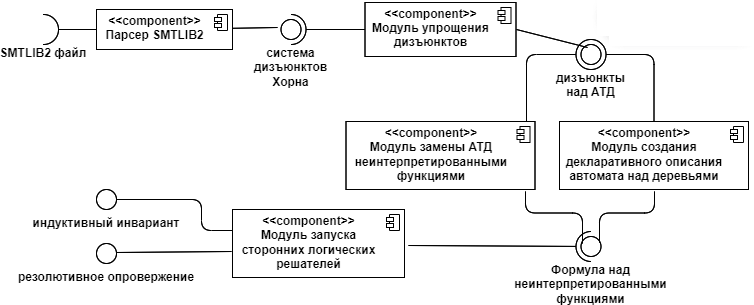
\includegraphics[width=\textwidth]{Dissertation/images/arch.png}
    \caption{Architecture of \theringen{}}
    \label{fig:ringen-arch}
\end{figure}


\textbf{\theringen{}.}\label{sec:ringen-pure}
% Итак, подход, представленный в главе~\ref{ch:fmf}, реализован автором данного исследования в рамках Хорн-решателя \theringen{}.
% Как сам подход, так и его реализация подразумевают использование стороннего SMT-решателя $\verifier$ для теории неинтерпретированных функций с кванторами, поэтому предлагаемая реализация в дальнейшем будет обозначаться $\ringen{\verifier}$.
% В частности, в качестве решателя $\verifier$ в экспериментах используются инструмент \vampire{}~\cite{reger2017instantiation} и SMT-решатель \cvc{}.
% Инструмент \vampire{} использует портфолио- подход~\cite{reger2014challenges}, то есть перебирает различные техники проверки выполнимости формул, построенные на насыщении системы~\cite{kovacs2013first} или на поиске конечных моделей~\cite{10.1007/978-3-319-40970-2_20}.
% Инструмент \cvc{} используется в режиме построения конечных моделей\footnote{с опцией \texttt{-{}-finite-model-find}}~\cite{reynolds2013finite}.
% Оба инструмента позволяют как доказывать безопасность системы, так и находить контрпримеры.
Hence, we implemented the approach presented in Chapter~\ref{ch:fmf} within the Horn solver \theringen{}. 
Both the approach itself and its implementation involve the use of an external SMT solver $\verifier$ for the theory of uninterpreted functions with quantifiers, therefore the proposed implementation will be further denoted as $\ringen{\verifier}$.
Specifically, \vampire{}~\cite{reger2017instantiation} and the SMT solver \cvc{} are used as the $\verifier$ in the experiments.
\vampire{} uses a portfolio-based approach~\cite{reger2014challenges}, that is, it iterates through various formula satisfiability checking techniques, based on saturation of the system~\cite{kovacs2013first} or finite model finding~\cite{10.1007/978-3-319-40970-2_20}.
\cvc{} is used in the finite model finding mode\footnote{with the \texttt{-{}-finite-model-find} option}~\cite{reynolds2013finite}.
Both tools allow for both proving the safety of the system and finding counterexamples.

\textbf{\ringenSync{}.}
% Этот подход представленный в  главе~\ref{ch:SyncReg}, реализован как надстройка над $\ringen{\verifier}$.
% В качестве стороннего решателя $\verifier$ в экспериментах использовался \cvc{}, поскольку \ringenSync{} порождает символы с большой арностью, которые не поддерживаются инструментом \vampire{}\footnote{\url{https://github.com/vprover/vampire/issues/348\#issuecomment-1091782513}}.
% Эта реализация в дальнейшем будет обозначаться \ringenSync{}\footnote{\url{https://github.com/Columpio/RInGen/releases/tag/ringen-tta}}.
The approach presented in Chapter~\ref{ch:SyncReg} has been implemented as an extension of $\ringen{\verifier}$.
In the experiments, \cvc{} was used as the external solver $\verifier$, as \ringenSync{} generates symbols with high arity, which are not supported by \vampire{}\footnote{\url{https://github.com/vprover/vampire/issues/348\#issuecomment-1091782513}}.
This implementation will be hereinafter referred to as \ringenSync{}\footnote{\url{https://github.com/Columpio/RInGen/releases/tag/ringen-tta}}.

\textbf{\theringenCICI{}.}
% Данный подход, представленный  в главе~\ref{ch:cici}, реализован в рамках кодовой базы Хорн-решателей \racer{}~\cite{10.1145/3498722} (развитие Хорн-решателя \spacer{}~\cite{komuravelli2016smt}, реализованное в логическом решателе \zprover{}\footnote{\url{https://github.com/Columpio/z3/tree/racer-solver-interaction}}) и Хорн-решателя $\ringen{\verifier{}}$\footnote{\url{https://github.com/Columpio/RInGen/releases/tag/chccomp22}}, описанного выше.
% Эта реализация в дальнейшем будет обозначаться $\ringenCICI{\verifier{}}$. Далее описаны обе части этой реализации в Хорн-решателях \racer{} и $\ringen{\verifier{}}$, соответственно, которые далее называются \emph{базовыми} относительно инструмента $\ringenCICI{\verifier{}}$.
The approach presented in Chapter~\ref{ch:cici} has been implemented within the codebase of the Horn solvers \racer{}\cite{10.1145/3498722} (a development of the Horn solver \spacer{}\cite{komuravelli2016smt}, implemented in the logical solver \zprover{}\footnote{\url{https://github.com/Columpio/z3/tree/racer-solver-interaction}}) and the Horn solver $\ringen{\verifier{}}$\footnote{\url{https://github.com/Columpio/RInGen/releases/tag/chccomp22}}, which was described earlier.
This implementation will be referred to as $\ringenCICI{\verifier{}}$ in the future. The following describes both parts of this implementation in the Horn solvers \racer{} and $\ringen{\verifier{}}$, respectively, which are subsequently referred to as \emph{basic} relative to the tool $\ringenCICI{\verifier{}}$.


\paragraph{\zprover{}/\racer{}.}
% Хорн-решатель \racer{} разработан Ари Гурфинкелем (Arie Gurfinkel) и Хари Говинд Ведирамана Кришнаном (Hari Govind Vediramana Krishnan) из университета Ватерлоо.
% Инструмент \racer{} основан на подходе, называемом достижимость, направляемая свойством (Property-Directed Reachability, PDR)~\cite{komuravelli2016smt}, который можно рассматривать как сложный экземпляр \cegar{}.
% PDR строит абстрактные состояния в виде конъюнкции формул (называемых \emph{леммами}) на различных \emph{уровнях} путём итеративного увеличения уровня в цикле.
% При этом поддерживаются следующие возможности: если набор лемм $\{\phi_i\}$ был построен на уровне $n$, то $\bigwedge_i \phi_i$ аппроксимирует сверху все состояния, достижимые менее чем за $n$ шагов перехода, и аппроксимирует снизу свойство безопасности.
% Таким образом, леммы в PDR выполняют требование абстракции в процедуре \RunBlackBox{} (алгоритм~\ref{code:runblackbox}).
% Хорн-решатель \racer{} был модифицирован в рамках данного диссертационного исследования таким образом, чтобы в конце каждой итерации набор лемм последнего уровня асинхронно передавался новому процессу инструмента $\ringen{\verifier{}}$.
The \racer{} Horn solver was developed by Arie Gurfinkel and Hari Govind Vediramana Krishnan from the University of Waterloo. It is based on an approach called Property-Directed Reachability (PDR)~\cite{komuravelli2016smt}, which can be considered a complex instance of \cegar{}. PDR builds abstract states in the form of conjunctions of formulas (referred to as \emph{lemmas}) at various \emph{levels} by iteratively increasing the level in a loop. The following capabilities are supported: if a set of lemmas $\{\phi_i\}$ was constructed at level $n$, then $\bigwedge_i \phi_i$ overapproximates all states reachable in less than $n$ transition steps, and under-approximates the safety property. Thus, in PDR, lemmas fulfill the requirement of abstraction in the \RunBlackBox{} procedure (algorithm~\ref{code:runblackbox}). As part of this thesis, \racer{} was modified to asynchronously pass the set of lemmas from the last level to a new process of $\ringen{\verifier{}}$ at the end of each iteration.


\paragraph{$\ringen{\verifier{}}$.}
% Процедура \RunBlackBox{} (алгоритм~\ref{code:runblackbox}) реализована на основе инструмента  $\ringen{\verifier{}}$. Было выполнено  следующее обобщение в процедуре $\substituteLemmas(\prog, a)$ (см.~\autoref{sec:subst_lemmas}).
% Конъюнктивная форма лемм инструмента \racer{} используется для вывода инвариантов более общего вида:
% $\bigwedge_i(\phi_i(\overline{x})\,\lor\,\overline{x}\!\in\!L_i)$.
% Так, имея $a(P) = \bigwedge_i \phi_i$,
% мы заменяем все атомы $P(\overline{t})$ на \emph{конъюнкцию дизъюнкций} $\bigwedge_i (\phi_i(\overline{t})\lor L_i(\overline{t}))$ с новыми предикатными символами $L_i$.
% Это позволяет выводить более общие инварианты, чем инварианты из объединения классов $\elemclass{}$ и $\abstrDomain$ (см. определение~\ref{def:combined-class}), которое состоит только из формул вида $\phi(\overline{x})\,\lor\,\overline{x}\!\in\!L$.
The \RunBlackBox{} procedure (algorithm~\ref{code:runblackbox}) is implemented based on the $\ringen{\verifier{}}$. The following generalization was carried out in the $\substituteLemmas(\prog, a)$ procedure (see~\autoref{sec:subst_lemmas}). The conjunctive form of lemmas from \racer{} is used to infer more general invariants: $\bigwedge_i(\phi_i(\overline{x})\,\lor\,\overline{x}\!\in\!L_i)$. Hence, given $a(P) = \bigwedge_i \phi_i$, we replace all atoms $P(\overline{t})$ with a \emph{conjunction of disjunctions} $\bigwedge_i (\phi_i(\overline{t})\lor L_i(\overline{t}))$ with new predicate symbols $L_i$. This allows inferring more general invariants than those from the union of $\elemclass{}$ and $\abstrDomain$ (see Definition~\ref{def:combined-class}), which consists only of formulas of the form $\phi(\overline{x})\,\lor\,\overline{x}\!\in\!L$.

% После преобразований модифицированный $\ringen{\verifier{}}$ вызывает сторонний решатель $\verifier{}$ с ограничением по времени в 30 секунд.
% Затем его результаты передаются обратно в Хорн-решатель \racer{}, где они асинхронно обрабатываются.
% Кроме того, реализация не выполняет дорогостоящее преобразование в КНФ из алгоритма~\ref{code:residual-chc}, так как реализация $\ringen{\verifier{}}$ позволяет принимать на вход дизъюнкты Хорна в произвольном виде, поскольку он полагается на сторонний решатель $\verifier{}$ с полной поддержкой логики первого порядка.
After the transformations, the modified $\ringen{\verifier{}}$ calls the external solver $\verifier{}$ with a time limit of 30 seconds. Then its results are passed back to \racer{}, where they are processed asynchronously. Moreover, the implementation does not perform the costly transformation into CNF from algorithm~\ref{code:residual-chc}, as the $\ringen{\verifier{}}$ implementation allows inputting Horn clauses in arbitrary form, since it relies on the external solver $\verifier{}$ with full first-order logic support.

\section{Related Work}\label{ch:relatedWork}

% Раздел~\cref{sec:relatedWork/hornSolvers} данной главы посвящен сравнению предложенных методов решения систем дизъюнктов Хорна с алгебраическими типами данных и существующих методов, реализованных в таких инструментах, как \spacer{}, \racer{}, \eldarica{}, \vericat{}, \hoice{} и \rchc{}. Данные инструменты были отобраны по следующему принципу: инструменты, поддерживающие системы дизъюнктов Хорна над алгебраическими типами данных, которые проверяют как выполнимость, так и не выполнимость этих систем. Так, например, не рассматривались инструменты, решающие родственную проблему автоматизации индукции для теорем с алгебраическими типами данных, такие как, например, \cvc{} в режиме индукции~\cite{reynolds2015induction} (см. предыдущий раздел), \textsc{AdtInd}~\cite{10.1007/978-3-030-30048-7_35} и пр., поскольку они не принимают на вход системы дизъюнктов Хорна. Также не рассматривались инструменты логического программирование (такие, как \textsc{Prolog}~\cite{ClocksinMellish03}), поскольку они позволяют проверять только невыполнимость систем дизъюнктов Хорна и ничего не говорят об их выполнимости.
This section of this chapter is dedicated to the comparison of proposed methods for solving Horn clause systems with algebraic data types and existing methods, implemented in tools such as \spacer{}, \racer{}, \eldarica{}, \vericat{}, \hoice{}, and \rchc{}. We selected only the tools supporting Horn clause systems over algebraic data types that verify both the satisfiability and unsatisfiability of these systems. For instance, tools addressing the related problem of automating induction for theorems with algebraic data types, such as, for example, \cvc{} in induction mode~\cite{reynolds2015induction}, \textsc{AdtInd}~\cite{10.1007/978-3-030-30048-7_35} and others were not considered, as they do not accept Horn clause systems as input. Also, logic programming tools (such as \textsc{Prolog}~\cite{ClocksinMellish03}) were not considered because they only check the unsatisfiability of Horn clause systems and say nothing about their satisfiability.

\begin{table} [htbp]
    \centering
    \begin{threeparttable}% выравнивание подписи по границам таблицы
        \caption{Comparison of Horn solvers with ADT support}\label{tab:hornSolvers}%
        \begin{tabular}{| m{41mm} || x{29mm} | x{28mm} | x{27mm} | x{26mm} |}
            \hline
            \hline
Tool & Invariant class & Method & Returns the invariant & Fully automatic\\\hline\hline
\spacer{} & \elemclass{} & \pdr{} & Yes & Yes\\
\racer{} & \catelemclass{} & \pdr{} & No & No\\
\eldarica{} & \sizeelemclass{} & \cegar{} & Yes & Yes\\
\vericat{} & -- & Transf. & No & Yes\\
\hoice{} & \elemclass{} & \ice{} & Yes & Yes\\
\rchc{}  & \syncRegFlatClass{} & \ice{} & Yes & Yes\\\hline
\ringenShort{\cvc} & \regclass{} & Transf. + \fmf{} & Yes & Yes\\
\ringenShort{\vampire} & -- & Transf. + Saturation & No & Yes\\
\ringenSyncShort{} & \syncRegFullClass{} & Transf. + \fmf{} & Yes & Yes\\
\ringenCICIShort{\cvc} & \regelemclass{} & \ourCEGAR{} & Yes & Yes\\
\ringenCICIShort{\vampire} & -- & \ourCEGAR{} & No & Yes\\
            \hline
            \hline
        \end{tabular}
    \end{threeparttable}
\end{table}

% В таблице~\cref{tab:hornSolvers} представлены результаты сравнения работе Хорн-решателей~--- существующих (верхний блок) и предложенных в данной (нижний блок). Предложенные Хорн-решатели описаны в предыдущей главе~\ref{ch:evaluation}, реализуемые ими методы описаны в главах~\ref{ch:fmf},~\ref{ch:SyncReg} и~\ref{ch:cici} данной работы. В таблице, для краткости, название \theringen{} сокращено до \theringenShort{}, так, например, Хорн-решатель \ringenSync{} в таблице представлен как \ringenSyncShort{}. Под словом <<Transf.>> имеется в виду, что инструмент построен на применении нетривиальных трансформаций к системе; аббревиатура <<FMF>> обозначает применение автоматического поиска конечных моделей (<<finite-model finding>>, см., например,~\cite{10.1007/978-3-319-40970-2_20,reynolds2013finite}); прочерк в столбце <<Класс инвариантов>> означает следующее: несмотря на то, что при выполнимости системы вывод инструмента неявно кодирует её индуктивный инвариант, не существует всюду останавливающейся процедуры, позволяющей этот вывод проверить. Остальные обозначения поясняются в подразделах, посвящённых соответствующим инструментам.
Table~\cref{tab:hornSolvers} presents the comparison of Horn solvers: existing ones (upper block) and those proposed in this work (lower block). The proposed Horn solvers are described in Chapter~\ref{ch:evaluation}, and the methods they implement are described in Chapters~\ref{ch:fmf},~~\ref{ch:SyncReg}, and~~\ref{ch:cici} of this work. In the table, for brevity, the name \theringen{} is abbreviated to \theringenShort{}, so for example, the Horn solver \ringenSync{} in the table is represented as \ringenSyncShort{}. The word ``Transf.'' indicates that the tool is built using non-trivial transformations of the system; ``FMF'' denotes the application of automatic finite-model finding (e.g., see~\cite{10.1007/978-3-319-40970-2_20,reynolds2013finite}); a dash in the ``Class of Invariants'' column means the following: although when the system is satisfiable, the output of the tool implicitly encodes its inductive invariant, there is no everywhere-halting procedure that allows this output to be checked. The other designations are explained in the subsections dedicated to the corresponding tools.

% Большинство рассмотренных инструментов отличаются классами, в которых они ищут индуктивные инварианты. Сравнение самих классов инвариантов было приведено в главе~\cref{ch:comparison}. В контексте сопоставления инструментов сравнение их классов инвариантов важно по следующей причине: если инструмент выводит инварианты в некотором классе, то проблема невыразительности этого класса (невозможность выразить определённые типы отношений) превращается в проблему незавершаемости этого инструмента. Иными словами, поскольку ни один из существующих инструментов не проверяет, существует ли \emph{вообще} инвариант для данной системы дизъюнктов Хорна в его классе\footnote{С одной стороны, эта задача по сложности сравнима с самой задачей верификации, с другой же стороны до сих пор ей были посвящены лишь отдельные работы (см., например,~\cite{10.1145/3022187,10.1145/2837614.2837640})}, то в случае отсутствия такового инструмент не будет завершаться.
Most of the tools examined differ in the classes in which they seek inductive invariants. A comparison of these classes of invariants was given in Chapter~\cref{ch:comparison}. This comparison is important for comparing tools for the following reason: if a tool outputs invariants in a certain class, then the problem of expressiveness of this class (the inability to express certain types of relations) becomes the problem of non-termination of this tool. In other words, since none of the existing tools check whether there is an invariant \emph{at all} for a given Horn clause system in its class\footnote{On the one hand, this task is as complex as the verification task itself; on the other hand, so far only a few studies have been dedicated to it (see, for example,~\cite{10.1145/3022187,10.1145/2837614.2837640})}, then in the absence of such, the tool will not terminate.

% Далее приведено краткое сравнительное описание существующих инструментов.
Further on, we provide a short comparartive descrition of the existing tools.

% \paragraph{Инструмент \spacer{}~\cite{komuravelli2016smt}} строит элементарные модели (класс \elemclass{} из раздела~\cref{sec:elem-def}). Этот инструмент создан на основе классической разрешающей процедуры для АТД, а также процедуры интерполяции и устранения кванторов~\cite{bjorner2015playing}. Ядром инструмента является подход \spacer{}, который основан на технике, называемой \emph{достижимость, направляемая свойством} \foreignlanguage{english}{(property-directed reachability, \pdr{})}, которая равномерно распределяет время анализа между поиском контрпримеров и построением безопасного индуктивного инварианта, распространяя информацию о достижимости небезопасных свойств и частичные леммы о безопасности. Инструмент позволяет выводить инварианты в комбинации алгебраических и других типов данных, возвращает проверяемые сертификаты. Подход, используемый в инструменте, корректен и полон. Недостатком инструмента является то, что он выражает инварианты в языке ограничений, а потому часто не завершается на проблемах с АТД.
\paragraph{The \spacer{} tool~\cite{komuravelli2016smt}} constructs elementary models (the \elemclass{} class). This tool is based on a classic satisfiability procedure for ADTs, as well as interpolation and quantifier elimination procedures~\cite{bjorner2015playing}. At its core, the tool employs the \spacer{} approach, which is based on a technique called \emph{property-directed reachability} (\pdr{}), evenly distributing analysis time between counterexample search and safe inductive invariant construction, propagating information about reachability of unsafe properties and partial safety lemmas. The tool allows for the output of invariants in a combination of algebraic and other data types, and returns verifiable certificates. The approach used in the tool is both sound and complete. A drawback of the tool is that it expresses invariants in the constraint language, and therefore often does not terminate on problems with ADTs.

% \paragraph{Инструмент \racer{}~\cite{10.1145/3498722}} является развитием инструмента \spacer{}, позволяя выводить инварианты в языке ограничений, расширенном катаморфизмами. Этот язык ограничений обозначен в таблице~\ref{tab:hornSolvers} как \catelemclass{}. \racer{} также наследует все достоинства подхода \spacer{}. Недостатком подхода является то, что он не полностью автоматический, поскольку требует вручную описывать катаморфизмы, что может быть затруднительно на практике, поскольку по заданной проблеме бывает сложно понять, какие катаморфизмы потребуются для её инварианта. Недостатком самого инструмента является то, что он не возвращает какие-либо проверяемые сертификаты с катаморфизмами.

\paragraph{The \racer{} tool~\cite{10.1145/3498722}} is an evolution of the \spacer{} tool, allowing for the output of invariants in the constraint language expanded with catamorphisms. This constraint language is denoted in table~\ref{tab:hornSolvers} as \catelemclass{}. \racer{} also inherits all the advantages of the \spacer{} approach. A drawback of the approach is that it's not fully automatic, as it requires manually describing catamorphisms, which can be challenging in practice because it can be difficult to understand which catamorphisms will be required for the invariant based on the given problem. A drawback of the tool itself is that it does not return any verifiable certificates with catamorphisms.

% \paragraph{Инструмент \eldarica{}~\cite{8603013}} строит модели с ограничениями размера термов, которые вычисляют общее количество вхождений конструкторов (\sizeelemclass{} из раздела~\cref{sec:sizeelem-def}). Это расширение весьма ограниченно увеличивает выразительность языка ограничений, поскольку введённая функция считает количество всех конструкторов одновременно, поэтому с её помощью невозможно выразить многие свойства, например, ограничение на высоту дерева. Инструмент \eldarica{} использует подход \cegar{} с абстракцией предикатов и встроенный SMT-решатель \princess{}~\cite{princess}, который предоставляет разрешающую процедуру, а также процедуру интерполяции для АТД с ограничениями на размер термов. Эти процедуры построены на сведении данной теории к комбинации теорий неинтерпретируемых функций и линейной арифметики~\cite{hojjat2017deciding}.
\paragraph{The \eldarica{} tool~\cite{8603013}} constructs models with term size constraints, which calculate the total number of constructor occurrences (the \sizeelemclass{} class). This extension only marginally enhances the expressiveness of the constraint language, as the introduced function counts all constructors at once, thus it cannot express many properties, such as a restriction on tree height. The \eldarica{} tool employs the \cegar{} approach with predicate abstraction and an embedded SMT solver \princess{}\cite{princess}, which provides a resolution procedure, as well as an interpolation procedure for algebraic data types with term size constraints. These procedures are built on the reduction of this theory to a combination of theories of uninterpreted functions and linear arithmetic\cite{hojjat2017deciding}.

% \paragraph{Инструмент \vericat{}~\cite{10.1093/logcom/exab090,pettorossi_proietti_2022,10.1007/978-3-030-51074-9_6,angelis_fioravanti_pettorossi_proietti_2018}} обрабатывает условия проверки над теориями линейной арифметики и АТД и полностью устраняет АТД из исходной системы дизъюнктов путём сворачивания (fold), разворачивания (unfold), введения новых дизъюнктов и других трансформаций. После работы инструмента получается система дизъюнктов Хорна без АТД, на которой может быть запущен любой эффективный Хорн-решатель, например, \spacer{} или \eldarica{}. Основным достоинством подхода является тот факт, что он рассчитан на работу с проблемами, где алгебраические типы данных комбинированы с другими теориями. Основные недостатки подхода заключаются в следующем: сам процесс трансформации может также не завершаться, кроме этого из-за трансформации невозможно восстановить инвариант исходной системы, т.\:е. инструмент не возвращает проверяемого сертификата.
\paragraph{The \vericat{} tool~\cite{10.1093/logcom/exab090,pettorossi_proietti_2022,10.1007/978-3-030-51074-9_6,angelis_fioravanti_pettorossi_proietti_2018}} processes verification conditions over theories of linear arithmetic and ADTs and completely eliminates ADTs from the original system of Horn clauses by folding, unfolding, introducing new clauses, and other transformations. It produces a Horn clause system without ADTs, on which any efficient Horn solver, such as \spacer{} or \eldarica{}, can be run. The main advantage of this approach is that it is designed to work with problems where algebraic data types are combined with other theories. The main drawbacks of the approach are as follows: the transformation process itself may also not terminate, and due to the transformation, it is impossible to recover the invariant of the original system, i.e., the tool does not return a verifiable certificate.

% \paragraph{Инструмент \hoice{}~\cite{10.1007/978-3-030-02768-1_8}} строит элементарные инварианты с помощью подхода, основанного на машинном обучении, \ice{}~\cite{10.1007/978-3-319-08867-9_5}. Его достоинством является возможность выводить инварианты в комбинации АТД с другими теориями, а также корректность и полнота, и, наконец, способность возвращать проверяемые сертификаты корректности. Его недостатком является то, что он выводит инварианты в невыразительном языке ограничений, а потому часто не завершается.
\paragraph{The \hoice{} tool~\cite{10.1007/978-3-030-02768-1_8}} constructs elementary invariants using an approach based on machine learning, \ice{}~\cite{10.1007/978-3-319-08867-9_5}. Its advantages include the ability to infer invariants for combinations of ADTs with other theories, as well as correctness and soundness, and finally, the ability to return verifiable correctness certificates. Its disadvantage is that it produces invariants in an expressive constraint language, and thus often does not terminate.

% \paragraph{Инструмент \rchc{}~\cite{haude2020,losekoot_et_al:LIPIcs.FSCD.2023.7},}также как и \hoice{}, использует подход \ice{}; \rchc{} основан на машинном обучении, однако выражает индуктивные инварианты программ над АТД при помощи \emph{автоматов над деревьями}~\cite{tata}. Но из-за сложностей с выражением кортежей термов автоматами, описанных в разделе~\ref{sec:comparison/undef-in-sync}, подход часто оказывается неприменим для простейших примеров, где существуют классические символьные инварианты. 
\paragraph{The \rchc{} tool~\cite{haude2020,losekoot_et_al:LIPIcs.FSCD.2023.7}} also uses the \ice{} approach; it is based on machine learning, but expresses inductive invariants of programs over ADTs using \emph{tree automata}~\cite{tata}. However, due to the complexities of expressing tuples of terms with automata, described in Section~\ref{sec:comparison/undef-in-sync}, the approach often proves inapplicable for even the simplest examples where classical symbolic invariants exist.

% \paragraph{Выводы.} Подводя итоги сравнения вышеозначенных инструментов и методов, можно сказать следующее. По сравнении с методом инструмента \rchc{} предложенные в данной диссертационной работе подходы являются альтернативными способами вывода регулярных инвариантов и их надклассов. Поэтому они могут быть совмещены с подходом инструмента \rchc{}, чтобы быстрее сходиться к индуктивному инварианту системы, если он существует. В сравнении с методами остальных существующих инструментов, предложенные подходы позволяют выводить инварианты в независимых классах регулярных инвариантов. Поэтому применение предложенных методов совместно с существующими позволит решать больше различных типов задач.
\paragraph{Conclusions.} Summarizing the comparison, the following can be said. Compared with the method of \rchc{}, the approaches proposed in this thesis provide alternative ways of inferring regular invariants and their superclasses. Therefore, they can be combined with the \rchc{} approach to converge faster to the inductive invariant of the system, if it exists. Compared with the methods of the remaining existing tools, the proposed approaches allow inferring invariants in independent classes of regular invariants. Therefore, the application of the proposed methods in conjunction with existing ones will solve a wider variety of problems.

\section{Evaluation}
\subsection{Tool Selection}
% В качестве инструментов для сравнения были выбраны \racer{}~\cite{10.1145/3498722} и \eldarica{}~\cite{8603013}~--- Хорн-решатели с поддержкой алгебраических типов данных, лидирующие на соревнованиях \chccomp{}~\cite{De_Angelis_2022}.
% Также  были выбраны инструменты \cvcind{} (\cvc{} в режиме индукции)~\cite{reynolds2015induction} и \vericat{}~\cite{10.1093/logcom/exab090}.
% Несмотря на то, что эти инструменты не строят индуктивные инварианты \emph{явно}, из-за чего невозможно проверить их корректность, их запуск на эквивалентном бенчмарке добавлен в экспериментальное сравнение, поскольку они решают родственную задачу.
We have selected the \racer{}~\cite{10.1145/3498722} and \eldarica{}~\cite{8603013} tools for compassion, which are Horn solvers with support for algebraic data types leading in the \chccomp{} competition~\cite{De_Angelis_2022}. We also selected \cvcind{} (\cvc{} in induction mode)~\cite{reynolds2015induction} and \vericat{}~\cite{10.1093/logcom/exab090}. Although these tools do not construct inductive invariants explicitly, making it impossible to check their correctness, their launch on an equivalent benchmark is added to the experimental comparison as they solve a related task.


% В представленных здесь экспериментах не участвовал Хорн-решатель \hoice{}~\cite{10.1007/978-3-030-02768-1_8}, поскольку он работает не быстрее \racer{}~\cite{10.1145/3498722} и при этом ищет инварианты в том же классе инвариантов \elemclass{}.
% Другой известный Хорн-решатель \rchc{}~\cite{haude2020} не участвовал в экспериментах, поскольку он работает нестабильно и  часто либо завершается с ошибкой, либо возвращает некорректные результаты.

\subsection{Benchmark Suite}
% Эксперименты проводились на наборе данных \emph{TIP} (Tons of Inductive Problems)~\cite{claessen2015tip}, тестового набора с трека соревнования \chccomp{} 2022\footnote{\url{https://github.com/chc-comp/ringen-adt-benchmarks}}, посвящённого алгебраическим типам данных. Набор \emph{TIP} состоит из 454 систем дизъюнктов Хорна, полученных из \haskell{}-программ с АТД и рекурсией.
% В тестовом наборе встречаются следующие алгебраические типы данных~--- списки, очереди, регулярные выражения и целые числа Пеано.

The experiments were conducted on the TIP (Tons of Inductive Problems) benchmark suite~\cite{claessen2015tip}, the test set from the 2022 \chccomp{} competition track\footnote{\url{https://github.com/chc-comp/ringen-adt-benchmarks}}, dedicated to algebraic data types. The TIP set consists of 454 Horn clause systems derived from Haskell programs with ADTs and recursion. The test set includes the following algebraic data types: lists, queues, regular expressions, and Peano integers.

\subsection{Setup}
% Эксперименты проводились на платформе StarExec~\cite{stump2014starexec}, имеющей кластер машин с Intel(R) Xeon(R) CPU E5-2609 0 @ 2.40GHz и Red Hat Enterprise Linux~7\footnote{\url{https://www.starexec.org/starexec/public/machine-specs.txt}}, с ограничением на процессорное время работы каждого инструмента на каждом тесте в 600~секунд и с ограничением по памяти в 16~ГБ.
The experiments were conducted on the StarExec platform~\cite{stump2014starexec}, which has a cluster of machines with Intel(R) Xeon(R) CPU E5-2609 0 @ 2.40GHz and Red Hat Enterprise Linux~7\footnote{\url{https://www.starexec.org/starexec/public/machine-specs.txt}}, with a limit on the CPU runtime for each tool on each test of 600 seconds and a memory limit of 16 GB.

\subsection{Research Questions}

% Для постановки экспериментов были поставлены следующие исследовательские вопросы.
We have formulated the following research questions to guide the experimental setup.
\begin{resquest}[Number of solutions]\label{rq:conv}
$ $

% Поскольку основная цель данной работы~--- предложить подходы, позволяющие проверять выполнимость б\textit{о}льшего числа систем, чем аналоги, путём вывода индуктивных инвариантов, ключевыми являются следующие вопросы.
\begin{itemize}
    % \item Позволяют ли предложенные подходы проверять выполнимость б\textit{о}льшего числа систем, чем подходы, строящие классические символьные инварианты?
    % \item Позволяют ли предложенные подходы проверять выполнимость систем, у которых существуют классические инварианты?
    \item Do the proposed methods allow for the verification of more systems than approaches that construct classical symbolic invariants?
    \item Do the proposed methods allow for the verification of systems that have classical invariants?

\end{itemize}
\end{resquest}

\begin{resquest}[Performance]\label{rq:perf}
$ $

\begin{itemize}
    % \item Какова производительность инструментов \theringen{} и \ringenSync{} на проблемах, которые смогли решить они, а также существующие инструменты?
    % \item Коллаборативный вывод в \theringenCICI{} может потребовать параллельного запуска нескольких экземпляров оракула. Каково влияние параллельного запуска на производительность?
    \item What is the performance of \theringen{} and \ringenSync{} on problems that they, as well as existing tools, were able to solve?
    \item Collaborative inference in \theringenCICI{} may require parallel launching of multiple oracle instances. What is the impact of parallel launching on performance?

\end{itemize}
\end{resquest}

\begin{resquest}[Significance of the inductive invariant class]\label{rq:char}
% Коллаборативный вывод, реализованный в \theringenCICI{}, теоретически позволяет не только выводить инварианты в большем классе, но и ускорять сходимость поиска классических символьных инвариантов. Какова при этом доля классических символьных инвариантов на всех уникально решённых инструментом \theringenCICI{} проблемах?
Collaborative inference, implemented in \theringenCICI{}, theoretically allows not only to infer invariants in a larger class but also to accelerate the convergence of the search for classical symbolic invariants. What is the share of classical symbolic invariants in all uniquely solved problems by \theringenCICI{}?
\end{resquest}

\section{Results}



\subsection{Number of Solutions}

% Количество проблем из тестового набора, решённых существующими и предложенными инструментами, представлено в таблице~\ref{table:eval-all}.
The number of problems from the benchmark suite solved by the existing and proposed instruments is presented in Table~\ref{table:eval-all}.
\begin{table}[t]
    \caption{Results. SAT indicates that the system is safe (there is an inductive invariant), UNSAT indicates that the system is unsafe.}
    \label{table:eval-all}
    \small
    \centering
    \begin{tabular}{ |l|c|c| }
    \hline
    Tool & SAT & UNSAT\\\hline
    \cvcind{} & 0 & 13\\
    \eldarica{} & 46 & 12\\
    \racer{} & 26 & 22\\
    \ringen{\cvc{}} & 25 & 21\\
    \ringen{\vampire{}} & 135 & 46\\
    \ringenCICI{\cvc{}} & 117 & 19\\
    \ringenCICI{\vampire{}} & 189 & 28\\
    \ringenSync{} & 43 & 21\\
    \vericat{} & 16 & 10\\
    \hline
    \end{tabular}
\end{table}

%\subsubsection{\theringen{}.}

% \textbf{\theringen{}}. На всех 12 проблемах, на которых инструмент \eldarica{} вернул ответ <<UNSAT>>, инструмент \theringen{} завершился с тем же результатом и он нашёл больше контрпримеров.
% Инструменты \ringen{\cvc{}}, \ringen{\vampire{}} и \racer{} нашли контрпримеры для 21, 46 и 22 систем дизъюнктов соответственно. Большинство из этих систем совпадает, хотя некоторые из них уникальны для каждого инструмента.
% Инструмент \ringen{\vampire{}} построил существенно больше <<UNSAT> результатов, чем другие инструменты, поскольку в инструменте \vampire{} реализована эффективная процедура вывода опровержений.
% Тем самым, несмотря на то, что предложенные алгоритмы спроектированы для поиска большего числа индуктивных инвариантов, они также позволяют находить уникальные контрпримеры.
% Далее, инструмент \eldarica{} нашёл 46 инвариантов в противовес 25 и 135 инвариантам, найденным \ringen{\cvc{}} и \ringen{\vampire{}}.
% Из них \eldarica{} решила 25 уникальных (не решённых \ringen{\cvc{}}) задач, каждая из которых является формулировкой некоторого свойства порядковых предикатов ($ <, \le,>, \ge $) на числах Пеано.
% Эти проблемы легко решаются инструментом \eldarica{}, поскольку порядковые предикаты сами по себе включены в домен верификации \sizeelemclass{} на уровне примитивов.
% Тем не менее инструмент \ringen{\cvc{}} решил 13 уникальных (не решённых \eldarica{}) проблем, чьи инварианты не представимы в домене верификации инструмента \eldarica{}.
% Эффективность реализованного в инструменте \theringen{} подхода существенно зависит от используемого стороннего решателя, как видно из того, что инструмент \ringen{\vampire{}} вывел более чем в 5 раз больше инвариантов, чем инструмент \ringen{\cvc{}}.
\textbf{\theringen{}}. On all 12 problems where \eldarica{} returned UNSAT, \theringen{} terminated with the same result, and it found more counterexamples.
The \ringen{\cvc{}}, \ringen{\vampire{}}, and \racer{} found counterexamples for 21, 46, and 22 clause systems, respectively. Most of these systems are the same, although some are unique to each tool.
\ringen{\vampire{}} constructed significantly more UNSAT results than other tools, as \vampire{} implements an efficient refutation inference procedure.
Therefore, even though the proposed algorithms are designed to search for more inductive invariants, they also allow for finding unique counterexamples.
Next, \eldarica{} found 46 invariants in contrast to 25 and 135 invariants found by \ringen{\cvc{}} and \ringen{\vampire{}}.
Out of these, \eldarica{} solved 25 unique (not solved by \ringen{\cvc{}}) tasks, each of which is a formulation of some property of ordinal predicates ($ <, \le,>, \ge $) on Peano numbers.
These problems are easily solved by \eldarica{}, as ordinal predicates are themselves included in the \sizeelemclass{} verification domain at the primitive level.
However, \ringen{\cvc{}} solved 13 unique (not solved by \eldarica{}) problems, which invariants are not expressible in the verification domain of the \eldarica{}.
The effectiveness of the approach implemented in the \theringen{} heavily depends on the external solver used, as evidenced by the fact that \ringen{\vampire{}} inferred more than 5 times more invariants than \ringen{\cvc{}}.


% \textbf{\ringenSync{}.} Данный инструмент завершился с ответом UNSAT на 21 проблеме, эти ответы в точности совпадают с 21 результатом инструмента \ringen{\cvc{}}, поскольку поиск контрпримеров инструмент \ringenSync{} наследует от последнего.
\textbf{\ringenSync{}.} This tool terminated with UNSAT on 21 problems, these results exactly match the 21 results of the \ringen{\cvc{}}, since \ringenSync{} inherits the counterexample search from the latter.

% Среди всех полученных инструментом \eldarica{} ответов SAT 38 были также получены инструментом \ringenSync{}.
% Большое количество пересечений с результатами инструмента \eldarica{} связано с тем, что \eldarica{} хорошо справляется с проблемами, которые кодируют порядок на числах Пеано, который также хорошо кодируется полносвёрточными синхронными автоматами над деревьями, используемыми в \ringenSync{}. \racer{} завершился с ответом SAT на 26 системах, 15 из которых пересекаются с ответами инструмента \ringenSync{}. Также инструмент \ringenSync{} вывел 4 уникальных инварианта. Несмотря на то, что теоретически выразительная сила полносвёрточных синхронных автоматов над деревьями, используемых в \ringenSync{}, должна давать большее число решений, инструменты поиска конечных моделей, которые \ringenSync{} использует в качестве бэкенда, не завершаются на проблемах с большим количеством кванторов и потому \ringenSync{} часто не завершается.
% Результаты не меняются при изменении бэкенда с \cvc{} на другие инструменты поиска конечных моделей и увеличении ограничения на время до 1200 секунд. Небольшое количество пересечений с инструментом \racer{} говорит о том, что хотя в теории класс элементарных инвариантов почти полностью содержится в классе синхронных регулярных инвариантов, на практике предложенный подход не позволяет эффективно выводить инварианты систем, у которых существуют элементарные инварианты.
Among all SAT results obtained by \eldarica{}, 38 were also obtained by \ringenSync{}.
The large overlap with the results of \eldarica{} is due to the fact that \eldarica{} deals well with problems encoding the order on Peano numbers, which are also well-encoded by the fully-convolutional synchronous tree automata used in \ringenSync{}. \racer{} concluded with a SAT result on 26 systems, 15 of which intersect with the results of \ringenSync{}. Additionally, \ringenSync{} inferred 4 unique invariants. Despite the theoretical expressive power of the fully-convolutional synchronous tree automata used in \ringenSync{}, which should yield a larger number of solutions, the finite model finding tools that \ringenSync{} uses as a backend do not terminate on problems with a large number of quantifiers, and therefore \ringenSync{} often does not terminate.
The results do not change when changing the backend from \cvc{} to other finite model finding tools and increasing the time limit to 1200 seconds. The small overlap with \racer{} suggests that although in theory the class of elementary invariants is almost fully contained in the class of synchronous regular invariants, in practice the proposed approach does not effectively infer invariants of systems that have elementary invariants.


% \textbf{\theringenCICI{}.} Инструмент \theringenCICI{} решил меньше \textit{небезопасных проблем}, чем лучший из базовых решателей: \theringenCICI{} получил 19 (с \cvc{}) и 28 (с \vampire{}) UNSAT результатов против 21 (с \cvc{}) и 46 (с \vampire{}) UNSAT результатов, полученных \theringen{}. Основная причина в том, что предложенный подход спроектирован для решения более сложной задачи вывода индуктивных инвариантов и не вносит изменения в работу базовых алгоритмов поиска контрпримеров. То есть, с нашим подходом могут быть интегрированы ортогональные усовершенствования поиска контрпримеров, например, предложенные в~\cite{blicha2022transition}. Таким образом, все контрпримеры, полученные \theringenCICI{}, получены непосредственно от одного из базовых решателей. Некоторые контрпримеры, которые находит инструмент \theringen{}, не были найдены \theringenCICI{}, поскольку он запускает \theringen{} с ограничением по времени в 30 секунд. 
\textbf{\theringenCICI{}.} \theringenCICI{} solved fewer \textit{unsafe problems} than the best of the basic solvers: \theringenCICI{} obtained 19 (with \cvc{}) and 28 (with \vampire{}) UNSAT results against 21 (with \cvc{}) and 46 (with \vampire{}) UNSAT results obtained by \theringen{}. The main reason is that the proposed approach is designed to solve the more complex task of inferring inductive invariants and does not change the operation of the basic counterexample finding algorithms. That is, our approach can be integrated with orthogonal improvements to counterexample search, for example, those proposed in~\cite{blicha2022transition}. Thus, all counterexamples obtained by \theringenCICI{} are directly obtained from one of the basic solvers. Some counterexamples found by \theringen{} were not found by \theringenCICI{}, as it runs \theringen{} with a time limit of 30 seconds.

% Важно отметить, что все 20 SAT и 15 UNSAT ответов, полученных \racer{}, также были получены и инструментом \theringenCICI{}, за исключением одного UNSAT ответа.
It is important to note that all 20 SAT and 15 UNSAT answers obtained by \racer{}, were also obtained by \theringenCICI{}, with the exception of one UNSAT answer.

% \textit{На безопасных проблемах} инструмент \theringenCICI{} превзошёл конкурирующие решатели: \ringenCICI{\cvc{}} получил 117 SAT ответов, когда как \racer{} получил 20 SAT ответов, а \ringen{\cvc{}}~--- 25, также \ringenCICI{\vampire{}} получил 189 SAT ответов, при 20 SAT ответах от \racer{} и 135 от \ringen{\vampire{}}. 
% Таким образом, \theringenCICI{} решает значительно больше SAT задач, чем базовые инструменты, работающие по отдельности: 117 против $20+25$ и 189 против $20+135$ для соответствующих бэкендов \cvc{} и \vampire{}.
% В частности, \ringenCICI{\cvc{}} решает 97 задач, не решённых \racer{} и 94 задачи, не решённые \ringen{\cvc{}}.
% \ringenCICI{\vampire{}} решает 169 задач, не решённых \racer{} и 60 задач, не решённых \ringen{\vampire{}}.
% Таким образом, коллаборативный метод вывода инвариантов позволяет установить выполнимость существенно больше числа систем, чем параллельный запуск базовых инструментов.
\textit{On safe problems}, \theringenCICI{} outperformed competitive solvers: \ringenCICI{\cvc{}} obtained 117 SAT responses, while \racer{} obtained 20 SAT responses, and \ringen{\cvc{}} 25. \ringenCICI{\vampire{}} obtained 189 SAT responses, with 20 SAT responses from \racer{} and 135 from \ringen{\vampire{}}.
Thus, \theringenCICI{} solves significantly more SAT tasks than the basic tools working separately: 117 versus $20+25$ and 189 versus $20+135$ for the respective \cvc{} and \vampire{} backends.
In particular, \ringenCICI{\cvc{}} solves 97 tasks not solved by \racer{} and 94 tasks not solved by \ringen{\cvc{}}.
\ringenCICI{\vampire{}} solves 169 tasks not solved by \racer{} and 60 tasks not solved by \ringen{\vampire{}}.
Therefore, the collaborative invariant inference method allows to establish the feasibility of significantly more systems than the parallel launch of basic tools.

% Однако есть проблемы, которые были решены базовыми решателями, но не предложенным инструментом. Инструмент \ringenCICI{\cvc{}} не решил 7 проблем, которые были успешно решены инструментом \ringen{\cvc{}}. Две из этих проблем могут быть решены предложенным инструментом, если увеличить 30-секундное ограничение по времени для работы бэкенда в \theringenCICI{}. Существующие методы предсказания времени проверки, такие как~\cite{10.1145/3121257.3121262}, могут быть применены для того, чтобы вообще избежать жесткого кодирования лимита времени. Остальные 5 проблем решаются мгновенно, однако их результаты не могут быть получены из межпроцессного взаимодействия в сделанной реализации. Причина заключается в том, что \racer{} тратит слишком большое время на решение SMT-ограничений, и поэтому не считывает результаты бэкенд-решателя. Этой технической проблемы можно избежать, если считывать результаты бэкенд-решателя в более частых контрольных точках, что, однако, приведёт к увеличению накладных расходов в инструменте. Аналогичная картина наблюдается и для \ringenCICI{\vampire{}}, который не смог решить 24 проблемы, решённые базовыми решателями. Только 8 из них не решены из-за низкого ограничения по времени для бэкенда, а остальные 16~--- из-за расхождения \racer{} в решении SMT-ограничений.
However, there are problems that were solved by the basic solvers but not by the proposed tool. \ringenCICI{\cvc{}} did not solve 7 problems that were successfully solved by \ringen{\cvc{}}. Two of these problems could be solved by the proposed tool if the 30-second time limit in \theringenCICI{} was increased. Existing methods of prediction of verification time, such as~\cite{10.1145/3121257.3121262}, can be applied to avoid hard-coding a time limit at all. The remaining 5 problems are solved instantly, but their results cannot be retrieved from the inter-process interaction in the implemented solution. The reason is that \racer{} spends too much time solving SMT constraints and therefore does not read the results of the backend solver. This technical issue can be avoided by reading the results of the backend solver at more frequent checkpoints, which, however, will result in an increase in overhead in the tool. A similar situation is observed for \ringenCICI{\vampire{}}, which failed to solve 24 problems solved by the basic solvers. Only 8 of them are unsolved due to the low time limit for the backend, while the remaining 16 are due to \racer{} divergence in solving SMT constraints.

% Итак, инструмент \ringen{\cvc{}} не опередил существующие решения, однако дал множество уникальных решений по сравнению с ними, поскольку выводил инварианты в новом классе. Инструмент \ringen{\vampire{}}, построенный на том же подходе, решил более чем в 2.5 раза больше проблем, чем лучший из существующих инструментов, по той же причине. Несмотря на то, что класс инвариантов инструмента \ringenSync{} существенно шире, вывод инвариантов в нём гораздо более трудоёмкий, поэтому хотя он смог вывести почти в два раза больше инвариантов, чем \ringen{\cvc{}}, он не превзошёл лучший из существующих инструментов. Лучшие результаты показал инструмент \ringenCICI{\cvc{}}, который решил на 235\% больше задач, чем параллельная композиция \racer{} и \ringen{\cvc{}}, а также на 39\% больше задач c бэкендом \vampire{}, благодаря балансу между размером класса инвариантов и эффективностью процедуры вывода инвариантов. Наилучший из предложенных инструментов \ringenCICI{\vampire{}} всего решил $189+28$ проблем, что примерно в 3.74 раза больше, чем наилучший из существующих инструментов \eldarica{}, решивший $46+12$ проблем.

Therefore, \ringen{\cvc{}} did not outperform the existing solutions, but it did provide many unique solutions compared to them, as it inferred invariants in a new class. \ringen{\vampire{}} , built on the same approach, solved over 2.5 times more problems than the best of the existing tools, for the same reason. Despite the fact that the class of invariants of \ringenSync{} is significantly broader, inferring invariants in it is much more labor-intensive, so although it was able to infer almost twice as many invariants as \ringen{\cvc{}}, it did not outperform the best of the existing tools. The best results were shown by \ringenCICI{\cvc{}}, which solved 235\% more tasks than the parallel composition of \racer{} and \ringen{\cvc{}}, and also 39\% more tasks with the \vampire{} backend, thanks to the balance between the size of the class of invariants and the efficiency of the invariant inference procedure. The best of the proposed tools, \ringenCICI{\vampire{}}, solved a total of $189+28$ problems, which is about 3.74 times more than the best of the existing tools, \eldarica{}, which solved $46+12$ problems.

\subsection{Performance}\label{sec:evaluation/performance}

\toolplotOne{}

% Графики на рисунке~\ref{fig:toolplotOne} показывают, что инструмент \ringen{\cvc{}} не только выводит больше инвариантов, но и работает быстрее, чем другие инструменты, в среднем, на один порядок. На рисунке некоторые небезопасные системы проверялись быстрее инструментами \cvcind{}, \vericat{} и \racer{}. Это может быть связано с более эффективной процедурой инстанцирования кванторов в \cvcind{} и более сбалансированным компромиссом между выводом инвариантов и поиском контрпримеров в ядре \racer{} (который также вызывается инструментом \vericat{}).
% На проблемах, решённых несколькими инструментами, инструмент \ringen{\cvc} работает в среднем на два порядка быстрее.
% Запуски \ringen{\vampire{}} заняли ещё меньше времени, чем \ringen{\cvc}.
The plots in Figure~\ref{fig:toolplotOne} show that \ringen{\cvc{}} not only infers more invariants but also works faster than the other tools, on average, by one order of magnitude. In the figure, some unsafe systems were checked faster by \cvcind{}, \vericat{}, and \racer{}. This may be associated with a more efficient quantifier instantiation procedure in \cvcind{} and a more balanced trade-off between invariant inference and counterexample search in the core of \racer{} (which is also called by \vericat{}).
On problems that were solved by several tools, the \ringen{\cvc} operates on average two orders of magnitude faster.
The \ringen{\vampire{}} runs took even less time than \ringen{\cvc}.

\begin{figure}
    \pgfplotsset{width=1.\textwidth,height=0.3\textheight,every tick label/.append style={font=\small}}
    \pgfplotstablegetrowsof{Dissertation/images/overhead.csv}
    \pgfmathsetmacro\NRows{\pgfplotsretval}
        \centering
    \begin{tikzpicture}
    \begin{axis}[
        ybar interval,
        ymin=0,
        ymax=20,
        xticklabel={\pgfmathprintnumber\tick-\pgfmathprintnumber\nexttick\%},
        % xticklabel={$\sim$\pgfmathparse{(\tick+\nexttick)/2}\pgfmathprintnumber{\pgfmathresult}\%},
        yticklabel={\pgfmathprintnumber\tick},
    ]
    \addplot +[
        hist={
            bins=8,
            data min=0.0,
            data max=80.0
        }
    ] table [y index=0] {Dissertation/images/overhead.csv};
    \end{axis}
    \end{tikzpicture}\caption{ Number of benchmark instances (y-axis) solved by both \theringenCICI{} and \racer{}, and the CPU time overhead (x-axis) of running \theringenCICI{} compared to \racer{}. \racer{} outperforms \theringenCICI{} on 34 instances. There are no instances with an overhead larger than 80\%, so the x-axis is not shown further.}
    %Количество тестовых примеров (ось y), решённых как \theringenCICI{}, так и \racer{}, и затраты процессорного времени (ось абсцисс) на выполнение \theringenCICI{} по сравнению с \racer{}. \racer{} превзошел \theringenCICI{} на 34 запусках. Нет ни одного запуска с накладными расходами более 80\%, поэтому далее ось абсцисс не показана.}
    \label{fig:performance}
\end{figure}

\begin{figure*}
\toolplotTwo{\cvc{}}{Dissertation/images/toolplot_cvc.csv}
~
\toolplotTwo{\vampire{}}{Dissertation/images/toolplot_vampire.csv}
\caption{Runtime comparison}
\label{fig:toolplot}
\end{figure*}

% \textbf{\ringenSync{} и \theringenCICI{} }. На рисунке~\ref{fig:toolplot} представлены \textit{общие графики производительности} для инструмента \theringenCICI{} в сравнении с базовыми решателями. Каждая точка на графике представляет собой время работы (в миллисекундах) \theringenCICI{} (ось x) и конкурирурующего инструмента (ось y): треугольниками обозначен \theringen{}, а кругами~--- \racer{}.
% На внешних пунктирных линиях представлены ошибки инструментов, которые имели место как для \racer{}, так и для \theringenCICI{}, из-за нестабильности используемой версии \racer{}\footnote{Эксперименты были поставлены на ней, поскольку она даёт то же количество решённых проблем на тестовом наборе по сравнению со стабильной версией, но при этом иногда работает почти в десять раз быстрее}. Внутренние пунктирные линии обозначают случаи, когда решатель достиг ограничения по времени. Поскольку \theringenCICI{} решил значительно больше экземпляров, чем конкурирующие решатели, большая часть фигур находится на верхних пунктирных линиях обоих графиков. Половина оставшихся фигур находится около диагонали, что означает, что совместная работа завершилась после первого совместного вызова решателя. Другая половина фигур находится около одной секунды (которая отмечена сплошной линией в левом нижнем углу) по той же причине, по которой некоторые проблемы не решены: внутренний движок \racer{} в \theringenCICI{} выполняет решение сложных SMT-ограничений и поэтому не считывает результат бэкенда в течение некоторого времени. Большинство кругов, не попавших на пунктирные линии, находятся около диагонали на обоих графиках, что означает, что \theringenCICI{} работал сопоставимо с \racer{} на проблемах, решённых обоими инструментами.
\textbf{\ringenSync{} and \theringenCICI{}}. Figure~\ref{fig:toolplot} presents the \textit{overall performance plots} for \theringenCICI{}compared with the basic solvers. Each point on the plot represents the running time (in milliseconds) of \theringenCICI{} (x-axis) and the competing tool (y-axis): triangles represent \theringen{}, while circles represent \racer{}.
The outer dashed lines represent errors of the tools, which occurred for both \racer{} and \theringenCICI{}, due to the instability of the used version of \racer{}\footnote{We used this particular version in the experiments because it gives the same number of solved problems on the test set compared to the stable version, but sometimes works almost ten times faster.}. The inner dashed lines denote cases when the solver reached the time limit. Since \theringenCICI{} solved significantly more instances than the competing solvers, most of the figures are on the upper dashed lines of both graphs. Half of the remaining figures are near the diagonal, meaning that the joint operation finished after the first joint solver call. The other half of the figures are near one second (which is marked by a solid line in the bottom left corner) for the same reason why some problems are not solved: the internal engine of \racer{} in \theringenCICI{} is solving complex SMT constraints and therefore does not read the result of the backend for some time. Most of the circles that did not hit the dashed lines are near the diagonal on both plots, meaning that \theringenCICI{} worked comparably with \racer{} on problems that were solved by both tools.

% На графике~\ref{fig:performance} представлены \textit{накладные расходы} коллаборативного вывода в \theringenCICI{}. Есть всего 34 и 35 проблем, решённых одновременно \racer{} и \ringenCICI{\cvc{}} и \racer{} и \ringenCICI{\vampire{}}, соответственно. В 35 из этих 69 запусков \theringenCICI{} был быстрее инструмента \racer{}, а в остальных 34~--- нет, потому что ни один вызов бэкенда не был успешным, а поэтому \theringenCICI{} вёл себя так же, как \racer{}, но при этом имел накладные расходы на создание процессов. Накладные расходы на этих 34 запусках представлены на рисунке~\ref{fig:performance}. На график представлено, во сколько раз медленнее работает \theringenCICI{} по сравнению с \racer{}. Накладные расходы в большинстве запусков близки к 10\%: среднее значение накладных расходов по всем запускам составляет 15\%, а медиана~--- 8\%.
% Только в 6 запусках накладные расходы превышают 20\%. На трёх из них \racer{} работает от 14 до 70 секунд, а \theringenCICI{} на 40-50\% медленнее из-за накопленного количества одновременно запущенных взаимодействующих процессов. Остальные запуски с накладными расходами более 20\%~--- это те, где \racer{} работает не более 2 секунд, а \theringenCICI{}~--- от 2 до 4 секунд. Отсюда получается высокий процент, которым, по этой причине, можно пренебречь.
The graph in Figure~\ref{fig:performance} shows the \textit{overhead} of collaborative inference in \theringenCICI{}. There are only 34 and 35 problems solved simultaneously by \racer{} and \ringenCICI{\cvc{}} and \racer{} and \ringenCICI{\vampire{}}, respectively. In 35 out of these 69 runs, \theringenCICI{} was faster than \racer{}, but in the remaining 34, no backend call was successful, so \theringenCICI{} behaved just like \racer{}, but with the overhead of process creation. The overhead for these 34 runs is shown in Figure~\ref{fig:performance}. The chart shows how many times slower \theringenCICI{} operates compared to \racer{}. Overhead in most runs is close to 10\%: the average overhead across all runs is 15\%, and the median is 8\%.
Overhead exceeded 20\% in only 6 runs. In three of them, \racer{} operates from 14 to 70 seconds, and \theringenCICI{} is 40-50\% slower due to the accumulated number of concurrently running interactive processes. The other runs with overhead more than 20\% are those where \racer{} operates no more than 2 seconds, and \theringenCICI{} from 2 to 4 seconds. This results in a high percentage, which, for this reason, can be disregarded.

% Итак, завершая ответ на исследовательский вопрос~\ref{rq:perf} отметим, что, как было представлено на рисунке~\ref{fig:performance}, медиана накладных расходов \theringenCICI{} составляет около 8\%. Высокие ($>50\%$) накладные расходы наблюдаются только на шести запусках.
Concluding the answer to research question~\ref{rq:perf}, we note that, as presented in Figure~\ref{fig:performance}, the median overhead of \theringenCICI{} is about 8\%. High overhead (>50\%) is observed only in six runs.

\subsection{Significance of the Inductive Invariant Class}

% Трудно \emph{точно} подсчитать, какие из проблем, решаемых только \theringenCICI{}, не входят в класс инвариантов \elemclass{}, поскольку задача формального доказательства невыразимости в классе \elemclass{} достаточно трудоёмка даже для человека. Однако число таких проблем можно оценить как количество тех проблем, где вызываемый решатель возвращает либо древовидный автомат с циклами, либо насыщение; все уникальные проблемы с результатом <<SAT>>, полученные инструментом \theringenCICI{}, подходят под этот критерий. Из этого следует, что все инварианты уникально решённых инструментом \theringenCICI{} проблем не принадлежат к классу инвариантов \elemclass{}. Таким образом, основная причина успеха инструмента \theringenCICI{} по сравнению с другими инструментами заключается в выразительности используемого им класса индуктивных инвариантов.

It is hard to \emph{precisely} count which of the problems solved only by \theringenCICI{} do not belong to the \elemclass{} invariant class, as the task of formally proving inexpressibility in \elemclass{} is fairly labor-intensive even for a human. However, the number of such problems can be estimated as the count of those problems where the invoked solver returns either a tree automaton with loops or saturation; all unique problems with a SAT result obtained by \theringenCICI{} fit this criterion. This implies that all invariants of problems uniquely solved by \theringenCICI{} do not belong to the \elemclass{} invariant class. Thus, the main reason for the success of the \theringenCICI{} tool compared to other tools is the expressiveness of the class of inductive invariants it uses.

\chapter{Related Work}\label{ch:relatedWork}

% Раздел~\cref{sec:relatedWork/hornSolvers} данной главы посвящен сравнению предложенных методов решения систем дизъюнктов Хорна с алгебраическими типами данных и существующих методов, реализованных в таких инструментах, как \spacer{}, \racer{}, \eldarica{}, \vericat{}, \hoice{} и \rchc{}. Данные инструменты были отобраны по следующему принципу: инструменты, поддерживающие системы дизъюнктов Хорна над алгебраическими типами данных, которые проверяют как выполнимость, так и не выполнимость этих систем. Так, например, не рассматривались инструменты, решающие родственную проблему автоматизации индукции для теорем с алгебраическими типами данных, такие как, например, \cvc{} в режиме индукции~\cite{reynolds2015induction} (см. предыдущий раздел), \textsc{AdtInd}~\cite{10.1007/978-3-030-30048-7_35} и пр., поскольку они не принимают на вход системы дизъюнктов Хорна. Также не рассматривались инструменты логического программирование (такие, как \textsc{Prolog}~\cite{ClocksinMellish03}), поскольку они позволяют проверять только невыполнимость систем дизъюнктов Хорна и ничего не говорят об их выполнимости.
Section~\cref{sec:relatedWork/hornSolvers} of this chapter is dedicated to the comparison of proposed methods for solving Horn clause systems with algebraic data types and existing methods, implemented in tools such as \spacer{}, \racer{}, \eldarica{}, \vericat{}, \hoice{}, and \rchc{}. We selected only the tools supporting Horn clause systems over algebraic data types that verify both the satisfiability and unsatisfiability of these systems. For instance, tools addressing the related problem of automating induction for theorems with algebraic data types, such as, for example, \cvc{} in induction mode~\cite{reynolds2015induction} (see previous section), \textsc{AdtInd}~\cite{10.1007/978-3-030-30048-7_35} and others were not considered, as they do not accept Horn clause systems as input. Also, logic programming tools (such as \textsc{Prolog}~\cite{ClocksinMellish03}) were not considered because they only check the unsatisfiability of Horn clause systems and say nothing about their satisfiability.



% В разделе~\cref{sec:relatedWork/modelBuilding} представлен обзор альтернативных рассмотренным способов представления бесконечных множеств термов, основанных на обобщениях автоматов над деревьями, которые могут послужить в качестве классов индуктивных инвариантов программ в будущем.
Section~\cref{sec:relatedWork/modelBuilding} presents an overview of alternative ways of representing infinite sets of terms based on generalizations of tree automata that might serve as classes of inductive program invariants in the future.

\section{Horn Solvers with ADT Support}\label{sec:relatedWork/hornSolvers}

\begin{table} [htbp]
    \centering
    \begin{threeparttable}% выравнивание подписи по границам таблицы
        \caption{Comparison of Horn solvers with ADT support}\label{tab:hornSolvers}%
        \begin{tabular}{| m{41mm} || x{29mm} | x{28mm} | x{27mm} | x{26mm} |}
            \hline
            \hline
Tool & Invariant class & Method & Returns the invariant & Fully automatic\\\hline\hline
\spacer{} & \elemclass{} & \pdr{} & Yes & Yes\\
\racer{} & \catelemclass{} & \pdr{} & No & No\\
\eldarica{} & \sizeelemclass{} & \cegar{} & Yes & Yes\\
\vericat{} & -- & Transf. & No & Yes\\
\hoice{} & \elemclass{} & \ice{} & Yes & Yes\\
\rchc{}  & \syncRegFlatClass{} & \ice{} & Yes & Yes\\\hline
\ringenShort{\cvc} & \regclass{} & Transf. + \fmf{} & Yes & Yes\\
\ringenShort{\vampire} & -- & Transf. + Saturation & No & Yes\\
\ringenSyncShort{} & \syncRegFullClass{} & Transf. + \fmf{} & Yes & Yes\\
\ringenCICIShort{\cvc} & \regelemclass{} & \ourCEGAR{} & Yes & Yes\\
\ringenCICIShort{\vampire} & -- & \ourCEGAR{} & No & Yes\\
            \hline
            \hline
        \end{tabular}
    \end{threeparttable}
\end{table}

% В таблице~\cref{tab:hornSolvers} представлены результаты сравнения работе Хорн-решателей~--- существующих (верхний блок) и предложенных в данной (нижний блок). Предложенные Хорн-решатели описаны в предыдущей главе~\ref{ch:evaluation}, реализуемые ими методы описаны в главах~\ref{ch:fmf},~\ref{ch:SyncReg} и~\ref{ch:cici} данной работы. В таблице, для краткости, название \theringen{} сокращено до \theringenShort{}, так, например, Хорн-решатель \ringenSync{} в таблице представлен как \ringenSyncShort{}. Под словом <<Transf.>> имеется в виду, что инструмент построен на применении нетривиальных трансформаций к системе; аббревиатура <<FMF>> обозначает применение автоматического поиска конечных моделей (<<finite-model finding>>, см., например,~\cite{10.1007/978-3-319-40970-2_20,reynolds2013finite}); прочерк в столбце <<Класс инвариантов>> означает следующее: несмотря на то, что при выполнимости системы вывод инструмента неявно кодирует её индуктивный инвариант, не существует всюду останавливающейся процедуры, позволяющей этот вывод проверить. Остальные обозначения поясняются в подразделах, посвящённых соответствующим инструментам.
Table~\cref{tab:hornSolvers} presents the comparison of Horn solvers: existing ones (upper block) and those proposed in this work (lower block). The proposed Horn solvers are described in Chapter~\ref{ch:evaluation}, and the methods they implement are described in Chapters~\ref{ch:fmf},~~\ref{ch:SyncReg}, and~~\ref{ch:cici} of this work. In the table, for brevity, the name \theringen{} is abbreviated to \theringenShort{}, so for example, the Horn solver \ringenSync{} in the table is represented as \ringenSyncShort{}. The word ``Transf.'' indicates that the tool is built using non-trivial transformations of the system; ``FMF'' denotes the application of automatic finite model finding (see, for example, ~\cite{10.1007/978-3-319-40970-2_20,reynolds2013finite}); a dash in the ``Class of Invariants'' column means the following: although when the system is satisfiable, the output of the tool implicitly encodes its inductive invariant, there is no everywhere-halting procedure that allows this output to be checked. The other designations are explained in the subsections dedicated to the corresponding tools.

% Большинство рассмотренных инструментов отличаются классами, в которых они ищут индуктивные инварианты. Сравнение самих классов инвариантов было приведено в главе~\cref{ch:comparison}. В контексте сопоставления инструментов сравнение их классов инвариантов важно по следующей причине: если инструмент выводит инварианты в некотором классе, то проблема невыразительности этого класса (невозможность выразить определённые типы отношений) превращается в проблему незавершаемости этого инструмента. Иными словами, поскольку ни один из существующих инструментов не проверяет, существует ли \emph{вообще} инвариант для данной системы дизъюнктов Хорна в его классе\footnote{С одной стороны, эта задача по сложности сравнима с самой задачей верификации, с другой же стороны до сих пор ей были посвящены лишь отдельные работы (см., например,~\cite{10.1145/3022187,10.1145/2837614.2837640})}, то в случае отсутствия такового инструмент не будет завершаться.
Most of the tools examined differ in the classes in which they seek inductive invariants. A comparison of these classes of invariants was given in Chapter~\cref{ch:comparison}. This comparison is important for comparing tools for the following reason: if a tool outputs invariants in a certain class, then the problem of expressiveness of this class (the inability to express certain types of relations) becomes the problem of non-termination of this tool. In other words, since none of the existing tools check whether there is an invariant \emph{at all} for a given Horn clause system in its class\footnote{On the one hand, this task is as complex as the verification task itself; on the other hand, so far only a few studies have been dedicated to it (see, for example,~\cite{10.1145/3022187,10.1145/2837614.2837640})}, then in the absence of such, the tool will not terminate.

% Далее приведено краткое сравнительное описание существующих инструментов.
Further on, we provide a short comparartive descrition of the existing tools.

% \paragraph{Инструмент \spacer{}~\cite{komuravelli2016smt}} строит элементарные модели (класс \elemclass{} из раздела~\cref{sec:elem-def}). Этот инструмент создан на основе классической разрешающей процедуры для АТД, а также процедуры интерполяции и устранения кванторов~\cite{bjorner2015playing}. Ядром инструмента является подход \spacer{}, который основан на технике, называемой \emph{достижимость, направляемая свойством} \foreignlanguage{english}{(property-directed reachability, \pdr{})}, которая равномерно распределяет время анализа между поиском контрпримеров и построением безопасного индуктивного инварианта, распространяя информацию о достижимости небезопасных свойств и частичные леммы о безопасности. Инструмент позволяет выводить инварианты в комбинации алгебраических и других типов данных, возвращает проверяемые сертификаты. Подход, используемый в инструменте, корректен и полон. Недостатком инструмента является то, что он выражает инварианты в языке ограничений, а потому часто не завершается на проблемах с АТД.
\paragraph{The \spacer{} tool~\cite{komuravelli2016smt}} constructs elementary models (the \elemclass{} class). This tool is based on a classic satisfiability procedure for ADTs, as well as interpolation and quantifier elimination procedures~\cite{bjorner2015playing}. At its core, the tool employs the \spacer{} approach, which is based on a technique called \emph{property-directed reachability} (\pdr{}), evenly distributing analysis time between counterexample search and safe inductive invariant construction, propagating information about reachability of unsafe properties and partial safety lemmas. The tool allows for the output of invariants in a combination of algebraic and other data types, and returns verifiable certificates. The approach used in the tool is both sound and complete. A drawback of the tool is that it expresses invariants in the constraint language, and therefore often does not terminate on problems with ADTs.

% \paragraph{Инструмент \racer{}~\cite{10.1145/3498722}} является развитием инструмента \spacer{}, позволяя выводить инварианты в языке ограничений, расширенном катаморфизмами. Этот язык ограничений обозначен в таблице~\ref{tab:hornSolvers} как \catelemclass{}. \racer{} также наследует все достоинства подхода \spacer{}. Недостатком подхода является то, что он не полностью автоматический, поскольку требует вручную описывать катаморфизмы, что может быть затруднительно на практике, поскольку по заданной проблеме бывает сложно понять, какие катаморфизмы потребуются для её инварианта. Недостатком самого инструмента является то, что он не возвращает какие-либо проверяемые сертификаты с катаморфизмами.

\paragraph{The \racer{} tool~\cite{10.1145/3498722}} is an evolution of the \spacer{} tool, allowing for the output of invariants in the constraint language expanded with catamorphisms. This constraint language is denoted in table~\ref{tab:hornSolvers} as \catelemclass{}. \racer{} also inherits all the advantages of the \spacer{} approach. A drawback of the approach is that it's not fully automatic, as it requires manually describing catamorphisms, which can be challenging in practice because it can be difficult to understand which catamorphisms will be required for the invariant based on the given problem. A drawback of the tool itself is that it does not return any verifiable certificates with catamorphisms.

% \paragraph{Инструмент \eldarica{}~\cite{8603013}} строит модели с ограничениями размера термов, которые вычисляют общее количество вхождений конструкторов (\sizeelemclass{} из раздела~\cref{sec:sizeelem-def}). Это расширение весьма ограниченно увеличивает выразительность языка ограничений, поскольку введённая функция считает количество всех конструкторов одновременно, поэтому с её помощью невозможно выразить многие свойства, например, ограничение на высоту дерева. Инструмент \eldarica{} использует подход \cegar{} с абстракцией предикатов и встроенный SMT-решатель \princess{}~\cite{princess}, который предоставляет разрешающую процедуру, а также процедуру интерполяции для АТД с ограничениями на размер термов. Эти процедуры построены на сведении данной теории к комбинации теорий неинтерпретируемых функций и линейной арифметики~\cite{hojjat2017deciding}.
\paragraph{The \eldarica{} tool~\cite{8603013}} constructs models with term size constraints, which calculate the total number of constructor occurrences (the \sizeelemclass{} class). This extension only marginally enhances the expressiveness of the constraint language, as the introduced function counts all constructors at once, thus it cannot express many properties, such as a restriction on tree height. The \eldarica{} tool employs the \cegar{} approach with predicate abstraction and an embedded SMT solver \princess{}\cite{princess}, which provides a resolution procedure, as well as an interpolation procedure for algebraic data types with term size constraints. These procedures are built on the reduction of this theory to a combination of theories of uninterpreted functions and linear arithmetic\cite{hojjat2017deciding}.

% \paragraph{Инструмент \vericat{}~\cite{10.1093/logcom/exab090,pettorossi_proietti_2022,10.1007/978-3-030-51074-9_6,angelis_fioravanti_pettorossi_proietti_2018}} обрабатывает условия проверки над теориями линейной арифметики и АТД и полностью устраняет АТД из исходной системы дизъюнктов путём сворачивания (fold), разворачивания (unfold), введения новых дизъюнктов и других трансформаций. После работы инструмента получается система дизъюнктов Хорна без АТД, на которой может быть запущен любой эффективный Хорн-решатель, например, \spacer{} или \eldarica{}. Основным достоинством подхода является тот факт, что он рассчитан на работу с проблемами, где алгебраические типы данных комбинированы с другими теориями. Основные недостатки подхода заключаются в следующем: сам процесс трансформации может также не завершаться, кроме этого из-за трансформации невозможно восстановить инвариант исходной системы, т.е. инструмент не возвращает проверяемого сертификата.
\paragraph{The \vericat{} tool~\cite{10.1093/logcom/exab090,pettorossi_proietti_2022,10.1007/978-3-030-51074-9_6,angelis_fioravanti_pettorossi_proietti_2018}} processes verification conditions over theories of linear arithmetic and ADTs and completely eliminates ADTs from the original system of Horn clauses by folding, unfolding, introducing new clauses, and other transformations. It produces a Horn clause system without ADTs, on which any efficient Horn solver, such as \spacer{} or \eldarica{}, can be run. The main advantage of this approach is that it is designed to work with problems where algebraic data types are combined with other theories. The main drawbacks of the approach are as follows: the transformation process itself may also not terminate, and due to the transformation, it is impossible to recover the invariant of the original system, i.e., the tool does not return a verifiable certificate.

% \paragraph{Инструмент \hoice{}~\cite{10.1007/978-3-030-02768-1_8}} строит элементарные инварианты с помощью подхода, основанного на машинном обучении, \ice{}~\cite{10.1007/978-3-319-08867-9_5}. Его достоинством является возможность выводить инварианты в комбинации АТД с другими теориями, а также корректность и полнота, и, наконец, способность возвращать проверяемые сертификаты корректности. Его недостатком является то, что он выводит инварианты в невыразительном языке ограничений, а потому часто не завершается.
\paragraph{The \hoice{} tool~\cite{10.1007/978-3-030-02768-1_8}} constructs elementary invariants using an approach based on machine learning, \ice{}~\cite{10.1007/978-3-319-08867-9_5}. Its advantages include the ability to infer invariants for combinations of ADTs with other theories, as well as correctness and soundness, and finally, the ability to return verifiable correctness certificates. Its disadvantage is that it produces invariants in an expressive constraint language, and thus often does not terminate.

% \paragraph{Инструмент \rchc{}~\cite{haude2020,losekoot_et_al:LIPIcs.FSCD.2023.7},}также как и \hoice{}, использует подход \ice{}; \rchc{} основан на машинном обучении, однако выражает индуктивные инварианты программ над АТД при помощи \emph{автоматов над деревьями}~\cite{tata}. Но из-за сложностей с выражением кортежей термов автоматами, описанных в разделе~\ref{sec:comparison/undef-in-sync}, подход часто оказывается неприменим для простейших примеров, где существуют классические символьные инварианты. 
\paragraph{The \rchc{} tool~\cite{haude2020,losekoot_et_al:LIPIcs.FSCD.2023.7}} also uses the \ice{} approach; it is based on machine learning, but expresses inductive invariants of programs over ADTs using \emph{tree automata}~\cite{tata}. However, due to the complexities of expressing tuples of terms with automata, described in Section~\ref{sec:comparison/undef-in-sync}, the approach often proves inapplicable for even the simplest examples where classical symbolic invariants exist.

% \paragraph{Выводы.} Подводя итоги сравнения вышеозначенных инструментов и методов, можно сказать следующее. По сравнении с методом инструмента \rchc{} предложенные в данной диссертационной работе подходы являются альтернативными способами вывода регулярных инвариантов и их надклассов. Поэтому они могут быть совмещены с подходом инструмента \rchc{}, чтобы быстрее сходиться к индуктивному инварианту системы, если он существует. В сравнении с методами остальных существующих инструментов, предложенные подходы позволяют выводить инварианты в независимых классах регулярных инвариантов. Поэтому применение предложенных методов совместно с существующими позволит решать больше различных типов задач.
\paragraph{Conclusions.} Summarizing the comparison, the following can be said. Compared with the method of \rchc{}, the approaches proposed in this thesis provide alternative ways of inferring regular invariants and their superclasses. Therefore, they can be combined with the \rchc{} approach to converge faster to the inductive invariant of the system, if it exists. Compared with the methods of the remaining existing tools, the proposed approaches allow inferring invariants in independent classes of regular invariants. Therefore, the application of the proposed methods in conjunction with existing ones will solve a wider variety of problems.

% \section{Конечные представления множеств термов}\label{sec:relatedWork/modelBuilding}
\section{Finite Representations of Term Sets}\label{sec:relatedWork/modelBuilding}
% В данной работе были рассмотрены и предложены различные классы инвариантов для систем дизъюнктов Хорна над АТД, такие, как \elemclass{}, \regclass{}, \syncRegFlatClass{}, \syncRegFullClass{} и т.д. Ключевое требование к классам индуктивных инвариантов над АТД~--- это возможность представлять бесконечные множества кортежей термов конечным образом, чтобы с ними мог работать конечный вычислитель. Кроме этого, от них требуется замкнутость и разрешимость некоторых операций, которые были подробно рассмотрены в главе~\ref{ch:comparison}. Конечные представления множеств термов с такими свойствами исследуются в других областях информатики и могут быть использованы для вывода инвариантов.
In this work, various classes of invariants for Horn clause systems over ADTs, such as \elemclass{}, \regclass{}, \syncRegFlatClass{}, \syncRegFullClass{}, etc., were examined and proposed. A key requirement for classes of inductive invariants over ADTs is the ability to represent infinite sets of term tuples in a finite way so that a finite computer can work with them. Moreover, these representations need to provide closure and decidability of certain operations, which were discussed in detail in Chapter~\ref{ch:comparison}. Such finite representations of term sets are studied in other areas of computer science and can be used for invariant inference.

% Одной из альтернативных формулировок задачи конечного представления множеств термов является задача представления эрбрановских моделей, которой занимается область автоматического построения моделей (automated model building)~\cite{caferra2013automated}. Основная задача этой области~--- автоматически построить модель формулы логики первого порядка, когда её опровержение не может быть найдено. По теореме Эрбрана, формула выполнима тогда и только тогда, когда у неё есть эрбрановская модель, поэтому достаточно строить только эрбрановские модели, которые в общем случае содержат в себе бесконечные множества термов. Для автоматизации построения таких моделей рассматривают различные конечные их представления~\cite{fermuller2007model,fermuller2005model,teucke2019expressivity,gramlich2002algorithmic}. В частности, в этих работах приведены эффективные алгоритмы для работы с моделями, представленными автоматами над деревьями и их расширениями. Качественный обзор вычислительных представлений эрбрановских моделей, их свойств, выразительной силы и эффективности необходимых для работы с ними процедур представлен в работах~\cite{matzinger1998computational, matzinger2000computational}. Хотя предложенные в данных работах представления могут быть использованы для представления инвариантов над АТД, создание алгоритмов вывода таких инвариантов остаётся трудоёмкой задачей, которая не затрагивалась в этих работах.
An alternative formulation of the problem of finite term set representation is the task of Herbrand model representation, which is addressed in the field of automated model building~\cite{caferra2013automated}. The primary objective in this field is to automatically construct a model for a first-order logic formula when its refutation cannot be found. According to Herbrand's theorem, a formula is satisfiable if and only if it has a Herbrand model, thus it is sufficient to construct only Herbrand models, which generally contain infinite term sets. Various finite representations of such models are considered for the automation of model building~\cite{fermuller2007model,fermuller2005model,teucke2019expressivity,gramlich2002algorithmic}. In particular, these works provide efficient algorithms for working with models represented by tree automata and their extensions. A comprehensive review of computational representations of Herbrand models, their properties, expressiveness, and the efficiency of the procedures needed to work with them, is given in~\cite{matzinger1998computational, matzinger2000computational}. Although the representations proposed in these works can be used to represent invariants over ADTs, the development of algorithms for inferring such invariants remains a challenging task that has not been addressed in these studies.

% Задачу конечного представления множеств термов можно также сформулировать в контексте формальных языков деревьев как задачу построения расширений автоматов над деревьями, обладающих свойствами разрешимости и замкнутости базовых языковых операций, рассмотренных в главе~\ref{ch:comparison}. Языки деревьев систематически рассматриваются в контексте формальных языков~\cite{10.5555/267871}, в частности, существует множество работ, предлагающих внедрение различных видов синхронизации в автоматы над деревьями~\cite{chabin2007visibly, gouranton2001synchronized, limet2001weakly, chabin2006synchronized, jacquemard2009rigid, engelfriet2017multiple}. Однако с предлагаемыми в этой области представлениями есть несколько ограничений. С одной стороны, чаще всего предлагаются языки с эффективным (полиномиальным с низкой степенью полинома) алгоритмом парсинга (принадлежности кортежа термов языку), из-за чего предлагаемые языки имеют низкую выразительную силу. С другой стороны, часто предлагаются классы языков деревьев, не замкнутые относительно некоторых булевых операций, например, отрицания и пересечения, что делает задачу адаптации этих классов для вывода индуктивных инвариантов ещё более трудоёмкой.
The problem of finite term set representation can also be formulated in the context of tree formal languages as a task of constructing extensions of tree automata whose basic language operations are decidable and closed, as discussed in Chapter~\ref{ch:comparison}. Tree languages are systematically considered in the context of formal languages~\cite{10.5555/267871}, and in particular, there are numerous works proposing the integration of various types of synchronization into tree automata~\cite{chabin2007visibly, gouranton2001synchronized, limet2001weakly, chabin2006synchronized, jacquemard2009rigid, engelfriet2017multiple}. However, there are several limitations with the representations proposed in this area. On the one hand, languages with efficient (low-degree polynomial) parsing algorithms are often proposed, which consequently have low expressiveness due to the computational restrictions. On the other hand, often the proposed classes of tree languages are not closed under certain Boolean operations, such as negation and intersection, which makes the task of adapting these classes for inferring inductive invariants even more challenging.


% Стоит отдельно упомянуть работы по расширению автоматов над деревьями SMT-ограничениями из других теорий до т.н. символьных автоматов над деревьями~\cite{VEANES2015418,10.1145/2933575.2933578}. Класс инвариантов, построенный на таких автоматах, позволит проверять выполнимость систем дизъюнктов Хорна над комбинацией АТД с другими SMT-теориями, как было замечено в работе~\cite{10.1007/978-3-031-13188-2_13}. Авторы этой работы начали адаптацию символьных автоматов к задаче проверке выполнимости систем дизъюнктов Хорна в рамках, реализовав учитель для этого класса инвариантов в рамках подхода \ice{}. Дальнейшее исследование класса инвариантов, построенного на символьных автоматах над деревьями, в рамках задачи автоматического вывода инвариантов представляется наиболее перспективным.
The works that focus on extending tree automata with SMT constraints from other theories into symbolic tree automata deserve separate mention~\cite{VEANES2015418,10.1145/2933575.2933578}. The class of invariants built on such automata would enable checking the satisfiability of Horn clause systems over a combination of ADTs with other SMT theories, as noted in~\cite{10.1007/978-3-031-13188-2_13}. The authors of this work initiated the adaptation of symbolic automata to the task of satisfiability checking for Horn clause systems within the \ice{} framework, implementing a teacher for this class of invariants. Further exploration of the class of invariants built on symbolic tree automata in the context of automatic invariant inference seems particularly promising.

% Итак, конечные представления множеств кортежей термов, представленные в работах из этих областей, могут стать основой для будущих классов индуктивных инвариантов над АТД. Поскольку многие из них построены как расширения классов, рассмотренных в данной работе, предложенные в данной работе методы вывода инвариантов могут быть также адаптированы, чтобы выводить инварианты в новых классах.
Therefore, finite representations of tuple sets presented in works from these areas can serve as a foundation for future classes of inductive invariants over ADTs. Since many of them are constructed as extensions of the classes examined in this work, the methods of invariant inference proposed in this work can also be adapted to infer invariants in these new classes.

%
\chapter*{Заключение}                       % Заголовок
\addcontentsline{toc}{chapter}{Заключение}  % Добавляем его в оглавление

%% Согласно ГОСТ Р 7.0.11-2011:
%% 5.3.3 В заключении диссертации излагают итоги выполненного исследования, рекомендации, перспективы дальнейшей разработки темы.
%% 9.2.3 В заключении автореферата диссертации излагают итоги данного исследования, рекомендации и перспективы дальнейшей разработки темы.
%% Поэтому имеет смысл сделать эту часть общей и загрузить из одного файла в автореферат и в диссертацию:

Основные результаты работы заключаются в следующем.
%% Согласно ГОСТ Р 7.0.11-2011:
%% 5.3.3 В заключении диссертации излагают итоги выполненного исследования, рекомендации, перспективы дальнейшей разработки темы.
%% 9.2.3 В заключении автореферата диссертации излагают итоги данного исследования, рекомендации и перспективы дальнейшей разработки темы.

\begin{enumerate}
\item Предложен эффективный метод автоматического вывода индуктивных инвариантов, основанных на автоматах над деревьями, при этом данные инварианты позволяют выражать рекурсивные отношения для большого количества реальных программ; метод базируется на поиске конечных моделей.
\item Предложен метод автоматического вывода индуктивных инвариантов, основанный на трансформации программы и поиске конечных моделей, в классе инвариантов, основанном на синхронных автоматах над деревьями; этот класс позволяет выражать рекурсивные отношения и обобщает классические символьные инварианты.
\item Предложен класс индуктивных инвариантов, основанный на булевой комбинации классических инвариантов и автоматов над деревьями, который, с одной стороны, позволяет выражать рекурсивные отношения в реальных программах, а, с другой стороны, позволяет эффективно выводить индуктивные инварианты; также предложен эффективный метод совместного вывода индуктивных инвариантов в этом классе посредством вывода инвариантов в комбинируемых подклассах.
\item Проведено теоретическое сравнение существующих и предложенных классов индуктивных инвариантов; в том числе сформулированы и доказаны леммы о <<накачке>> для языка ограничений и для языка ограничений расширенного функцией размера терма, которые позволяют доказывать невыразимость инварианта в языке ограничений.
\item Выполнена пилотная программная реализация предложенных методов на языке \fsharp{} в рамках инструмента \theringen{}; инструмент сопоставлен с существующими методами на общепринятом тестовом наборе задач верификации функциональных программ <<Tons of Inductive Problems>>: реализация наилучшего из предложенных методов смогла за отведённое время решить в 3.74 раза больше задач, чем существующие инструменты.
\end{enumerate}

В качестве \textbf{рекомендации по применению результатов работы} в индустрии и научных исследованиях следует указать, что разработанные методы применимы для автоматизации рассуждений о системах дизъюнктов Хорна над теорией алгебраических типов данных, а также что их реализация выполнена в публично доступном инструменте \theringen{}. Созданный инструмент может быть использован в качестве основной компоненты для верификации в статических анализаторах кода и верификаторах для языков с алгебраическими типами данных, таких как \rust{}, \scala{}, \solidity{}, \haskell{} и \ocaml{}. Инструмент может быть использован для доказательства недостижимости ошибок или заданных фрагментов кода, что является важным для задач компьютерной безопасности и обеспечения качества.

В качестве \textbf{перспективы дальнейшей разработки тематики} можно предложить расширение предложенных классов индуктивных инвариантов и методов их вывода на комбинации алгебраических типов данных с другими типами данных, распространённых в языках программирования, таких как целые числа, массивы, строковые типы данных. Это позволит выводить инварианты программ со сложными функциональными взаимосвязями между структурами и лежащими в них данными, что существенно расширит практическую применимость предложенных методов.

% И какая-нибудь заключающая фраза.

% Последний параграф может включать благодарности.  В заключение автор
% выражает благодарность и большую признательность научному руководителю
% Иванову~И.\,И. за поддержку, помощь, обсуждение результатов и~научное
% руководство. Также автор благодарит Сидорова~А.\,А. и~Петрова~Б.\,Б.
% за помощь в~работе с~образцами, Рабиновича~В.\,В. за предоставленные
% образцы и~обсуждение результатов, Занудятину~Г.\,Г. и авторов шаблона
% *Russian-Phd-LaTeX-Dissertation-Template* за~помощь в оформлении
% диссертации. Автор также благодарит много разных людей
% и~всех, кто сделал настоящую работу автора возможной.
      % Заключение
% \printnomenclature[3.5cm] % Значение ширины столбца с обозначениями стоит подбирать вручную
        % Список сокращений и условных обозначений
% \chapter*{Словарь терминов}             % Заголовок
\addcontentsline{toc}{chapter}{Словарь терминов}  % Добавляем его в оглавление

\textbf{TeX} : Cистема компьютерной вёрстки, разработанная американским профессором информатики Дональдом Кнутом

\textbf{панграмма} : Короткий текст, использующий все или почти все буквы алфавита
      % Словарь терминов
\clearpage                                  % В том числе гарантирует, что список литературы в оглавлении будет с правильным номером страницы
%\hypersetup{ urlcolor=black }               % Ссылки делаем чёрными
%\providecommand*{\BibDash}{}                % В стилях ugost2008 отключаем использование тире как разделителя
\urlstyle{rm}                               % ссылки URL обычным шрифтом
\ifdefmacro{\microtypesetup}{\microtypesetup{protrusion=false}}{} % не рекомендуется применять пакет микротипографики к автоматически генерируемому списку литературы
\insertbibliofull                           % Подключаем Bib-базы: все статьи единым списком
% Режим с подсписками
%\insertbiblioexternal                      % Подключаем Bib-базы: статьи, не являющиеся статьями автора по теме диссертации
% Для вывода выберите и расскомментируйте одно из двух
%\insertbiblioauthor                        % Подключаем Bib-базы: работы автора единым списком 
%\insertbiblioauthorgrouped                 % Подключаем Bib-базы: работы автора сгруппированные (ВАК, WoS, Scopus и т.\:д.)
\ifdefmacro{\microtypesetup}{\microtypesetup{protrusion=true}}{}
\urlstyle{tt}                               % возвращаем установки шрифта ссылок URL
%\hypersetup{ urlcolor={urlcolor} }          % Восстанавливаем цвет ссылок
      % Список литературы
\clearpage
\ifdefmacro{\microtypesetup}{\microtypesetup{protrusion=false}}{} % не рекомендуется применять пакет микротипографики к автоматически генерируемым спискам
\listof{mylisting}{Listing list}

\clearpage
\listoffigures  % Список изображений

%%% Список таблиц %%%
% (ГОСТ Р 7.0.11-2011, 5.3.10)
\clearpage
\listoftables   % Список таблиц
\ifdefmacro{\microtypesetup}{\microtypesetup{protrusion=true}}{}
\newpage           % Списки таблиц и изображений (иллюстративный материал)






% \chapter{Cheatsheet}

В таблице \cref{tab:tab_pref} приложения~\cref{app:B4} приведён список рекомендуемых
к использованию стандартных префиксов.

Кроме того, для  нумерованных формул \verb|alignedat| делает вертикальное
выравнивание номера формулы по центру формулы. Например, выравнивание
компонент вектора:
\begin{equation}
    \label{eq:2p3}
    \begin{alignedat}{2}
        {\mathbf{N}}_{o1n}^{(j)} = \,{\sin} \phi\,n\!\left(n+1\right)
        {\sin}\theta\,
        \pi_n\!\left({\cos} \theta\right)
        \frac{
        z_n^{(j)}\!\left( \rho \right)
        }{\rho}\,
        &{\boldsymbol{\hat{\mathrm e}}}_{r}\,+   \\
        +\,
        {\sin} \phi\,
        \tau_n\!\left({\cos} \theta\right)
        \frac{
        \left[\rho z_n^{(j)}\!\left( \rho \right)\right]^{\prime}
        }{\rho}\,
        &{\boldsymbol{\hat{\mathrm e}}}_{\theta}\,+   \\
        +\,
        {\cos} \phi\,
        \pi_n\!\left({\cos} \theta\right)
        \frac{
        \left[\rho z_n^{(j)}\!\left( \rho \right)\right]^{\prime}
        }{\rho}\,
        &{\boldsymbol{\hat{\mathrm e}}}_{\phi}\:.
    \end{alignedat}
\end{equation}

Ещё об отступах. Иногда для лучшей <<читаемости>> формул полезно
немного исправить стандартные интервалы \LaTeX\ с учётом логической
структуры самой формулы. Например в формуле~\cref{eq:2p3} добавлен
небольшой отступ \verb+\,+ между основными сомножителями, ниже
результат применения всех вариантов отступа:
\begin{align*}
    \backslash!             & \quad f(x) = x^2\! +3x\! +2         \\
    \mbox{по-умолчанию}     & \quad f(x) = x^2+3x+2               \\
    \backslash,             & \quad f(x) = x^2\, +3x\, +2         \\
    \backslash{:}           & \quad f(x) = x^2\: +3x\: +2         \\
    \backslash;             & \quad f(x) = x^2\; +3x\; +2         \\
    \backslash \mbox{space} & \quad f(x) = x^2\ +3x\ +2           \\
    \backslash \mbox{quad}  & \quad f(x) = x^2\quad +3x\quad +2   \\
    \backslash \mbox{qquad} & \quad f(x) = x^2\qquad +3x\qquad +2
\end{align*}

Можно использовать разные математические алфавиты:
\begin{align}
    \mathcal{ABCDEFGHIJKLMNOPQRSTUVWXYZ} \nonumber  \\
    \mathfrak{ABCDEFGHIJKLMNOPQRSTUVWXYZ} \nonumber \\
    \mathbb{ABCDEFGHIJKLMNOPQRSTUVWXYZ} \nonumber
\end{align}

А вот так пишется нумерованная формула:
\begin{equation}
    \label{eq:equation1}
    e = \lim_{n \to \infty} \left( 1+\frac{1}{n} \right) ^n
\end{equation}

Нумерованных формул может быть несколько:
\begin{equation}
    \label{eq:equation2}
    \lim_{n \to \infty} \sum_{k=1}^n \frac{1}{k^2} = \frac{\pi^2}{6}
\end{equation}

Впоследствии на формулы~\cref{eq:equation1, eq:equation2} можно ссылаться.

Уравнения~\cref{eq:subeq_1,eq:subeq_2} демонстрируют возможности
окружения \verb|\subequations|.
\begin{subequations}
    \label{eq:subeq_1}
    \begin{gather}
        y = x^2 + 1 \label{eq:subeq_1-1} \\
        y = 2 x^2 - x + 1 \label{eq:subeq_1-2}
    \end{gather}
\end{subequations}
Ссылки на отдельные уравнения~\cref{eq:subeq_1-1,eq:subeq_1-2,eq:subeq_2-1}.
\begin{subequations}
    \label{eq:subeq_2}
    \begin{align}
        y & = x^3 + x^2 + x + 1 \label{eq:subeq_2-1} \\
        y & = x^2
    \end{align}
\end{subequations}

Числа форматируются при помощи команды \verb|\num|:
\num{5,3};
\num{2,3e8};
\num{12345,67890};
\num{2,6 d4};
\num{1+-2i};
\num{.3e45};
\num[exponent-base=2]{5 e64};
\num[exponent-base=2,exponent-to-prefix]{5 e64};
\num{1.654 x 2.34 x 3.430}
\num{1 2 x 3 / 4}.
Для написания последовательности чисел можно использовать команды \verb|\numlist| и \verb|\numrange|:
\numlist{10;30;50;70}; \numrange{10}{30}.

\subsection{Заголовки с формулами: \texorpdfstring{\(a^2 + b^2 = c^2\)}{%
        a\texttwosuperior\ + b\texttwosuperior\ = c\texttwosuperior},
    \texorpdfstring{\(\left\vert\textrm{{Im}}\Sigma\left(
            \protect\varepsilon\right)\right\vert\approx const\)}{|ImΣ (ε)| ≈ const},
    \texorpdfstring{\(\sigma_{xx}^{(1)}\)}{σ\_\{xx\}\textasciicircum\{(1)\}}
}\label{subsec:with_math}

Пакет \texttt{hyperref} берёт текст для закладок в pdf-файле из~аргументов
команд типа \verb|\section|, которые могут содержать математические формулы,
а~также изменения цвета текста или шрифта, которые не отображаются в~закладках.
Чтобы использование формул в заголовках не вызывало в~логе компиляции появление
предупреждений типа <<\texttt{Token not allowed in~a~PDF string
    (Unicode):(hyperref) removing...}>>, следует использовать конструкцию
\verb|\texorpdfstring{}{}|, где в~первых фигурных скобках указывается
формула, а~во~вторых "--- запись формулы для закладок.

\section{Работа со списком сокращений и~условных обозначений}\label{sec:acronyms}

С помощью пакета \texttt{nomencl} можно создавать удобный сортированный список
сокращений и условных обозначений во время написания текста. Вызов
\verb+\nomenclature+ добавляет нужный символ или сокращение с~описанием
в~список, который затем печатается вызовом \verb+\printnomenclature+
в~соответствующем разделе.
Для того, чтобы эти операции прошли, потребуется дополнительный вызов
\verb+makeindex -s nomencl.ist -o %.nls %.nlo+ в~командной строке, где вместо
\verb+%+ следует подставить имя главного файла проекта (\verb+dissertation+
для этого шаблона).
Затем потребуется один или два дополнительных вызова компилятора проекта.
\begin{equation}
    \omega = c k,
\end{equation}
где \( \omega \) "--- частота света, \( c \) "--- скорость света, \( k \) "---
модуль волнового вектора.
\nomenclature{\(\omega\)}{частота света\nomrefeq}
\nomenclature{\(c\)}{скорость света\nomrefpage}
\nomenclature{\(k\)}{модуль волнового вектора\nomrefeqpage}
Использование
\begin{verbatim}
\nomenclature{\(\omega\)}{частота света\nomrefeq}
\nomenclature{\(c\)}{скорость света\nomrefpage}
\nomenclature{\(k\)}{модуль волнового вектора\nomrefeqpage}
\end{verbatim}
после уравнения добавит в список условных обозначений три записи.
Ссылки \verb+\nomrefeq+ на последнее уравнение, \verb+\nomrefpage+ "--- на
страницу, \verb+\nomrefeqpage+ "--- сразу на~последнее уравнение и~на~страницу,
можно опускать и~не~использовать.

Группировкой и сортировкой пунктов в списке можно управлять с~помощью указания
дополнительных аргументов к команде \verb+nomenclature+.
Например, при вызове
\begin{verbatim}
\nomenclature[03]{\( \hbar \)}{постоянная Планка}
\nomenclature[01]{\( G \)}{гравитационная постоянная}
\end{verbatim}
\( G \) будет стоять в списке выше, чем \( \hbar \).
Для корректных вертикальных отступов между строками в описании лучше
не~использовать многострочные формулы в~списке обозначений.

\nomenclature{%
    \( \begin{rcases}
        a_n \\
        b_n
    \end{rcases} \)%
}{коэффициенты разложения Ми в дальнем поле соответствующие электрическим и
    магнитным мультиполям}
\nomenclature[a\( e \)]{\( {\boldsymbol{\hat{\mathrm e}}} \)}{единичный вектор}
\nomenclature{\( E_0 \)}{амплитуда падающего поля}
\nomenclature{\( j \)}{тип функции Бесселя}
\nomenclature{\( k \)}{волновой вектор падающей волны}
\nomenclature{%
    \( \begin{rcases}
        a_n \\
        b_n
    \end{rcases} \)%
}{и снова коэффициенты разложения Ми в дальнем поле соответствующие
    электрическим и магнитным мультиполям. Добавлено много текста, так что
    описание группы условных обозначений значительно превысило высоту этой
    группы...}
\nomenclature{\( L \)}{общее число слоёв}
\nomenclature{\( l \)}{номер слоя внутри стратифицированной сферы}
\nomenclature{\( \lambda \)}{длина волны электромагнитного излучения в вакууме}
\nomenclature{\( n \)}{порядок мультиполя}
\nomenclature{%
    \( \begin{rcases}
        {\mathbf{N}}_{e1n}^{(j)} & {\mathbf{N}}_{o1n}^{(j)} \\
        {\mathbf{M}_{o1n}^{(j)}} & {\mathbf{M}_{e1n}^{(j)}}
    \end{rcases} \)%
}{сферические векторные гармоники}
\nomenclature{\( \mu \)}{магнитная проницаемость в вакууме}
\nomenclature{\( r, \theta, \phi \)}{полярные координаты}
\nomenclature{\( \omega \)}{частота падающей волны}

\subsection{Пробелы}

В~русском наборе принято:
\begin{itemize}
    \item единицы измерения, знак процента отделять пробелами от~числа:
          10~кВт, 15~\% (согласно ГОСТ 8.417, раздел 8);
    \item \(\tg 20\text{\textdegree}\), но: 20~{\textdegree}C
          (согласно ГОСТ 8.417, раздел 8);
    \item знак номера, параграфа отделять от~числа: №~5, \S~8;
    \item стандартные сокращения: т.\:е., и~т.\:д., и~т.\:п.;
    \item неразрывные пробелы в~предложениях.
\end{itemize}

\subsection{Кавычки}
В английском языке приняты одинарные и двойные кавычки в~виде ‘...’ и~“...”.
В~России приняты французские («...») и~немецкие („...“) кавычки (они называются
«ёлочки» и~«лапки», соответственно). ,,Лапки`` обычно используются внутри
<<ёлочек>>, например, <<... наш гордый ,,Варяг``...>>.

\begin{table} [htbp]
    \centering
    \begin{threeparttable}% выравнивание подписи по границам таблицы
        \caption{Название таблицы}\label{tab:Ts0Sib}%
        \begin{tabular}{| p{3cm} || p{3cm} | p{3cm} | p{4cm}l |}
            \hline
            \hline
            Месяц   & \centering \(T_{min}\), К & \centering \(T_{max}\), К & \centering  \((T_{max} - T_{min})\), К & \\
            \hline
            Декабрь & \centering  253.575       & \centering  257.778       & \centering      4.203                  & \\
            Январь  & \centering  262.431       & \centering  263.214       & \centering      0.783                  & \\
            Февраль & \centering  261.184       & \centering  260.381       & \centering     \(-\)0.803              & \\
            \hline
            \hline
        \end{tabular}
    \end{threeparttable}
\end{table}

\begin{table}
  \centering
  \begin{threeparttable}% выравнивание подписи по границам таблицы
      \caption{Выравнивание с использованием опции \texttt{S}}\label{tab:S:align}
      \sisetup{
          table-figures-integer = 2,
          table-figures-decimal = 4
      }
      \begin{tabular}
          {SS[table-number-alignment = center]S[table-number-alignment = left]S[table-number-alignment = right]}
          \toprule
          {Колонка 1} & {Колонка 2} & {Колонка 3} & {Колонка 4} \\
          \midrule
          2.3456      & 2.3456      & 2.3456      & 2.3456      \\
          34.2345     & 34.2345     & 34.2345     & 34.2345     \\
          56.7835     & 56.7835     & 56.7835     & 56.7835     \\
          90.473      & 90.473      & 90.473      & 90.473      \\
          \bottomrule
      \end{tabular}
  \end{threeparttable}
\end{table}

\setcounter{totalchapter}{\value{chapter}} % Подсчёт количества глав

%%% Настройки для приложений
\appendix
% Оформление заголовков приложений ближе к ГОСТ:
\setlength{\midchapskip}{20pt}
\renewcommand*{\afterchapternum}{\par\nobreak\vskip \midchapskip}
\renewcommand\thechapter{\Asbuk{chapter}} % Чтобы приложения русскими буквами нумеровались

% \include{Dissertation/app.pumping}        % Приложения

\setcounter{totalappendix}{\value{chapter}} % Подсчёт количества приложений

\end{document}
